\documentclass[a4paper]{book}
\usepackage{a4wide}
\usepackage{makeidx}
\usepackage{fancyhdr}
\usepackage{graphicx}
\usepackage{multicol}
\usepackage{float}
\usepackage{textcomp}
\usepackage{alltt}
\usepackage[utf8]{inputenc}
\usepackage{doxygen}
\makeindex
\setcounter{tocdepth}{3}
\renewcommand{\footrulewidth}{0.4pt}
\begin{document}
\begin{titlepage}
\vspace*{7cm}
\begin{center}
{\Large komrade }\\
\vspace*{1cm}
{\large Generated by Doxygen 1.5.6}\\
\vspace*{0.5cm}
{\small Sun Apr 5 22:13:58 2009}\\
\end{center}
\end{titlepage}
\clearemptydoublepage
\pagenumbering{roman}
\tableofcontents
\clearemptydoublepage
\pagenumbering{arabic}
\chapter{Bug List}
\label{bug}
\label{bug__bug000004}
 \begin{description}
\item[Member \doxyref{komrade::device\_\-reference::operator=}{p.}{structkomrade_1_1device__reference_d06369f1bf208eaa14a9349ca627c9fb}(const device\_\-reference \&ref) ]This needs to be templated on the type of the {\tt device\_\-reference} to copy from. \end{description}


\label{bug__bug000005}
 \begin{description}
\item[Class \doxyref{komrade::device\_\-vector$<$ T, Alloc $>$}{p.}{classkomrade_1_1device__vector} ]The following members do not exist yet: {\tt reverse\_\-iterator}, {\tt const\_\-reverse\_\-iterator}, {\tt rbegin}, {\tt rend}, {\tt pop\_\-back}, {\tt insert}, {\tt operator$<$}.

\end{description}


\label{bug__bug000013}
 \begin{description}
\item[Class \doxyref{komrade::host\_\-vector$<$ T, Alloc $>$}{p.}{classkomrade_1_1host__vector} ]The following members do not exist yet: {\tt reverse\_\-iterator}, {\tt const\_\-reverse\_\-iterator}, {\tt rbegin}, {\tt rend}, {\tt pop\_\-back}, {\tt insert}, {\tt operator$<$}.

\end{description}


\label{bug__bug000010}
 \begin{description}
\item[Member \doxyref{komrade::identity::operator()}{p.}{structkomrade_1_1identity_4527c0a73f266f53d648bb3de003015c}(const T \&x) const  ]identity$<$T$>$::operator()() should return const T \& \end{description}


\label{bug__bug000011}
 \begin{description}
\item[Member \doxyref{komrade::maximum::operator()}{p.}{structkomrade_1_1maximum_eb1525b1d85bd295a8fba952c32f3233}(const T \&lhs, const T \&rhs) const  ]maximum$<$T$>$::operator()() should return const T \& \end{description}


\label{bug__bug000012}
 \begin{description}
\item[Member \doxyref{komrade::minimum::operator()}{p.}{structkomrade_1_1minimum_49a3e738a2b051dc4fb8da783017c3a2}(const T \&lhs, const T \&rhs) const  ]minimum$<$T$>$::operator()() should return const T \& \end{description}


\label{bug__bug000009}
 \begin{description}
\item[Member \doxyref{komrade::max}{p.}{namespacekomrade_84619cf210368742728a34991e6c7513}(const T \&lhs, const T \&rhs) ]The correct form of max does not compile: const T \&max(const T \&lhs, const T \&rhs); \end{description}


\label{bug__bug000008}
 \begin{description}
\item[Member \doxyref{komrade::max}{p.}{namespacekomrade_ca9fb8359f803b02e14343667c063aec}(const T \&lhs, const T \&rhs, BinaryPredicate comp) ]The correct form of max does not compile: const T \&max(const T \&lhs, const T \&rhs, BinaryPredicate comp); \end{description}


\label{bug__bug000007}
 \begin{description}
\item[Member \doxyref{komrade::min}{p.}{namespacekomrade_f1ea438f08e33c64341d42527442379d}(const T \&lhs, const T \&rhs) ]The correct form of min does not compile: const T \&min(const T \&lhs, const T \&rhs); \end{description}


\label{bug__bug000006}
 \begin{description}
\item[Member \doxyref{komrade::min}{p.}{namespacekomrade_00a10d45e81d2110b8a79dbfb7ef3e9b}(const T \&lhs, const T \&rhs, BinaryPredicate comp) ]The correct form of min does not compile: const T \&min(const T \&lhs, const T \&rhs, BinaryPredicate comp); \end{description}


\label{bug__bug000014}
 \begin{description}
\item[Member \doxyref{komrade::uninitialized\_\-copy}{p.}{group__regular__copying_g33e7b019f9850d0452c0f6946a7a5a66}(InputIterator first, InputIterator last, ForwardIterator result) ]C++ placement new syntax is required by {\tt uninitialized\_\-copy}, but placement new is not yet supported in CUDA device functions by the CUDA compiler, {\tt nvcc}. In the meantime, calls to {\tt uninitialized\_\-copy} on device memory will be replaced with {\tt copy}. \end{description}


\label{bug__bug000001}
 \begin{description}
\item[Member \doxyref{komrade::device\_\-delete}{p.}{group__deallocation__functions_g86cf19874997176eff1c45f7fb7f7a6e}(komrade::device\_\-ptr$<$ T $>$ ptr) ]The current implementation of {\tt device\_\-delete} does not invoke {\tt T}'s destructor on the object {\tt $\ast$ptr}.

\end{description}


\label{bug__bug000003}
 \begin{description}
\item[Member \doxyref{komrade::device\_\-new}{p.}{group__allocation__functions_gd2e4e24feeaefce082c5da55a78aa9ed}(device\_\-ptr$<$ void $>$ p, const T \&exemplar, const size\_\-t n=1) ]Because {\tt nvcc} cannot yet compile placement {\tt new} syntax in device code, the behavior of this version of {\tt device\_\-new} is as if the following is its implementation:

\end{description}


\label{bug__bug000002}
 \begin{description}
\item[Member \doxyref{komrade::device\_\-new}{p.}{group__allocation__functions_g6ba2e5e53b2acf5cdfe8a3818d7ffe42}(device\_\-ptr$<$ void $>$ p, const size\_\-t n=1) ]Because {\tt nvcc} cannot yet compile placement {\tt new} syntax in device code, this version of {\tt device\_\-new} invokes {\tt T}'s null constructor on the host, creates a temporary exemplar, and calls the copy constructor version of {\tt device\_\-new}.

\end{description}


\label{bug__bug000015}
 \begin{description}
\item[Member \doxyref{komrade::uninitialized\_\-fill}{p.}{group__filling_g14367897eba32be8abeb67d6db327587}(ForwardIterator first, ForwardIterator last, const T \&x) ]C++ placement new syntax is required by {\tt uninitialized\_\-fill}, but placement new is not yet supported in CUDA device functions by the CUDA compiler, {\tt nvcc}. In the meantime, calls to {\tt uninitialized\_\-fill} on device memory will be replaced with {\tt fill}. \end{description}

\chapter{Module Index}
\section{Modules}
Here is a list of all modules:\begin{CompactList}
\item \contentsline{section}{Algorithms}{\pageref{group__algorithms}}{}
\begin{CompactList}
\item \contentsline{section}{Copying}{\pageref{group__copying}}{}
\begin{CompactList}
\item \contentsline{section}{Regular Copying}{\pageref{group__regular__copying}}{}
\item \contentsline{section}{Irregular Copying}{\pageref{group__irregular__copying}}{}
\end{CompactList}
\item \contentsline{section}{Reductions}{\pageref{group__reductions}}{}
\begin{CompactList}
\item \contentsline{section}{Counting}{\pageref{group__counting}}{}
\item \contentsline{section}{Comparisons}{\pageref{group__comparisons}}{}
\item \contentsline{section}{Extrema}{\pageref{group__extrema}}{}
\item \contentsline{section}{Transformed Reductions}{\pageref{group__transformed__reductions}}{}
\item \contentsline{section}{Predicates}{\pageref{group__predicates}}{}
\end{CompactList}
\item \contentsline{section}{Parallelization}{\pageref{group__parallelization}}{}
\item \contentsline{section}{Reordering}{\pageref{group__reordering}}{}
\begin{CompactList}
\item \contentsline{section}{Stream Compaction}{\pageref{group__stream__compaction}}{}
\item \contentsline{section}{Sorting}{\pageref{group__sorting}}{}
\begin{CompactList}
\item \contentsline{section}{Key Sorting}{\pageref{group__key__sorting}}{}
\begin{CompactList}
\item \contentsline{section}{Merge Sorting}{\pageref{group__merge__sorting}}{}
\item \contentsline{section}{Radix Sorting}{\pageref{group__radix__sorting}}{}
\end{CompactList}
\item \contentsline{section}{Key-Value Sorting}{\pageref{group__key__value__sorting}}{}
\begin{CompactList}
\item \contentsline{section}{Merge Sorting}{\pageref{group__merge__sorting}}{}
\item \contentsline{section}{Radix Sorting}{\pageref{group__radix__sorting}}{}
\end{CompactList}
\end{CompactList}
\end{CompactList}
\item \contentsline{section}{Prefix Sums}{\pageref{group__prefixsums}}{}
\begin{CompactList}
\item \contentsline{section}{Transformed Prefix Sums}{\pageref{group__transformed__prefixsums}}{}
\end{CompactList}
\item \contentsline{section}{Transformations}{\pageref{group__transformations}}{}
\begin{CompactList}
\item \contentsline{section}{Filling}{\pageref{group__filling}}{}
\item \contentsline{section}{Replacing}{\pageref{group__replacing}}{}
\end{CompactList}
\end{CompactList}
\item \contentsline{section}{Memory Management}{\pageref{group__memory__management}}{}
\begin{CompactList}
\item \contentsline{section}{Memory Management Classes}{\pageref{group__memory__management__classes}}{}
\item \contentsline{section}{Memory Management Functions}{\pageref{group__memory__management__functions}}{}
\begin{CompactList}
\item \contentsline{section}{Deallocation Functions}{\pageref{group__deallocation__functions}}{}
\item \contentsline{section}{Allocation Functions}{\pageref{group__allocation__functions}}{}
\end{CompactList}
\end{CompactList}
\item \contentsline{section}{Container Classes}{\pageref{group__container__classes}}{}
\begin{CompactList}
\item \contentsline{section}{Device Containers}{\pageref{group__device__containers}}{}
\item \contentsline{section}{Host Containers}{\pageref{group__host__containers}}{}
\end{CompactList}
\item \contentsline{section}{Function Objects}{\pageref{group__function__objects}}{}
\begin{CompactList}
\item \contentsline{section}{Function Object Adaptors}{\pageref{group__function__object__adaptors}}{}
\item \contentsline{section}{Predefined Function Objects}{\pageref{group__predefined__function__objects}}{}
\begin{CompactList}
\item \contentsline{section}{Arithmetic Operations}{\pageref{group__arithmetic__operations}}{}
\item \contentsline{section}{Comparison Operations}{\pageref{group__comparison__operations}}{}
\item \contentsline{section}{Logical Operations}{\pageref{group__logical__operations}}{}
\item \contentsline{section}{Generalized Identity Operations}{\pageref{group__generalized__identity__operations}}{}
\end{CompactList}
\end{CompactList}
\item \contentsline{section}{Iterators}{\pageref{group__iterators}}{}
\begin{CompactList}
\item \contentsline{section}{Iterator Tags}{\pageref{group__iterator__tags}}{}
\begin{CompactList}
\item \contentsline{section}{Iterator Tag Classes}{\pageref{group__iterator__tag__classes}}{}
\end{CompactList}
\end{CompactList}
\item \contentsline{section}{Utility}{\pageref{group__utility}}{}
\end{CompactList}

\chapter{Namespace Index}
\section{Namespace List}
Here is a list of all documented namespaces with brief descriptions:\begin{CompactList}
\item\contentsline{section}{{\bf komrade} }{\pageref{namespacekomrade}}{}
\item\contentsline{section}{{\bf komrade::experimental} }{\pageref{namespacekomrade_1_1experimental}}{}
\item\contentsline{section}{{\bf komrade::sorting} }{\pageref{namespacekomrade_1_1sorting}}{}
\end{CompactList}

\chapter{Class Index}
\section{Class Hierarchy}
This inheritance list is sorted roughly, but not completely, alphabetically:\begin{CompactList}
\item \contentsline{section}{komrade::binary\_\-function$<$ Argument1, Argument2, Result $>$}{\pageref{structkomrade_1_1binary__function}}{}
\item \contentsline{section}{komrade::binary\_\-negate$<$ Predicate $>$}{\pageref{structkomrade_1_1binary__negate}}{}
\item \contentsline{section}{komrade::device\_\-allocator$<$ void $>$}{\pageref{classkomrade_1_1device__allocator_3_01void_01_4}}{}
\item \contentsline{section}{komrade::device\_\-new\_\-allocator$<$ T $>$}{\pageref{classkomrade_1_1device__new__allocator}}{}
\begin{CompactList}
\item \contentsline{section}{komrade::device\_\-allocator$<$ T $>$}{\pageref{classkomrade_1_1device__allocator}}{}
\end{CompactList}
\item \contentsline{section}{komrade::device\_\-ptr$<$ T $>$}{\pageref{structkomrade_1_1device__ptr}}{}
\item \contentsline{section}{komrade::device\_\-reference$<$ T $>$}{\pageref{structkomrade_1_1device__reference}}{}
\item \contentsline{section}{komrade::device\_\-vector$<$ T, Alloc $>$}{\pageref{classkomrade_1_1device__vector}}{}
\item \contentsline{section}{komrade::host\_\-vector$<$ T, Alloc $>$}{\pageref{classkomrade_1_1host__vector}}{}
\item \contentsline{section}{komrade::input\_\-device\_\-iterator\_\-tag}{\pageref{structkomrade_1_1input__device__iterator__tag}}{}
\begin{CompactList}
\item \contentsline{section}{komrade::forward\_\-device\_\-iterator\_\-tag}{\pageref{structkomrade_1_1forward__device__iterator__tag}}{}
\begin{CompactList}
\item \contentsline{section}{komrade::bidirectional\_\-device\_\-iterator\_\-tag}{\pageref{structkomrade_1_1bidirectional__device__iterator__tag}}{}
\begin{CompactList}
\item \contentsline{section}{komrade::random\_\-access\_\-device\_\-iterator\_\-tag}{\pageref{structkomrade_1_1random__access__device__iterator__tag}}{}
\end{CompactList}
\end{CompactList}
\end{CompactList}
\item \contentsline{section}{komrade::output\_\-device\_\-iterator\_\-tag}{\pageref{structkomrade_1_1output__device__iterator__tag}}{}
\item binary\_\-function\begin{CompactList}
\item \contentsline{section}{komrade::binary\_\-function$<$ T, T, bool $>$}{\pageref{structkomrade_1_1binary__function}}{}
\begin{CompactList}
\item \contentsline{section}{komrade::equal\_\-to$<$ T $>$}{\pageref{structkomrade_1_1equal__to}}{}
\item \contentsline{section}{komrade::greater$<$ T $>$}{\pageref{structkomrade_1_1greater}}{}
\item \contentsline{section}{komrade::greater\_\-equal$<$ T $>$}{\pageref{structkomrade_1_1greater__equal}}{}
\item \contentsline{section}{komrade::less$<$ T $>$}{\pageref{structkomrade_1_1less}}{}
\item \contentsline{section}{komrade::less\_\-equal$<$ T $>$}{\pageref{structkomrade_1_1less__equal}}{}
\item \contentsline{section}{komrade::logical\_\-and$<$ T $>$}{\pageref{structkomrade_1_1logical__and}}{}
\item \contentsline{section}{komrade::logical\_\-or$<$ T $>$}{\pageref{structkomrade_1_1logical__or}}{}
\item \contentsline{section}{komrade::not\_\-equal\_\-to$<$ T $>$}{\pageref{structkomrade_1_1not__equal__to}}{}
\end{CompactList}
\item \contentsline{section}{komrade::binary\_\-function$<$ T, T, T $>$}{\pageref{structkomrade_1_1binary__function}}{}
\begin{CompactList}
\item \contentsline{section}{komrade::divides$<$ T $>$}{\pageref{structkomrade_1_1divides}}{}
\item \contentsline{section}{komrade::maximum$<$ T $>$}{\pageref{structkomrade_1_1maximum}}{}
\item \contentsline{section}{komrade::minimum$<$ T $>$}{\pageref{structkomrade_1_1minimum}}{}
\item \contentsline{section}{komrade::minus$<$ T $>$}{\pageref{structkomrade_1_1minus}}{}
\item \contentsline{section}{komrade::modulus$<$ T $>$}{\pageref{structkomrade_1_1modulus}}{}
\item \contentsline{section}{komrade::multiplies$<$ T $>$}{\pageref{structkomrade_1_1multiplies}}{}
\item \contentsline{section}{komrade::plus$<$ T $>$}{\pageref{structkomrade_1_1plus}}{}
\end{CompactList}
\end{CompactList}
\item unary\_\-function\begin{CompactList}
\item \contentsline{section}{komrade::unary\_\-function$<$ T, bool $>$}{\pageref{structkomrade_1_1unary__function}}{}
\begin{CompactList}
\item \contentsline{section}{komrade::logical\_\-not$<$ T $>$}{\pageref{structkomrade_1_1logical__not}}{}
\end{CompactList}
\item \contentsline{section}{komrade::unary\_\-function$<$ T, T $>$}{\pageref{structkomrade_1_1unary__function}}{}
\begin{CompactList}
\item \contentsline{section}{komrade::absolute\_\-value$<$ T $>$}{\pageref{structkomrade_1_1absolute__value}}{}
\item \contentsline{section}{komrade::identity$<$ T $>$}{\pageref{structkomrade_1_1identity}}{}
\item \contentsline{section}{komrade::negate$<$ T $>$}{\pageref{structkomrade_1_1negate}}{}
\end{CompactList}
\end{CompactList}
\item \contentsline{section}{komrade::unary\_\-function$<$ Argument, Result $>$}{\pageref{structkomrade_1_1unary__function}}{}
\item \contentsline{section}{komrade::unary\_\-negate$<$ Predicate $>$}{\pageref{structkomrade_1_1unary__negate}}{}
\end{CompactList}

\chapter{Class Index}
\section{Class List}
Here are the classes, structs, unions and interfaces with brief descriptions:\begin{CompactList}
\item\contentsline{section}{{\bf komrade::absolute\_\-value$<$ T $>$} }{\pageref{structkomrade_1_1absolute__value}}{}
\item\contentsline{section}{{\bf komrade::bidirectional\_\-device\_\-iterator\_\-tag} }{\pageref{structkomrade_1_1bidirectional__device__iterator__tag}}{}
\item\contentsline{section}{{\bf komrade::binary\_\-function$<$ Argument1, Argument2, Result $>$} }{\pageref{structkomrade_1_1binary__function}}{}
\item\contentsline{section}{{\bf komrade::binary\_\-negate$<$ Predicate $>$} }{\pageref{structkomrade_1_1binary__negate}}{}
\item\contentsline{section}{{\bf komrade::device\_\-allocator$<$ T $>$} }{\pageref{classkomrade_1_1device__allocator}}{}
\item\contentsline{section}{{\bf komrade::device\_\-allocator$<$ void $>$} }{\pageref{classkomrade_1_1device__allocator_3_01void_01_4}}{}
\item\contentsline{section}{{\bf komrade::device\_\-new\_\-allocator$<$ T $>$} }{\pageref{classkomrade_1_1device__new__allocator}}{}
\item\contentsline{section}{{\bf komrade::device\_\-ptr$<$ T $>$} }{\pageref{structkomrade_1_1device__ptr}}{}
\item\contentsline{section}{{\bf komrade::device\_\-reference$<$ T $>$} }{\pageref{structkomrade_1_1device__reference}}{}
\item\contentsline{section}{{\bf komrade::device\_\-vector$<$ T, Alloc $>$} }{\pageref{classkomrade_1_1device__vector}}{}
\item\contentsline{section}{{\bf komrade::divides$<$ T $>$} }{\pageref{structkomrade_1_1divides}}{}
\item\contentsline{section}{{\bf komrade::equal\_\-to$<$ T $>$} }{\pageref{structkomrade_1_1equal__to}}{}
\item\contentsline{section}{{\bf komrade::forward\_\-device\_\-iterator\_\-tag} }{\pageref{structkomrade_1_1forward__device__iterator__tag}}{}
\item\contentsline{section}{{\bf komrade::greater$<$ T $>$} }{\pageref{structkomrade_1_1greater}}{}
\item\contentsline{section}{{\bf komrade::greater\_\-equal$<$ T $>$} }{\pageref{structkomrade_1_1greater__equal}}{}
\item\contentsline{section}{{\bf komrade::host\_\-vector$<$ T, Alloc $>$} }{\pageref{classkomrade_1_1host__vector}}{}
\item\contentsline{section}{{\bf komrade::identity$<$ T $>$} }{\pageref{structkomrade_1_1identity}}{}
\item\contentsline{section}{{\bf komrade::input\_\-device\_\-iterator\_\-tag} }{\pageref{structkomrade_1_1input__device__iterator__tag}}{}
\item\contentsline{section}{{\bf komrade::less$<$ T $>$} }{\pageref{structkomrade_1_1less}}{}
\item\contentsline{section}{{\bf komrade::less\_\-equal$<$ T $>$} }{\pageref{structkomrade_1_1less__equal}}{}
\item\contentsline{section}{{\bf komrade::logical\_\-and$<$ T $>$} }{\pageref{structkomrade_1_1logical__and}}{}
\item\contentsline{section}{{\bf komrade::logical\_\-not$<$ T $>$} }{\pageref{structkomrade_1_1logical__not}}{}
\item\contentsline{section}{{\bf komrade::logical\_\-or$<$ T $>$} }{\pageref{structkomrade_1_1logical__or}}{}
\item\contentsline{section}{{\bf komrade::maximum$<$ T $>$} }{\pageref{structkomrade_1_1maximum}}{}
\item\contentsline{section}{{\bf komrade::minimum$<$ T $>$} }{\pageref{structkomrade_1_1minimum}}{}
\item\contentsline{section}{{\bf komrade::minus$<$ T $>$} }{\pageref{structkomrade_1_1minus}}{}
\item\contentsline{section}{{\bf komrade::modulus$<$ T $>$} }{\pageref{structkomrade_1_1modulus}}{}
\item\contentsline{section}{{\bf komrade::multiplies$<$ T $>$} }{\pageref{structkomrade_1_1multiplies}}{}
\item\contentsline{section}{{\bf komrade::negate$<$ T $>$} }{\pageref{structkomrade_1_1negate}}{}
\item\contentsline{section}{{\bf komrade::not\_\-equal\_\-to$<$ T $>$} }{\pageref{structkomrade_1_1not__equal__to}}{}
\item\contentsline{section}{{\bf komrade::output\_\-device\_\-iterator\_\-tag} }{\pageref{structkomrade_1_1output__device__iterator__tag}}{}
\item\contentsline{section}{{\bf komrade::plus$<$ T $>$} }{\pageref{structkomrade_1_1plus}}{}
\item\contentsline{section}{{\bf komrade::random\_\-access\_\-device\_\-iterator\_\-tag} }{\pageref{structkomrade_1_1random__access__device__iterator__tag}}{}
\item\contentsline{section}{{\bf komrade::unary\_\-function$<$ Argument, Result $>$} }{\pageref{structkomrade_1_1unary__function}}{}
\item\contentsline{section}{{\bf komrade::unary\_\-negate$<$ Predicate $>$} }{\pageref{structkomrade_1_1unary__negate}}{}
\end{CompactList}

\chapter{File Index}
\section{File List}
Here is a list of all documented files with brief descriptions:\begin{CompactList}
\item\contentsline{section}{{\bf adjacent\_\-difference.h} (Compute difference between consecutive elements of a sequence )}{\pageref{adjacent__difference_8h}}{}
\item\contentsline{section}{{\bf arch.h} (Defines the interface to functions providing introspection into the architecture of CUDA devices )}{\pageref{arch_8h}}{}
\item\contentsline{section}{{\bf arch.inl} (Inline file for \doxyref{arch.h}{p.}{arch_8h} )}{\pageref{arch_8inl}}{}
\item\contentsline{section}{{\bf constant\_\-iterator.h} (Defines the interface to an iterator which returns a constant value when dereferenced )}{\pageref{constant__iterator_8h}}{}
\item\contentsline{section}{{\bf copy.h} (Defines the interface to copy between containers )}{\pageref{copy_8h}}{}
\item\contentsline{section}{{\bf count.h} (Defines the interface to templated count and count\_\-if functions )}{\pageref{count_8h}}{}
\item\contentsline{section}{{\bf counting\_\-iterator.h} (Defines the interface to an iterator which adapts an incrementable type to return the current value of the incrementable upon operator$\ast$(). Based on Boost's counting\_\-iterator class )}{\pageref{counting__iterator_8h}}{}
\item\contentsline{section}{{\bf device\_\-allocator.h} (Defines the interface to a standard C++ allocator class for allocating device memory )}{\pageref{device__allocator_8h}}{}
\item\contentsline{section}{{\bf device\_\-delete.h} (Defines the interface to a wrapper for cudaFree )}{\pageref{device__delete_8h}}{}
\item\contentsline{section}{{\bf device\_\-free.h} (Defines the entry point to a function for deallocating device storage )}{\pageref{device__free_8h}}{}
\item\contentsline{section}{{\bf device\_\-malloc.h} (Defines the entry point to a function for allocating device storage )}{\pageref{device__malloc_8h}}{}
\item\contentsline{section}{{\bf device\_\-new.h} (Defines the interface for a wrapper for cudaMalloc )}{\pageref{device__new_8h}}{}
\item\contentsline{section}{{\bf device\_\-new\_\-allocator.h} (Defines the interface to a standard C++ allocator class for allocating device memory with device\_\-new )}{\pageref{device__new__allocator_8h}}{}
\item\contentsline{section}{{\bf device\_\-ptr.h} (Defines the interface to a pointer to a variable which resides on a parallel device )}{\pageref{device__ptr_8h}}{}
\item\contentsline{section}{{\bf device\_\-reference.h} (Defines the interface to a reference to a variable which resides on a CUDA device )}{\pageref{device__reference_8h}}{}
\item\contentsline{section}{{\bf device\_\-vector.h} (Defines the interface to a std::vector-like class for device memory management )}{\pageref{device__vector_8h}}{}
\item\contentsline{section}{{\bf distance.h} (Defines the interface to a function for computing the size of an input range )}{\pageref{distance_8h}}{}
\item\contentsline{section}{{\bf equal.h} (Vectorwise equality function )}{\pageref{equal_8h}}{}
\item\contentsline{section}{{\bf extrema.h} (Defines the interface to functions for computing extrema )}{\pageref{extrema_8h}}{}
\item\contentsline{section}{{\bf fill.h} (Defines the interface to some methods for filling a device array with an exemplar )}{\pageref{fill_8h}}{}
\item\contentsline{section}{{\bf for\_\-each.h} (Defines the interface to for\_\-each )}{\pageref{for__each_8h}}{}
\item\contentsline{section}{{\bf functional.h} (Defines templated functors and traits analogous to what is found in stl and boost's functional )}{\pageref{functional_8h}}{}
\item\contentsline{section}{{\bf gather.h} (Defines the interface to a function which fills an array with an incoherent gather operation )}{\pageref{gather_8h}}{}
\item\contentsline{section}{{\bf generate.h} (Defines the interface to generate )}{\pageref{generate_8h}}{}
\item\contentsline{section}{{\bf host\_\-vector.h} (Defines the interface to a std::vector-like class for host memory management )}{\pageref{host__vector_8h}}{}
\item\contentsline{section}{\textbf{inner\_\-product.h} }{\pageref{inner__product_8h}}{}
\item\contentsline{section}{{\bf is\_\-sorted.h} (Determine if a range is sorted )}{\pageref{is__sorted_8h}}{}
\item\contentsline{section}{{\bf iterator\_\-adaptor.h} (Defines a class which implements a host/device iterator from a more primitive iterator-like type. Based on Boost's iterator\_\-adaptor class )}{\pageref{iterator__adaptor_8h}}{}
\item\contentsline{section}{{\bf iterator\_\-categories.h} (Defines the categories of iterator supported by \doxyref{komrade}{p.}{namespacekomrade}. Based on STL \& Boost's iterator categories )}{\pageref{iterator__categories_8h}}{}
\item\contentsline{section}{{\bf iterator\_\-facade.h} (Defines a class which exposes the public interface that all iterators accessable from the host and device must implement. Based on Boost's iterator\_\-facade class )}{\pageref{iterator__facade_8h}}{}
\item\contentsline{section}{{\bf iterator\_\-traits.h} (Defines a types traits class for iterators in \doxyref{komrade}{p.}{namespacekomrade} )}{\pageref{iterator__traits_8h}}{}
\item\contentsline{section}{{\bf merge\_\-sort.h} (Defines the interface to merge sort functions )}{\pageref{merge__sort_8h}}{}
\item\contentsline{section}{{\bf partition.h} (Defines the interface to a function performing a stream compaction computation )}{\pageref{partition_8h}}{}
\item\contentsline{section}{{\bf radix\_\-sort.h} (Defines the interface to radix sort functions )}{\pageref{radix__sort_8h}}{}
\item\contentsline{section}{{\bf range.h} (Fills a sequence with a range of numbers )}{\pageref{range_8h}}{}
\item\contentsline{section}{{\bf reduce.h} (Defines the interface to a templated inner\_\-product functions )}{\pageref{reduce_8h}}{}
\item\contentsline{section}{{\bf remove.h} (Defines the interface to functions for removing elements from a sequence )}{\pageref{remove_8h}}{}
\item\contentsline{section}{{\bf replace.h} (Defines the interface to a family of templated replace functions )}{\pageref{replace_8h}}{}
\item\contentsline{section}{{\bf scan.h} (Defines some functions for computing prefix sums )}{\pageref{scan_8h}}{}
\item\contentsline{section}{{\bf scatter.h} (Defines the interface to a scatter function )}{\pageref{scatter_8h}}{}
\item\contentsline{section}{{\bf sort.h} (Defines the interface to various sorting functions )}{\pageref{sort_8h}}{}
\item\contentsline{section}{{\bf swap\_\-ranges.h} (Defines the interface to a swap function for CUDA containers )}{\pageref{swap__ranges_8h}}{}
\item\contentsline{section}{{\bf transform.h} (Defines the interface to a function for transforming an input sequence into an output sequence by way of a function object )}{\pageref{transform_8h}}{}
\item\contentsline{section}{\textbf{transform\_\-reduce.h} }{\pageref{transform__reduce_8h}}{}
\item\contentsline{section}{{\bf transform\_\-scan.h} (Defines some functions for computing fused transform + scan operations )}{\pageref{transform__scan_8h}}{}
\item\contentsline{section}{{\bf uninitialized\_\-copy.h} (Defines the interface to the uninitialized\_\-copy function )}{\pageref{uninitialized__copy_8h}}{}
\item\contentsline{section}{{\bf uninitialized\_\-fill.h} (Defines the interface to the uninitialized\_\-fill function )}{\pageref{uninitialized__fill_8h}}{}
\item\contentsline{section}{{\bf unique.h} (Move unique elements to the front of a sequence )}{\pageref{unique_8h}}{}
\item\contentsline{section}{{\bf utility.h} (Defines utility functions too minor for own their own header )}{\pageref{utility_8h}}{}
\item\contentsline{section}{\textbf{version.h} }{\pageref{version_8h}}{}
\end{CompactList}

\chapter{Module Documentation}
\section{Transformations}
\label{group__transformations}\index{Transformations@{Transformations}}
\subsection*{Modules}
\begin{CompactItemize}
\item 
{\bf Filling}
\item 
{\bf Replacing}
\end{CompactItemize}
\subsection*{Functions}
\begin{CompactItemize}
\item 
{\footnotesize template$<$typename InputIterator, typename OutputIterator$>$ }\\OutputIterator {\bf komrade::adjacent\_\-difference} (InputIterator first, InputIterator last, OutputIterator result)
\item 
{\footnotesize template$<$typename InputIterator, typename OutputIterator, typename BinaryFunction$>$ }\\OutputIterator {\bf komrade::adjacent\_\-difference} (InputIterator first, InputIterator last, OutputIterator result, BinaryFunction binary\_\-op)
\item 
{\footnotesize template$<$typename ForwardIterator, typename Generator$>$ }\\void {\bf komrade::generate} (ForwardIterator first, ForwardIterator last, Generator gen)
\item 
{\footnotesize template$<$typename ForwardIterator$>$ }\\void {\bf komrade::range} (ForwardIterator first, ForwardIterator last)
\item 
{\footnotesize template$<$typename ForwardIterator, typename T$>$ }\\void {\bf komrade::range} (ForwardIterator first, ForwardIterator last, T init)
\item 
{\footnotesize template$<$typename ForwardIterator, typename T$>$ }\\void {\bf komrade::range} (ForwardIterator first, ForwardIterator last, T init, T step)
\item 
{\footnotesize template$<$typename InputIterator, typename OutputIterator, typename UnaryFunction$>$ }\\OutputIterator {\bf komrade::transform} (InputIterator first, InputIterator last, OutputIterator result, UnaryFunction op)
\item 
{\footnotesize template$<$typename InputIterator1, typename InputIterator2, typename OutputIterator, typename BinaryFunction$>$ }\\OutputIterator {\bf komrade::transform} (InputIterator1 first1, InputIterator1 last1, InputIterator2 first2, OutputIterator result, BinaryFunction op)
\end{CompactItemize}


\subsection{Function Documentation}
\index{transformations@{transformations}!adjacent\_\-difference@{adjacent\_\-difference}}
\index{adjacent\_\-difference@{adjacent\_\-difference}!transformations@{transformations}}
\subsubsection[adjacent\_\-difference]{\setlength{\rightskip}{0pt plus 5cm}template$<$typename InputIterator, typename OutputIterator, typename BinaryFunction$>$ OutputIterator komrade::adjacent\_\-difference (InputIterator {\em first}, \/  InputIterator {\em last}, \/  OutputIterator {\em result}, \/  BinaryFunction {\em binary\_\-op})\hspace{0.3cm}{\tt  [inline]}}\label{group__transformations_g86c34a100eb67397ecdca83959e258e1}


{\tt adjacent\_\-difference} calculates the differences of adjacent elements in the range {\tt [first, last)}. That is, {\tt $\ast$first} is assigned to {\tt $\ast$result}, and, for each iterator {\tt i} in the range {\tt [first + 1, last)}, {\tt binary\_\-op($\ast$i, $\ast$(i - 1))} is assigned to {\tt $\ast$(result + (i - first))}.

This version of {\tt adjacent\_\-difference} uses the binary function {\tt binary\_\-op} to calculate differences.

\begin{Desc}
\item[Parameters:]
\begin{description}
\item[{\em first}]The beginning of the input range. \item[{\em last}]The end of the input range. \item[{\em result}]The beginning of the output range. \item[{\em binary\_\-op}]The binary function used to compute differences. \end{description}
\end{Desc}
\begin{Desc}
\item[Returns:]The iterator {\tt result + (last - first)}\end{Desc}
\begin{Desc}
\item[Template Parameters:]
\begin{description}
\item[{\em InputIterator}]is a model of {\tt Input Iterator}, and {\tt InputIterator's} {\tt value\_\-type} is convertible to {\tt BinaryFunction's} {\tt first\_\-argument\_\-type} and {\tt second\_\-argument\_\-type}, and {\tt InputIterator's} {\tt value\_\-type} is convertible to a type in {\tt OutputIterator's} set of {\tt value\_\-types}. \item[{\em OutputIterator}]is a model of {\tt Output Iterator}. \item[{\em BinaryFunction's}]{\tt result\_\-type} is convertible to a type in {\tt OutputIterator's} set of {\tt value\_\-types}.\end{description}
\end{Desc}
\begin{Desc}
\item[See also:]{\tt http://www.sgi.com/tech/stl/adjacent\_\-difference.html} 

\doxyref{inclusive\_\-scan}{p.}{group__prefixsums_ge3d7c4e007c70e0cb3d5679602329baa}\end{Desc}
\begin{Desc}
\item[Note:]Note that {\tt result} is permitted to be the same iterator as {\tt first}. This is useful for computing differences \char`\"{}in place\char`\"{}. \end{Desc}
\index{transformations@{transformations}!adjacent\_\-difference@{adjacent\_\-difference}}
\index{adjacent\_\-difference@{adjacent\_\-difference}!transformations@{transformations}}
\subsubsection[adjacent\_\-difference]{\setlength{\rightskip}{0pt plus 5cm}template$<$typename InputIterator, typename OutputIterator$>$ OutputIterator komrade::adjacent\_\-difference (InputIterator {\em first}, \/  InputIterator {\em last}, \/  OutputIterator {\em result})\hspace{0.3cm}{\tt  [inline]}}\label{group__transformations_g443af1488089d45b1ea717f203434d88}


{\tt adjacent\_\-difference} calculates the differences of adjacent elements in the range {\tt [first, last)}. That is, {\tt $\ast$first} is assigned to {\tt $\ast$result}, and, for each iterator {\tt i} in the range {\tt [first + 1, last)}, the difference of {\tt $\ast$i} and {\tt $\ast$(i - 1)} is assigned to {\tt $\ast$(result + (i - first))}.

This version of {\tt adjacent\_\-difference} uses {\tt operator-} to calculate differences.

\begin{Desc}
\item[Parameters:]
\begin{description}
\item[{\em first}]The beginning of the input range. \item[{\em last}]The end of the input range. \item[{\em result}]The beginning of the output range. \end{description}
\end{Desc}
\begin{Desc}
\item[Returns:]The iterator {\tt result + (last - first)}\end{Desc}
\begin{Desc}
\item[Template Parameters:]
\begin{description}
\item[{\em InputIterator}]is a model of {\tt Input Iterator}, and {\tt x} and {\tt y} are objects of {\tt InputIterator's} {\tt value\_\-type}, then {\tt x} - {\tt is} defined, and {\tt InputIterator's} {\tt value\_\-type} is convertible to a type in {\tt OutputIterator's} set of {\tt value\_\-types}, and the return type of {\tt x - y} is convertible to a type in {\tt OutputIterator's} set of {\tt value\_\-types}. \item[{\em OutputIterator}]is a model of {\tt Output Iterator}.\end{description}
\end{Desc}
\begin{Desc}
\item[See also:]{\tt http://www.sgi.com/tech/stl/adjacent\_\-difference.html} 

\doxyref{inclusive\_\-scan}{p.}{group__prefixsums_ge3d7c4e007c70e0cb3d5679602329baa}\end{Desc}
\begin{Desc}
\item[Note:]Note that {\tt result} is permitted to be the same iterator as {\tt first}. This is useful for computing differences \char`\"{}in place\char`\"{}. \end{Desc}
\index{transformations@{transformations}!generate@{generate}}
\index{generate@{generate}!transformations@{transformations}}
\subsubsection[generate]{\setlength{\rightskip}{0pt plus 5cm}template$<$typename ForwardIterator, typename Generator$>$ void komrade::generate (ForwardIterator {\em first}, \/  ForwardIterator {\em last}, \/  Generator {\em gen})\hspace{0.3cm}{\tt  [inline]}}\label{group__transformations_ge13e172ff4448a0f51df4abb896ba200}


{\tt generate} assigns the result of invoking {\tt gen}, a function object that takes no arguments, to each element in the range {\tt [first,last)}.

\begin{Desc}
\item[Parameters:]
\begin{description}
\item[{\em first}]The first element in the range of interest. \item[{\em last}]The last element in the range of interest. \item[{\em gen}]A function argument, taking no parameters, used to generate values to assign to elements in the range {\tt [first,last)}.\end{description}
\end{Desc}
\begin{Desc}
\item[Template Parameters:]
\begin{description}
\item[{\em ForwardIterator}]is a model of {\tt Forward Iterator}, and {\tt ForwardIterator} is mutable. \item[{\em Generator}]is a model of {\tt Generator}, and {\tt Generator's} {\tt result\_\-type} is convertible to {\tt ForwardIterator's} {\tt value\_\-type}.\end{description}
\end{Desc}
The following code snippet demonstrates how to fill a {\tt \doxyref{host\_\-vector}{p.}{classkomrade_1_1host__vector}} with random numbers, using the standard C library function {\tt rand}.



\begin{Code}\begin{verbatim}  #include <komrade/generate.h>
  #include <komrade/host_vector.h>
  #include <stdlib.h>
  ...
  komrade::host_vector<int> v(10);
  srand(13);
  komrade::generate(v.begin(), v.end(), rand);

  // the elements of v are now with pseudo-random numbers
\end{verbatim}
\end{Code}



\begin{Desc}
\item[See also:]{\tt http://www.sgi.com/tech/stl/generate.html} \end{Desc}
\index{transformations@{transformations}!range@{range}}
\index{range@{range}!transformations@{transformations}}
\subsubsection[range]{\setlength{\rightskip}{0pt plus 5cm}template$<$typename ForwardIterator, typename T$>$ void komrade::range (ForwardIterator {\em first}, \/  ForwardIterator {\em last}, \/  T {\em init}, \/  T {\em step})\hspace{0.3cm}{\tt  [inline]}}\label{group__transformations_g51767e0d8f4c61ac729889a1c7d94e87}


{\tt range} fills the sequence {\tt [first, last)} with a range of numbers.

Specifically, this version of {\tt range} assigns {\tt $\ast$first} the value {\tt init} and assigns each iterator {\tt i} in the sequence {\tt [first, last)} the {\tt value init + step $\ast$ (i - first)}.

\begin{Desc}
\item[Parameters:]
\begin{description}
\item[{\em first}]The beginning of the sequence. \item[{\em last}]The end of the sequence. \item[{\em init}]The first value of the range of numbers \item[{\em step}]The difference between consecutive elements.\end{description}
\end{Desc}
\begin{Desc}
\item[Template Parameters:]
\begin{description}
\item[{\em ForwardIterator}]is a model of {\tt Forward Iterator}, and {\tt ForwardIterator} is mutable, and if {\tt x} and {\tt y} are objects of {\tt ForwardIterator's} {\tt value\_\-type}, then {\tt x + y} is defined, and if {\tt T} is {\tt ForwardIterator's} {\tt value\_\-type}, then {\tt T(0)} is defined. \item[{\em T}]is a model of {\tt Assignable}, and {\tt T} is convertible to {\tt ForwardIterator's} {\tt value\_\-type}.\end{description}
\end{Desc}
The following code snippet demonstrates how to use {\tt range} to fill a sequence with a range of numbers starting from an intial value with a step size.



\begin{Code}\begin{verbatim}  #include <komrade/range.h>
  ...
  const int N = 10;
  int A[N];
  komrade::range(A, A + 10, 1, 3);
  // A is now {1, 4, 7, 10, 13, 16, 19, 22, 25, 28}
\end{verbatim}
\end{Code}



\begin{Desc}
\item[Note:]Unlike the similar C++ STL function {\tt std::iota}, {\tt range} offers no guarantee on order of execution.\end{Desc}
\begin{Desc}
\item[See also:]{\tt http://www.sgi.com/tech/stl/iota.html} \end{Desc}
\index{transformations@{transformations}!range@{range}}
\index{range@{range}!transformations@{transformations}}
\subsubsection[range]{\setlength{\rightskip}{0pt plus 5cm}template$<$typename ForwardIterator, typename T$>$ void komrade::range (ForwardIterator {\em first}, \/  ForwardIterator {\em last}, \/  T {\em init})\hspace{0.3cm}{\tt  [inline]}}\label{group__transformations_gf6b193caa2c26c181a960260d9f3aabb}


{\tt range} fills the sequence {\tt [first, last)} with a range of numbers.

Specifically, this version of {\tt range} assigns {\tt $\ast$first} the value {\tt init} and assigns each iterator {\tt i} in the sequence {\tt [first, last)} the value {\tt init + (i - first)}.

\begin{Desc}
\item[Parameters:]
\begin{description}
\item[{\em first}]The beginning of the sequence. \item[{\em last}]The end of the sequence. \item[{\em init}]The first value of the range of numbers.\end{description}
\end{Desc}
\begin{Desc}
\item[Template Parameters:]
\begin{description}
\item[{\em ForwardIterator}]is a model of {\tt Forward Iterator}, and {\tt ForwardIterator} is mutable, and if {\tt x} and {\tt y} are objects of {\tt ForwardIterator's} {\tt value\_\-type}, then {\tt x + y} is defined, and if {\tt T} is {\tt ForwardIterator's} {\tt value\_\-type}, then {\tt T(0)} is defined. \item[{\em T}]is a model of {\tt Assignable}, and {\tt T} is convertible to {\tt ForwardIterator's} {\tt value\_\-type}.\end{description}
\end{Desc}
The following code snippet demonstrates how to use {\tt range} to fill a sequence with a range of numbers starting from an intial value.



\begin{Code}\begin{verbatim}  #include <komrade/range.h>
  ...
  const int N = 10;
  int A[N];
  komrade::range(A, A + 10, 1);
  // A is now {1, 2, 3, 4, 5, 6, 7, 8, 9, 10}
\end{verbatim}
\end{Code}



\begin{Desc}
\item[Note:]Unlike the similar C++ STL function {\tt std::iota}, {\tt range} offers no guarantee on order of execution.\end{Desc}
\begin{Desc}
\item[See also:]{\tt http://www.sgi.com/tech/stl/iota.html} \end{Desc}
\index{transformations@{transformations}!range@{range}}
\index{range@{range}!transformations@{transformations}}
\subsubsection[range]{\setlength{\rightskip}{0pt plus 5cm}template$<$typename ForwardIterator$>$ void komrade::range (ForwardIterator {\em first}, \/  ForwardIterator {\em last})\hspace{0.3cm}{\tt  [inline]}}\label{group__transformations_g792a805d4a8637a338e3b62e0317d389}


{\tt range} fills the sequence {\tt [first, last)} with a range of numbers.

Specifically, this version of {\tt range} assigns {\tt $\ast$first} the value {\tt 0} and assigns each iterator {\tt i} in the sequence {\tt [first, last)} the value {\tt (i - first)}.

\begin{Desc}
\item[Parameters:]
\begin{description}
\item[{\em first}]The beginning of the sequence. \item[{\em last}]The end of the sequence.\end{description}
\end{Desc}
\begin{Desc}
\item[Template Parameters:]
\begin{description}
\item[{\em ForwardIterator}]is a model of {\tt Forward Iterator}, and {\tt ForwardIterator} is mutable, and if {\tt x} and {\tt y} are objects of {\tt ForwardIterator's} {\tt value\_\-type}, then {\tt x + y} is defined, and if {\tt T} is {\tt ForwardIterator's} {\tt value\_\-type}, then {\tt T(0)} is defined.\end{description}
\end{Desc}
The following code snippet demonstrates how to use {\tt range} to fill a sequence with a range of numbers.



\begin{Code}\begin{verbatim}  #include <komrade/range.h>
  ...
  const int N = 10;
  int A[N];
  komrade::range(A, A + 10);
  // A is now {0, 1, 2, 3, 4, 5, 6, 7, 8, 9}
\end{verbatim}
\end{Code}



\begin{Desc}
\item[Note:]Unlike the similar C++ STL function {\tt std::iota}, {\tt range} offers no guarantee on order of execution.\end{Desc}
\begin{Desc}
\item[See also:]{\tt http://www.sgi.com/tech/stl/iota.html} \end{Desc}
\index{transformations@{transformations}!transform@{transform}}
\index{transform@{transform}!transformations@{transformations}}
\subsubsection[transform]{\setlength{\rightskip}{0pt plus 5cm}template$<$typename InputIterator1, typename InputIterator2, typename OutputIterator, typename BinaryFunction$>$ OutputIterator komrade::transform (InputIterator1 {\em first1}, \/  InputIterator1 {\em last1}, \/  InputIterator2 {\em first2}, \/  OutputIterator {\em result}, \/  BinaryFunction {\em op})\hspace{0.3cm}{\tt  [inline]}}\label{group__transformations_g7ca2581bbc99a42f5cad1eb3c2305cfa}


This version of {\tt transform} applies a binary function to each pair of elements from two input sequences and stores the result in the corresponding position in an output sequence. Specifically, for each iterator {\tt i} in the range [{\tt first1}, {\tt last1}) and {\tt j = first + (i - first1)} in the rage [{\tt first2}, {\tt last2}) the operation {\tt op($\ast$i,$\ast$j)} is performed and the result is assigned to {\tt $\ast$o}, where {\tt o} is the corresponding output iterator in the range [{\tt result}, {\tt result} + ({\tt last} - {\tt first}) ). The input and output sequences may coincide, resulting in an in-place transformation.

\begin{Desc}
\item[Parameters:]
\begin{description}
\item[{\em first1}]The beginning of the first input sequence. \item[{\em last1}]The end of the first input sequence. \item[{\em first2}]The beginning of the second input sequence. \item[{\em result}]The beginning of the output sequence. \item[{\em op}]The tranformation operation.\end{description}
\end{Desc}
\begin{Desc}
\item[Template Parameters:]
\begin{description}
\item[{\em InputIterator1}]is a model of {\tt Input Iterator} and {\tt InputIterator1's} {\tt value\_\-type} is convertible to the input\_\-type of {\tt BinaryFunction's} first argument. \item[{\em InputIterator2}]is a model of {\tt Input Iterator} and {\tt InputIterator2's} {\tt value\_\-type} is convertible to the input\_\-type of {\tt BinaryFunction's} second argument. \item[{\em OutputIterator}]is a model of {\tt Output Iterator}. \item[{\em BinaryFunction}]is a model of {\tt Binary Function} and {\tt BinaryFunction's} {\tt result\_\-type} is convertible to {\tt OutputIterator's} {\tt value\_\-type}.\end{description}
\end{Desc}
The following code snippet demonstrates how to use {\tt transform} 



\begin{Code}\begin{verbatim}  #include <komrade/transform.h>
  #include <komrade/functional.h>
  
  int input1[6] = {-5,  0,  2,  3,  2,  4};
  int input2[6] = { 3,  6, -2,  1,  2,  3};
  int output[6];
 
  komrade::plus<int> op;

  komrade::transform(input1, input1 + 6, input2, output, op);

  // output is now {-2,  6,  0,  4,  4,  7};
\end{verbatim}
\end{Code}



\begin{Desc}
\item[See also:]{\tt http://www.sgi.com/tech/stl/transform.html} \end{Desc}
\index{transformations@{transformations}!transform@{transform}}
\index{transform@{transform}!transformations@{transformations}}
\subsubsection[transform]{\setlength{\rightskip}{0pt plus 5cm}template$<$typename InputIterator, typename OutputIterator, typename UnaryFunction$>$ OutputIterator komrade::transform (InputIterator {\em first}, \/  InputIterator {\em last}, \/  OutputIterator {\em result}, \/  UnaryFunction {\em op})\hspace{0.3cm}{\tt  [inline]}}\label{group__transformations_g0e5476c2ab92dbb29d1b7c849bf337af}


This version of {\tt transform} applies a unary function to each element of an input sequence and stores the result in the corresponding position in an output sequence. Specifically, for each iterator {\tt i} in the range [{\tt first}, {\tt last}) the operation {\tt op($\ast$i)} is performed and the result is assigned to {\tt $\ast$o}, where {\tt o} is the corresponding output iterator in the range [{\tt result}, {\tt result} + ({\tt last} - {\tt first}) ). The input and output sequences may coincide, resulting in an in-place transformation.

\begin{Desc}
\item[Parameters:]
\begin{description}
\item[{\em first}]The beginning of the input sequence. \item[{\em last}]The end of the input sequence. \item[{\em result}]The beginning of the output sequence. \item[{\em op}]The tranformation operation.\end{description}
\end{Desc}
\begin{Desc}
\item[Template Parameters:]
\begin{description}
\item[{\em InputIterator}]is a model of {\tt Input Iterator} and {\tt InputIterator's} {\tt value\_\-type} is convertible to {\tt UnaryFunction's} {\tt input\_\-type}. \item[{\em OutputIterator}]is a model of {\tt Output Iterator}. \item[{\em UnaryFunction}]is a model of {\tt Unary Function} and {\tt UnaryFunction's} {\tt result\_\-type} is convertible to {\tt OutputIterator's} {\tt value\_\-type}.\end{description}
\end{Desc}
The following code snippet demonstrates how to use {\tt transform} 



\begin{Code}\begin{verbatim}  #include <komrade/transform.h>
  #include <komrade/functional.h>
  
  int data[10] = {-5, 0, 2, -3, 2, 4, 0, -1, 2, 8};
 
  komrade::negate<int> op;

  komrade::transform(data, data + 10, data, op); // in-place transformation

  // data is now {5, 0, -2, 3, -2, -4, 0, 1, -2, -8};
\end{verbatim}
\end{Code}



\begin{Desc}
\item[See also:]{\tt http://www.sgi.com/tech/stl/transform.html} \end{Desc}

\section{Algorithms}
\label{group__algorithms}\index{Algorithms@{Algorithms}}
\subsection*{Modules}
\begin{CompactItemize}
\item 
{\bf Copying}
\item 
{\bf Reductions}
\item 
{\bf Parallelization}
\item 
{\bf Reordering}
\item 
{\bf Prefix Sums}
\item 
{\bf Transformations}
\end{CompactItemize}

\section{Copying}
\label{group__copying}\index{Copying@{Copying}}
\subsection*{Modules}
\begin{CompactItemize}
\item 
{\bf Regular Copying}
\item 
{\bf Irregular Copying}
\end{CompactItemize}

\section{Regular Copying}
\label{group__regular__copying}\index{Regular Copying@{Regular Copying}}
\subsection*{Functions}
\begin{CompactItemize}
\item 
{\footnotesize template$<$typename InputIterator, typename OutputIterator$>$ }\\OutputIterator {\bf komrade::copy} (InputIterator first, InputIterator last, OutputIterator result)
\item 
{\footnotesize template$<$typename InputIterator, typename PredicateIterator, typename OutputIterator$>$ }\\OutputIterator {\bf komrade::copy\_\-if} (InputIterator first, InputIterator last, PredicateIterator stencil, OutputIterator result)
\item 
{\footnotesize template$<$typename InputIterator, typename PredicateIterator, typename OutputIterator, typename Predicate$>$ }\\OutputIterator {\bf komrade::copy\_\-if} (InputIterator begin, InputIterator end, PredicateIterator stencil, OutputIterator result, Predicate pred)
\item 
{\footnotesize template$<$typename ForwardIterator1, typename ForwardIterator2$>$ }\\ForwardIterator2 {\bf komrade::swap\_\-ranges} (ForwardIterator1 first1, ForwardIterator1 last1, ForwardIterator2 first2)
\item 
{\footnotesize template$<$typename InputIterator, typename ForwardIterator$>$ }\\ForwardIterator {\bf komrade::uninitialized\_\-copy} (InputIterator first, InputIterator last, ForwardIterator result)
\end{CompactItemize}


\subsection{Function Documentation}
\index{regular\_\-copying@{regular\_\-copying}!copy@{copy}}
\index{copy@{copy}!regular_copying@{regular\_\-copying}}
\subsubsection[copy]{\setlength{\rightskip}{0pt plus 5cm}template$<$typename InputIterator, typename OutputIterator$>$ OutputIterator komrade::copy (InputIterator {\em first}, \/  InputIterator {\em last}, \/  OutputIterator {\em result})\hspace{0.3cm}{\tt  [inline]}}\label{group__regular__copying_ge4461604e85da90f1c3fd2f7f1bb952d}


{\tt copy} copies elements from the range [{\tt first}, {\tt last}) to the range [{\tt result}, {\tt result} + ({\tt last} - {\tt first})). That is, it performs the assignments $\ast${\tt result} = $\ast${\tt first}, $\ast$({\tt result} + {\tt 1}) = $\ast$({\tt first} + {\tt 1}), and so on. Generally, for every integer {\tt n} from {\tt 0} to {\tt last} - {\tt first}, {\tt copy} performs the assignment $\ast$({\tt result} + {\tt n}) = $\ast$({\tt first} + {\tt n}). Unlike {\tt std::copy}, {\tt copy} offers no guarantee on order of operation.

The return value is {\tt result} + ({\tt last} - {\tt first}).

\begin{Desc}
\item[Parameters:]
\begin{description}
\item[{\em first}]The beginning of the sequence to copy. \item[{\em last}]The end of the sequence to copy. \item[{\em result}]The destination sequence. \end{description}
\end{Desc}
\begin{Desc}
\item[Returns:]The end of the destination sequence. \end{Desc}
\begin{Desc}
\item[See also:]{\tt http://www.sgi.com/tech/stl/copy.html}\end{Desc}
\begin{Desc}
\item[Template Parameters:]
\begin{description}
\item[{\em InputIterator}]must be a model of {\tt Input Iterator} and {\tt InputIterator's} {\tt value\_\-type} must be convertible to {\tt OutputIterator's} {\tt value\_\-type}. \item[{\em OutputIterator}]must be a model of {\tt Output Iterator}.\end{description}
\end{Desc}
The following code snippet demonstrates how to use {\tt copy} to copy from one range to another.



\begin{Code}\begin{verbatim}  #include <komrade/copy.h>
  #include <komrade/device_vector.h>
  ...

  komrade::device_vector<int> vec0(100);
  komrade::device_vector<int> vec1(100);
  ...

  komrade::copy(vec0.begin(), vec0.end(),
                vec1.begin());

  // vec1 now contains the contents of vec0
\end{verbatim}
\end{Code}

 

Referenced by komrade::device\_\-ptr$<$ T $>$::operator++(), and komrade::device\_\-ptr$<$ T $>$::operator--().\index{regular\_\-copying@{regular\_\-copying}!copy\_\-if@{copy\_\-if}}
\index{copy\_\-if@{copy\_\-if}!regular_copying@{regular\_\-copying}}
\subsubsection[copy\_\-if]{\setlength{\rightskip}{0pt plus 5cm}template$<$typename InputIterator, typename PredicateIterator, typename OutputIterator, typename Predicate$>$ OutputIterator komrade::copy\_\-if (InputIterator {\em begin}, \/  InputIterator {\em end}, \/  PredicateIterator {\em stencil}, \/  OutputIterator {\em result}, \/  Predicate {\em pred})\hspace{0.3cm}{\tt  [inline]}}\label{group__regular__copying_g570e5a45d31af7261ef42239fd1fc85b}


{\tt copy\_\-if} conditionally copies elements from the range [{\tt first}, {\tt last}) to the range [{\tt result}, {\tt result} + ({\tt last} - {\tt first})). For each iterator {\tt i} in [{\tt first}, {\tt last}) such that {\tt pred}($\ast$({\tt stencil} + ({\tt i} - {\tt last}))) is {\tt true}, the value $\ast${\tt i} is assigned to $\ast$({\tt result} + {\tt i}). Otherwise, $\ast$({\tt result} + {\tt i}) is left unchanged.

The return value is {\tt result} + ({\tt last} - {\tt first}).

\begin{Desc}
\item[Parameters:]
\begin{description}
\item[{\em begin}]The beginning of the sequence to copy. \item[{\em end}]The end of the sequence to copy. \item[{\em stencil}]Predicate iterator controlling the copy. \item[{\em result}]The destination sequence. \item[{\em pred}]Predicate used on stencil values. \end{description}
\end{Desc}
\begin{Desc}
\item[Returns:]The end of the destination sequence.\end{Desc}
\begin{Desc}
\item[Template Parameters:]
\begin{description}
\item[{\em InputIterator}]must be a model of {\tt Input Iterator} and {\tt InputIterator's} {\tt value\_\-type} must be convertible to {\tt OutputIterator's} {\tt value\_\-type}. \item[{\em PredicateIterator}]must be a model of {\tt Input Iterator} and {\tt PredicateIterator's} {\tt value\_\-type} must be convertible to {\tt Predicate's} {\tt argument\_\-type}. \item[{\em OutputIterator}]must be a model of {\tt Output Iterator}. \item[{\em Predicate}]must be a model of {\tt Predicate}.\end{description}
\end{Desc}
The following code snippet demonstrates how to use {\tt copy\_\-if} to copy odd elements from an input range to an output range.



\begin{Code}\begin{verbatim}  #include <komrade/copy.h>
  #include <komrade/device_vector.h>
  ...
  struct is_odd
  {
    __host__ __device__
    bool operator()(const int &x)
    {
      return x & 1;
    }
  };
  ...
  komrade::device_vector<int> input(10);
  komrade::device_vector<int> output(10);
  ...
  // fill input
  ...
  komrade::copy_if(input.begin(), input.end(),
                   input.begin(),
                   output.begin(),
                   is_odd());
  // odd elements of input have been copied to output
\end{verbatim}
\end{Code}

 \index{regular\_\-copying@{regular\_\-copying}!copy\_\-if@{copy\_\-if}}
\index{copy\_\-if@{copy\_\-if}!regular_copying@{regular\_\-copying}}
\subsubsection[copy\_\-if]{\setlength{\rightskip}{0pt plus 5cm}template$<$typename InputIterator, typename PredicateIterator, typename OutputIterator$>$ OutputIterator komrade::copy\_\-if (InputIterator {\em first}, \/  InputIterator {\em last}, \/  PredicateIterator {\em stencil}, \/  OutputIterator {\em result})\hspace{0.3cm}{\tt  [inline]}}\label{group__regular__copying_gcbf64fac2f186fa88c2dcc12c2974505}


{\tt copy\_\-if} conditionally copies elements from the range [{\tt first}, {\tt last}) to the range [{\tt result}, {\tt result} + ({\tt last} - {\tt first})). For each iterator {\tt i} in the range [{\tt first}, {\tt last}) such that $\ast$({\tt stencil} + ({\tt i} - {\tt first})) is {\tt true}, the value $\ast${\tt i} is assigned to $\ast$({\tt result} + {\tt i}). Otherwise, $\ast$({\tt result} + {\tt i}) is left unchanged.

The return value is {\tt result} + ({\tt last} - {\tt first}).

\begin{Desc}
\item[Parameters:]
\begin{description}
\item[{\em first}]The beginning of the sequence to copy. \item[{\em last}]The end of the sequence to copy. \item[{\em stencil}]Predicate iterator controlling the copy. \item[{\em result}]The destination sequence. \end{description}
\end{Desc}
\begin{Desc}
\item[Returns:]The end of the destination sequence.\end{Desc}
\begin{Desc}
\item[Template Parameters:]
\begin{description}
\item[{\em InputIterator}]must be a model of {\tt Input Iterator} and {\tt InputIterator's} {\tt value\_\-type} must be convertible to {\tt OutputIterator's} {\tt value\_\-type}. \item[{\em PredicateIterator}]must be a model of {\tt Input Iterator} and {\tt value\_\-type} must be convertible to {\tt bool}. \item[{\em OutputIterator}]must be a model of {\tt Output Iterator}.\end{description}
\end{Desc}
The following code snippet demonstrates how to use {\tt copy\_\-if} to copy every other element from an input range to an output range.



\begin{Code}\begin{verbatim}  #include <komrade/copy.h>
  #include <komrade/device_vector.h>
  ...
  int   input[10] = {0, 2, 3, 4, 5, 6, 7, 8, 9};
  int stencil[10] = {1, 0, 1, 0, 1, 0, 1, 0, 1};
  komrade::device_vector<int> output(10,0);
  ...
  komrade::copy_if(input, input + 10,
                   stencil,
                   output.begin());
  // every other element of output is now equal to
  // every other element of input
\end{verbatim}
\end{Code}

 \index{regular\_\-copying@{regular\_\-copying}!swap\_\-ranges@{swap\_\-ranges}}
\index{swap\_\-ranges@{swap\_\-ranges}!regular_copying@{regular\_\-copying}}
\subsubsection[swap\_\-ranges]{\setlength{\rightskip}{0pt plus 5cm}template$<$typename ForwardIterator1, typename ForwardIterator2$>$ ForwardIterator2 komrade::swap\_\-ranges (ForwardIterator1 {\em first1}, \/  ForwardIterator1 {\em last1}, \/  ForwardIterator2 {\em first2})\hspace{0.3cm}{\tt  [inline]}}\label{group__regular__copying_g3bb3e5235be006f7cbf52f9758a78379}


{\tt swap\_\-ranges} swaps each of the elements in the range {\tt [first1, last1)} with the corresponding element in the range {\tt [first2, first2 + (last1 - first1))}. That is, for each integer {\tt n} such that {\tt 0 $<$= n $<$ (last1 - first1)}, it swaps {\tt $\ast$(first1 + n)} and {\tt $\ast$(first2 + n)}. The return value is {\tt first2 + (last1 - first1)}.

\begin{Desc}
\item[Parameters:]
\begin{description}
\item[{\em first1}]The beginning of the first sequence to swap. \item[{\em last1}]One position past the last element of the first sequence to swap. \item[{\em first2}]The beginning of the second sequence to swap. \end{description}
\end{Desc}
\begin{Desc}
\item[Returns:]An iterator pointing to one position past the last element of the second sequence to swap.\end{Desc}
\begin{Desc}
\item[Template Parameters:]
\begin{description}
\item[{\em ForwardIterator1}]is a model of {\tt Forward Iterator}, and {\tt ForwardIterator1's} {\tt value\_\-type} must be convertible to {\tt ForwardIterator2's} {\tt value\_\-type}. \item[{\em ForwardIterator2}]is a model of {\tt Forward Iterator}, and {\tt ForwardIterator2's} {\tt value\_\-type} must be convertible to {\tt ForwardIterator1's} {\tt value\_\-type}.\end{description}
\end{Desc}
The following code snippet demonstrates how to use {\tt swap\_\-ranges} to swap the contents of two {\tt komrade::device\_\-vectors}.



\begin{Code}\begin{verbatim}  #include <komrade/swap_ranges.h>
  #include <komrade/device_vector.h>
  ...
  komrade::device_vector<int> v1(2), v2(2);
  v1[0] = 1;
  v1[1] = 2;
  v2[0] = 3;
  v2[1] = 4;

  komrade::swap_ranges(v1.begin(), v1.end(), v2.begin());

  // v1[0] == 3, v1[1] == 4, v2[0] == 1, v2[1] == 2
\end{verbatim}
\end{Code}



\begin{Desc}
\item[See also:]{\tt http://www.sgi.com/tech/stl/swap\_\-ranges.html} 

{\tt \doxyref{swap}{p.}{group__utility_g9b1d6e2dffcef4f1815ff019c7351c20}} \end{Desc}
\index{regular\_\-copying@{regular\_\-copying}!uninitialized\_\-copy@{uninitialized\_\-copy}}
\index{uninitialized\_\-copy@{uninitialized\_\-copy}!regular_copying@{regular\_\-copying}}
\subsubsection[uninitialized\_\-copy]{\setlength{\rightskip}{0pt plus 5cm}template$<$typename InputIterator, typename ForwardIterator$>$ ForwardIterator komrade::uninitialized\_\-copy (InputIterator {\em first}, \/  InputIterator {\em last}, \/  ForwardIterator {\em result})\hspace{0.3cm}{\tt  [inline]}}\label{group__regular__copying_g33e7b019f9850d0452c0f6946a7a5a66}


In {\tt \doxyref{komrade}{p.}{namespacekomrade}}, the function {\tt \doxyref{komrade::device\_\-new}{p.}{group__allocation__functions_g6ba2e5e53b2acf5cdfe8a3818d7ffe42}} allocates memory for an object and then creates an object at that location by calling a constructor. Occasionally, however, it is useful to separate those two operations. If each iterator in the range {\tt [result, result + (last - first))} points to uninitialized memory, then {\tt uninitialized\_\-copy} creates a copy of {\tt [first, last)} in that range. That is, for each iterator {\tt i} in the input, {\tt uninitialized\_\-copy} creates a copy of {\tt $\ast$i} in the location pointed to by the corresponding iterator in the output range by {\tt ForwardIterator's} {\tt value\_\-type's} copy constructor with $\ast$i as its argument.

\begin{Desc}
\item[Parameters:]
\begin{description}
\item[{\em first}]The first element of the input range to copy from. \item[{\em last}]The last element of the input range to copy from. \item[{\em result}]The first element of the output range to copy to. \end{description}
\end{Desc}
\begin{Desc}
\item[Returns:]An iterator pointing to the last element of the output range.\end{Desc}
\begin{Desc}
\item[Template Parameters:]
\begin{description}
\item[{\em InputIterator}]is a model of {\tt Input Iterator}. \item[{\em ForwardIterator}]is a model of {\tt Forward Iterator}, {\tt ForwardIterator} is mutable, and {\tt ForwardIterator's} {\tt value\_\-type} has a constructor that takes a single argument whose type is {\tt InputIterator's} {\tt value\_\-type}.\end{description}
\end{Desc}
The following code snippet demonstrates how to use {\tt uninitialized\_\-copy} to initialize a range of uninitialized memory.



\begin{Code}\begin{verbatim}  #include <komrade/uninitialized_copy.h>
  #include <komrade/device_malloc.h>
  #include <komrade/device_vector.h>
  ...
  struct Int
  {
    __host__ __device__
    Int(int x) : val(x) {}
    int val;
  };  
  ...
  const int N = 137;

  Int val(46);
  komrade::device_vector<Int> input(N, val);
  komrade::device_ptr<Int> array = komrade::device_malloc<Int>(N);
  komrade::uninitialized_copy(input.begin(), input.end(), array);

  // Int x = array[i];
  // x.val == 46 for all 0 <= i < N
\end{verbatim}
\end{Code}



\begin{Desc}
\item[See also:]{\tt http://www.sgi.com/tech/stl/uninitialized\_\-copy.html} 

{\tt \doxyref{copy}{p.}{group__regular__copying_ge4461604e85da90f1c3fd2f7f1bb952d}} 

{\tt \doxyref{uninitialized\_\-fill}{p.}{group__filling_g14367897eba32be8abeb67d6db327587}} 

{\tt \doxyref{device\_\-new}{p.}{group__allocation__functions_g6ba2e5e53b2acf5cdfe8a3818d7ffe42}} 

{\tt \doxyref{device\_\-malloc}{p.}{group__allocation__functions_g2344cbff21562ec9a109c7cd44999c90}} \end{Desc}
\begin{Desc}
\item[{\bf Bug}]C++ placement new syntax is required by {\tt uninitialized\_\-copy}, but placement new is not yet supported in CUDA device functions by the CUDA compiler, {\tt nvcc}. In the meantime, calls to {\tt uninitialized\_\-copy} on device memory will be replaced with {\tt copy}. \end{Desc}

\section{Reductions}
\label{group__reductions}\index{Reductions@{Reductions}}
\subsection*{Modules}
\begin{CompactItemize}
\item 
{\bf Counting}
\item 
{\bf Comparisons}
\item 
{\bf Extrema}
\item 
{\bf Transformed Reductions}
\item 
{\bf Predicates}
\end{CompactItemize}
\subsection*{Functions}
\begin{CompactItemize}
\item 
{\footnotesize template$<$typename InputIterator$>$ }\\komrade::iterator\_\-traits$<$ InputIterator $>$::value\_\-type {\bf komrade::reduce} (InputIterator first, InputIterator last)
\item 
{\footnotesize template$<$typename InputIterator, typename T$>$ }\\T {\bf komrade::reduce} (InputIterator first, InputIterator last, T init)
\item 
{\footnotesize template$<$typename InputIterator, typename T, typename BinaryFunction$>$ }\\T {\bf komrade::reduce} (InputIterator first, InputIterator last, T init, BinaryFunction binary\_\-op)
\end{CompactItemize}


\subsection{Function Documentation}
\index{reductions@{reductions}!reduce@{reduce}}
\index{reduce@{reduce}!reductions@{reductions}}
\subsubsection[reduce]{\setlength{\rightskip}{0pt plus 5cm}template$<$typename InputIterator, typename T, typename BinaryFunction$>$ T komrade::reduce (InputIterator {\em first}, \/  InputIterator {\em last}, \/  T {\em init}, \/  BinaryFunction {\em binary\_\-op})\hspace{0.3cm}{\tt  [inline]}}\label{group__reductions_geb5db80b47ce0079a1b81b2140275c53}


{\tt reduce} is a generalization of summation: it computes the sum (or some other binary operation) of all the elements in the range {\tt [first, last)}. This version of {\tt reduce} uses {\tt init} as the initial value of the reduction and {\tt binary\_\-op} as the binary function used for summation. {\tt reduce} is similar to the C++ Standard Template Library's {\tt std::accumulate}. The primary difference between the two functions is that {\tt std::accumulate} guarantees the order of summation, while {\tt reduce} requires associativity of {\tt binary\_\-op} to parallelize the reduction. If {\tt binary\_\-op} is not commutative, then komrade::stable\_\-reduce should be used instead.

\begin{Desc}
\item[Parameters:]
\begin{description}
\item[{\em first}]The beginning of the input sequence. \item[{\em last}]The end of the input sequence. \item[{\em init}]The initial value. \item[{\em binary\_\-op}]The binary function used to 'sum' values. \end{description}
\end{Desc}
\begin{Desc}
\item[Returns:]The result of the reduction.\end{Desc}
\begin{Desc}
\item[Template Parameters:]
\begin{description}
\item[{\em InputIterator}]is a model of {\tt Input Iterator} and {\tt InputIterator's} {\tt value\_\-type} is convertible to {\tt OutputIterator's} {\tt value\_\-type}. \item[{\em OutputIterator}]is a model of {\tt Output Iterator} and {\tt OutputIterator's} {\tt value\_\-type} is convertible to both {\tt AssociativeOperator's} {\tt first\_\-argument\_\-type} and {\tt second\_\-argument\_\-type}. \item[{\em T}]is convertible to {\tt OutputIterator's} {\tt value\_\-type}. \item[{\em AssociativeOperator}]is a model of {\tt Binary Function} and {\tt AssociativeOperator's} {\tt result\_\-type} is convertible to {\tt OutputIterator's} {\tt value\_\-type}.\end{description}
\end{Desc}
The following code snippet demonstrates how to use {\tt reduce} to compute the \doxyref{maximum}{p.}{structkomrade_1_1maximum} value of a sequence of integers.



\begin{Code}\begin{verbatim}  #include <komrade/scan.h>
  #include <komrade/functional.h>
  ...
  int data[6] = {1, 0, 2, 2, 1, 3};
  int result = komrade::reduce(data, data + 6, -1,
                               komrade::maximum<int>());
  // result == 3
\end{verbatim}
\end{Code}



\begin{Desc}
\item[See also:]{\tt http://www.sgi.com/tech/stl/accumulate.html} \end{Desc}
\index{reductions@{reductions}!reduce@{reduce}}
\index{reduce@{reduce}!reductions@{reductions}}
\subsubsection[reduce]{\setlength{\rightskip}{0pt plus 5cm}template$<$typename InputIterator, typename T$>$ T komrade::reduce (InputIterator {\em first}, \/  InputIterator {\em last}, \/  T {\em init})\hspace{0.3cm}{\tt  [inline]}}\label{group__reductions_g8166c6ad9abfabcc689be1e8beaa10a6}


{\tt reduce} is a generalization of summation: it computes the sum (or some other binary operation) of all the elements in the range {\tt [first, last)}. This version of {\tt reduce} uses {\tt init} as the initial value of the reduction. {\tt reduce} is similar to the C++ Standard Template Library's {\tt std::accumulate}. The primary difference between the two functions is that {\tt std::accumulate} guarantees the order of summation, while {\tt reduce} requires associativity of the binary operation to parallelize the reduction. If the sum operation is not commutative, then komrade::stable\_\-reduce should be used instead.

\begin{Desc}
\item[Parameters:]
\begin{description}
\item[{\em first}]The beginning of the input sequence. \item[{\em last}]The end of the input sequence. \item[{\em init}]The initial value. \end{description}
\end{Desc}
\begin{Desc}
\item[Returns:]The result of the reduction.\end{Desc}
\begin{Desc}
\item[Template Parameters:]
\begin{description}
\item[{\em InputIterator}]is a model of {\tt Input Iterator} and if {\tt x} and {\tt y} are objects of {\tt InputIterator's} {\tt value\_\-type}, then {\tt x + y} is defined and is convertible to {\tt T}. \item[{\em T}]is convertible to {\tt InputIterator's} {\tt value\_\-type}.\end{description}
\end{Desc}
The following code snippet demonstrates how to use {\tt reduce} to compute the sum of a sequence of integers including an intialization value.



\begin{Code}\begin{verbatim}  #include <komrade/scan.h>
  ...
  int data[6] = {1, 0, 2, 2, 1, 3};
  int result = komrade::reduce(data, data + 6, 1);

  // result == 10
\end{verbatim}
\end{Code}



\begin{Desc}
\item[See also:]{\tt http://www.sgi.com/tech/stl/accumulate.html} \end{Desc}
\index{reductions@{reductions}!reduce@{reduce}}
\index{reduce@{reduce}!reductions@{reductions}}
\subsubsection[reduce]{\setlength{\rightskip}{0pt plus 5cm}template$<$typename InputIterator$>$ komrade::iterator\_\-traits$<$InputIterator$>$::value\_\-type komrade::reduce (InputIterator {\em first}, \/  InputIterator {\em last})\hspace{0.3cm}{\tt  [inline]}}\label{group__reductions_g0dcb355a33d9f7ff07c21891fe3a2f89}


{\tt reduce} is a generalization of summation: it computes the sum (or some other binary operation) of all the elements in the range {\tt [first, last)}. This version of {\tt reduce} uses {\tt 0} as the initial value of the reduction. {\tt reduce} is similar to the C++ Standard Template Library's {\tt std::accumulate}. The primary difference between the two functions is that {\tt std::accumulate} guarantees the order of summation, while {\tt reduce} requires associativity of the binary operation to parallelize the reduction. If the sum operation is not commutative, then komrade::stable\_\-reduce should be used instead.

\begin{Desc}
\item[Parameters:]
\begin{description}
\item[{\em first}]The beginning of the sequence. \item[{\em last}]The end of the sequence. \end{description}
\end{Desc}
\begin{Desc}
\item[Returns:]The result of the reduction.\end{Desc}
\begin{Desc}
\item[Template Parameters:]
\begin{description}
\item[{\em InputIterator}]is a model of {\tt Input Iterator} and if {\tt x} and {\tt y} are objects of {\tt InputIterator's} {\tt value\_\-type}, then {\tt x + y} is defined and is convertible to {\tt InputIterator's} {\tt value\_\-type}. If {\tt T} is {\tt InputIterator's} {\tt value\_\-type}, then {\tt T(0)} is defined.\end{description}
\end{Desc}
The following code snippet demonstrates how to use {\tt reduce} to compute the sum of a sequence of integers.



\begin{Code}\begin{verbatim}  #include <komrade/reduce.h>
  ...
  int data[6] = {1, 0, 2, 2, 1, 3};
  int result = komrade::reduce(data, data + 6);

  // result == 9
\end{verbatim}
\end{Code}



\begin{Desc}
\item[See also:]{\tt http://www.sgi.com/tech/stl/accumulate.html} \end{Desc}

\section{Counting}
\label{group__counting}\index{Counting@{Counting}}
\subsection*{Functions}
\begin{CompactItemize}
\item 
{\footnotesize template$<$class InputIterator, class EqualityComparable$>$ }\\komrade::iterator\_\-traits$<$ InputIterator $>$::difference\_\-type {\bf komrade::count} (InputIterator first, InputIterator last, const EqualityComparable \&value)
\item 
{\footnotesize template$<$class InputIterator, class Predicate$>$ }\\komrade::iterator\_\-traits$<$ InputIterator $>$::difference\_\-type {\bf komrade::count\_\-if} (InputIterator first, InputIterator last, Predicate pred)
\item 
{\footnotesize template$<$typename InputIterator$>$ }\\komrade::iterator\_\-traits$<$ InputIterator $>$::difference\_\-type {\bf komrade::distance} (InputIterator first, InputIterator last)
\end{CompactItemize}


\subsection{Function Documentation}
\index{counting@{counting}!count@{count}}
\index{count@{count}!counting@{counting}}
\subsubsection[count]{\setlength{\rightskip}{0pt plus 5cm}template$<$class InputIterator, class EqualityComparable$>$ komrade::iterator\_\-traits$<$InputIterator$>$::difference\_\-type komrade::count (InputIterator {\em first}, \/  InputIterator {\em last}, \/  const EqualityComparable \& {\em value})\hspace{0.3cm}{\tt  [inline]}}\label{group__counting_g75b2a97fcdcf1766ff9a86b67050036c}


{\tt count} finds the number of elements in {\tt [first,last)} that are equal to {\tt value}. More precisely, {\tt count} returns the number of iterators {\tt i} in {\tt [first, last)} such that {\tt $\ast$i == value}.

\begin{Desc}
\item[Parameters:]
\begin{description}
\item[{\em first}]The beginning of the sequence. \item[{\em last}]The end of the sequence. \item[{\em value}]The value to be counted. \end{description}
\end{Desc}
\begin{Desc}
\item[Returns:]The number of elements equal to {\tt value}.\end{Desc}
\begin{Desc}
\item[Template Parameters:]
\begin{description}
\item[{\em InputIterator}]must be a model of {\tt Input Iterator} and {\tt InputIterator's} {\tt value\_\-type} must be a model of must be a model of {\tt Equality Comparable}. \item[{\em EqualityComparable}]must be a model of {\tt Equality Comparable} and can be compared for equality with {\tt InputIterator's} {\tt value\_\-type} \end{description}
\end{Desc}
The following code snippet demonstrates how to use {\tt count} to count the number of instances in a range of a value of interest. 

\begin{Code}\begin{verbatim}  #include <komrade/count.h>
  #include <komrade/device_vector.h>
  ...
  // put 3 1s in a device_vector
  komrade::device_vector<int> vec(5,0);
  vec[1] = 1;
  vec[3] = 1;
  vec[4] = 1;
  
  // count the 1s
  int result = komrade::count(vec.begin(), vec.end(), 1);
  // result == 3
\end{verbatim}
\end{Code}



\begin{Desc}
\item[See also:]{\tt http://www.sgi.com/tech/stl/count.html} \end{Desc}
\index{counting@{counting}!count\_\-if@{count\_\-if}}
\index{count\_\-if@{count\_\-if}!counting@{counting}}
\subsubsection[count\_\-if]{\setlength{\rightskip}{0pt plus 5cm}template$<$class InputIterator, class Predicate$>$ komrade::iterator\_\-traits$<$InputIterator$>$::difference\_\-type komrade::count\_\-if (InputIterator {\em first}, \/  InputIterator {\em last}, \/  Predicate {\em pred})\hspace{0.3cm}{\tt  [inline]}}\label{group__counting_gbe14c51965cd3ef158086aeec9f2cce2}


{\tt count\_\-if} finds the number of elements in {\tt [first,last)} for which a predicate is {\tt true}. More precisely, {\tt count\_\-if} returns the number of iterators {\tt i} in {\tt [first, last)} such that {\tt pred($\ast$i) == true}.

\begin{Desc}
\item[Parameters:]
\begin{description}
\item[{\em first}]The beginning of the sequence. \item[{\em last}]The end of the sequence. \item[{\em pred}]The predicate. \end{description}
\end{Desc}
\begin{Desc}
\item[Returns:]The number of elements where {\tt pred} is {\tt true}.\end{Desc}
\begin{Desc}
\item[Template Parameters:]
\begin{description}
\item[{\em InputIterator}]must be a model of {\tt Input Iterator} and {\tt InputIterator's} {\tt value\_\-type} must be convertible to {\tt Predicate's} {\tt argument\_\-type}. \item[{\em Predicate}]must be a model of {\tt Predicate}.\end{description}
\end{Desc}
The following code snippet demonstrates how to use {\tt count} to count the number of odd numbers in a range. 

\begin{Code}\begin{verbatim}  #include <komrade/count.h>
  #include <komrade/device_vector.h>
  ...
  struct is_odd
  {
    __host__ __device__
    bool operator()(int &x)
    {
      return x & 1;
    }
  };
  ...
  // fill a device_vector with even & odd numbers
  komrade::device_vector<int> vec(5);
  vec[0] = 0;
  vec[1] = 1;
  vec[2] = 2;
  vec[3] = 3;
  vec[4] = 4;

  // count the odd elements in vec
  int result = komrade::count(vec.begin(), vec.end(), is_odd());
  // result == 2
\end{verbatim}
\end{Code}



\begin{Desc}
\item[See also:]{\tt http://www.sgi.com/tech/stl/count.html} \end{Desc}
\index{counting@{counting}!distance@{distance}}
\index{distance@{distance}!counting@{counting}}
\subsubsection[distance]{\setlength{\rightskip}{0pt plus 5cm}template$<$typename InputIterator$>$ komrade::iterator\_\-traits$<$InputIterator$>$::difference\_\-type komrade::distance (InputIterator {\em first}, \/  InputIterator {\em last})\hspace{0.3cm}{\tt  [inline]}}\label{group__counting_g5332f41a64fb61e7eca2d498210160a0}


{\tt distance} finds the distance between {\tt first} and {\tt last}, i.e. the number of times that {\tt first} must be incremented until it is equal to {\tt last}.

\begin{Desc}
\item[Parameters:]
\begin{description}
\item[{\em first}]The beginning of an input range of interest. \item[{\em last}]The end of an input range of interest. \end{description}
\end{Desc}
\begin{Desc}
\item[Returns:]The distance between the beginning and end of the input range.\end{Desc}
\begin{Desc}
\item[Template Parameters:]
\begin{description}
\item[{\em InputIterator}]is a model of {\tt Input Iterator}.\end{description}
\end{Desc}
\begin{Desc}
\item[See also:]{\tt http://www.sgi.com/tech/stl/distance.html} \end{Desc}

\section{Memory Management Classes}
\label{group__memory__management__classes}\index{Memory Management Classes@{Memory Management Classes}}
\subsection*{Classes}
\begin{CompactItemize}
\item 
class {\bf komrade::device\_\-allocator$<$ void $>$}
\item 
class {\bf komrade::device\_\-allocator$<$ T $>$}
\item 
class {\bf komrade::device\_\-new\_\-allocator$<$ T $>$}
\item 
struct {\bf komrade::device\_\-ptr$<$ T $>$}
\item 
struct {\bf komrade::device\_\-reference$<$ T $>$}
\end{CompactItemize}
\subsection*{Functions}
\begin{CompactItemize}
\item 
{\footnotesize template$<$typename T1, typename T2$>$ }\\\_\-\_\-host\_\-\_\- \_\-\_\-device\_\-\_\- bool {\bf komrade::operator==} (const device\_\-ptr$<$ T1 $>$ \&lhs, const device\_\-ptr$<$ T2 $>$ \&rhs)
\item 
{\footnotesize template$<$typename T1, typename T2$>$ }\\\_\-\_\-host\_\-\_\- \_\-\_\-device\_\-\_\- bool {\bf komrade::operator!=} (const device\_\-ptr$<$ T1 $>$ \&lhs, const device\_\-ptr$<$ T2 $>$ \&rhs)
\item 
{\footnotesize template$<$typename T1, typename T2$>$ }\\\_\-\_\-host\_\-\_\- \_\-\_\-device\_\-\_\- bool {\bf komrade::operator$<$} (const device\_\-ptr$<$ T1 $>$ \&lhs, const device\_\-ptr$<$ T2 $>$ \&rhs)
\item 
{\footnotesize template$<$typename T1, typename T2$>$ }\\\_\-\_\-host\_\-\_\- \_\-\_\-device\_\-\_\- bool {\bf komrade::operator$<$=} (const device\_\-ptr$<$ T1 $>$ \&lhs, const device\_\-ptr$<$ T2 $>$ \&rhs)
\item 
{\footnotesize template$<$typename T1, typename T2$>$ }\\\_\-\_\-host\_\-\_\- \_\-\_\-device\_\-\_\- bool {\bf komrade::operator$>$} (const device\_\-ptr$<$ T1 $>$ \&lhs, const device\_\-ptr$<$ T2 $>$ \&rhs)
\item 
{\footnotesize template$<$typename T1, typename T2$>$ }\\\_\-\_\-host\_\-\_\- \_\-\_\-device\_\-\_\- bool {\bf komrade::operator$>$=} (const device\_\-ptr$<$ T1 $>$ \&lhs, const device\_\-ptr$<$ T2 $>$ \&rhs)
\item 
{\footnotesize template$<$class E, class T, class Y$>$ }\\std::basic\_\-ostream$<$ E, T $>$ \& {\bf komrade::operator$<$$<$} (std::basic\_\-ostream$<$ E, T $>$ \&os, const device\_\-ptr$<$ Y $>$ \&p)
\end{CompactItemize}


\subsection{Function Documentation}
\index{memory\_\-management\_\-classes@{memory\_\-management\_\-classes}!operator"!=@{operator"!=}}
\index{operator"!=@{operator"!=}!memory_management_classes@{memory\_\-management\_\-classes}}
\subsubsection[operator"!=]{\setlength{\rightskip}{0pt plus 5cm}template$<$typename T1, typename T2$>$ \_\-\_\-host\_\-\_\- \_\-\_\-device\_\-\_\- bool komrade::operator!= (const device\_\-ptr$<$ T1 $>$ \& {\em lhs}, \/  const device\_\-ptr$<$ T2 $>$ \& {\em rhs})\hspace{0.3cm}{\tt  [inline]}}\label{group__memory__management__classes_g08c62624be436f12d9d83ec632facdde}


Inequality comparison operator compares two {\tt device\_\-ptrs} with related types for inequality.

\begin{Desc}
\item[Parameters:]
\begin{description}
\item[{\em lhs}]The first \doxyref{device\_\-ptr}{p.}{structkomrade_1_1device__ptr} to compare. \item[{\em rhs}]The second \doxyref{device\_\-ptr}{p.}{structkomrade_1_1device__ptr} to compare. \end{description}
\end{Desc}
\begin{Desc}
\item[Returns:]{\tt true} if and only if {\tt lhs's} raw pointer does not equal {\tt rhs's} raw pointer; {\tt false}, otherwise. \end{Desc}
\index{memory\_\-management\_\-classes@{memory\_\-management\_\-classes}!operator$<$@{operator$<$}}
\index{operator$<$@{operator$<$}!memory_management_classes@{memory\_\-management\_\-classes}}
\subsubsection[operator$<$]{\setlength{\rightskip}{0pt plus 5cm}template$<$typename T1, typename T2$>$ \_\-\_\-host\_\-\_\- \_\-\_\-device\_\-\_\- bool komrade::operator$<$ (const device\_\-ptr$<$ T1 $>$ \& {\em lhs}, \/  const device\_\-ptr$<$ T2 $>$ \& {\em rhs})\hspace{0.3cm}{\tt  [inline]}}\label{group__memory__management__classes_gba56260ccd6b500f5f233f6c2c7b032c}


Less than comparison operator compares two {\tt device\_\-ptrs} with related types.

\begin{Desc}
\item[Parameters:]
\begin{description}
\item[{\em lhs}]The first \doxyref{device\_\-ptr}{p.}{structkomrade_1_1device__ptr} to compare. \item[{\em rhs}]The second \doxyref{device\_\-ptr}{p.}{structkomrade_1_1device__ptr} to compare. \end{description}
\end{Desc}
\begin{Desc}
\item[Returns:]{\tt true} if and only if {\tt lhs's} raw pointer is \doxyref{less}{p.}{structkomrade_1_1less} than {\tt rhs's} raw pointer; {\tt false}, otherwise. \end{Desc}
\index{memory\_\-management\_\-classes@{memory\_\-management\_\-classes}!operator$<$$<$@{operator$<$$<$}}
\index{operator$<$$<$@{operator$<$$<$}!memory_management_classes@{memory\_\-management\_\-classes}}
\subsubsection[operator$<$$<$]{\setlength{\rightskip}{0pt plus 5cm}template$<$class E, class T, class Y$>$ std::basic\_\-ostream$<$E, T$>$\& komrade::operator$<$$<$ (std::basic\_\-ostream$<$ E, T $>$ \& {\em os}, \/  const device\_\-ptr$<$ Y $>$ \& {\em p})\hspace{0.3cm}{\tt  [inline]}}\label{group__memory__management__classes_g104bdeef44f3522682635eb0adcfbf17}


This operator outputs the value of a {\tt device\_\-ptr's} raw pointer to a {\tt std::basic\_\-ostream}.

\begin{Desc}
\item[Parameters:]
\begin{description}
\item[{\em os}]The std::basic\_\-ostream of interest. \item[{\em p}]The \doxyref{device\_\-ptr}{p.}{structkomrade_1_1device__ptr} of interest. \end{description}
\end{Desc}
\begin{Desc}
\item[Returns:]os. \end{Desc}
\index{memory\_\-management\_\-classes@{memory\_\-management\_\-classes}!operator$<$=@{operator$<$=}}
\index{operator$<$=@{operator$<$=}!memory_management_classes@{memory\_\-management\_\-classes}}
\subsubsection[operator$<$=]{\setlength{\rightskip}{0pt plus 5cm}template$<$typename T1, typename T2$>$ \_\-\_\-host\_\-\_\- \_\-\_\-device\_\-\_\- bool komrade::operator$<$= (const device\_\-ptr$<$ T1 $>$ \& {\em lhs}, \/  const device\_\-ptr$<$ T2 $>$ \& {\em rhs})\hspace{0.3cm}{\tt  [inline]}}\label{group__memory__management__classes_g6e902e3804ddca236639699ec6e5e9b5}


Less than or equal comparison operator compares two {\tt device\_\-ptrs} with related types.

\begin{Desc}
\item[Parameters:]
\begin{description}
\item[{\em lhs}]The first \doxyref{device\_\-ptr}{p.}{structkomrade_1_1device__ptr} to compare. \item[{\em rhs}]The second \doxyref{device\_\-ptr}{p.}{structkomrade_1_1device__ptr} to compare. \end{description}
\end{Desc}
\begin{Desc}
\item[Returns:]{\tt true} if and only if {\tt lhs's} raw pointer is \doxyref{less}{p.}{structkomrade_1_1less} than or equal to {\tt rhs's} raw pointer; {\tt false}, otherwise. \end{Desc}
\index{memory\_\-management\_\-classes@{memory\_\-management\_\-classes}!operator==@{operator==}}
\index{operator==@{operator==}!memory_management_classes@{memory\_\-management\_\-classes}}
\subsubsection[operator==]{\setlength{\rightskip}{0pt plus 5cm}template$<$typename T1, typename T2$>$ \_\-\_\-host\_\-\_\- \_\-\_\-device\_\-\_\- bool komrade::operator== (const device\_\-ptr$<$ T1 $>$ \& {\em lhs}, \/  const device\_\-ptr$<$ T2 $>$ \& {\em rhs})\hspace{0.3cm}{\tt  [inline]}}\label{group__memory__management__classes_g241691d372cb79de548a89ecdc6e6895}


Equality comparison operator compares two {\tt device\_\-ptrs} with related types for equality.

\begin{Desc}
\item[Parameters:]
\begin{description}
\item[{\em lhs}]The first \doxyref{device\_\-ptr}{p.}{structkomrade_1_1device__ptr} to compare. \item[{\em rhs}]The second \doxyref{device\_\-ptr}{p.}{structkomrade_1_1device__ptr} to compare. \end{description}
\end{Desc}
\begin{Desc}
\item[Returns:]{\tt true} if and only if {\tt lhs's} raw pointer equals {\tt rhs's} raw pointer; {\tt false}, otherwise. \end{Desc}
\index{memory\_\-management\_\-classes@{memory\_\-management\_\-classes}!operator$>$@{operator$>$}}
\index{operator$>$@{operator$>$}!memory_management_classes@{memory\_\-management\_\-classes}}
\subsubsection[operator$>$]{\setlength{\rightskip}{0pt plus 5cm}template$<$typename T1, typename T2$>$ \_\-\_\-host\_\-\_\- \_\-\_\-device\_\-\_\- bool komrade::operator$>$ (const device\_\-ptr$<$ T1 $>$ \& {\em lhs}, \/  const device\_\-ptr$<$ T2 $>$ \& {\em rhs})\hspace{0.3cm}{\tt  [inline]}}\label{group__memory__management__classes_g882131387b9d359d046e3cdada1b5c0d}


Greater than comparison operator compares two {\tt device\_\-ptrs} with related types.

\begin{Desc}
\item[Parameters:]
\begin{description}
\item[{\em lhs}]The first \doxyref{device\_\-ptr}{p.}{structkomrade_1_1device__ptr} to compare. \item[{\em rhs}]The second \doxyref{device\_\-ptr}{p.}{structkomrade_1_1device__ptr} to compare. \end{description}
\end{Desc}
\begin{Desc}
\item[Returns:]{\tt true} if and only if {\tt lhs's} raw pointer is \doxyref{greater}{p.}{structkomrade_1_1greater} than {\tt rhs's} raw pointer; {\tt false}, otherwise. \end{Desc}
\index{memory\_\-management\_\-classes@{memory\_\-management\_\-classes}!operator$>$=@{operator$>$=}}
\index{operator$>$=@{operator$>$=}!memory_management_classes@{memory\_\-management\_\-classes}}
\subsubsection[operator$>$=]{\setlength{\rightskip}{0pt plus 5cm}template$<$typename T1, typename T2$>$ \_\-\_\-host\_\-\_\- \_\-\_\-device\_\-\_\- bool komrade::operator$>$= (const device\_\-ptr$<$ T1 $>$ \& {\em lhs}, \/  const device\_\-ptr$<$ T2 $>$ \& {\em rhs})\hspace{0.3cm}{\tt  [inline]}}\label{group__memory__management__classes_gc7afe6c0deacacd7e301b00bd47f2097}


Greater than or equal comparison operator compares two {\tt device\_\-ptrs} with related types.

\begin{Desc}
\item[Parameters:]
\begin{description}
\item[{\em lhs}]The first \doxyref{device\_\-ptr}{p.}{structkomrade_1_1device__ptr} to compare. \item[{\em rhs}]The second \doxyref{device\_\-ptr}{p.}{structkomrade_1_1device__ptr} to compare. \end{description}
\end{Desc}
\begin{Desc}
\item[Returns:]{\tt true} if and only if {\tt lhs's} raw pointer is \doxyref{greater}{p.}{structkomrade_1_1greater} than or equal to {\tt rhs's} raw pointer; {\tt false}, otherwise. \end{Desc}

\section{Deallocation Functions}
\label{group__deallocation__functions}\index{Deallocation Functions@{Deallocation Functions}}
\subsection*{Functions}
\begin{CompactItemize}
\item 
{\footnotesize template$<$typename T$>$ }\\void {\bf komrade::device\_\-delete} ({\bf komrade::device\_\-ptr}$<$ T $>$ ptr)
\item 
void {\bf komrade::device\_\-free} ({\bf komrade::device\_\-ptr}$<$ void $>$ ptr)
\end{CompactItemize}


\subsection{Function Documentation}
\index{deallocation\_\-functions@{deallocation\_\-functions}!device\_\-delete@{device\_\-delete}}
\index{device\_\-delete@{device\_\-delete}!deallocation_functions@{deallocation\_\-functions}}
\subsubsection[device\_\-delete]{\setlength{\rightskip}{0pt plus 5cm}template$<$typename T$>$ void komrade::device\_\-delete ({\bf komrade::device\_\-ptr}$<$ T $>$ {\em ptr})\hspace{0.3cm}{\tt  [inline]}}\label{group__deallocation__functions_g86cf19874997176eff1c45f7fb7f7a6e}


{\tt device\_\-delete} deletes a {\tt \doxyref{device\_\-ptr}{p.}{structkomrade_1_1device__ptr}} allocated with {\tt device\_\-new}.

\begin{Desc}
\item[Parameters:]
\begin{description}
\item[{\em ptr}]The {\tt \doxyref{device\_\-ptr}{p.}{structkomrade_1_1device__ptr}} to delete, assumed to have been allocated with {\tt device\_\-new}.\end{description}
\end{Desc}
\begin{Desc}
\item[{\bf Bug}]The current implementation of {\tt device\_\-delete} does not invoke {\tt T}'s destructor on the object {\tt $\ast$ptr}.\end{Desc}
\begin{Desc}
\item[See also:]\doxyref{device\_\-ptr}{p.}{structkomrade_1_1device__ptr} 

\doxyref{device\_\-new}{p.}{group__allocation__functions_g6ba2e5e53b2acf5cdfe8a3818d7ffe42} \end{Desc}
\index{deallocation\_\-functions@{deallocation\_\-functions}!device\_\-free@{device\_\-free}}
\index{device\_\-free@{device\_\-free}!deallocation_functions@{deallocation\_\-functions}}
\subsubsection[device\_\-free]{\setlength{\rightskip}{0pt plus 5cm}void komrade::device\_\-free ({\bf komrade::device\_\-ptr}$<$ void $>$ {\em ptr})\hspace{0.3cm}{\tt  [inline]}}\label{group__deallocation__functions_g1e34af40f350d4fd90b469da76012d5e}


{\tt device\_\-free} deallocates memory allocated by the function {\tt device\_\-malloc}.

\begin{Desc}
\item[Parameters:]
\begin{description}
\item[{\em ptr}]A {\tt \doxyref{device\_\-ptr}{p.}{structkomrade_1_1device__ptr}} pointing to memory to be deallocated.\end{description}
\end{Desc}
The following code snippet demonstrates how to use {\tt device\_\-free} to deallocate memory allocated by {\tt device\_\-malloc}.



\begin{Code}\begin{verbatim}  #include <komrade/device_malloc.h>
  #include <komrade/device_free.h>
  ...
  // allocate some integers with device_malloc
  const int N = 100;
  komrade::device_ptr<int> int_array = komrade::device_malloc<int>(N);

  // manipulate integers
  ...

  // deallocate with device_free
  komrade::device_free(int_array);
\end{verbatim}
\end{Code}



\begin{Desc}
\item[See also:]\doxyref{device\_\-ptr}{p.}{structkomrade_1_1device__ptr} 

\doxyref{device\_\-malloc}{p.}{group__allocation__functions_g2344cbff21562ec9a109c7cd44999c90} \end{Desc}

\section{Allocation Functions}
\label{group__allocation__functions}\index{Allocation Functions@{Allocation Functions}}
\subsection*{Functions}
\begin{CompactItemize}
\item 
{\bf komrade::device\_\-ptr}$<$ void $>$ {\bf komrade::device\_\-malloc} (const std::size\_\-t n)
\item 
{\footnotesize template$<$typename T$>$ }\\device\_\-ptr$<$ T $>$ {\bf komrade::device\_\-new} (device\_\-ptr$<$ void $>$ p, const size\_\-t n=1)
\item 
{\footnotesize template$<$typename T$>$ }\\device\_\-ptr$<$ T $>$ {\bf komrade::device\_\-new} (device\_\-ptr$<$ void $>$ p, const T \&exemplar, const size\_\-t n=1)
\item 
{\footnotesize template$<$typename T$>$ }\\device\_\-ptr$<$ T $>$ {\bf komrade::device\_\-new} (const size\_\-t n=1)
\end{CompactItemize}


\subsection{Function Documentation}
\index{allocation\_\-functions@{allocation\_\-functions}!device\_\-malloc@{device\_\-malloc}}
\index{device\_\-malloc@{device\_\-malloc}!allocation_functions@{allocation\_\-functions}}
\subsubsection[device\_\-malloc]{\setlength{\rightskip}{0pt plus 5cm}{\bf komrade::device\_\-ptr}$<$ T $>$ komrade::device\_\-malloc (const std::size\_\-t {\em n})\hspace{0.3cm}{\tt  [inline]}}\label{group__allocation__functions_g2344cbff21562ec9a109c7cd44999c90}


This version of {\tt device\_\-malloc} allocates sequential device storage for bytes.

\begin{Desc}
\item[Parameters:]
\begin{description}
\item[{\em n}]The number of bytes to allocate sequentially in device memory. \end{description}
\end{Desc}
\begin{Desc}
\item[Returns:]A {\tt \doxyref{device\_\-ptr}{p.}{structkomrade_1_1device__ptr}} to the newly allocated memory.\end{Desc}
The following code snippet demonstrates how to use {\tt device\_\-malloc} to allocate a range of device memory.



\begin{Code}\begin{verbatim}  #include <komrade/device_malloc.h>
  #include <komrade/device_free.h>
  ...
  // allocate some memory with device_malloc
  const int N = 100;
  komrade::device_ptr<void> void_ptr = komrade::device_malloc(N);

  // manipulate memory
  ...

  // deallocate with device_free
  komrade::device_free(void_ptr);
\end{verbatim}
\end{Code}



\begin{Desc}
\item[See also:]\doxyref{device\_\-ptr}{p.}{structkomrade_1_1device__ptr} 

\doxyref{device\_\-free}{p.}{group__deallocation__functions_g1e34af40f350d4fd90b469da76012d5e}\end{Desc}
This version of {\tt device\_\-malloc} allocates sequential device storage for new objects of the given type.

\begin{Desc}
\item[Parameters:]
\begin{description}
\item[{\em n}]The number of objects of type T to allocate sequentially in device memory. \end{description}
\end{Desc}
\begin{Desc}
\item[Returns:]A {\tt \doxyref{device\_\-ptr}{p.}{structkomrade_1_1device__ptr}} to the newly allocated memory.\end{Desc}
The following code snippet demonstrates how to use {\tt device\_\-malloc} to allocate a range of device memory.



\begin{Code}\begin{verbatim}  #include <komrade/device_malloc.h>
  #include <komrade/device_free.h>
  ...
  // allocate some integers with device_malloc
  const int N = 100;
  komrade::device_ptr<int> int_array = komrade::device_malloc<int>(N);

  // manipulate integers
  ...

  // deallocate with device_free
  komrade::device_free(int_array);
\end{verbatim}
\end{Code}



\begin{Desc}
\item[See also:]\doxyref{device\_\-ptr}{p.}{structkomrade_1_1device__ptr} 

\doxyref{device\_\-free}{p.}{group__deallocation__functions_g1e34af40f350d4fd90b469da76012d5e} \end{Desc}
\index{allocation\_\-functions@{allocation\_\-functions}!device\_\-new@{device\_\-new}}
\index{device\_\-new@{device\_\-new}!allocation_functions@{allocation\_\-functions}}
\subsubsection[device\_\-new]{\setlength{\rightskip}{0pt plus 5cm}template$<$typename T$>$ device\_\-ptr$<$T$>$ komrade::device\_\-new (const size\_\-t {\em n} = {\tt 1})\hspace{0.3cm}{\tt  [inline]}}\label{group__allocation__functions_gc4471b62d4c150154f3b39c6a37c824f}


{\tt device\_\-new} implements the new operator for types resident in device memory. It allocates device memory large enough to hold {\tt n} new objects of type {\tt T}.

\begin{Desc}
\item[Parameters:]
\begin{description}
\item[{\em n}]The number of objects to allocate. Defaults to {\tt 1}. \end{description}
\end{Desc}
\begin{Desc}
\item[Returns:]A {\tt \doxyref{device\_\-ptr}{p.}{structkomrade_1_1device__ptr}} to the newly allocated region of device memory. \end{Desc}
\index{allocation\_\-functions@{allocation\_\-functions}!device\_\-new@{device\_\-new}}
\index{device\_\-new@{device\_\-new}!allocation_functions@{allocation\_\-functions}}
\subsubsection[device\_\-new]{\setlength{\rightskip}{0pt plus 5cm}template$<$typename T$>$ device\_\-ptr$<$T$>$ komrade::device\_\-new (device\_\-ptr$<$ void $>$ {\em p}, \/  const T \& {\em exemplar}, \/  const size\_\-t {\em n} = {\tt 1})\hspace{0.3cm}{\tt  [inline]}}\label{group__allocation__functions_gd2e4e24feeaefce082c5da55a78aa9ed}


{\tt device\_\-new} implements the placement new operator for types resident in device memory. {\tt device\_\-new} calls {\tt T}'s copy constructor on a array of objects in device memory. No memory is allocated by this function.

\begin{Desc}
\item[Parameters:]
\begin{description}
\item[{\em p}]A {\tt \doxyref{device\_\-ptr}{p.}{structkomrade_1_1device__ptr}} to a region of device memory into which to construct one or many {\tt T}s. \item[{\em exemplar}]The value from which to copy. \item[{\em n}]The number of objects to construct at {\tt p}. \end{description}
\end{Desc}
\begin{Desc}
\item[Returns:]p, casted to {\tt T}'s type.\end{Desc}
\begin{Desc}
\item[{\bf Bug}]Because {\tt nvcc} cannot yet compile placement {\tt new} syntax in device code, the behavior of this version of {\tt device\_\-new} is as if the following is its implementation:\end{Desc}


\begin{Code}\begin{verbatim}       #include <komrade/fill.h>
       template<typename T> device_ptr<T>
         device_new(device_ptr<void> p,
                    const T &exemplar,
                    const size_t n)
       {
         device_ptr<T> result(reinterpret_cast<T*>(p.get()));
         komrade::fill(result, result + n, exemplar);
         return result;
       }
\end{verbatim}
\end{Code}



Note that this code not invoke {\tt T}'s copy constructor. Rather, it invokes {\tt T}'s assignment operator.

\begin{Desc}
\item[See also:]\doxyref{device\_\-ptr}{p.}{structkomrade_1_1device__ptr} 

\doxyref{fill}{p.}{group__filling_gbed414aa513391509ba3ac6268951481} \end{Desc}
\index{allocation\_\-functions@{allocation\_\-functions}!device\_\-new@{device\_\-new}}
\index{device\_\-new@{device\_\-new}!allocation_functions@{allocation\_\-functions}}
\subsubsection[device\_\-new]{\setlength{\rightskip}{0pt plus 5cm}template$<$typename T$>$ device\_\-ptr$<$T$>$ komrade::device\_\-new (device\_\-ptr$<$ void $>$ {\em p}, \/  const size\_\-t {\em n} = {\tt 1})\hspace{0.3cm}{\tt  [inline]}}\label{group__allocation__functions_g6ba2e5e53b2acf5cdfe8a3818d7ffe42}


{\tt device\_\-new} implements the placement {\tt new} operator for types resident in device memory. {\tt device\_\-new} calls {\tt T}'s null constructor on a array of objects in device memory. No memory is allocated by this function.

\begin{Desc}
\item[Parameters:]
\begin{description}
\item[{\em p}]A {\tt \doxyref{device\_\-ptr}{p.}{structkomrade_1_1device__ptr}} to a region of device memory into which to construct one or many {\tt T}s. \item[{\em n}]The number of objects to construct at {\tt p}. \end{description}
\end{Desc}
\begin{Desc}
\item[Returns:]p, casted to {\tt T}'s type.\end{Desc}
\begin{Desc}
\item[{\bf Bug}]Because {\tt nvcc} cannot yet compile placement {\tt new} syntax in device code, this version of {\tt device\_\-new} invokes {\tt T}'s null constructor on the host, creates a temporary exemplar, and calls the copy constructor version of {\tt device\_\-new}.\end{Desc}
\begin{Desc}
\item[See also:]\doxyref{device\_\-ptr}{p.}{structkomrade_1_1device__ptr} \end{Desc}

\section{Memory Management}
\label{group__memory__management}\index{Memory Management@{Memory Management}}
\subsection*{Modules}
\begin{CompactItemize}
\item 
{\bf Memory Management Classes}
\item 
{\bf Memory Management Functions}
\end{CompactItemize}

\section{Memory Management Functions}
\label{group__memory__management__functions}\index{Memory Management Functions@{Memory Management Functions}}
\subsection*{Modules}
\begin{CompactItemize}
\item 
{\bf Deallocation Functions}
\item 
{\bf Allocation Functions}
\end{CompactItemize}
\subsection*{Functions}
\begin{CompactItemize}
\item 
{\footnotesize template$<$typename T$>$ }\\\_\-\_\-host\_\-\_\- \_\-\_\-device\_\-\_\- device\_\-ptr$<$ T $>$ {\bf komrade::device\_\-pointer\_\-cast} (T $\ast$ptr)
\item 
{\footnotesize template$<$typename T$>$ }\\\_\-\_\-host\_\-\_\- \_\-\_\-device\_\-\_\- device\_\-ptr$<$ T $>$ {\bf komrade::device\_\-pointer\_\-cast} (const device\_\-ptr$<$ T $>$ \&ptr)
\item 
{\footnotesize template$<$typename T$>$ }\\\_\-\_\-host\_\-\_\- \_\-\_\-device\_\-\_\- T $\ast$ {\bf komrade::raw\_\-pointer\_\-cast} (const device\_\-ptr$<$ T $>$ \&ptr)
\item 
{\footnotesize template$<$typename T$>$ }\\\_\-\_\-host\_\-\_\- \_\-\_\-device\_\-\_\- T $\ast$ {\bf komrade::raw\_\-pointer\_\-cast} (T $\ast$ptr)
\end{CompactItemize}


\subsection{Function Documentation}
\index{memory\_\-management\_\-functions@{memory\_\-management\_\-functions}!device\_\-pointer\_\-cast@{device\_\-pointer\_\-cast}}
\index{device\_\-pointer\_\-cast@{device\_\-pointer\_\-cast}!memory_management_functions@{memory\_\-management\_\-functions}}
\subsubsection[device\_\-pointer\_\-cast]{\setlength{\rightskip}{0pt plus 5cm}template$<$typename T$>$ \_\-\_\-host\_\-\_\- \_\-\_\-device\_\-\_\- device\_\-ptr$<$T$>$ komrade::device\_\-pointer\_\-cast (const device\_\-ptr$<$ T $>$ \& {\em ptr})\hspace{0.3cm}{\tt  [inline]}}\label{group__memory__management__functions_g085f575a93744d337ec8fa7837e2cad0}


{\tt device\_\-pointer\_\-cast} creates a copy of a \doxyref{device\_\-ptr}{p.}{structkomrade_1_1device__ptr} from another \doxyref{device\_\-ptr}{p.}{structkomrade_1_1device__ptr}. This version is included merely for convenience.

\begin{Desc}
\item[Parameters:]
\begin{description}
\item[{\em ptr}]A \doxyref{device\_\-ptr}{p.}{structkomrade_1_1device__ptr}. \end{description}
\end{Desc}
\begin{Desc}
\item[Returns:]A copy of {\tt ptr}. \end{Desc}
\index{memory\_\-management\_\-functions@{memory\_\-management\_\-functions}!device\_\-pointer\_\-cast@{device\_\-pointer\_\-cast}}
\index{device\_\-pointer\_\-cast@{device\_\-pointer\_\-cast}!memory_management_functions@{memory\_\-management\_\-functions}}
\subsubsection[device\_\-pointer\_\-cast]{\setlength{\rightskip}{0pt plus 5cm}template$<$typename T$>$ \_\-\_\-host\_\-\_\- \_\-\_\-device\_\-\_\- device\_\-ptr$<$T$>$ komrade::device\_\-pointer\_\-cast (T $\ast$ {\em ptr})\hspace{0.3cm}{\tt  [inline]}}\label{group__memory__management__functions_g8fbaf7ffddae21678ed7afc19ff889c6}


{\tt device\_\-pointer\_\-cast} creates a \doxyref{device\_\-ptr}{p.}{structkomrade_1_1device__ptr} from a raw pointer which is presumed to point to a location in device memory.

\begin{Desc}
\item[Parameters:]
\begin{description}
\item[{\em ptr}]A raw pointer, presumed to point to a location in device memory. \end{description}
\end{Desc}
\begin{Desc}
\item[Returns:]A \doxyref{device\_\-ptr}{p.}{structkomrade_1_1device__ptr} wrapping ptr. \end{Desc}
\index{memory\_\-management\_\-functions@{memory\_\-management\_\-functions}!raw\_\-pointer\_\-cast@{raw\_\-pointer\_\-cast}}
\index{raw\_\-pointer\_\-cast@{raw\_\-pointer\_\-cast}!memory_management_functions@{memory\_\-management\_\-functions}}
\subsubsection[raw\_\-pointer\_\-cast]{\setlength{\rightskip}{0pt plus 5cm}template$<$typename T$>$ \_\-\_\-host\_\-\_\- \_\-\_\-device\_\-\_\- T$\ast$ komrade::raw\_\-pointer\_\-cast (T $\ast$ {\em ptr})\hspace{0.3cm}{\tt  [inline]}}\label{group__memory__management__functions_g60fe9f52e0b11c7ed6e59dea37827c06}


{\tt raw\_\-pointer\_\-cast} creates a copy of a \char`\"{}raw\char`\"{} pointer {\tt T$\ast$}. This version is included merely for convenience.

\begin{Desc}
\item[Parameters:]
\begin{description}
\item[{\em ptr}]The pointer of interest. \end{description}
\end{Desc}
\begin{Desc}
\item[Returns:]{\tt ptr} \end{Desc}
\index{memory\_\-management\_\-functions@{memory\_\-management\_\-functions}!raw\_\-pointer\_\-cast@{raw\_\-pointer\_\-cast}}
\index{raw\_\-pointer\_\-cast@{raw\_\-pointer\_\-cast}!memory_management_functions@{memory\_\-management\_\-functions}}
\subsubsection[raw\_\-pointer\_\-cast]{\setlength{\rightskip}{0pt plus 5cm}template$<$typename T$>$ \_\-\_\-host\_\-\_\- \_\-\_\-device\_\-\_\- T$\ast$ komrade::raw\_\-pointer\_\-cast (const device\_\-ptr$<$ T $>$ \& {\em ptr})\hspace{0.3cm}{\tt  [inline]}}\label{group__memory__management__functions_g7d1643dacb28a3e6ca24f5972ed32dc9}


{\tt raw\_\-pointer\_\-cast} creates a \char`\"{}raw\char`\"{} pointer {\tt T$\ast$} from a \doxyref{device\_\-ptr}{p.}{structkomrade_1_1device__ptr}, simply returning the pointer wrapped by the \doxyref{device\_\-ptr}{p.}{structkomrade_1_1device__ptr}.

\begin{Desc}
\item[Parameters:]
\begin{description}
\item[{\em ptr}]The \doxyref{device\_\-ptr}{p.}{structkomrade_1_1device__ptr} of interest. \end{description}
\end{Desc}
\begin{Desc}
\item[Returns:]{\tt ptr.get()}. \end{Desc}

\section{Container Classes}
\label{group__container__classes}\index{Container Classes@{Container Classes}}
\subsection*{Modules}
\begin{CompactItemize}
\item 
{\bf Device Containers}
\item 
{\bf Host Containers}
\end{CompactItemize}

\section{Device Containers}
\label{group__device__containers}\index{Device Containers@{Device Containers}}
\subsection*{Classes}
\begin{CompactItemize}
\item 
class {\bf komrade::device\_\-vector$<$ T, Alloc $>$}
\end{CompactItemize}
\subsection*{Functions}
\begin{CompactItemize}
\item 
{\footnotesize template$<$typename T1, typename Alloc1, typename T2, typename Alloc2$>$ }\\bool {\bf komrade::operator==} (const device\_\-vector$<$ T1, Alloc1 $>$ \&lhs, const device\_\-vector$<$ T2, Alloc2 $>$ \&rhs)
\item 
{\footnotesize template$<$typename T1, typename Alloc1, typename T2, typename Alloc2$>$ }\\bool {\bf komrade::operator==} (const host\_\-vector$<$ T1, Alloc1 $>$ \&lhs, const device\_\-vector$<$ T2, Alloc2 $>$ \&rhs)
\item 
{\footnotesize template$<$typename T1, typename Alloc1, typename T2, typename Alloc2$>$ }\\bool {\bf komrade::operator==} (const device\_\-vector$<$ T1, Alloc1 $>$ \&lhs, const host\_\-vector$<$ T2, Alloc2 $>$ \&rhs)
\item 
{\footnotesize template$<$typename T1, typename Alloc1, typename T2, typename Alloc2$>$ }\\bool {\bf komrade::operator==} (const std::vector$<$ T1, Alloc1 $>$ \&lhs, const device\_\-vector$<$ T2, Alloc2 $>$ \&rhs)
\item 
{\footnotesize template$<$typename T1, typename Alloc1, typename T2, typename Alloc2$>$ }\\bool {\bf komrade::operator==} (const device\_\-vector$<$ T1, Alloc1 $>$ \&lhs, const std::vector$<$ T2, Alloc2 $>$ \&rhs)
\end{CompactItemize}


\subsection{Function Documentation}
\index{device\_\-containers@{device\_\-containers}!operator==@{operator==}}
\index{operator==@{operator==}!device_containers@{device\_\-containers}}
\subsubsection[operator==]{\setlength{\rightskip}{0pt plus 5cm}template$<$typename T1, typename Alloc1, typename T2, typename Alloc2$>$ bool komrade::operator== (const device\_\-vector$<$ T1, Alloc1 $>$ \& {\em lhs}, \/  const std::vector$<$ T2, Alloc2 $>$ \& {\em rhs})\hspace{0.3cm}{\tt  [inline]}}\label{group__device__containers_gd6f31aeff2eb798f13b64327b3f53769}


This operator allows comparison between a {\tt \doxyref{device\_\-vector}{p.}{classkomrade_1_1device__vector}} \& a {\tt std::vector}. \begin{Desc}
\item[Parameters:]
\begin{description}
\item[{\em lhs}]The {\tt \doxyref{device\_\-vector}{p.}{classkomrade_1_1device__vector}} to compare. \item[{\em rhs}]The {\tt std::vector} to compare. \end{description}
\end{Desc}
\begin{Desc}
\item[Returns:]{\tt true} if and only if each corresponding element in either vector equals the other; {\tt false}, otherwise. \end{Desc}
\index{device\_\-containers@{device\_\-containers}!operator==@{operator==}}
\index{operator==@{operator==}!device_containers@{device\_\-containers}}
\subsubsection[operator==]{\setlength{\rightskip}{0pt plus 5cm}template$<$typename T1, typename Alloc1, typename T2, typename Alloc2$>$ bool komrade::operator== (const std::vector$<$ T1, Alloc1 $>$ \& {\em lhs}, \/  const device\_\-vector$<$ T2, Alloc2 $>$ \& {\em rhs})\hspace{0.3cm}{\tt  [inline]}}\label{group__device__containers_g1207cb42478de9349174478b75a30908}


This operator allows comparison between a {\tt std::vector} \& a {\tt \doxyref{device\_\-vector}{p.}{classkomrade_1_1device__vector}}. \begin{Desc}
\item[Parameters:]
\begin{description}
\item[{\em lhs}]The {\tt std::vector} to compare. \item[{\em rhs}]The {\tt \doxyref{device\_\-vector}{p.}{classkomrade_1_1device__vector}} to compare. \end{description}
\end{Desc}
\begin{Desc}
\item[Returns:]{\tt true} if and only if each corresponding element in either vector equals the other; {\tt false}, otherwise. \end{Desc}
\index{device\_\-containers@{device\_\-containers}!operator==@{operator==}}
\index{operator==@{operator==}!device_containers@{device\_\-containers}}
\subsubsection[operator==]{\setlength{\rightskip}{0pt plus 5cm}template$<$typename T1, typename Alloc1, typename T2, typename Alloc2$>$ bool komrade::operator== (const device\_\-vector$<$ T1, Alloc1 $>$ \& {\em lhs}, \/  const host\_\-vector$<$ T2, Alloc2 $>$ \& {\em rhs})\hspace{0.3cm}{\tt  [inline]}}\label{group__device__containers_g12bf08d6d02c2dccf84083abad0c91e9}


This operator allows comparison between a {\tt \doxyref{device\_\-vector}{p.}{classkomrade_1_1device__vector}} \& a {\tt \doxyref{host\_\-vector}{p.}{classkomrade_1_1host__vector}}. \begin{Desc}
\item[Parameters:]
\begin{description}
\item[{\em lhs}]The {\tt \doxyref{device\_\-vector}{p.}{classkomrade_1_1device__vector}} to compare. \item[{\em rhs}]The {\tt \doxyref{host\_\-vector}{p.}{classkomrade_1_1host__vector}} to compare. \end{description}
\end{Desc}
\begin{Desc}
\item[Returns:]{\tt true} if and only if each corresponding element in either vector equals the other; {\tt false}, otherwise. \end{Desc}
\index{device\_\-containers@{device\_\-containers}!operator==@{operator==}}
\index{operator==@{operator==}!device_containers@{device\_\-containers}}
\subsubsection[operator==]{\setlength{\rightskip}{0pt plus 5cm}template$<$typename T1, typename Alloc1, typename T2, typename Alloc2$>$ bool komrade::operator== (const host\_\-vector$<$ T1, Alloc1 $>$ \& {\em lhs}, \/  const device\_\-vector$<$ T2, Alloc2 $>$ \& {\em rhs})\hspace{0.3cm}{\tt  [inline]}}\label{group__device__containers_g3d2797fb1a7a49b1a8d9e6af60358ee7}


This operator allows comparison between a {\tt \doxyref{host\_\-vector}{p.}{classkomrade_1_1host__vector}} \& a {\tt \doxyref{device\_\-vector}{p.}{classkomrade_1_1device__vector}}. \begin{Desc}
\item[Parameters:]
\begin{description}
\item[{\em lhs}]The {\tt \doxyref{host\_\-vector}{p.}{classkomrade_1_1host__vector}} to compare. \item[{\em rhs}]The {\tt \doxyref{device\_\-vector}{p.}{classkomrade_1_1device__vector}} to compare. \end{description}
\end{Desc}
\begin{Desc}
\item[Returns:]{\tt true} if and only if each corresponding element in either vector equals the other; {\tt false}, otherwise. \end{Desc}
\index{device\_\-containers@{device\_\-containers}!operator==@{operator==}}
\index{operator==@{operator==}!device_containers@{device\_\-containers}}
\subsubsection[operator==]{\setlength{\rightskip}{0pt plus 5cm}template$<$typename T1, typename Alloc1, typename T2, typename Alloc2$>$ bool komrade::operator== (const device\_\-vector$<$ T1, Alloc1 $>$ \& {\em lhs}, \/  const device\_\-vector$<$ T2, Alloc2 $>$ \& {\em rhs})\hspace{0.3cm}{\tt  [inline]}}\label{group__device__containers_g2d6624f7698c83af6ffe2241a7e55264}


This operator allows comparison between two {\tt device\_\-vectors}. \begin{Desc}
\item[Parameters:]
\begin{description}
\item[{\em lhs}]The first {\tt \doxyref{device\_\-vector}{p.}{classkomrade_1_1device__vector}} to compare. \item[{\em rhs}]The second {\tt \doxyref{device\_\-vector}{p.}{classkomrade_1_1device__vector}} to compare. \end{description}
\end{Desc}
\begin{Desc}
\item[Returns:]{\tt true} if and only if each corresponding element in either {\tt \doxyref{device\_\-vector}{p.}{classkomrade_1_1device__vector}} equals the other; {\tt false}, otherwise. \end{Desc}

\section{Comparisons}
\label{group__comparisons}\index{Comparisons@{Comparisons}}
\subsection*{Functions}
\begin{CompactItemize}
\item 
{\footnotesize template$<$typename InputIterator1, typename InputIterator2$>$ }\\bool {\bf komrade::equal} (InputIterator1 first1, InputIterator1 last1, InputIterator2 first2)
\item 
{\footnotesize template$<$typename InputIterator1, typename InputIterator2, typename BinaryPredicate$>$ }\\bool {\bf komrade::equal} (InputIterator1 first1, InputIterator1 last1, InputIterator2 first2, BinaryPredicate binary\_\-pred)
\end{CompactItemize}


\subsection{Function Documentation}
\index{comparisons@{comparisons}!equal@{equal}}
\index{equal@{equal}!comparisons@{comparisons}}
\subsubsection[equal]{\setlength{\rightskip}{0pt plus 5cm}template$<$typename InputIterator1, typename InputIterator2, typename BinaryPredicate$>$ bool komrade::equal (InputIterator1 {\em first1}, \/  InputIterator1 {\em last1}, \/  InputIterator2 {\em first2}, \/  BinaryPredicate {\em binary\_\-pred})\hspace{0.3cm}{\tt  [inline]}}\label{group__comparisons_g35b161a6a0366676f317c32e133eda36}


{\tt equal} returns {\tt true} if the two ranges {\tt [first1, last1)} and {\tt [first2, first2 + (last1 - first1))} are identical when compared element-by-element, and otherwise returns {\tt false}.

This version of {\tt equal} returns {\tt true} if and only if for every iterator {\tt i} in {\tt [first1, last1)}, {\tt binary\_\-pred($\ast$i, $\ast$(first2 + (i - first1)))} is {\tt true}.

\begin{Desc}
\item[Parameters:]
\begin{description}
\item[{\em first1}]The beginning of the first sequence. \item[{\em last1}]The end of the first sequence. \item[{\em first2}]The beginning of the second sequence. \item[{\em binary\_\-pred}]Binary predicate used to test element equality. \end{description}
\end{Desc}
\begin{Desc}
\item[Returns:]{\tt true}, if the sequences are equal; {\tt false}, otherwise.\end{Desc}
\begin{Desc}
\item[Template Parameters:]
\begin{description}
\item[{\em InputIterator1}]is a model of {\tt Input Iterator}, and {\tt InputIterator1's} {\tt value\_\-type} is convertible to {\tt BinaryPredicate's} {\tt first\_\-argument\_\-type}. \item[{\em InputIterator2}]is a model of {\tt Input Iterator}, and {\tt InputIterator2's} {\tt value\_\-type} is convertible to {\tt BinaryPredicate's} {\tt second\_\-argument\_\-type}. \item[{\em BinaryPredicate}]is a model of {\tt Binary Predicate}.\end{description}
\end{Desc}
\begin{Desc}
\item[See also:]{\tt http://www.sgi.com/tech/stl/equal.html} \end{Desc}
\index{comparisons@{comparisons}!equal@{equal}}
\index{equal@{equal}!comparisons@{comparisons}}
\subsubsection[equal]{\setlength{\rightskip}{0pt plus 5cm}template$<$typename InputIterator1, typename InputIterator2$>$ bool komrade::equal (InputIterator1 {\em first1}, \/  InputIterator1 {\em last1}, \/  InputIterator2 {\em first2})\hspace{0.3cm}{\tt  [inline]}}\label{group__comparisons_g703b0dd762ec8a141d333d5c00c01994}


{\tt equal} returns {\tt true} if the two ranges {\tt [first1, last1)} and {\tt [first2, first2 + (last1 - first1))} are identical when compared element-by-element, and otherwise returns {\tt false}.

This version of {\tt equal} returns {\tt true} if and only if for every iterator {\tt i} in {\tt [first1, last1)}, {\tt $\ast$i == $\ast$(first2 + (i - first1))}.

\begin{Desc}
\item[Parameters:]
\begin{description}
\item[{\em first1}]The beginning of the first sequence. \item[{\em last1}]The end of the first sequence. \item[{\em first2}]The beginning of the second sequence. \end{description}
\end{Desc}
\begin{Desc}
\item[Returns:]{\tt true}, if the sequences are equal; {\tt false}, otherwise.\end{Desc}
\begin{Desc}
\item[Template Parameters:]
\begin{description}
\item[{\em InputIterator1}]is a model of {\tt Input Iterator}, and {\tt InputIterator1's} {\tt value\_\-type} is a model of {\tt Equality Comparable}, and {\tt InputIterator1's} {\tt value\_\-type} can be compared for equality with {\tt InputIterator2's} {\tt value\_\-type}. \item[{\em InputIterator2}]is a model of {\tt Input Iterator}, and {\tt InputIterator2's} {\tt value\_\-type} is a model of {\tt Equality Comparable}, and {\tt InputIterator2's} {\tt value\_\-type} can be compared for equality with {\tt InputIterator1's} {\tt value\_\-type}.\end{description}
\end{Desc}
The following code snippet demonstrates how to use {\tt equal} to test two ranges for equality.



\begin{Code}\begin{verbatim}  #include <komrade/equal.h>
  ...
  int A1[7] = {3, 1, 4, 1, 5, 9, 3};
  int A2[7] = {3, 1, 4, 2, 8, 5, 7};
  ...
  bool result = komrade::equal(A1, A1 + 7, A1);

  // result == false
\end{verbatim}
\end{Code}



\begin{Desc}
\item[See also:]{\tt http://www.sgi.com/tech/stl/equal.html} \end{Desc}

\section{Extrema}
\label{group__extrema}\index{Extrema@{Extrema}}
\subsection*{Functions}
\begin{CompactItemize}
\item 
{\footnotesize template$<$typename ForwardIterator$>$ }\\ForwardIterator {\bf komrade::min\_\-element} (ForwardIterator first, ForwardIterator last)
\item 
{\footnotesize template$<$typename ForwardIterator, typename BinaryPredicate$>$ }\\ForwardIterator {\bf komrade::min\_\-element} (ForwardIterator first, ForwardIterator last, BinaryPredicate comp)
\item 
{\footnotesize template$<$typename ForwardIterator$>$ }\\ForwardIterator {\bf komrade::max\_\-element} (ForwardIterator first, ForwardIterator last)
\item 
{\footnotesize template$<$typename ForwardIterator, typename BinaryPredicate$>$ }\\ForwardIterator {\bf komrade::max\_\-element} (ForwardIterator first, ForwardIterator last, BinaryPredicate comp)
\end{CompactItemize}


\subsection{Function Documentation}
\index{extrema@{extrema}!max\_\-element@{max\_\-element}}
\index{max\_\-element@{max\_\-element}!extrema@{extrema}}
\subsubsection[max\_\-element]{\setlength{\rightskip}{0pt plus 5cm}template$<$typename ForwardIterator, typename BinaryPredicate$>$ ForwardIterator komrade::max\_\-element (ForwardIterator {\em first}, \/  ForwardIterator {\em last}, \/  BinaryPredicate {\em comp})\hspace{0.3cm}{\tt  [inline]}}\label{group__extrema_gf9ac60b467d6f4b26f505e13471fed9d}


{\tt min\_\-element} finds the largest element in the range {\tt [first, last)}. It returns the first iterator {\tt i} in {\tt [first, last)} such that no other iterator in {\tt [first, last)} points to a value larger than {\tt $\ast$i}. The return value is {\tt last} if and only if {\tt [first, last)} is an empty range.

The two versions of {\tt max\_\-element} differ in how they define whether one element is \doxyref{less}{p.}{structkomrade_1_1less} than another. This version compares objects using a function object {\tt comp}. Specifically, this version of {\tt max\_\-element} returns the first iterator {\tt i} in {\tt [first, last)} such that, for every iterator {\tt j} in {\tt [first, last)}, {\tt comp($\ast$i, $\ast$j)} is {\tt false}.

\begin{Desc}
\item[Parameters:]
\begin{description}
\item[{\em first}]The beginning of the sequence. \item[{\em last}]The end of the sequence. \item[{\em comp}]A binary predicate used for comparison. \end{description}
\end{Desc}
\begin{Desc}
\item[Returns:]An iterator pointing to the largest element of the range {\tt [first, last)}, if it is not an empty range; {\tt last}, otherwise.\end{Desc}
\begin{Desc}
\item[Template Parameters:]
\begin{description}
\item[{\em ForwardIterator}]is a model of {\tt Forward Iterator}, and {\tt ForwardIterator's} {\tt value\_\-type} is convertible to both {\tt comp's} {\tt first\_\-argument\_\-type} and {\tt second\_\-argument\_\-type}. \item[{\em BinaryPredicate}]is a model of {\tt Binary Predicate}.\end{description}
\end{Desc}
\begin{Desc}
\item[See also:]{\tt http://www.sgi.com/tech/stl/max\_\-element.html} \end{Desc}
\index{extrema@{extrema}!max\_\-element@{max\_\-element}}
\index{max\_\-element@{max\_\-element}!extrema@{extrema}}
\subsubsection[max\_\-element]{\setlength{\rightskip}{0pt plus 5cm}template$<$typename ForwardIterator$>$ ForwardIterator komrade::max\_\-element (ForwardIterator {\em first}, \/  ForwardIterator {\em last})\hspace{0.3cm}{\tt  [inline]}}\label{group__extrema_g9af402a1156e97b4de9ead142070177f}


{\tt max\_\-element} finds the largest element in the range {\tt [first, last)}. It returns the first iterator {\tt i} in {\tt [first, last)} such that no other iterator in {\tt [first, last)} points to a value larger than {\tt $\ast$i}. The return value is {\tt last} if and only if {\tt [first, last)} is an empty range.

The two versions of {\tt max\_\-element} differ in how they define whether one element is \doxyref{greater}{p.}{structkomrade_1_1greater} than another. This version compares objects using {\tt operator$<$}. Specifically, this version of {\tt max\_\-element} returns the first iterator {\tt i} in {\tt [first, last)} such that, for every iterator {\tt j} in {\tt [first, last)}, {\tt $\ast$i $<$ $\ast$j} is {\tt false}.

\begin{Desc}
\item[Parameters:]
\begin{description}
\item[{\em first}]The beginning of the sequence. \item[{\em last}]The end of the sequence. \end{description}
\end{Desc}
\begin{Desc}
\item[Returns:]An iterator pointing to the largest element of the range {\tt [first, last)}, if it is not an empty range; {\tt last}, otherwise.\end{Desc}
\begin{Desc}
\item[Template Parameters:]
\begin{description}
\item[{\em ForwardIterator}]is a model of {\tt Forward Iterator}, and {\tt ForwardIterator's} {\tt value\_\-type} is a model of {\tt LessThan Comparable}.\end{description}
\end{Desc}


\begin{Code}\begin{verbatim}  #include <komrade/max_element.h>
  ...
  int data[6] = {1, 0, 2, 2, 1, 3};
  int *result = komrade::max_element(data, data + 6);

  // *result == 3
\end{verbatim}
\end{Code}



\begin{Desc}
\item[See also:]{\tt http://www.sgi.com/tech/stl/max\_\-element.html} \end{Desc}
\index{extrema@{extrema}!min\_\-element@{min\_\-element}}
\index{min\_\-element@{min\_\-element}!extrema@{extrema}}
\subsubsection[min\_\-element]{\setlength{\rightskip}{0pt plus 5cm}template$<$typename ForwardIterator, typename BinaryPredicate$>$ ForwardIterator komrade::min\_\-element (ForwardIterator {\em first}, \/  ForwardIterator {\em last}, \/  BinaryPredicate {\em comp})\hspace{0.3cm}{\tt  [inline]}}\label{group__extrema_gb794a9fa1ecb743ae9d291becf6043b2}


{\tt min\_\-element} finds the smallest element in the range {\tt [first, last)}. It returns the first iterator {\tt i} in {\tt [first, last)} such that no other iterator in {\tt [first, last)} points to a value smaller than {\tt $\ast$i}. The return value is {\tt last} if and only if {\tt [first, last)} is an empty range.

The two versions of {\tt min\_\-element} differ in how they define whether one element is \doxyref{less}{p.}{structkomrade_1_1less} than another. This version compares objects using a function object {\tt comp}. Specifically, this version of {\tt min\_\-element} returns the first iterator {\tt i} in {\tt [first, last)} such that, for every iterator {\tt j} in {\tt [first, last)}, {\tt comp($\ast$j, $\ast$i)} is {\tt false}.

\begin{Desc}
\item[Parameters:]
\begin{description}
\item[{\em first}]The beginning of the sequence. \item[{\em last}]The end of the sequence. \item[{\em comp}]A binary predicate used for comparison. \end{description}
\end{Desc}
\begin{Desc}
\item[Returns:]An iterator pointing to the smallest element of the range {\tt [first, last)}, if it is not an empty range; {\tt last}, otherwise.\end{Desc}
\begin{Desc}
\item[Template Parameters:]
\begin{description}
\item[{\em ForwardIterator}]is a model of {\tt Forward Iterator}, and {\tt ForwardIterator's} {\tt value\_\-type} is convertible to both {\tt comp's} {\tt first\_\-argument\_\-type} and {\tt second\_\-argument\_\-type}. \item[{\em BinaryPredicate}]is a model of {\tt Binary Predicate}.\end{description}
\end{Desc}
\begin{Desc}
\item[See also:]{\tt http://www.sgi.com/tech/stl/min\_\-element.html} \end{Desc}
\index{extrema@{extrema}!min\_\-element@{min\_\-element}}
\index{min\_\-element@{min\_\-element}!extrema@{extrema}}
\subsubsection[min\_\-element]{\setlength{\rightskip}{0pt plus 5cm}template$<$typename ForwardIterator$>$ ForwardIterator komrade::min\_\-element (ForwardIterator {\em first}, \/  ForwardIterator {\em last})\hspace{0.3cm}{\tt  [inline]}}\label{group__extrema_g87d457fbc0de23565b01658e48562f57}


{\tt min\_\-element} finds the smallest element in the range {\tt [first, last)}. It returns the first iterator {\tt i} in {\tt [first, last)} such that no other iterator in {\tt [first, last)} points to a value smaller than {\tt $\ast$i}. The return value is {\tt last} if and only if {\tt [first, last)} is an empty range.

The two versions of {\tt min\_\-element} differ in how they define whether one element is \doxyref{less}{p.}{structkomrade_1_1less} than another. This version compares objects using {\tt operator$<$}. Specifically, this version of {\tt min\_\-element} returns the first iterator {\tt i} in {\tt [first, last)} such that, for every iterator {\tt j} in {\tt [first, last)}, {\tt $\ast$j $<$ $\ast$i} is {\tt false}.

\begin{Desc}
\item[Parameters:]
\begin{description}
\item[{\em first}]The beginning of the sequence. \item[{\em last}]The end of the sequence. \end{description}
\end{Desc}
\begin{Desc}
\item[Returns:]An iterator pointing to the smallest element of the range {\tt [first, last)}, if it is not an empty range; {\tt last}, otherwise.\end{Desc}
\begin{Desc}
\item[Template Parameters:]
\begin{description}
\item[{\em ForwardIterator}]is a model of {\tt Forward Iterator}, and {\tt ForwardIterator's} {\tt value\_\-type} is a model of {\tt LessThan Comparable}.\end{description}
\end{Desc}


\begin{Code}\begin{verbatim}  #include <komrade/min_element.h>
  ...
  int data[6] = {1, 0, 2, 2, 1, 3};
  int *result = komrade::min_element(data, data + 6);

  // *result == 0
\end{verbatim}
\end{Code}



\begin{Desc}
\item[See also:]{\tt http://www.sgi.com/tech/stl/min\_\-element.html} \end{Desc}

\section{Filling}
\label{group__filling}\index{Filling@{Filling}}
\subsection*{Functions}
\begin{CompactItemize}
\item 
{\footnotesize template$<$typename ForwardIterator, typename T$>$ }\\void {\bf komrade::fill} (ForwardIterator first, ForwardIterator last, const T \&value)
\item 
{\footnotesize template$<$typename ForwardIterator, typename T$>$ }\\void {\bf komrade::uninitialized\_\-fill} (ForwardIterator first, ForwardIterator last, const T \&x)
\end{CompactItemize}


\subsection{Function Documentation}
\index{filling@{filling}!fill@{fill}}
\index{fill@{fill}!filling@{filling}}
\subsubsection[fill]{\setlength{\rightskip}{0pt plus 5cm}template$<$typename ForwardIterator, typename T$>$ void komrade::fill (ForwardIterator {\em first}, \/  ForwardIterator {\em last}, \/  const T \& {\em value})\hspace{0.3cm}{\tt  [inline]}}\label{group__filling_gbed414aa513391509ba3ac6268951481}


{\tt fill} assigns the value {\tt value} to every element in the range {\tt [first, last)}. That is, for every iterator {\tt i} in {\tt [first, last)}, it performs the assignment {\tt $\ast$i = value}.

\begin{Desc}
\item[Parameters:]
\begin{description}
\item[{\em first}]The beginning of the sequence. \item[{\em last}]The end of the sequence. \item[{\em value}]The value to be copied.\end{description}
\end{Desc}
\begin{Desc}
\item[Template Parameters:]
\begin{description}
\item[{\em ForwardIterator}]is a model of {\tt Forward Iterator}, and {\tt ForwardIterator} is mutable. \item[{\em T}]is a model of {\tt Assignable}, and {\tt T's} {\tt value\_\-type} is convertible to {\tt ForwardIterator's} {\tt value\_\-type}.\end{description}
\end{Desc}
The following code snippet demonstrates how to use {\tt fill} to set a \doxyref{komrade::device\_\-vector}{p.}{classkomrade_1_1device__vector}'s elements to a given value.



\begin{Code}\begin{verbatim}  #include <komrade/fill.h>
  #include <komrade/device_vector.h>
  ...
  komrade::device_vector<int> v(4);
  komrade::fill(v.begin(), v.end(), 137);

  // v[0] == 137, v[1] == 137, v[2] == 137, v[3] == 137
\end{verbatim}
\end{Code}



\begin{Desc}
\item[See also:]{\tt http://www.sgi.com/tech/stl/fill.html} 

{\tt \doxyref{uninitialized\_\-fill}{p.}{group__filling_g14367897eba32be8abeb67d6db327587}} \end{Desc}
\index{filling@{filling}!uninitialized\_\-fill@{uninitialized\_\-fill}}
\index{uninitialized\_\-fill@{uninitialized\_\-fill}!filling@{filling}}
\subsubsection[uninitialized\_\-fill]{\setlength{\rightskip}{0pt plus 5cm}template$<$typename ForwardIterator, typename T$>$ void komrade::uninitialized\_\-fill (ForwardIterator {\em first}, \/  ForwardIterator {\em last}, \/  const T \& {\em x})\hspace{0.3cm}{\tt  [inline]}}\label{group__filling_g14367897eba32be8abeb67d6db327587}


In {\tt \doxyref{komrade}{p.}{namespacekomrade}}, the function {\tt \doxyref{komrade::device\_\-new}{p.}{group__allocation__functions_g6ba2e5e53b2acf5cdfe8a3818d7ffe42}} allocates memory for an object and then creates an object at that location by calling a constructor. Occasionally, however, it is useful to separate those two operations. If each iterator in the range {\tt [first, last)} points to unitialized memory, then {\tt unitialized\_\-fill} creates copies of {\tt x} in that range. That is, for each iterator {\tt i} in the range {\tt [first, last)}, {\tt uninitialized\_\-fill} creates a copy of {\tt x} in the location pointed to {\tt i} by calling {\tt ForwardIterator's} {\tt value\_\-type's} copy constructor.

\begin{Desc}
\item[Parameters:]
\begin{description}
\item[{\em first}]The first element of the range of interest. \item[{\em last}]The last element of the range of interest. \item[{\em x}]The value to use as the exemplar of the copy constructor.\end{description}
\end{Desc}
\begin{Desc}
\item[Template Parameters:]
\begin{description}
\item[{\em ForwardIterator}]is a model of {\tt Forward Iterator}, {\tt ForwardIterator} is mutable, and {\tt ForwardIterator's} {\tt value\_\-type} has a constructor that takes a single argument of type {\tt T}.\end{description}
\end{Desc}
The following code snippet demonstrates how to use {\tt uninitialized\_\-fill} to initialize a range of uninitialized memory.



\begin{Code}\begin{verbatim}  #include <komrade/uninitialized_fill.h>
  #include <komrade/device_malloc.h>
  ...
  struct Int
  {
    __host__ __device__
    Int(int x) : val(x) {}
    int val;
  };  
  ...
  const int N = 137;

  Int val(46);
  komrade::device_ptr<Int> array = komrade::device_malloc<Int>(N);
  komrade::uninitialized_fill(array, array + N, val);

  // Int x = array[i];
  // x.val == 46 for all 0 <= i < N
\end{verbatim}
\end{Code}



\begin{Desc}
\item[See also:]{\tt http://www.sgi.com/tech/stl/uninitialized\_\-fill.html} 

{\tt \doxyref{fill}{p.}{group__filling_gbed414aa513391509ba3ac6268951481}} 

{\tt \doxyref{uninitialized\_\-copy}{p.}{group__regular__copying_g33e7b019f9850d0452c0f6946a7a5a66}} 

{\tt \doxyref{device\_\-new}{p.}{group__allocation__functions_g6ba2e5e53b2acf5cdfe8a3818d7ffe42}} 

{\tt \doxyref{device\_\-malloc}{p.}{group__allocation__functions_g2344cbff21562ec9a109c7cd44999c90}} \end{Desc}
\begin{Desc}
\item[{\bf Bug}]C++ placement new syntax is required by {\tt uninitialized\_\-fill}, but placement new is not yet supported in CUDA device functions by the CUDA compiler, {\tt nvcc}. In the meantime, calls to {\tt uninitialized\_\-fill} on device memory will be replaced with {\tt fill}. \end{Desc}

\section{Parallelization}
\label{group__parallelization}\index{Parallelization@{Parallelization}}
\subsection*{Functions}
\begin{CompactItemize}
\item 
{\footnotesize template$<$typename InputIterator, typename UnaryFunction$>$ }\\void {\bf komrade::for\_\-each} (InputIterator first, InputIterator last, UnaryFunction f)
\end{CompactItemize}


\subsection{Function Documentation}
\index{parallelization@{parallelization}!for\_\-each@{for\_\-each}}
\index{for\_\-each@{for\_\-each}!parallelization@{parallelization}}
\subsubsection[for\_\-each]{\setlength{\rightskip}{0pt plus 5cm}template$<$typename InputIterator, typename UnaryFunction$>$ void komrade::for\_\-each (InputIterator {\em first}, \/  InputIterator {\em last}, \/  UnaryFunction {\em f})\hspace{0.3cm}{\tt  [inline]}}\label{group__parallelization_ged0263346d9d2c419eae264bd617faf9}


{\tt for\_\-each} applies the function object {\tt f} to each element in the range {\tt [first, last)}; {\tt f's} return value, if any, is ignored. Unlike the C++ Standard Template Library function {\tt std::for\_\-each}, this version offers no guarantee on order of execution. For this reason, this version of {\tt for\_\-each} has no return value.

\begin{Desc}
\item[Parameters:]
\begin{description}
\item[{\em first}]The beginning of the sequence. \item[{\em last}]The end of the sequence. \item[{\em f}]The function object to apply to the range {\tt [first, last)}.\end{description}
\end{Desc}
\begin{Desc}
\item[Template Parameters:]
\begin{description}
\item[{\em InputIterator}]is a model of {\tt Input Iterator}, and {\tt InputIterator's} {\tt value\_\-type} is convertible to {\tt UnaryFunction's} {\tt argument\_\-type}. \item[{\em UnaryFunction}]is a model of {\tt Unary Function}, and {\tt UnaryFunction} does not apply any non-constant operation through its argument.\end{description}
\end{Desc}
\begin{Desc}
\item[See also:]{\tt http://www.sgi.com/tech/stl/for\_\-each.html} \end{Desc}

\section{Function Objects}
\label{group__function__objects}\index{Function Objects@{Function Objects}}
\subsection*{Modules}
\begin{CompactItemize}
\item 
{\bf Function Object Adaptors}
\item 
{\bf Predefined Function Objects}
\end{CompactItemize}

\section{Function Object Adaptors}
\label{group__function__object__adaptors}\index{Function Object Adaptors@{Function Object Adaptors}}
\subsection*{Classes}
\begin{CompactItemize}
\item 
struct {\bf komrade::unary\_\-function$<$ Argument, Result $>$}
\item 
struct {\bf komrade::binary\_\-function$<$ Argument1, Argument2, Result $>$}
\item 
struct {\bf komrade::unary\_\-negate$<$ Predicate $>$}
\item 
struct {\bf komrade::binary\_\-negate$<$ Predicate $>$}
\end{CompactItemize}
\subsection*{Functions}
\begin{CompactItemize}
\item 
{\footnotesize template$<$typename Predicate$>$ }\\\_\-\_\-host\_\-\_\- \_\-\_\-device\_\-\_\- unary\_\-negate$<$ Predicate $>$ {\bf komrade::not1} (Predicate \&pred)
\item 
{\footnotesize template$<$typename BinaryPredicate$>$ }\\\_\-\_\-host\_\-\_\- \_\-\_\-device\_\-\_\- binary\_\-negate$<$ BinaryPredicate $>$ {\bf komrade::not2} (BinaryPredicate \&pred)
\end{CompactItemize}


\subsection{Function Documentation}
\index{function\_\-object\_\-adaptors@{function\_\-object\_\-adaptors}!not1@{not1}}
\index{not1@{not1}!function_object_adaptors@{function\_\-object\_\-adaptors}}
\subsubsection[not1]{\setlength{\rightskip}{0pt plus 5cm}template$<$typename Predicate$>$ \_\-\_\-host\_\-\_\- \_\-\_\-device\_\-\_\- unary\_\-negate$<$Predicate$>$ komrade::not1 (Predicate \& {\em pred})\hspace{0.3cm}{\tt  [inline]}}\label{group__function__object__adaptors_ga3fbfed5c41580041c606815acabd5bb}


{\tt not1} is a helper function to simplify the creation of Adaptable Predicates: it takes an Adaptable Predicate {\tt pred} as an argument and returns a new Adaptable Predicate that represents the negation of {\tt pred}. That is: if {\tt pred} is an object of a type which models Adaptable Predicate, then the the type of the result {\tt npred} of {\tt not1(pred)} is also a model of Adaptable Predicate and {\tt npred(x)} always returns the same value as {\tt !pred(x)}.

\begin{Desc}
\item[Parameters:]
\begin{description}
\item[{\em pred}]The Adaptable Predicate to \doxyref{negate}{p.}{structkomrade_1_1negate}. \end{description}
\end{Desc}
\begin{Desc}
\item[Returns:]A new object, {\tt npred} such that {\tt npred(x)} always returns the same value as {\tt !pred(x)}.\end{Desc}
\begin{Desc}
\item[Template Parameters:]
\begin{description}
\item[{\em Predicate}]is a model of {\tt Adaptable Predicate}.\end{description}
\end{Desc}
\begin{Desc}
\item[See also:]\doxyref{unary\_\-negate}{p.}{structkomrade_1_1unary__negate} 

\doxyref{not2}{p.}{group__function__object__adaptors_gffe0523dab03b231e23d40ea703224e0} \end{Desc}
\index{function\_\-object\_\-adaptors@{function\_\-object\_\-adaptors}!not2@{not2}}
\index{not2@{not2}!function_object_adaptors@{function\_\-object\_\-adaptors}}
\subsubsection[not2]{\setlength{\rightskip}{0pt plus 5cm}template$<$typename BinaryPredicate$>$ \_\-\_\-host\_\-\_\- \_\-\_\-device\_\-\_\- binary\_\-negate$<$BinaryPredicate$>$ komrade::not2 (BinaryPredicate \& {\em pred})\hspace{0.3cm}{\tt  [inline]}}\label{group__function__object__adaptors_gffe0523dab03b231e23d40ea703224e0}


{\tt not2} is a helper function to simplify the creation of Adaptable Binary Predicates: it takes an Adaptable Binary Predicate {\tt pred} as an argument and returns a new Adaptable Binary Predicate that represents the negation of {\tt pred}. That is: if {\tt pred} is an object of a type which models Adaptable Binary Predicate, then the the type of the result {\tt npred} of {\tt not2(pred)} is also a model of Adaptable Binary Predicate and {\tt npred(x,y)} always returns the same value as {\tt !pred(x,y)}.

\begin{Desc}
\item[Parameters:]
\begin{description}
\item[{\em pred}]The Adaptable Binary Predicate to \doxyref{negate}{p.}{structkomrade_1_1negate}. \end{description}
\end{Desc}
\begin{Desc}
\item[Returns:]A new object, {\tt npred} such that {\tt npred(x,y)} always returns the same value as {\tt !pred(x,y)}.\end{Desc}
\begin{Desc}
\item[Template Parameters:]
\begin{description}
\item[{\em Binary}]Predicate is a model of {\tt Adaptable Binary Predicate}.\end{description}
\end{Desc}
\begin{Desc}
\item[See also:]\doxyref{binary\_\-negate}{p.}{structkomrade_1_1binary__negate} 

\doxyref{not1}{p.}{group__function__object__adaptors_ga3fbfed5c41580041c606815acabd5bb} \end{Desc}

\section{Predefined Function Objects}
\label{group__predefined__function__objects}\index{Predefined Function Objects@{Predefined Function Objects}}
\subsection*{Modules}
\begin{CompactItemize}
\item 
{\bf Arithmetic Operations}
\item 
{\bf Comparison Operations}
\item 
{\bf Logical Operations}
\item 
{\bf Generalized Identity Operations}
\end{CompactItemize}

\section{Arithmetic Operations}
\label{group__arithmetic__operations}\index{Arithmetic Operations@{Arithmetic Operations}}
\subsection*{Classes}
\begin{CompactItemize}
\item 
struct {\bf komrade::plus$<$ T $>$}
\item 
struct {\bf komrade::minus$<$ T $>$}
\item 
struct {\bf komrade::multiplies$<$ T $>$}
\item 
struct {\bf komrade::divides$<$ T $>$}
\item 
struct {\bf komrade::modulus$<$ T $>$}
\item 
struct {\bf komrade::negate$<$ T $>$}
\item 
struct {\bf komrade::absolute\_\-value$<$ T $>$}
\end{CompactItemize}

\section{Comparison Operations}
\label{group__comparison__operations}\index{Comparison Operations@{Comparison Operations}}
\subsection*{Classes}
\begin{CompactItemize}
\item 
struct {\bf komrade::equal\_\-to$<$ T $>$}
\item 
struct {\bf komrade::not\_\-equal\_\-to$<$ T $>$}
\item 
struct {\bf komrade::greater$<$ T $>$}
\item 
struct {\bf komrade::less$<$ T $>$}
\item 
struct {\bf komrade::greater\_\-equal$<$ T $>$}
\item 
struct {\bf komrade::less\_\-equal$<$ T $>$}
\end{CompactItemize}

\section{Logical Operations}
\label{group__logical__operations}\index{Logical Operations@{Logical Operations}}
\subsection*{Classes}
\begin{CompactItemize}
\item 
struct {\bf komrade::logical\_\-and$<$ T $>$}
\item 
struct {\bf komrade::logical\_\-or$<$ T $>$}
\item 
struct {\bf komrade::logical\_\-not$<$ T $>$}
\end{CompactItemize}

\section{Generalized Identity Operations}
\label{group__generalized__identity__operations}\index{Generalized Identity Operations@{Generalized Identity Operations}}
\subsection*{Classes}
\begin{CompactItemize}
\item 
struct {\bf komrade::identity$<$ T $>$}
\item 
struct {\bf komrade::maximum$<$ T $>$}
\item 
struct {\bf komrade::minimum$<$ T $>$}
\end{CompactItemize}

\section{Irregular Copying}
\label{group__irregular__copying}\index{Irregular Copying@{Irregular Copying}}
\subsection*{Functions}
\begin{CompactItemize}
\item 
{\footnotesize template$<$typename ForwardIterator, typename InputIterator, typename RandomAccessIterator$>$ }\\void {\bf komrade::gather} (ForwardIterator first, ForwardIterator last, InputIterator map, RandomAccessIterator input)
\item 
{\footnotesize template$<$typename ForwardIterator, typename InputIterator1, typename InputIterator2, typename RandomAccessIterator$>$ }\\void {\bf komrade::gather\_\-if} (ForwardIterator first, ForwardIterator last, InputIterator1 map, InputIterator2 stencil, RandomAccessIterator input)
\item 
{\footnotesize template$<$typename ForwardIterator, typename InputIterator1, typename InputIterator2, typename RandomAccessIterator, typename Predicate$>$ }\\void {\bf komrade::gather\_\-if} (ForwardIterator first, ForwardIterator last, InputIterator1 map, InputIterator2 stencil, RandomAccessIterator input, Predicate pred)
\item 
{\footnotesize template$<$typename InputIterator1, typename InputIterator2, typename RandomAccessIterator$>$ }\\void {\bf komrade::scatter} (InputIterator1 first, InputIterator1 last, InputIterator2 map, RandomAccessIterator output)
\item 
{\footnotesize template$<$typename InputIterator1, typename InputIterator2, typename InputIterator3, typename RandomAccessIterator$>$ }\\void {\bf komrade::scatter\_\-if} (InputIterator1 first, InputIterator1 last, InputIterator2 map, InputIterator3 stencil, RandomAccessIterator output)
\item 
{\footnotesize template$<$typename InputIterator1, typename InputIterator2, typename InputIterator3, typename RandomAccessIterator, typename Predicate$>$ }\\void {\bf komrade::scatter\_\-if} (InputIterator1 first, InputIterator1 last, InputIterator2 map, InputIterator3 stencil, RandomAccessIterator output, Predicate pred)
\end{CompactItemize}


\subsection{Function Documentation}
\index{irregular\_\-copying@{irregular\_\-copying}!gather@{gather}}
\index{gather@{gather}!irregular_copying@{irregular\_\-copying}}
\subsubsection[gather]{\setlength{\rightskip}{0pt plus 5cm}template$<$typename ForwardIterator, typename InputIterator, typename RandomAccessIterator$>$ void komrade::gather (ForwardIterator {\em first}, \/  ForwardIterator {\em last}, \/  InputIterator {\em map}, \/  RandomAccessIterator {\em input})\hspace{0.3cm}{\tt  [inline]}}\label{group__irregular__copying_g025885122ee5c7bbdd5a4df3ec9f83e3}


{\tt gather} copies elements from a source array into a destination range according to a map. For each output iterator {\tt i} in the range [{\tt first}, {\tt last}), the value {\tt input}[$\ast$({\tt map} + ({\tt i} - {\tt first}))] is assigned to {\tt $\ast$i}. {\tt RandomAccessIterator} must permit random access. Gather operations between host and device memory spaces are supported in both directions.

\begin{Desc}
\item[Parameters:]
\begin{description}
\item[{\em first}]Beginning of the destination range. \item[{\em last}]End of the destination range. \item[{\em map}]Beginning of the sequence of gather locations. \item[{\em input}]Beginning of the source range.\end{description}
\end{Desc}
\begin{Desc}
\item[Template Parameters:]
\begin{description}
\item[{\em ForwardIterator}]must be a model of {\tt Forward Iterator}. \item[{\em InputIterator}]must be a model of {\tt Input Iterator} and {\tt InputIterator's} {\tt value\_\-type} must be convertible to {\tt RandomAccessIterator's} {\tt difference\_\-type}. \item[{\em RandomAccessIterator}]must be a model of {\tt Random Access iterator} and {\tt RandomAccessIterator's} {\tt value\_\-type} must be convertible to {\tt ForwardIterator's} {\tt value\_\-type}.\end{description}
\end{Desc}
The following code snippet demonstrates how to use {\tt gather} to reorder a range.



\begin{Code}\begin{verbatim}  #include <komrade/gather.h>
  #include <komrade/device_vector.h>
  ...
  // mark odd indices with a 1; even indices with a 0
  int input[10] = {1, 0, 1, 0, 1, 0, 1, 0, 1, 0};

  // gather all odd indices into the first half of the
  // range, and even indices vice versa
  int map[10]   = {0, 2, 4, 6, 8, 1, 3, 5, 7, 9};

  komrade::device_vector<int> output(10);
  komrade::gather(output.begin(), output.end(),
                  map, input);
  // output is now {0, 0, 0, 0, 0, 1, 1, 1, 1, 1}
\end{verbatim}
\end{Code}



\begin{Desc}
\item[Note:]{\tt gather} is the inverse of \doxyref{komrade::scatter}{p.}{group__irregular__copying_g77c29ea82e990103b71d1126030096c3}. \end{Desc}
\index{irregular\_\-copying@{irregular\_\-copying}!gather\_\-if@{gather\_\-if}}
\index{gather\_\-if@{gather\_\-if}!irregular_copying@{irregular\_\-copying}}
\subsubsection[gather\_\-if]{\setlength{\rightskip}{0pt plus 5cm}template$<$typename ForwardIterator, typename InputIterator1, typename InputIterator2, typename RandomAccessIterator, typename Predicate$>$ void komrade::gather\_\-if (ForwardIterator {\em first}, \/  ForwardIterator {\em last}, \/  InputIterator1 {\em map}, \/  InputIterator2 {\em stencil}, \/  RandomAccessIterator {\em input}, \/  Predicate {\em pred})\hspace{0.3cm}{\tt  [inline]}}\label{group__irregular__copying_g89d498b18db012301db2ceb5a81491a4}


{\tt gather\_\-if} conditionally copies elements from a source array into a destination range according to a map. For each output iterator {\tt i} in the range [{\tt first}, {\tt last}) such that the value of $\ast$({\tt stencil} + ({\tt i} - {\tt first})) is {\tt true}, the value {\tt input[$\ast$(map + (i - first))]} is assigned to $\ast${\tt i}. {\tt RandomAccessIterator} must permit random access.

\begin{Desc}
\item[Parameters:]
\begin{description}
\item[{\em first}]Beginning of the destination array. \item[{\em last}]End of the destination array. \item[{\em map}]Beginning of the sequence of gather locations. \item[{\em stencil}]Beginning of the sequence of predicate values. \item[{\em input}]Beginning of the source range. \item[{\em pred}]Predicate to apply to the stencil values.\end{description}
\end{Desc}
\begin{Desc}
\item[Template Parameters:]
\begin{description}
\item[{\em ForwardIterator}]must be a model of {\tt Forward Iterator}. \item[{\em InputIterator1}]must be a model of {\tt Input Iterator} and {\tt InputIterator1's} {\tt value\_\-type} must be convertible to {\tt RandomAccessIterator's} {\tt difference\_\-type}. \item[{\em InputIterator2}]must be a model of {\tt Input Iterator} and {\tt InputIterator2's} {\tt value\_\-type} must be convertible to {\tt Predicate's} {\tt argument\_\-type}. \item[{\em RandomAccessIterator}]must be a model of {\tt Random Access iterator} and {\tt RandomAccessIterator's} {\tt value\_\-type} must be convertible to {\tt ForwardIterator's} {\tt value\_\-type}. \item[{\em Predicate}]must be a model of {\tt Predicate}.\end{description}
\end{Desc}
\begin{Desc}
\item[Note:]{\tt gather\_\-if} is the inverse of \doxyref{komrade::scatter\_\-if}{p.}{group__irregular__copying_gf2563c22817a3ed7779872f57c27c87c}. \end{Desc}
\index{irregular\_\-copying@{irregular\_\-copying}!gather\_\-if@{gather\_\-if}}
\index{gather\_\-if@{gather\_\-if}!irregular_copying@{irregular\_\-copying}}
\subsubsection[gather\_\-if]{\setlength{\rightskip}{0pt plus 5cm}template$<$typename ForwardIterator, typename InputIterator1, typename InputIterator2, typename RandomAccessIterator$>$ void komrade::gather\_\-if (ForwardIterator {\em first}, \/  ForwardIterator {\em last}, \/  InputIterator1 {\em map}, \/  InputIterator2 {\em stencil}, \/  RandomAccessIterator {\em input})\hspace{0.3cm}{\tt  [inline]}}\label{group__irregular__copying_g420f2ec7e1038e0c8f40730270b22484}


{\tt gather\_\-if} conditionally copies elements from a source array into a destination range according to a map. For each output iterator {\tt i} in the range [{\tt first}, {\tt last}) such that the value of $\ast$({\tt stencil} + ({\tt i} - {\tt first})) is {\tt true}, the value {\tt input}[$\ast$({\tt map} + ({\tt i} - {\tt first}))] is assigned to $\ast${\tt i}. {\tt RandomAccessIterator} must permit random access.

\begin{Desc}
\item[Parameters:]
\begin{description}
\item[{\em first}]Beginning of the destination range. \item[{\em last}]End of the destination range. \item[{\em map}]Beginning of the sequence of gather locations. \item[{\em stencil}]Beginning of the sequence of predicate values. \item[{\em input}]Beginning of the source range.\end{description}
\end{Desc}
\begin{Desc}
\item[Template Parameters:]
\begin{description}
\item[{\em ForwardIterator}]must be a model of {\tt Forward Iterator}. \item[{\em InputIterator1}]must be a model of {\tt Input Iterator} and {\tt InputIterator1's} {\tt value\_\-type} must be convertible to {\tt RandomAccessIterator's} {\tt difference\_\-type}. \item[{\em InputIterator2}]must be a model of {\tt Input Iterator} and {\tt InputIterator2's} {\tt value\_\-type} must be convertible to {\tt bool}. \item[{\em RandomAccessIterator}]must be a model of {\tt Random Access iterator} and {\tt RandomAccessIterator's} {\tt value\_\-type} must be convertible to {\tt ForwardIterator's} {\tt value\_\-type}.\end{description}
\end{Desc}
\begin{Desc}
\item[Note:]{\tt gather\_\-if} is the inverse of \doxyref{komrade::scatter\_\-if}{p.}{group__irregular__copying_gf2563c22817a3ed7779872f57c27c87c}. \end{Desc}
\index{irregular\_\-copying@{irregular\_\-copying}!scatter@{scatter}}
\index{scatter@{scatter}!irregular_copying@{irregular\_\-copying}}
\subsubsection[scatter]{\setlength{\rightskip}{0pt plus 5cm}template$<$typename InputIterator1, typename InputIterator2, typename RandomAccessIterator$>$ void komrade::scatter (InputIterator1 {\em first}, \/  InputIterator1 {\em last}, \/  InputIterator2 {\em map}, \/  RandomAccessIterator {\em output})\hspace{0.3cm}{\tt  [inline]}}\label{group__irregular__copying_g77c29ea82e990103b71d1126030096c3}


{\tt scatter} copies elements from a source range into an output array according to a map. For each iterator {\tt i} in the range [{\tt first}, {\tt last}), the value {\tt $\ast$i} is assigned to {\tt output[$\ast$(map + (i - first))]}. The output iterator must permit random access. If the same index appears more than once in the range {\tt [map, map + (last - first))}, the result is undefined. Scatter operations between host and device memory spaces are supported (in both directions).

\begin{Desc}
\item[Parameters:]
\begin{description}
\item[{\em first}]Beginning of the sequence of values to scatter. \item[{\em last}]End of the sequence of values to scatter. \item[{\em map}]Beginning of the sequence of output indices. \item[{\em output}]Destination of the source elements.\end{description}
\end{Desc}
\begin{Desc}
\item[Template Parameters:]
\begin{description}
\item[{\em InputIterator1}]must be a model of {\tt Input Iterator} and {\tt InputIterator1's} {\tt value\_\-type} must be convertible to {\tt RandomAccessIterator's} {\tt value\_\-type}. \item[{\em InputIterator2}]must be a model of {\tt Input Iterator} and {\tt InputIterator2's} {\tt value\_\-type} must be convertible to {\tt RandomAccessIterator's} {\tt difference\_\-type}. \item[{\em RandomAccessIterator}]must be a model of {\tt Random Access iterator}.\end{description}
\end{Desc}
The following code snippet demonstrates how to use {\tt scatter} to reorder a range.



\begin{Code}\begin{verbatim}  #include <komrade/scatter.h>
  #include <komrade/device_vector.h>
  ...
  // mark odd indices with a 1; even indices with a 0
  int input[10] = {1, 0, 1, 0, 1, 0, 1, 0, 1, 0};

  // scatter all odd indices into the first half of the
  // range, and even indices vice versa
  int map[10]   = {0, 5, 1, 6, 2, 7, 3, 8, 4, 9};

  komrade::device_vector<int> output(10);
  komrade::scatter(input, input + 10,
                   map, output.begin());
\end{verbatim}
\end{Code}



\begin{Desc}
\item[Note:]{\tt scatter} is the inverse of \doxyref{komrade::gather}{p.}{group__irregular__copying_g025885122ee5c7bbdd5a4df3ec9f83e3}. \end{Desc}
\index{irregular\_\-copying@{irregular\_\-copying}!scatter\_\-if@{scatter\_\-if}}
\index{scatter\_\-if@{scatter\_\-if}!irregular_copying@{irregular\_\-copying}}
\subsubsection[scatter\_\-if]{\setlength{\rightskip}{0pt plus 5cm}template$<$typename InputIterator1, typename InputIterator2, typename InputIterator3, typename RandomAccessIterator, typename Predicate$>$ void komrade::scatter\_\-if (InputIterator1 {\em first}, \/  InputIterator1 {\em last}, \/  InputIterator2 {\em map}, \/  InputIterator3 {\em stencil}, \/  RandomAccessIterator {\em output}, \/  Predicate {\em pred})\hspace{0.3cm}{\tt  [inline]}}\label{group__irregular__copying_gec8ac2ebe1adf87187e47ff99a04c1b0}


{\tt scatter\_\-if} conditionally copies elements from a source range into an output array according to a map. For each iterator {\tt i} in the range {\tt [first, last)} such that {\tt pred($\ast$(stencil + (i - first)))} is {\tt true}, the value {\tt $\ast$i} is assigned to {\tt output[$\ast$(map + (i - first))]}. The output iterator must permit random access. If the same index appears more than once in the range {\tt [map, map + (last - first))} the result is undefined.

\begin{Desc}
\item[Parameters:]
\begin{description}
\item[{\em first}]Beginning of the sequence of values to scatter. \item[{\em last}]End of the sequence of values to scatter. \item[{\em map}]Beginning of the sequence of output indices. \item[{\em stencil}]Beginning of the sequence of predicate values. \item[{\em output}]Beginning of the destination range. \item[{\em pred}]Predicate to apply to the stencil values.\end{description}
\end{Desc}
\begin{Desc}
\item[Template Parameters:]
\begin{description}
\item[{\em InputIterator1}]must be a model of {\tt Input Iterator} and {\tt InputIterator1's} {\tt value\_\-type} must be convertible to {\tt RandomAccessIterator's} {\tt value\_\-type}. \item[{\em InputIterator2}]must be a model of {\tt Input Iterator} and {\tt InputIterator2's} {\tt value\_\-type} must be convertible to {\tt RandomAccessIterator's} {\tt difference\_\-type}. \item[{\em InputIterator3}]must be a model of {\tt Input Iterator} and {\tt InputIterator3's} {\tt value\_\-type} must be convertible to {\tt Predicate's} {\tt argument\_\-type}. \item[{\em RandomAccessIterator}]must be a model of {\tt Random Access iterator}. \item[{\em Predicate}]must be a model of {\tt Predicate}.\end{description}
\end{Desc}
\begin{Desc}
\item[Note:]{\tt scatter\_\-if} is the inverse of \doxyref{komrade::gather\_\-if}{p.}{group__irregular__copying_g420f2ec7e1038e0c8f40730270b22484}. \end{Desc}
\index{irregular\_\-copying@{irregular\_\-copying}!scatter\_\-if@{scatter\_\-if}}
\index{scatter\_\-if@{scatter\_\-if}!irregular_copying@{irregular\_\-copying}}
\subsubsection[scatter\_\-if]{\setlength{\rightskip}{0pt plus 5cm}template$<$typename InputIterator1, typename InputIterator2, typename InputIterator3, typename RandomAccessIterator$>$ void komrade::scatter\_\-if (InputIterator1 {\em first}, \/  InputIterator1 {\em last}, \/  InputIterator2 {\em map}, \/  InputIterator3 {\em stencil}, \/  RandomAccessIterator {\em output})\hspace{0.3cm}{\tt  [inline]}}\label{group__irregular__copying_gf2563c22817a3ed7779872f57c27c87c}


{\tt scatter\_\-if} conditionally copies elements from a source range into an output array according to a map. For each iterator {\tt i} in the range {\tt [first, last)} such that {\tt $\ast$(stencil + (i - first))} is true, the value {\tt $\ast$i} is assigned to {\tt output[$\ast$(map + (i - first))]}. The output iterator must permit random access. If the same index appears more than once in the range {\tt [map, map + (last - first))} the result is undefined.

\begin{Desc}
\item[Parameters:]
\begin{description}
\item[{\em first}]Beginning of the sequence of values to scatter. \item[{\em last}]End of the sequence of values to scatter. \item[{\em map}]Beginning of the sequence of output indices. \item[{\em stencil}]Beginning of the sequence of predicate values. \item[{\em output}]Beginning of the destination range.\end{description}
\end{Desc}
\begin{Desc}
\item[Template Parameters:]
\begin{description}
\item[{\em InputIterator1}]must be a model of {\tt Input Iterator} and {\tt InputIterator1's} {\tt value\_\-type} must be convertible to {\tt RandomAccessIterator's} {\tt value\_\-type}. \item[{\em InputIterator2}]must be a model of {\tt Input Iterator} and {\tt InputIterator2's} {\tt value\_\-type} must be convertible to {\tt RandomAccessIterator's} {\tt difference\_\-type}. \item[{\em InputIterator3}]must be a model of {\tt Input Iterator} and {\tt InputIterator3's} {\tt value\_\-type} must be convertible to {\tt bool}. \item[{\em RandomAccessIterator}]must be a model of {\tt Random Access iterator}.\end{description}
\end{Desc}
\begin{Desc}
\item[Note:]{\tt scatter\_\-if} is the inverse of \doxyref{komrade::gather\_\-if}{p.}{group__irregular__copying_g420f2ec7e1038e0c8f40730270b22484}. \end{Desc}

\section{Host Containers}
\label{group__host__containers}\index{Host Containers@{Host Containers}}
\subsection*{Classes}
\begin{CompactItemize}
\item 
class {\bf komrade::host\_\-vector$<$ T, Alloc $>$}
\end{CompactItemize}
\subsection*{Functions}
\begin{CompactItemize}
\item 
{\footnotesize template$<$typename T1, typename Alloc1, typename T2, typename Alloc2$>$ }\\bool {\bf komrade::operator==} (const host\_\-vector$<$ T1, Alloc1 $>$ \&lhs, const host\_\-vector$<$ T2, Alloc2 $>$ \&rhs)
\item 
{\footnotesize template$<$typename T1, typename Alloc1, typename T2, typename Alloc2$>$ }\\bool {\bf komrade::operator==} (const host\_\-vector$<$ T1, Alloc1 $>$ \&lhs, const std::vector$<$ T2, Alloc2 $>$ \&rhs)
\item 
{\footnotesize template$<$typename T1, typename Alloc1, typename T2, typename Alloc2$>$ }\\bool {\bf komrade::operator==} (const std::vector$<$ T1, Alloc1 $>$ \&lhs, const host\_\-vector$<$ T2, Alloc2 $>$ \&rhs)
\end{CompactItemize}


\subsection{Function Documentation}
\index{host\_\-containers@{host\_\-containers}!operator==@{operator==}}
\index{operator==@{operator==}!host_containers@{host\_\-containers}}
\subsubsection[operator==]{\setlength{\rightskip}{0pt plus 5cm}template$<$typename T1, typename Alloc1, typename T2, typename Alloc2$>$ bool komrade::operator== (const std::vector$<$ T1, Alloc1 $>$ \& {\em lhs}, \/  const host\_\-vector$<$ T2, Alloc2 $>$ \& {\em rhs})\hspace{0.3cm}{\tt  [inline]}}\label{group__host__containers_g88e822eb08d685049aa1bccd5f52b38c}


This operator allows comparison between a {\tt std::vector} \& a {\tt \doxyref{host\_\-vector}{p.}{classkomrade_1_1host__vector}}. \begin{Desc}
\item[Parameters:]
\begin{description}
\item[{\em lhs}]The {\tt std::vector} to compare. \item[{\em rhs}]The {\tt \doxyref{host\_\-vector}{p.}{classkomrade_1_1host__vector}} to compare. \end{description}
\end{Desc}
\begin{Desc}
\item[Returns:]{\tt true} if and only if each corresponding element in either vector equals the other; {\tt false}, otherwise. \end{Desc}
\index{host\_\-containers@{host\_\-containers}!operator==@{operator==}}
\index{operator==@{operator==}!host_containers@{host\_\-containers}}
\subsubsection[operator==]{\setlength{\rightskip}{0pt plus 5cm}template$<$typename T1, typename Alloc1, typename T2, typename Alloc2$>$ bool komrade::operator== (const host\_\-vector$<$ T1, Alloc1 $>$ \& {\em lhs}, \/  const std::vector$<$ T2, Alloc2 $>$ \& {\em rhs})\hspace{0.3cm}{\tt  [inline]}}\label{group__host__containers_g06af45814f0d7d3111a69b8d5ee14c8b}


This operator allows comparison between a {\tt \doxyref{host\_\-vector}{p.}{classkomrade_1_1host__vector}} \& a {\tt std::vector}. \begin{Desc}
\item[Parameters:]
\begin{description}
\item[{\em lhs}]The {\tt \doxyref{host\_\-vector}{p.}{classkomrade_1_1host__vector}} to compare. \item[{\em rhs}]The {\tt std::vector} to compare. \end{description}
\end{Desc}
\begin{Desc}
\item[Returns:]{\tt true} if and only if each corresponding element in either vector equals the other; {\tt false}, otherwise. \end{Desc}
\index{host\_\-containers@{host\_\-containers}!operator==@{operator==}}
\index{operator==@{operator==}!host_containers@{host\_\-containers}}
\subsubsection[operator==]{\setlength{\rightskip}{0pt plus 5cm}template$<$typename T1, typename Alloc1, typename T2, typename Alloc2$>$ bool komrade::operator== (const host\_\-vector$<$ T1, Alloc1 $>$ \& {\em lhs}, \/  const host\_\-vector$<$ T2, Alloc2 $>$ \& {\em rhs})\hspace{0.3cm}{\tt  [inline]}}\label{group__host__containers_g3e1729dda9e109032da808c3d43448f2}


This operator allows comparison between two {\tt host\_\-vectors}. \begin{Desc}
\item[Parameters:]
\begin{description}
\item[{\em lhs}]The first {\tt \doxyref{host\_\-vector}{p.}{classkomrade_1_1host__vector}} to compare. \item[{\em rhs}]The second {\tt \doxyref{host\_\-vector}{p.}{classkomrade_1_1host__vector}} to compare. \end{description}
\end{Desc}
\begin{Desc}
\item[Returns:]{\tt true} if and only if each corresponding element in either {\tt \doxyref{host\_\-vector}{p.}{classkomrade_1_1host__vector}} equals the other; {\tt false}, otherwise. \end{Desc}

\section{Transformed Reductions}
\label{group__transformed__reductions}\index{Transformed Reductions@{Transformed Reductions}}
\subsection*{Functions}
\begin{CompactItemize}
\item 
{\footnotesize template$<$typename InputIterator1, typename InputIterator2, typename OutputType$>$ }\\OutputType {\bf komrade::inner\_\-product} (InputIterator1 first1, InputIterator1 last1, InputIterator2 first2, OutputType init)
\item 
{\footnotesize template$<$typename InputIterator1, typename InputIterator2, typename OutputType, typename BinaryFunction1, typename BinaryFunction2$>$ }\\OutputType {\bf komrade::inner\_\-product} (InputIterator1 first1, InputIterator1 last1, InputIterator2 first2, OutputType init, BinaryFunction1 binary\_\-op1, BinaryFunction2 binary\_\-op2)
\item 
{\footnotesize template$<$typename InputIterator, typename UnaryFunction, typename OutputType, typename BinaryFunction$>$ }\\OutputType {\bf komrade::transform\_\-reduce} (InputIterator begin, InputIterator end, UnaryFunction unary\_\-op, OutputType init, BinaryFunction binary\_\-op)
\end{CompactItemize}


\subsection{Function Documentation}
\index{transformed\_\-reductions@{transformed\_\-reductions}!inner\_\-product@{inner\_\-product}}
\index{inner\_\-product@{inner\_\-product}!transformed_reductions@{transformed\_\-reductions}}
\subsubsection[inner\_\-product]{\setlength{\rightskip}{0pt plus 5cm}template$<$typename InputIterator1, typename InputIterator2, typename OutputType, typename BinaryFunction1, typename BinaryFunction2$>$ OutputType komrade::inner\_\-product (InputIterator1 {\em first1}, \/  InputIterator1 {\em last1}, \/  InputIterator2 {\em first2}, \/  OutputType {\em init}, \/  BinaryFunction1 {\em binary\_\-op1}, \/  BinaryFunction2 {\em binary\_\-op2})\hspace{0.3cm}{\tt  [inline]}}\label{group__transformed__reductions_gc4d7dfde21dd6ecc9405a0ccb9b276a5}


{\tt inner\_\-product} calculates an inner product of the ranges {\tt [first1, last1)} and {\tt [first2, first2 + (last1 - first1))}.

This version of {\tt inner\_\-product} is identical to the first, except that is uses two user-supplied function objects instead of {\tt operator+} and {\tt operator$\ast$}.

Specifically, this version of {\tt inner\_\-product} computes the sum {\tt binary\_\-op2(binary\_\-op2(binary\_\-op2(init, binary\_\-op1($\ast$first1, $\ast$first2)), (binary\_\-op2$\ast$(first1+1), $\ast$(first2+1))), ... ) }

Unlike the C++ Standard Template Library function {\tt std::inner\_\-product}, this version offers no guarantee on order of execution.

\begin{Desc}
\item[Parameters:]
\begin{description}
\item[{\em first1}]The beginning of the first sequence. \item[{\em last1}]The end of the first sequence. \item[{\em first2}]The beginning of the second sequence. \item[{\em init}]Initial value of the result. \item[{\em binary\_\-op1}]Generalized addition operation. \item[{\em binary\_\-op2}]Generalized multiplication operation. \end{description}
\end{Desc}
\begin{Desc}
\item[Returns:]The inner product of sequences {\tt [first1, last1)} and {\tt [first2, last2)}.\end{Desc}
\begin{Desc}
\item[Template Parameters:]
\begin{description}
\item[{\em InputIterator1}]is a model of {\tt Input Iterator}, and {\tt InputIterator1's} {\tt value\_\-type} is convertible to {\tt BinaryFunction2's} {\tt first\_\-argument\_\-type}. \item[{\em InputIterator2}]is a model of {\tt Input Iterator}. and {\tt InputIterator2's} {\tt value\_\-type} is convertible to {\tt BinaryFunction2's} {\tt second\_\-argument\_\-type}. \item[{\em OutputType}]is a model of {\tt Assignable}, and {\tt OutputType} is convertible to {\tt BinaryFunction1's} {\tt first\_\-argument\_\-type}. \item[{\em BinaryFunction1}]is a model of {\tt Binary Function}, and {\tt BinaryFunction1's} {\tt return\_\-type} is convertible to {\tt OutputType}. \item[{\em BinaryFunction2}]is a model of {\tt Binary Function}, and {\tt BinaryFunction2's} {\tt return\_\-type} is convertible to {\tt BinaryFunction1's} {\tt second\_\-argument\_\-type}.\end{description}
\end{Desc}
\begin{Desc}
\item[See also:]{\tt http://www.sgi.com/tech/stl/inner\_\-product.html} \end{Desc}
\index{transformed\_\-reductions@{transformed\_\-reductions}!inner\_\-product@{inner\_\-product}}
\index{inner\_\-product@{inner\_\-product}!transformed_reductions@{transformed\_\-reductions}}
\subsubsection[inner\_\-product]{\setlength{\rightskip}{0pt plus 5cm}template$<$typename InputIterator1, typename InputIterator2, typename OutputType$>$ OutputType komrade::inner\_\-product (InputIterator1 {\em first1}, \/  InputIterator1 {\em last1}, \/  InputIterator2 {\em first2}, \/  OutputType {\em init})\hspace{0.3cm}{\tt  [inline]}}\label{group__transformed__reductions_g847b0c1fe0afdbf2ee0d20e834c6ef59}


{\tt inner\_\-product} calculates an inner product of the ranges {\tt [first1, last1)} and {\tt [first2, first2 + (last1 - first1))}.

Specifically, this version of {\tt inner\_\-product} computes the sum {\tt init + ($\ast$first1 $\ast$ $\ast$first2) + ($\ast$(first1+1) $\ast$ $\ast$(first2+1)) + ... }

Unlike the C++ Standard Template Library function {\tt std::inner\_\-product}, this version offers no guarantee on order of execution.

\begin{Desc}
\item[Parameters:]
\begin{description}
\item[{\em first1}]The beginning of the first sequence. \item[{\em last1}]The end of the first sequence. \item[{\em first2}]The beginning of the second sequence. \item[{\em init}]Initial value of the result. \end{description}
\end{Desc}
\begin{Desc}
\item[Returns:]The inner product of sequences {\tt [first1, last1)} and {\tt [first2, last2)} \doxyref{plus}{p.}{structkomrade_1_1plus} {\tt init}.\end{Desc}
\begin{Desc}
\item[Template Parameters:]
\begin{description}
\item[{\em InputIterator1}]is a model of {\tt Input Iterator}, \item[{\em InputIterator2}]is a model of {\tt Input Iterator}, \item[{\em OutputType}]is a model of {\tt Assignable}, and if {\tt x} is an object of type {\tt OutputType}, and {\tt y} is an object of {\tt InputIterator1's} {\tt value\_\-type}, and {\tt z} is an object of {\tt InputIterator2's} {\tt value\_\-type}, then {\tt x + y $\ast$ z} is defined and is convertible to {\tt OutputType}.\end{description}
\end{Desc}
The following code demonstrates how to use {\tt inner\_\-product} to compute the dot product of two vectors.



\begin{Code}\begin{verbatim}  #include <komrade/inner_product.h>
  ...
  float vec1[3] = {1.0f, 2.0f,  3.0f};
  float vec2[3] = {4.0f, 1.0f, -2.0f};

  float result = komrade::inner_product(vec1, vec1 + 3, vec2, 0.0f);

  // result == 0.0f
\end{verbatim}
\end{Code}



\begin{Desc}
\item[See also:]{\tt http://www.sgi.com/tech/stl/inner\_\-product.html} \end{Desc}
\index{transformed\_\-reductions@{transformed\_\-reductions}!transform\_\-reduce@{transform\_\-reduce}}
\index{transform\_\-reduce@{transform\_\-reduce}!transformed_reductions@{transformed\_\-reductions}}
\subsubsection[transform\_\-reduce]{\setlength{\rightskip}{0pt plus 5cm}template$<$typename InputIterator, typename UnaryFunction, typename OutputType, typename BinaryFunction$>$ OutputType komrade::transform\_\-reduce (InputIterator {\em begin}, \/  InputIterator {\em end}, \/  UnaryFunction {\em unary\_\-op}, \/  OutputType {\em init}, \/  BinaryFunction {\em binary\_\-op})\hspace{0.3cm}{\tt  [inline]}}\label{group__transformed__reductions_gda4da363057b6e563181ffa3acb4583e}


{\tt transform\_\-reduce} fuses the {\tt transform} and {\tt reduce} operations. {\tt transform\_\-reduce} is equivalent to performing a transformation defined by {\tt unary\_\-op} into a temporary sequence and then performing {\tt reduce} on the transformed sequence. In most cases, fusing these two operations together is more efficient, since fewer memory reads and writes are required.

{\tt transform\_\-reduce} performs a reduction on the transformation of the sequence {\tt  init, [begin, end)} according to {\tt unary\_\-op}. Specifically, {\tt unary\_\-op} is applied to each element of the sequence and then the result is reduced to a single value with {\tt binary\_\-op} using the initial value {\tt init}. The order of reduction is not specified, so {\tt binary\_\-op} must be both commutative and associative. If {\tt binary\_\-op} is only associative, then komrade::stable\_\-transform\_\-reduce should be used instead.

\begin{Desc}
\item[Parameters:]
\begin{description}
\item[{\em begin}]The beginning of the sequence. \item[{\em end}]The end of the sequence. \item[{\em unary\_\-op}]The function to apply to each element of the input sequence. \item[{\em init}]The result is initialized to this value. \item[{\em binary\_\-op}]The reduction operation. \end{description}
\end{Desc}
\begin{Desc}
\item[Returns:]The result of the transformed reduction.\end{Desc}
\begin{Desc}
\item[Template Parameters:]
\begin{description}
\item[{\em InputIterator}]is a model of {\tt Input Iterator}, and {\tt InputIterator's} {\tt value\_\-type} is convertible to {\tt UnaryFunction's} {\tt argument\_\-type}. \item[{\em UnaryFunction}]is a model of {\tt Unary Function}, and {\tt UnaryFunction's} {\tt result\_\-type} is convertible to {\tt BinaryFunction's} {\tt second\_\-argument\_\-type}. \item[{\em OutputType}]is a model of {\tt Assignable}, and is convertible to {\tt BinaryFunction's} {\tt first\_\-argument\_\-type}. \item[{\em BinaryFunction}]is a model of {\tt Binary Function}, and {\tt BinaryFunction's} {\tt result\_\-type} is convertible to {\tt OutputType}.\end{description}
\end{Desc}
The following code snippet demonstrates how to use {\tt transform\_\-reduce} to compute the \doxyref{maximum}{p.}{structkomrade_1_1maximum} value of the absolute value of the elements of a range.



\begin{Code}\begin{verbatim}  #include <komrade/transform_reduce.h>
  #include <komrade/functional.h>
  ...
  int data[6] = {-1, 0, -2, -2, 1, -3};
  int result = komrade::transform_reduce(data, data + 6,
                                         komrade::absolute_value<int>(),
                                         0, 
                                         komrade::maximum<int>());
  // result == 3
\end{verbatim}
\end{Code}



\begin{Desc}
\item[See also:]{\tt \doxyref{transform}{p.}{group__transformations_g0e5476c2ab92dbb29d1b7c849bf337af}} 

{\tt \doxyref{reduce}{p.}{group__reductions_g0dcb355a33d9f7ff07c21891fe3a2f89}} \end{Desc}

\section{Predicates}
\label{group__predicates}\index{Predicates@{Predicates}}
\subsection*{Functions}
\begin{CompactItemize}
\item 
{\footnotesize template$<$typename ForwardIterator$>$ }\\bool {\bf komrade::is\_\-sorted} (ForwardIterator first, ForwardIterator last)
\item 
{\footnotesize template$<$typename ForwardIterator, typename StrictWeakOrdering$>$ }\\bool {\bf komrade::is\_\-sorted} (ForwardIterator first, ForwardIterator last, StrictWeakOrdering comp)
\end{CompactItemize}


\subsection{Function Documentation}
\index{predicates@{predicates}!is\_\-sorted@{is\_\-sorted}}
\index{is\_\-sorted@{is\_\-sorted}!predicates@{predicates}}
\subsubsection[is\_\-sorted]{\setlength{\rightskip}{0pt plus 5cm}template$<$typename ForwardIterator, typename StrictWeakOrdering$>$ bool komrade::is\_\-sorted (ForwardIterator {\em first}, \/  ForwardIterator {\em last}, \/  StrictWeakOrdering {\em comp})\hspace{0.3cm}{\tt  [inline]}}\label{group__predicates_ge7552171029cbb42d2e89f20925f9a6f}


{\tt is\_\-sorted} returns {\tt true} if the range {\tt [first, last)} is sorted in ascending order accoring to a user-defined comparison operation, and {\tt false} otherwise.

Specifically, this version of {\tt is\_\-sorted} returns {\tt false} if for some iterator {\tt i} in the range {\tt [first, last - 1)} the expression {\tt comp($\ast$(i + 1), $\ast$i)} is {\tt true}.

\begin{Desc}
\item[Parameters:]
\begin{description}
\item[{\em first}]The beginning of the sequence. \item[{\em last}]The end of the sequence. \item[{\em comp}]Comparison operator. \end{description}
\end{Desc}
\begin{Desc}
\item[Returns:]{\tt true}, if the sequence is sorted according to comp; {\tt false}, otherwise.\end{Desc}
\begin{Desc}
\item[Template Parameters:]
\begin{description}
\item[{\em ForwardIterator}]is a model of {\tt Forward Iterator}, and {\tt ForwardIterator's} {\tt value\_\-type} is convertible to both {\tt StrictWeakOrdering's} {\tt first\_\-argument\_\-type} and {\tt second\_\-argument\_\-type}. \item[{\em StrictWeakOrdering}]is a model of {\tt Strict Weak Ordering}.\end{description}
\end{Desc}
The following code snippet demonstrates how to use {\tt is\_\-sorted} to test whether the contents of a {\tt \doxyref{device\_\-vector}{p.}{classkomrade_1_1device__vector}} are stored in descending order.



\begin{Code}\begin{verbatim}  #include <komrade/is_sorted.h>
  #include <komrade/functional.h>
  #include <komrade/device_vector.h>
  #include <komrade/sort.h>
  ...
  komrade::device_vector<int> v(6);
  v[0] = 1;
  v[1] = 4;
  v[2] = 2;
  v[3] = 8;
  v[4] = 5;
  v[5] = 7;

  komrade::greater<int> comp;
  bool result = komrade::is_sorted(v.begin(), v.end(), comp);

  // result == false

  komrade::sort(v.begin(), v.end(), comp);
  result = komrade::is_sorted(v.begin(), v.end(), comp);

  // result == true
\end{verbatim}
\end{Code}



\begin{Desc}
\item[See also:]{\tt http://www.sgi.com/tech/stl/is\_\-sorted.html} 

{\tt \doxyref{sort}{p.}{group__key__sorting_gbe71e2c3faadf83987bb7937b53d29cf}} 

{\tt \doxyref{stable\_\-sort}{p.}{group__key__sorting_g24bad4a52451d3602c97e3a89f8a3ab8}} 

{\tt \doxyref{sorting::merge\_\-sort}{p.}{group__merge__sorting_g0cc45730e1e0a65610f4950e635746a2}} 

{\tt \doxyref{sorting::stable\_\-merge\_\-sort}{p.}{group__merge__sorting_g6c8d88b630092dcd405a7ecff83a5443}} 

{\tt less$<$T$>$} \end{Desc}
\index{predicates@{predicates}!is\_\-sorted@{is\_\-sorted}}
\index{is\_\-sorted@{is\_\-sorted}!predicates@{predicates}}
\subsubsection[is\_\-sorted]{\setlength{\rightskip}{0pt plus 5cm}template$<$typename ForwardIterator$>$ bool komrade::is\_\-sorted (ForwardIterator {\em first}, \/  ForwardIterator {\em last})\hspace{0.3cm}{\tt  [inline]}}\label{group__predicates_gadc2cd1a777cba4ab4bdf9e1dd383592}


{\tt is\_\-sorted} returns {\tt true} if the range {\tt [first, last)} is sorted in ascending order, and {\tt false} otherwise.

Specifically, this version of {\tt is\_\-sorted} returns {\tt false} if for some iterator {\tt i} in the range {\tt [first, last - 1)} the expression {\tt $\ast$(i + 1) $<$ $\ast$i} is {\tt true}.

\begin{Desc}
\item[Parameters:]
\begin{description}
\item[{\em first}]The beginning of the sequence. \item[{\em last}]The end of the sequence. \end{description}
\end{Desc}
\begin{Desc}
\item[Returns:]{\tt true}, if the sequence is sorted; {\tt false}, otherwise.\end{Desc}
\begin{Desc}
\item[Template Parameters:]
\begin{description}
\item[{\em ForwardIterator}]is a model of {\tt Forward Iterator}, {\tt ForwardIterator's} {\tt value\_\-type} is a model of {\tt LessThan Comparable}, and the ordering on objects of {\tt ForwardIterator's} {\tt value\_\-type} is a {\em strict weak ordering\/}, as defined in the {\tt LessThan Comparable} requirements.\end{description}
\end{Desc}
The following code demonstrates how to use {\tt is\_\-sorted} to test whether the contents of a {\tt \doxyref{device\_\-vector}{p.}{classkomrade_1_1device__vector}} are stored in ascending order.



\begin{Code}\begin{verbatim}  #include <komrade/is_sorted.h>
  #include <komrade/device_vector.h>
  #include <komrade/sort.h>
  ...
  komrade::device_vector<int> v(6);
  v[0] = 1;
  v[1] = 4;
  v[2] = 2;
  v[3] = 8;
  v[4] = 5;
  v[5] = 7;

  bool result = komrade::is_sorted(v.begin(), v.end());

  // result == false

  komrade::sort(v.begin(), v.end());
  result = komrade::is_sorted(v.begin(), v.end());

  // result == true
\end{verbatim}
\end{Code}



\begin{Desc}
\item[See also:]{\tt http://www.sgi.com/tech/stl/is\_\-sorted.html} 

{\tt \doxyref{sort}{p.}{group__key__sorting_gbe71e2c3faadf83987bb7937b53d29cf}} 

{\tt \doxyref{stable\_\-sort}{p.}{group__key__sorting_g24bad4a52451d3602c97e3a89f8a3ab8}} 

{\tt \doxyref{sorting::merge\_\-sort}{p.}{group__merge__sorting_g0cc45730e1e0a65610f4950e635746a2}} 

{\tt \doxyref{sorting::stable\_\-merge\_\-sort}{p.}{group__merge__sorting_g6c8d88b630092dcd405a7ecff83a5443}} 

{\tt \doxyref{sorting::radix\_\-sort}{p.}{group__radix__sorting_g273bce48fa20005060886063a5fd0df3}} 

{\tt \doxyref{sorting::stable\_\-radix\_\-sort}{p.}{group__radix__sorting_g59f1b366a710a75dbfe76bda62a87c31}} 

{\tt less$<$T$>$} \end{Desc}

\section{Iterators}
\label{group__iterators}\index{Iterators@{Iterators}}
\subsection*{Modules}
\begin{CompactItemize}
\item 
{\bf Iterator Tags}
\end{CompactItemize}

\section{Iterator Tags}
\label{group__iterator__tags}\index{Iterator Tags@{Iterator Tags}}
\subsection*{Modules}
\begin{CompactItemize}
\item 
{\bf Iterator Tag Classes}
\end{CompactItemize}

\section{Iterator Tag Classes}
\label{group__iterator__tag__classes}\index{Iterator Tag Classes@{Iterator Tag Classes}}
\subsection*{Classes}
\begin{CompactItemize}
\item 
struct {\bf komrade::input\_\-device\_\-iterator\_\-tag}
\item 
struct {\bf komrade::output\_\-device\_\-iterator\_\-tag}
\item 
struct {\bf komrade::forward\_\-device\_\-iterator\_\-tag}
\item 
struct {\bf komrade::bidirectional\_\-device\_\-iterator\_\-tag}
\item 
struct {\bf komrade::random\_\-access\_\-device\_\-iterator\_\-tag}
\end{CompactItemize}
\subsection*{Typedefs}
\begin{CompactItemize}
\item 
typedef std::input\_\-iterator\_\-tag {\bf komrade::input\_\-host\_\-iterator\_\-tag}
\item 
typedef std::output\_\-iterator\_\-tag {\bf komrade::output\_\-host\_\-iterator\_\-tag}
\item 
typedef std::forward\_\-iterator\_\-tag {\bf komrade::forward\_\-host\_\-iterator\_\-tag}
\item 
typedef std::bidirectional\_\-iterator\_\-tag {\bf komrade::bidirectional\_\-host\_\-iterator\_\-tag}
\item 
typedef std::random\_\-access\_\-iterator\_\-tag {\bf komrade::random\_\-access\_\-host\_\-iterator\_\-tag}
\end{CompactItemize}


\subsection{Typedef Documentation}
\index{iterator\_\-tag\_\-classes@{iterator\_\-tag\_\-classes}!bidirectional\_\-host\_\-iterator\_\-tag@{bidirectional\_\-host\_\-iterator\_\-tag}}
\index{bidirectional\_\-host\_\-iterator\_\-tag@{bidirectional\_\-host\_\-iterator\_\-tag}!iterator_tag_classes@{iterator\_\-tag\_\-classes}}
\subsubsection[bidirectional\_\-host\_\-iterator\_\-tag]{\setlength{\rightskip}{0pt plus 5cm}typedef std::bidirectional\_\-iterator\_\-tag {\bf komrade::bidirectional\_\-host\_\-iterator\_\-tag}}\label{group__iterator__tag__classes_gbdabd9cb52934a67a931cfd93d6079f0}


{\tt bidirectional\_\-host\_\-iterator\_\-tag} is an empty class: it has no member functions, member variables, or nested types. It is used solely as a \char`\"{}tag\char`\"{}: a representation of the Forward Host Iterator concept within the C++ type system.

\begin{Desc}
\item[See also:]{\tt http://www.sgi.com/tech/sgi/bidirectional\_\-iterator\_\-tag.html,} iterator\_\-traits, \doxyref{input\_\-device\_\-iterator\_\-tag}{p.}{structkomrade_1_1input__device__iterator__tag}, \doxyref{output\_\-device\_\-iterator\_\-tag}{p.}{structkomrade_1_1output__device__iterator__tag}, \doxyref{forward\_\-device\_\-iterator\_\-tag}{p.}{structkomrade_1_1forward__device__iterator__tag}, \doxyref{bidirectional\_\-device\_\-iterator\_\-tag}{p.}{structkomrade_1_1bidirectional__device__iterator__tag}, \doxyref{random\_\-access\_\-device\_\-iterator\_\-tag}{p.}{structkomrade_1_1random__access__device__iterator__tag}, \doxyref{input\_\-host\_\-iterator\_\-tag}{p.}{group__iterator__tag__classes_g0927e3a6aecf64b535bd28052c7516d5}, \doxyref{output\_\-host\_\-iterator\_\-tag}{p.}{group__iterator__tag__classes_gba20a59557406e3ab657831abf6d65a0}, \doxyref{forward\_\-host\_\-iterator\_\-tag}{p.}{group__iterator__tag__classes_gc0af280b47824bd61134805db6ffe828}, \doxyref{random\_\-access\_\-host\_\-iterator\_\-tag}{p.}{group__iterator__tag__classes_gfde808d31f9339adeda3dcf88077da8d} \end{Desc}
\index{iterator\_\-tag\_\-classes@{iterator\_\-tag\_\-classes}!forward\_\-host\_\-iterator\_\-tag@{forward\_\-host\_\-iterator\_\-tag}}
\index{forward\_\-host\_\-iterator\_\-tag@{forward\_\-host\_\-iterator\_\-tag}!iterator_tag_classes@{iterator\_\-tag\_\-classes}}
\subsubsection[forward\_\-host\_\-iterator\_\-tag]{\setlength{\rightskip}{0pt plus 5cm}typedef std::forward\_\-iterator\_\-tag {\bf komrade::forward\_\-host\_\-iterator\_\-tag}}\label{group__iterator__tag__classes_gc0af280b47824bd61134805db6ffe828}


{\tt forward\_\-host\_\-iterator\_\-tag} is an empty class: it has no member functions, member variables, or nested types. It is used solely as a \char`\"{}tag\char`\"{}: a representation of the Forward Host Iterator concept within the C++ type system.

\begin{Desc}
\item[See also:]{\tt http://www.sgi.com/tech/sgi/forward\_\-iterator\_\-tag.html,} iterator\_\-traits, \doxyref{input\_\-device\_\-iterator\_\-tag}{p.}{structkomrade_1_1input__device__iterator__tag}, \doxyref{output\_\-device\_\-iterator\_\-tag}{p.}{structkomrade_1_1output__device__iterator__tag}, \doxyref{forward\_\-device\_\-iterator\_\-tag}{p.}{structkomrade_1_1forward__device__iterator__tag}, \doxyref{bidirectional\_\-device\_\-iterator\_\-tag}{p.}{structkomrade_1_1bidirectional__device__iterator__tag}, \doxyref{random\_\-access\_\-device\_\-iterator\_\-tag}{p.}{structkomrade_1_1random__access__device__iterator__tag}, \doxyref{input\_\-host\_\-iterator\_\-tag}{p.}{group__iterator__tag__classes_g0927e3a6aecf64b535bd28052c7516d5}, \doxyref{output\_\-host\_\-iterator\_\-tag}{p.}{group__iterator__tag__classes_gba20a59557406e3ab657831abf6d65a0}, \doxyref{bidirectional\_\-host\_\-iterator\_\-tag}{p.}{group__iterator__tag__classes_gbdabd9cb52934a67a931cfd93d6079f0}, \doxyref{random\_\-access\_\-host\_\-iterator\_\-tag}{p.}{group__iterator__tag__classes_gfde808d31f9339adeda3dcf88077da8d} \end{Desc}
\index{iterator\_\-tag\_\-classes@{iterator\_\-tag\_\-classes}!input\_\-host\_\-iterator\_\-tag@{input\_\-host\_\-iterator\_\-tag}}
\index{input\_\-host\_\-iterator\_\-tag@{input\_\-host\_\-iterator\_\-tag}!iterator_tag_classes@{iterator\_\-tag\_\-classes}}
\subsubsection[input\_\-host\_\-iterator\_\-tag]{\setlength{\rightskip}{0pt plus 5cm}typedef std::input\_\-iterator\_\-tag {\bf komrade::input\_\-host\_\-iterator\_\-tag}}\label{group__iterator__tag__classes_g0927e3a6aecf64b535bd28052c7516d5}


{\tt input\_\-host\_\-iterator\_\-tag} is an empty class: it has no member functions, member variables, or nested types. It is used solely as a \char`\"{}tag\char`\"{}: a representation of the Input Host Iterator concept within the C++ type system.

\begin{Desc}
\item[See also:]{\tt http://www.sgi.com/tech/sgi/input\_\-iterator\_\-tag.html,} iterator\_\-traits, \doxyref{input\_\-device\_\-iterator\_\-tag}{p.}{structkomrade_1_1input__device__iterator__tag}, \doxyref{output\_\-device\_\-iterator\_\-tag}{p.}{structkomrade_1_1output__device__iterator__tag}, \doxyref{forward\_\-device\_\-iterator\_\-tag}{p.}{structkomrade_1_1forward__device__iterator__tag}, \doxyref{bidirectional\_\-device\_\-iterator\_\-tag}{p.}{structkomrade_1_1bidirectional__device__iterator__tag}, \doxyref{random\_\-access\_\-device\_\-iterator\_\-tag}{p.}{structkomrade_1_1random__access__device__iterator__tag}, \doxyref{output\_\-host\_\-iterator\_\-tag}{p.}{group__iterator__tag__classes_gba20a59557406e3ab657831abf6d65a0}, \doxyref{forward\_\-host\_\-iterator\_\-tag}{p.}{group__iterator__tag__classes_gc0af280b47824bd61134805db6ffe828}, \doxyref{bidirectional\_\-host\_\-iterator\_\-tag}{p.}{group__iterator__tag__classes_gbdabd9cb52934a67a931cfd93d6079f0}, \doxyref{random\_\-access\_\-host\_\-iterator\_\-tag}{p.}{group__iterator__tag__classes_gfde808d31f9339adeda3dcf88077da8d} \end{Desc}
\index{iterator\_\-tag\_\-classes@{iterator\_\-tag\_\-classes}!output\_\-host\_\-iterator\_\-tag@{output\_\-host\_\-iterator\_\-tag}}
\index{output\_\-host\_\-iterator\_\-tag@{output\_\-host\_\-iterator\_\-tag}!iterator_tag_classes@{iterator\_\-tag\_\-classes}}
\subsubsection[output\_\-host\_\-iterator\_\-tag]{\setlength{\rightskip}{0pt plus 5cm}typedef std::output\_\-iterator\_\-tag {\bf komrade::output\_\-host\_\-iterator\_\-tag}}\label{group__iterator__tag__classes_gba20a59557406e3ab657831abf6d65a0}


{\tt output\_\-host\_\-iterator\_\-tag} is an empty class: it has no member functions, member variables, or nested types. It is used solely as a \char`\"{}tag\char`\"{}: a representation of the Output Host Iterator concept within the C++ type system.

\begin{Desc}
\item[See also:]{\tt http://www.sgi.com/tech/sgi/output\_\-iterator\_\-tag.html,} iterator\_\-traits, \doxyref{input\_\-device\_\-iterator\_\-tag}{p.}{structkomrade_1_1input__device__iterator__tag}, \doxyref{output\_\-device\_\-iterator\_\-tag}{p.}{structkomrade_1_1output__device__iterator__tag}, \doxyref{forward\_\-device\_\-iterator\_\-tag}{p.}{structkomrade_1_1forward__device__iterator__tag}, \doxyref{bidirectional\_\-device\_\-iterator\_\-tag}{p.}{structkomrade_1_1bidirectional__device__iterator__tag}, \doxyref{random\_\-access\_\-device\_\-iterator\_\-tag}{p.}{structkomrade_1_1random__access__device__iterator__tag}, \doxyref{input\_\-host\_\-iterator\_\-tag}{p.}{group__iterator__tag__classes_g0927e3a6aecf64b535bd28052c7516d5}, \doxyref{forward\_\-host\_\-iterator\_\-tag}{p.}{group__iterator__tag__classes_gc0af280b47824bd61134805db6ffe828}, \doxyref{bidirectional\_\-host\_\-iterator\_\-tag}{p.}{group__iterator__tag__classes_gbdabd9cb52934a67a931cfd93d6079f0}, \doxyref{random\_\-access\_\-host\_\-iterator\_\-tag}{p.}{group__iterator__tag__classes_gfde808d31f9339adeda3dcf88077da8d} \end{Desc}
\index{iterator\_\-tag\_\-classes@{iterator\_\-tag\_\-classes}!random\_\-access\_\-host\_\-iterator\_\-tag@{random\_\-access\_\-host\_\-iterator\_\-tag}}
\index{random\_\-access\_\-host\_\-iterator\_\-tag@{random\_\-access\_\-host\_\-iterator\_\-tag}!iterator_tag_classes@{iterator\_\-tag\_\-classes}}
\subsubsection[random\_\-access\_\-host\_\-iterator\_\-tag]{\setlength{\rightskip}{0pt plus 5cm}typedef std::random\_\-access\_\-iterator\_\-tag {\bf komrade::random\_\-access\_\-host\_\-iterator\_\-tag}}\label{group__iterator__tag__classes_gfde808d31f9339adeda3dcf88077da8d}


{\tt random\_\-access\_\-host\_\-iterator\_\-tag} is an empty class: it has no member functions, member variables, or nested types. It is used solely as a \char`\"{}tag\char`\"{}: a representation of the Forward Host Iterator concept within the C++ type system.

\begin{Desc}
\item[See also:]{\tt http://www.sgi.com/tech/sgi/random\_\-access\_\-iterator\_\-tag.html,} iterator\_\-traits, \doxyref{input\_\-device\_\-iterator\_\-tag}{p.}{structkomrade_1_1input__device__iterator__tag}, \doxyref{output\_\-device\_\-iterator\_\-tag}{p.}{structkomrade_1_1output__device__iterator__tag}, \doxyref{forward\_\-device\_\-iterator\_\-tag}{p.}{structkomrade_1_1forward__device__iterator__tag}, \doxyref{bidirectional\_\-device\_\-iterator\_\-tag}{p.}{structkomrade_1_1bidirectional__device__iterator__tag}, \doxyref{random\_\-access\_\-device\_\-iterator\_\-tag}{p.}{structkomrade_1_1random__access__device__iterator__tag}, \doxyref{input\_\-host\_\-iterator\_\-tag}{p.}{group__iterator__tag__classes_g0927e3a6aecf64b535bd28052c7516d5}, \doxyref{output\_\-host\_\-iterator\_\-tag}{p.}{group__iterator__tag__classes_gba20a59557406e3ab657831abf6d65a0}, \doxyref{forward\_\-host\_\-iterator\_\-tag}{p.}{group__iterator__tag__classes_gc0af280b47824bd61134805db6ffe828}, \doxyref{bidirectional\_\-host\_\-iterator\_\-tag}{p.}{group__iterator__tag__classes_gbdabd9cb52934a67a931cfd93d6079f0} \end{Desc}

\section{Reordering}
\label{group__reordering}\index{Reordering@{Reordering}}
\subsection*{Modules}
\begin{CompactItemize}
\item 
{\bf Stream Compaction}
\item 
{\bf Sorting}
\end{CompactItemize}

\section{Stream Compaction}
\label{group__stream__compaction}\index{Stream Compaction@{Stream Compaction}}
\subsection*{Functions}
\begin{CompactItemize}
\item 
{\footnotesize template$<$typename ForwardIterator, typename Predicate$>$ }\\ForwardIterator {\bf komrade::partition} (ForwardIterator first, ForwardIterator last, Predicate pred)
\item 
{\footnotesize template$<$typename ForwardIterator, typename OutputIterator, typename Predicate$>$ }\\OutputIterator {\bf komrade::partition\_\-copy} (ForwardIterator first, ForwardIterator last, OutputIterator result, Predicate pred)
\item 
{\footnotesize template$<$typename ForwardIterator, typename Predicate$>$ }\\ForwardIterator {\bf komrade::stable\_\-partition} (ForwardIterator begin, ForwardIterator end, Predicate pred)
\item 
{\footnotesize template$<$typename ForwardIterator, typename OutputIterator, typename Predicate$>$ }\\OutputIterator {\bf komrade::stable\_\-partition\_\-copy} (ForwardIterator begin, ForwardIterator end, OutputIterator result, Predicate pred)
\item 
{\footnotesize template$<$typename ForwardIterator, typename T$>$ }\\ForwardIterator {\bf komrade::remove} (ForwardIterator first, ForwardIterator last, const T \&value)
\item 
{\footnotesize template$<$typename InputIterator, typename OutputIterator, typename T$>$ }\\OutputIterator {\bf komrade::remove\_\-copy} (InputIterator first, InputIterator last, OutputIterator result, const T \&value)
\item 
{\footnotesize template$<$typename ForwardIterator, typename Predicate$>$ }\\ForwardIterator {\bf komrade::remove\_\-if} (ForwardIterator first, ForwardIterator last, Predicate pred)
\item 
{\footnotesize template$<$typename InputIterator, typename OutputIterator, typename Predicate$>$ }\\OutputIterator {\bf komrade::remove\_\-copy\_\-if} (InputIterator first, InputIterator last, OutputIterator result, Predicate pred)
\item 
{\footnotesize template$<$typename ForwardIterator$>$ }\\ForwardIterator {\bf komrade::unique} (ForwardIterator first, ForwardIterator last)
\item 
{\footnotesize template$<$typename ForwardIterator, typename BinaryPredicate$>$ }\\ForwardIterator {\bf komrade::unique} (ForwardIterator first, ForwardIterator last, BinaryPredicate binary\_\-pred)
\end{CompactItemize}


\subsection{Function Documentation}
\index{stream\_\-compaction@{stream\_\-compaction}!partition@{partition}}
\index{partition@{partition}!stream_compaction@{stream\_\-compaction}}
\subsubsection[partition]{\setlength{\rightskip}{0pt plus 5cm}template$<$typename ForwardIterator, typename Predicate$>$ ForwardIterator komrade::partition (ForwardIterator {\em first}, \/  ForwardIterator {\em last}, \/  Predicate {\em pred})\hspace{0.3cm}{\tt  [inline]}}\label{group__stream__compaction_ga984147d13d5e3e57f92e3d27552158a}


{\tt partition} reorders the elements {\tt [first, last)} based on the function object {\tt pred}, such that all of the elements that satisfy {\tt pred} precede the elements that fail to satisfy it. The postcondition is that, for some iterator {\tt middle} in the range {\tt [first,last)}, {\tt pred($\ast$i)} is {\tt true} for every iterator {\tt i} in the range {\tt [first,middle)} and {\tt false} for every iterator {\tt i} in the range {\tt [middle,last)}. The return value of {\tt partition} is {\tt middle}.

Note that the relative order of elements in the two reordered sequences is not necessarily the same as it was in the original sequence. A different algorithm, \doxyref{stable\_\-partition}{p.}{group__stream__compaction_g332177172a54c7cf7175b778c36572f3}, does guarantee to preserve the relative order.

\begin{Desc}
\item[Parameters:]
\begin{description}
\item[{\em first}]The beginning of the sequence to reorder. \item[{\em last}]The end of the sequence to reorder. \item[{\em pred}]A function object which decides to which partition each element of the sequence {\tt [begin,end)} belongs. \end{description}
\end{Desc}
\begin{Desc}
\item[Returns:]An iterator referring to the first element of the second partition, that is, the sequence of the elements which do not satisfy {\tt pred}.\end{Desc}
\begin{Desc}
\item[Template Parameters:]
\begin{description}
\item[{\em ForwardIterator}]is a model of {\tt Forward Iterator}, and {\tt ForwardIterator's} {\tt value\_\-type} is convertible to {\tt Predicate's} {\tt argument\_\-type}, and {\tt ForwardIterator} is mutable. \item[{\em Predicate}]is a model of {\tt Predicate}.\end{description}
\end{Desc}
The following code snippet demonstrates how to use {\tt partition} to reorder a sequence so that even numbers precede odd numbers.



\begin{Code}\begin{verbatim}  #include <komrade/partition.h>
  ...
  struct is_even
  {
    __host__ __device__
    bool operator()(const int &x)
    {
      return (x % 2) == 0;
    }
  };
  ...
  int A[] = {1, 2, 3, 4, 5, 6, 7, 8, 9, 10};
  const int N = sizeof(A)/sizeof(int);
  komrade::partition(A, A + N,
                     is_even());
  // A is now {2, 4, 6, 8, 10, 1, 3, 5, 7, 9}
\end{verbatim}
\end{Code}



\begin{Desc}
\item[See also:]{\tt http://www.sgi.com/tech/stl/partition.html} 

{\tt \doxyref{stable\_\-partition}{p.}{group__stream__compaction_g332177172a54c7cf7175b778c36572f3}} 

{\tt \doxyref{partition\_\-copy}{p.}{group__stream__compaction_g8df24b40acabea0974a67f1ceb12cbf5}} \end{Desc}
\index{stream\_\-compaction@{stream\_\-compaction}!partition\_\-copy@{partition\_\-copy}}
\index{partition\_\-copy@{partition\_\-copy}!stream_compaction@{stream\_\-compaction}}
\subsubsection[partition\_\-copy]{\setlength{\rightskip}{0pt plus 5cm}template$<$typename ForwardIterator, typename OutputIterator, typename Predicate$>$ OutputIterator komrade::partition\_\-copy (ForwardIterator {\em first}, \/  ForwardIterator {\em last}, \/  OutputIterator {\em result}, \/  Predicate {\em pred})\hspace{0.3cm}{\tt  [inline]}}\label{group__stream__compaction_g8df24b40acabea0974a67f1ceb12cbf5}


{\tt partition\_\-copy} differs from \doxyref{partition}{p.}{group__stream__compaction_ga984147d13d5e3e57f92e3d27552158a} only in that the reordered sequence is written to a difference output sequence, rather than in place.

{\tt partition\_\-copy} reorders the elements {\tt [first, last)} based on the function object {\tt pred}, such that all of the elements that satisfy {\tt pred} precede the elements that fail to satisfy it. The postcondition is that, for some iterator {\tt middle} in the range {\tt [first,last)}, {\tt pred($\ast$i)} is {\tt true} for every iterator {\tt i} in the range {\tt [first,middle)} and {\tt false} for every iterator {\tt i} in the range {\tt [middle,last)}. The return value of {\tt partition\_\-copy} is {\tt middle}.

\begin{Desc}
\item[Parameters:]
\begin{description}
\item[{\em first}]The beginning of the sequence to reorder. \item[{\em last}]The end of the sequence to reorder. \item[{\em result}]The destination of the resulting sequence. \item[{\em pred}]A function object which decides to which partition each element of the sequence {\tt [begin,end)} belongs. \end{description}
\end{Desc}
\begin{Desc}
\item[Returns:]An iterator referring to the first element of the second partition, that is, the sequence of the elements which do not satisfy {\tt pred}.\end{Desc}
\begin{Desc}
\item[Template Parameters:]
\begin{description}
\item[{\em ForwardIterator}]is a model of {\tt Forward Iterator}, and {\tt ForwardIterator's} {\tt value\_\-type} is convertible to {\tt Predicate's} {\tt argument\_\-type}. \item[{\em OutputIterator}]is a model of {\tt Output Iterator}. \item[{\em Predicate}]is a model of {\tt Predicate}.\end{description}
\end{Desc}
The following code snippet demonstrates how to use {\tt partition\_\-copy} to reorder a sequence so that even numbers precede odd numbers.



\begin{Code}\begin{verbatim}  #include <komrade/partition.h>
  ...
  struct is_even
  {
    __host__ __device__
    bool operator()(const int &x)
    {
      return (x % 2) == 0;
    }
  };
  ...
  int A[] = {1, 2, 3, 4, 5, 6, 7, 8, 9, 10};
  int result[10];
  const int N = sizeof(A)/sizeof(int);
  komrade::partition_copy(A, A + N, result,
                          is_even());
  // A remains {1, 2, 3, 4, 5, 6, 7, 8, 9, 10}
  // result is now {2, 4, 6, 8, 10, 1, 3, 5, 7, 9}
\end{verbatim}
\end{Code}



\begin{Desc}
\item[Note:]The relative order of elements in the two reordered sequences is not necessarily the same as it was in the original sequence. A different algorithm, \doxyref{stable\_\-partition\_\-copy}{p.}{group__stream__compaction_gb9ae4dc32b506b0f343b77eacb0b6657}, does guarantee to preserve the relative order.

{\tt partition\_\-copy's} interface differs from the proposed C++ STL function {\tt std::partition\_\-copy} due to the absence of a priori knowledge about the size of the two resulting sequences.\end{Desc}
\begin{Desc}
\item[See also:]{\tt http://www.open-std.org/jtc1/sc22/wg21/docs/papers/2008/n2569.pdf} 

{\tt \doxyref{stable\_\-partition\_\-copy}{p.}{group__stream__compaction_gb9ae4dc32b506b0f343b77eacb0b6657}} 

{\tt \doxyref{partition}{p.}{group__stream__compaction_ga984147d13d5e3e57f92e3d27552158a}} \end{Desc}
\index{stream\_\-compaction@{stream\_\-compaction}!remove@{remove}}
\index{remove@{remove}!stream_compaction@{stream\_\-compaction}}
\subsubsection[remove]{\setlength{\rightskip}{0pt plus 5cm}template$<$typename ForwardIterator, typename T$>$ ForwardIterator komrade::remove (ForwardIterator {\em first}, \/  ForwardIterator {\em last}, \/  const T \& {\em value})\hspace{0.3cm}{\tt  [inline]}}\label{group__stream__compaction_ga6441a12addd59fb435d475e6be0efb8}


{\tt remove} removes from the range {\tt [first, last)} all elements that are equal to {\tt value}. That is, {\tt remove} returns an iterator {\tt new\_\-last} such that the range {\tt [first, new\_\-last)} contains no elements equal to {\tt value}. The iterators in the range {\tt [new\_\-first,last)} are all still dereferenceable, but the elements that they point to are unspecified. {\tt remove} is stable, meaning that the relative order of elements that are not equal to {\tt value} is unchanged.

\begin{Desc}
\item[Parameters:]
\begin{description}
\item[{\em first}]The beginning of the range of interest. \item[{\em last}]The end of the range of interest. \item[{\em value}]The value to remove from the range {\tt [begin, end)}. Elements which are equal to value are removed from the sequence. \end{description}
\end{Desc}
\begin{Desc}
\item[Returns:]A {\tt ForwardIterator} pointing to the end of the resulting range of elements which are not equal to {\tt value}.\end{Desc}
\begin{Desc}
\item[Template Parameters:]
\begin{description}
\item[{\em ForwardIterator}]is a model of {\tt Forward Iterator}, and {\tt ForwardIterator} is mutable. \item[{\em T}]is a model of {\tt Equality Comparable}, and objects of type {\tt T} can be compared for equality with objects of {\tt ForwardIterator's} {\tt value\_\-type}.\end{description}
\end{Desc}
The following code snippet demonstrates how to use {\tt remove} to remove a number of interest from a range.



\begin{Code}\begin{verbatim}  #include <komrade/remove.h>
  ...
  const int N = 6;
  int A[N] = {3, 1, 4, 1, 5, 9};
  int *new_end = komrade::remove(A, A + N, 1);
  // The first four values of A are now {3, 4, 5, 9}
  // Values beyond new_end are unspecified
\end{verbatim}
\end{Code}



\begin{Desc}
\item[Note:]The meaning of \char`\"{}removal\char`\"{} is somewhat subtle. {\tt remove} does not destroy any iterators, and does not change the distance between {\tt first} and {\tt last}. (There's no way that it could do anything of the sort.) So, for example, if {\tt V} is a \doxyref{device\_\-vector}{p.}{classkomrade_1_1device__vector}, {\tt remove(V.begin(), V.end(), 0)} does not change {\tt V.size()}: {\tt V} will contain just as many elements as it did before. {\tt remove} returns an iterator that points to the end of the resulting range after elements have been removed from it; it follows that the elements after that iterator are of no interest, and may be discarded. If you are removing elements from a {\tt Sequence}, you may simply erase them. That is, a reasonable way of removing elements from a {\tt Sequence} is {\tt S.erase(remove(S.begin(), S.end(), x), S.end())}.\end{Desc}
\begin{Desc}
\item[See also:]{\tt http://www.sgi.com/tech/stl/remove.html} 

\doxyref{remove\_\-if}{p.}{group__stream__compaction_g6b987fb3874bacd9d3abc5d3ddbe8eae} 

\doxyref{remove\_\-copy}{p.}{group__stream__compaction_gc0d46ce96da2df50119e4b6adf3ca5f0} 

\doxyref{remove\_\-copy\_\-if}{p.}{group__stream__compaction_g1f537611a97a9ab13762f689d3b07c12} \end{Desc}
\index{stream\_\-compaction@{stream\_\-compaction}!remove\_\-copy@{remove\_\-copy}}
\index{remove\_\-copy@{remove\_\-copy}!stream_compaction@{stream\_\-compaction}}
\subsubsection[remove\_\-copy]{\setlength{\rightskip}{0pt plus 5cm}template$<$typename InputIterator, typename OutputIterator, typename T$>$ OutputIterator komrade::remove\_\-copy (InputIterator {\em first}, \/  InputIterator {\em last}, \/  OutputIterator {\em result}, \/  const T \& {\em value})\hspace{0.3cm}{\tt  [inline]}}\label{group__stream__compaction_gc0d46ce96da2df50119e4b6adf3ca5f0}


{\tt remove\_\-copy} copies elements that are not equal to {\tt value} from the range {\tt [first, last)} to a range beginning at {\tt result}. The return value is the end of the resulting range. This operation is stable, meaning that the relative order of the elements that are copied is the same as in the range {\tt [first, last)}.

\begin{Desc}
\item[Parameters:]
\begin{description}
\item[{\em first}]The beginning of the range of interest. \item[{\em last}]The end of the range of interest. \item[{\em result}]The resulting range is copied to the sequence beginning at this location. \item[{\em value}]The value to omit from the copied range. \end{description}
\end{Desc}
\begin{Desc}
\item[Returns:]An OutputIterator pointing to the end of the resulting range of elements which are not equal to {\tt value}.\end{Desc}
\begin{Desc}
\item[Template Parameters:]
\begin{description}
\item[{\em InputIterator}]is a model of {\tt Input Iterator}, and {\tt InputIterator's} {\tt value\_\-type} is convertible to a type in {\tt OutputIterator's} set of {\tt value\_\-types}. \item[{\em OutputIterator}]is a model of {\tt Output Iterator}. \item[{\em T}]is a model of {\tt Equality Comparable}, and objects of type {\tt T} can be compared for equality with objects of {\tt InputIterator's} {\tt value\_\-type}.\end{description}
\end{Desc}
The following code snippet demonstrates how to use {\tt remove\_\-copy} to copy a sequence of numbers to an output range while omitting a value of interest.



\begin{Code}\begin{verbatim}  #include <komrade/remove.h>
  ...
  const int N = 6;
  int V[N] = {-2, 0, -1, 0, 1, 2};
  int result[N-2];
  komrade::remove_copy(V, V + N, result, 0);
  // V remains {-2, 0, -1, 0, 1, 2}
  // result is now {-2, -1, 1, 2}
\end{verbatim}
\end{Code}



\begin{Desc}
\item[See also:]{\tt http://www.sgi.com/tech/stl/remove\_\-copy.html} 

\doxyref{remove}{p.}{group__stream__compaction_ga6441a12addd59fb435d475e6be0efb8} 

\doxyref{remove\_\-if}{p.}{group__stream__compaction_g6b987fb3874bacd9d3abc5d3ddbe8eae} 

\doxyref{remove\_\-copy\_\-if}{p.}{group__stream__compaction_g1f537611a97a9ab13762f689d3b07c12} \end{Desc}
\index{stream\_\-compaction@{stream\_\-compaction}!remove\_\-copy\_\-if@{remove\_\-copy\_\-if}}
\index{remove\_\-copy\_\-if@{remove\_\-copy\_\-if}!stream_compaction@{stream\_\-compaction}}
\subsubsection[remove\_\-copy\_\-if]{\setlength{\rightskip}{0pt plus 5cm}template$<$typename InputIterator, typename OutputIterator, typename Predicate$>$ OutputIterator komrade::remove\_\-copy\_\-if (InputIterator {\em first}, \/  InputIterator {\em last}, \/  OutputIterator {\em result}, \/  Predicate {\em pred})\hspace{0.3cm}{\tt  [inline]}}\label{group__stream__compaction_g1f537611a97a9ab13762f689d3b07c12}


{\tt remove\_\-copy\_\-if} copies elements from the range {\tt [first,last)} to a range beginning at {\tt result}, except that elements for which {\tt pred} is {\tt true} are not copied. The return value is the end of the resulting range. This operation is stable, meaning that the relative order of the elements that are copied is the same as the range {\tt [first,last)}.

\begin{Desc}
\item[Parameters:]
\begin{description}
\item[{\em first}]The beginning of the range of interest. \item[{\em last}]The end of the range of interest. \item[{\em result}]The resulting range is copied to the sequence beginning at this location. \item[{\em pred}]A predicate to evaluate for each element of the range {\tt [first,last)}. Elements for which {\tt pred} evaluates to {\tt false} are not copied to the resulting sequence. \end{description}
\end{Desc}
\begin{Desc}
\item[Returns:]An OutputIterator pointing to the end of the resulting range.\end{Desc}
\begin{Desc}
\item[Template Parameters:]
\begin{description}
\item[{\em InputIterator}]is a model of {\tt Input Iterator}, {\tt InputIterator's} {\tt value\_\-type} is convertible to a type in {\tt OutputIterator's} set of {\tt value\_\-types}, and {\tt InputIterator's} {\tt value\_\-type} is convertible to {\tt Predicate's} {\tt argument\_\-type}. \item[{\em OutputIterator}]is a model of {\tt Output Iterator}. \item[{\em Predicate}]is a model of {\tt Predicate}.\end{description}
\end{Desc}
The following code snippet demonstrates how to use {\tt remove\_\-copy\_\-if} to copy a sequence of numbers to an output range while omitting even numbers.



\begin{Code}\begin{verbatim}  #include <komrade/remove.h>
  ...
  struct is_even
  {
    __host__ __device__
    bool operator()(const int x)
    {
      return (x % 2) == 0;
    }
  };
  ...
  const int N = 6;
  int V[N] = {-2, 0, -1, 0, 1, 2};
  int result[2];
  komrade::remove_copy_if(V, V + N, result, is_even());
  // V remains {-2, 0, -1, 0, 1, 2}
  // result is now {-1, 1}
\end{verbatim}
\end{Code}



\begin{Desc}
\item[See also:]{\tt http://www.sgi.com/tech/stl/remove\_\-copy\_\-if.html} 

\doxyref{remove}{p.}{group__stream__compaction_ga6441a12addd59fb435d475e6be0efb8} 

\doxyref{remove\_\-copy}{p.}{group__stream__compaction_gc0d46ce96da2df50119e4b6adf3ca5f0} 

\doxyref{remove\_\-if}{p.}{group__stream__compaction_g6b987fb3874bacd9d3abc5d3ddbe8eae} \end{Desc}
\index{stream\_\-compaction@{stream\_\-compaction}!remove\_\-if@{remove\_\-if}}
\index{remove\_\-if@{remove\_\-if}!stream_compaction@{stream\_\-compaction}}
\subsubsection[remove\_\-if]{\setlength{\rightskip}{0pt plus 5cm}template$<$typename ForwardIterator, typename Predicate$>$ ForwardIterator komrade::remove\_\-if (ForwardIterator {\em first}, \/  ForwardIterator {\em last}, \/  Predicate {\em pred})\hspace{0.3cm}{\tt  [inline]}}\label{group__stream__compaction_g6b987fb3874bacd9d3abc5d3ddbe8eae}


{\tt remove\_\-if} removes from the range {\tt [first, last)} every element {\tt x} such that {\tt pred(x)} is {\tt true}. That is, {\tt remove\_\-if} returns an iterator {\tt new\_\-last} such that the range {\tt [first,new\_\-last)} contains no elements for which {\tt pred} is {\tt true}. The iterators in the range {\tt [new\_\-last,last)} are all still dereferenceable, but the elements that they point to are unspecified. {\tt remove\_\-if} is stable, meaning that the relative order of elements that are not removed is unchanged.

\begin{Desc}
\item[Parameters:]
\begin{description}
\item[{\em first}]The beginning of the range of interest. \item[{\em last}]The end of the range of interest. \item[{\em pred}]A predicate to evaluate for each element of the range {\tt [first,last)}. Elements for which {\tt pred} evaluates to {\tt false} are removed from the sequence. \end{description}
\end{Desc}
\begin{Desc}
\item[Returns:]A ForwardIterator pointing to the end of the resulting range of elements for which {\tt pred} evaluated to {\tt true}.\end{Desc}
\begin{Desc}
\item[Template Parameters:]
\begin{description}
\item[{\em ForwardIterator}]is a model of {\tt Forward Iterator}, {\tt ForwardIterator} is mutable, and {\tt ForwardIterator's} {\tt value\_\-type} is convertible to {\tt Predicate's} {\tt argument\_\-type}. \item[{\em Predicate}]is a model of {\tt Predicate}.\end{description}
\end{Desc}
The following code snippet demonstrates how to use {\tt remove\_\-if} to remove all even numbers from an array of integers.



\begin{Code}\begin{verbatim}  #include <komrade/remove.h>
  ...
  struct is_even
  {
    __host__ __device__
    bool operator()(const int x)
    {
      return (x % 2) == 0;
    }
  };
  ...
  const int N = 6;
  int A[N] = {1, 4, 2, 8, 5, 7};
  int *new_end = komrade::remove(A, A + N, is_even());
  // The first three values of A are now {1, 5, 7}
  // Values beyond new_end are unspecified
\end{verbatim}
\end{Code}



\begin{Desc}
\item[Note:]The meaning of \char`\"{}removal\char`\"{} is somewhat subtle. {\tt remove\_\-if} does not destroy any iterators, and does not change the distance between {\tt first} and {\tt last}. (There's no way that it could do anything of the sort.) So, for example, if {\tt V} is a \doxyref{device\_\-vector}{p.}{classkomrade_1_1device__vector}, {\tt remove\_\-if(V.begin(), V.end(), pred)} does not change {\tt V.size()}: {\tt V} will contain just as many elements as it did before. {\tt remove\_\-if} returns an iterator that points to the end of the resulting range after elements have been removed from it; it follows that the elements after that iterator are of no interest, and may be discarded. If you are removing elements from a {\tt Sequence}, you may simply erase them. That is, a reasonable way of removing elements from a {\tt Sequence} is {\tt S.erase(remove\_\-if(S.begin(), S.end(), pred), S.end())}.\end{Desc}
\begin{Desc}
\item[See also:]{\tt http://www.sgi.com/tech/stl/remove\_\-if.html} 

\doxyref{remove}{p.}{group__stream__compaction_ga6441a12addd59fb435d475e6be0efb8} 

\doxyref{remove\_\-copy}{p.}{group__stream__compaction_gc0d46ce96da2df50119e4b6adf3ca5f0} 

\doxyref{remove\_\-copy\_\-if}{p.}{group__stream__compaction_g1f537611a97a9ab13762f689d3b07c12} \end{Desc}
\index{stream\_\-compaction@{stream\_\-compaction}!stable\_\-partition@{stable\_\-partition}}
\index{stable\_\-partition@{stable\_\-partition}!stream_compaction@{stream\_\-compaction}}
\subsubsection[stable\_\-partition]{\setlength{\rightskip}{0pt plus 5cm}template$<$typename ForwardIterator, typename Predicate$>$ ForwardIterator komrade::stable\_\-partition (ForwardIterator {\em begin}, \/  ForwardIterator {\em end}, \/  Predicate {\em pred})\hspace{0.3cm}{\tt  [inline]}}\label{group__stream__compaction_g332177172a54c7cf7175b778c36572f3}


{\tt stable\_\-partition} is much like \doxyref{partition}{p.}{group__stream__compaction_ga984147d13d5e3e57f92e3d27552158a} : it reorders the elements in the range {\tt [begin, end)} based on the function object {\tt pred}, such that all of the elements that satisfy {\tt pred} precede all of the elements that fail to satisfy it. The postcondition is that, for some iterator {\tt middle} in the range {\tt [begin,end)}, {\tt pred($\ast$i)} is {\tt true} for every iterator {\tt i} in the range {\tt [begin,middle)} and {\tt false} for every iterator {\tt i} in the range {\tt [middle,end)}. The return value of {\tt stable\_\-partition} is {\tt middle}.

{\tt stable\_\-partition} differs from \doxyref{partition}{p.}{group__stream__compaction_ga984147d13d5e3e57f92e3d27552158a} in that {\tt stable\_\-partition} is guaranteed to preserve relative order. That is, if {\tt x} and {\tt y} are elements in {\tt [begin,end)}, such that {\tt pred(x) == pred(y)}, and if {\tt x} precedes {\tt y}, then it will still be true after {\tt stable\_\-partition} that {\tt x} precedes {\tt y}.

\begin{Desc}
\item[Parameters:]
\begin{description}
\item[{\em begin}]The first element of the sequence to reorder. \item[{\em end}]One position past the last element of the sequence to reorder. \item[{\em pred}]A function object which decides to which partition each element of the sequence [begin,end) belongs. \end{description}
\end{Desc}
\begin{Desc}
\item[Returns:]An iterator referring to the first element of the second partition, that is, the sequence of the elements which do not satisfy pred.\end{Desc}
\begin{Desc}
\item[Template Parameters:]
\begin{description}
\item[{\em ForwardIterator}]is a model of {\tt Forward Iterator}, and {\tt ForwardIterator's} {\tt value\_\-type} is convertible to {\tt Predicate's} {\tt argument\_\-type}, and {\tt ForwardIterator} is mutable. \item[{\em Predicate}]is a model of {\tt Predicate}.\end{description}
\end{Desc}
The following code snippet demonstrates how to use {\tt stable\_\-partition} to reorder a sequence so that even numbers precede odd numbers.



\begin{Code}\begin{verbatim}  #include <komrade/partition.h>
  ...
  struct is_even
  {
    __host__ __device__
    bool operator()(const int &x)
    {
      return (x % 2) == 0;
    }
  };
  ...
  int A[] = {1, 2, 3, 4, 5, 6, 7, 8, 9, 10};
  const int N = sizeof(A)/sizeof(int);
  komrade::stable_partition(A, A + N,
                            is_even());
  // A is now {2, 4, 6, 8, 10, 1, 3, 5, 7, 9}
\end{verbatim}
\end{Code}



\begin{Desc}
\item[See also:]{\tt http://www.sgi.com/tech/stl/stable\_\-partition.html} 

{\tt \doxyref{partition}{p.}{group__stream__compaction_ga984147d13d5e3e57f92e3d27552158a}} 

{\tt \doxyref{stable\_\-partition\_\-copy}{p.}{group__stream__compaction_gb9ae4dc32b506b0f343b77eacb0b6657}} \end{Desc}
\index{stream\_\-compaction@{stream\_\-compaction}!stable\_\-partition\_\-copy@{stable\_\-partition\_\-copy}}
\index{stable\_\-partition\_\-copy@{stable\_\-partition\_\-copy}!stream_compaction@{stream\_\-compaction}}
\subsubsection[stable\_\-partition\_\-copy]{\setlength{\rightskip}{0pt plus 5cm}template$<$typename ForwardIterator, typename OutputIterator, typename Predicate$>$ OutputIterator komrade::stable\_\-partition\_\-copy (ForwardIterator {\em begin}, \/  ForwardIterator {\em end}, \/  OutputIterator {\em result}, \/  Predicate {\em pred})\hspace{0.3cm}{\tt  [inline]}}\label{group__stream__compaction_gb9ae4dc32b506b0f343b77eacb0b6657}


{\tt stable\_\-partition\_\-copy} is much like \doxyref{partition\_\-copy}{p.}{group__stream__compaction_g8df24b40acabea0974a67f1ceb12cbf5} : it reorders the elements in the range {\tt [begin, end)} based on the function object {\tt pred}, such that all of the elements that satisfy {\tt pred} precede all of the elements that fail to satisfy it. The postcondition is that, for some iterator {\tt middle} in the range {\tt [begin,end)}, {\tt pred($\ast$i)} is {\tt true} for every iterator {\tt i} in the range {\tt [begin,middle)} and {\tt false} for every iterator {\tt i} in the range {\tt [middle,end)}. The return value of {\tt stable\_\-partition\_\-copy} is {\tt middle}.

{\tt stable\_\-partition\_\-copy} differs from \doxyref{partition\_\-copy}{p.}{group__stream__compaction_g8df24b40acabea0974a67f1ceb12cbf5} in that {\tt stable\_\-partition\_\-copy} is guaranteed to preserve relative order. That is, if {\tt x} and {\tt y} are elements in {\tt [begin,end)}, such that {\tt pred(x) == pred(y)}, and if {\tt x} precedes {\tt y}, then it will still be true after {\tt stable\_\-partition\_\-copy} that {\tt x} precedes {\tt y}.

\begin{Desc}
\item[Parameters:]
\begin{description}
\item[{\em begin}]The first element of the sequence to reorder. \item[{\em end}]One position past the last element of the sequence to reorder. \item[{\em result}]The destination of the resulting sequence. \item[{\em pred}]A function object which decides to which partition each element of the sequence [begin,end) belongs. \end{description}
\end{Desc}
\begin{Desc}
\item[Returns:]An iterator referring to the first element of the second partition, that is, the sequence of the elements which do not satisfy pred.\end{Desc}
\begin{Desc}
\item[Template Parameters:]
\begin{description}
\item[{\em ForwardIterator}]is a model of {\tt Forward Iterator}, and {\tt ForwardIterator's} {\tt value\_\-type} is convertible to {\tt Predicate's} {\tt argument\_\-type}, and {\tt ForwardIterator} is mutable. \item[{\em OutputIterator}]is a model of {\tt Output Iterator}. \item[{\em Predicate}]is a model of {\tt Predicate}.\end{description}
\end{Desc}
The following code snippet demonstrates how to use {\tt stable\_\-partition\_\-copy} to reorder a sequence so that even numbers precede odd numbers.



\begin{Code}\begin{verbatim}  #include <komrade/partition.h>
  ...
  struct is_even
  {
    __host__ __device__
    bool operator()(const int &x)
    {
      return (x % 2) == 0;
    }
  };
  ...
  int A[] = {1, 2, 3, 4, 5, 6, 7, 8, 9, 10};
  int result[10];
  const int N = sizeof(A)/sizeof(int);
  komrade::stable_partition_copy(A, A + N, result,
                                 is_even());
  // A remains {1, 2, 3, 4, 5, 6, 7, 8, 8, 10}
  // result is now {2, 4, 6, 8, 10, 1, 3, 5, 7, 9}
\end{verbatim}
\end{Code}



\begin{Desc}
\item[See also:]{\tt \doxyref{partition\_\-copy}{p.}{group__stream__compaction_g8df24b40acabea0974a67f1ceb12cbf5}} 

{\tt \doxyref{stable\_\-partition}{p.}{group__stream__compaction_g332177172a54c7cf7175b778c36572f3}} \end{Desc}
\index{stream\_\-compaction@{stream\_\-compaction}!unique@{unique}}
\index{unique@{unique}!stream_compaction@{stream\_\-compaction}}
\subsubsection[unique]{\setlength{\rightskip}{0pt plus 5cm}template$<$typename ForwardIterator, typename BinaryPredicate$>$ ForwardIterator komrade::unique (ForwardIterator {\em first}, \/  ForwardIterator {\em last}, \/  BinaryPredicate {\em binary\_\-pred})\hspace{0.3cm}{\tt  [inline]}}\label{group__stream__compaction_gea295a34e38125a15ce18f4ac052c7c6}


For each group of consecutive elements in the range {\tt [first, last)} with the same value, {\tt unique} removes all but the first element of the group. The return value is an iterator {\tt new\_\-last} such that no two consecutive elements in the range {\tt [first, new\_\-last)} are equal. The iterators in the range {\tt [new\_\-last, last)} are all still dereferenceable, but the elements that they point to are unspecified. {\tt unique} is stable, meaning that the relative order of elements that are not removed is unchanged.

This version of {\tt unique} uses the function object {\tt binary\_\-pred} to test for equality.

\begin{Desc}
\item[Parameters:]
\begin{description}
\item[{\em first}]The beginning of the input range. \item[{\em last}]The end of the input range. \item[{\em binary\_\-pred}]The binary predicate used to determine equality. \end{description}
\end{Desc}
\begin{Desc}
\item[Returns:]The end of the unique range {\tt [first, new\_\-last)}\end{Desc}
\begin{Desc}
\item[Template Parameters:]
\begin{description}
\item[{\em ForwardIterator}]is a model of {\tt Forward Iterator}, and {\tt ForwardIterator} is mutable, and {\tt ForwardIterator's} {\tt value\_\-type} is convertible to {\tt BinaryPredicate's} {\tt first\_\-argument\_\-type} and to {\tt BinaryPredicate's} {\tt second\_\-argument\_\-type}. \item[{\em BinaryPredicate}]is a model of {\tt Binary Predicate}.\end{description}
\end{Desc}
\begin{Desc}
\item[See also:]{\tt http://www.sgi.com/tech/stl/unique.html} \end{Desc}
\index{stream\_\-compaction@{stream\_\-compaction}!unique@{unique}}
\index{unique@{unique}!stream_compaction@{stream\_\-compaction}}
\subsubsection[unique]{\setlength{\rightskip}{0pt plus 5cm}template$<$typename ForwardIterator$>$ ForwardIterator komrade::unique (ForwardIterator {\em first}, \/  ForwardIterator {\em last})\hspace{0.3cm}{\tt  [inline]}}\label{group__stream__compaction_g2f2c6ff40652385c4dcdd21a33bbe299}


For each group of consecutive elements in the range {\tt [first, last)} with the same value, {\tt unique} removes all but the first element of the group. The return value is an iterator {\tt new\_\-last} such that no two consecutive elements in the range {\tt [first, new\_\-last)} are equal. The iterators in the range {\tt [new\_\-last, last)} are all still dereferenceable, but the elements that they point to are unspecified. {\tt unique} is stable, meaning that the relative order of elements that are not removed is unchanged.

This version of {\tt unique} uses {\tt operator==} to test for equality.

\begin{Desc}
\item[Parameters:]
\begin{description}
\item[{\em first}]The beginning of the input range. \item[{\em last}]The end of the input range. \end{description}
\end{Desc}
\begin{Desc}
\item[Returns:]The end of the unique range {\tt [first, new\_\-last)}.\end{Desc}
\begin{Desc}
\item[Template Parameters:]
\begin{description}
\item[{\em ForwardIterator}]is a model of {\tt Forward Iterator}, and {\tt ForwardIterator} is mutable, and {\tt ForwardIterator's} {\tt value\_\-type} is a model of {\tt Equality Comparable}.\end{description}
\end{Desc}
The following code snippet demonstrates how to use {\tt unique} to compact a sequence of numbers to remove consecutive duplicates.



\begin{Code}\begin{verbatim}  #include <komrade/unique.h>
  ...
  const int N = 7;
  int A[N] = {1, 3, 3, 3, 2, 2, 1};
  int *new_end = komrade::unique(A, A + N);
  // The first four values of A are now {1, 3, 2, 1}
  // Values beyond new_end are unspecified.
\end{verbatim}
\end{Code}



\begin{Desc}
\item[See also:]{\tt http://www.sgi.com/tech/stl/unique.html} \end{Desc}

\section{Replacing}
\label{group__replacing}\index{Replacing@{Replacing}}
\subsection*{Functions}
\begin{CompactItemize}
\item 
{\footnotesize template$<$typename ForwardIterator, typename T$>$ }\\void {\bf komrade::replace} (ForwardIterator first, ForwardIterator last, const T \&old\_\-value, const T \&new\_\-value)
\item 
{\footnotesize template$<$typename ForwardIterator, typename Predicate, typename T$>$ }\\void {\bf komrade::replace\_\-if} (ForwardIterator first, ForwardIterator last, Predicate pred, const T \&new\_\-value)
\item 
{\footnotesize template$<$typename InputIterator, typename OutputIterator, typename T$>$ }\\OutputIterator {\bf komrade::replace\_\-copy} (InputIterator first, InputIterator last, OutputIterator result, const T \&old\_\-value, const T \&new\_\-value)
\item 
{\footnotesize template$<$typename InputIterator, typename OutputIterator, typename Predicate, typename T$>$ }\\OutputIterator {\bf komrade::replace\_\-copy\_\-if} (InputIterator first, InputIterator last, OutputIterator result, Predicate pred, const T \&new\_\-value)
\end{CompactItemize}


\subsection{Function Documentation}
\index{replacing@{replacing}!replace@{replace}}
\index{replace@{replace}!replacing@{replacing}}
\subsubsection[replace]{\setlength{\rightskip}{0pt plus 5cm}template$<$typename ForwardIterator, typename T$>$ void komrade::replace (ForwardIterator {\em first}, \/  ForwardIterator {\em last}, \/  const T \& {\em old\_\-value}, \/  const T \& {\em new\_\-value})\hspace{0.3cm}{\tt  [inline]}}\label{group__replacing_gb3c72d3074190dd6c9f2d889e2fca014}


{\tt replace} replaces every element in the range [first, last) equal to {\tt old\_\-value} with {\tt new\_\-value}. That is: for every iterator {\tt i}, if {\tt $\ast$i == old\_\-value} then it performs the {\tt assignment $\ast$i = new\_\-value}.

\begin{Desc}
\item[Parameters:]
\begin{description}
\item[{\em first}]The beginning of the sequence of interest. \item[{\em last}]The end of the sequence of interest. \item[{\em old\_\-value}]The value to replace. \item[{\em new\_\-value}]The new value to replace {\tt old\_\-value}.\end{description}
\end{Desc}
\begin{Desc}
\item[Template Parameters:]
\begin{description}
\item[{\em ForwardIterator}]is a model of {\tt Forward Iterator}, and {\tt ForwardIterator} is mutable. \item[{\em T}]is a model of {\tt Assignable}, {\tt T} is a model of {\tt EqualityComparable}, objects of {\tt T} may be compared for equality with objects of {\tt ForwardIterator's} {\tt value\_\-type}, and {\tt T} is convertible to {\tt ForwardIterator's} {\tt value\_\-type}.\end{description}
\end{Desc}
The following code snippet demonstrates how to use {\tt replace} to replace a value of interest in a {\tt \doxyref{device\_\-vector}{p.}{classkomrade_1_1device__vector}} with another.



\begin{Code}\begin{verbatim}  #include <komrade/replace.h>
  #include <komrade/device_vector.h>
  ...
  komrade::device_vector<int> v(4);
  v[0] = 1;
  v[1] = 2;
  v[2] = 3;
  v[3] = 1;

  komrade::replace(v.begin(), v.end(), 1, 99);

  // v[0] == 99, v[3] == 99
\end{verbatim}
\end{Code}



\begin{Desc}
\item[See also:]{\tt http://www.sgi.com/tech/stl/replace.html} 

{\tt \doxyref{replace\_\-if}{p.}{group__replacing_g7727f25d9254f7441ee09454301293f2}} 

{\tt \doxyref{replace\_\-copy}{p.}{group__replacing_g75a522d17a5239e401b96604aed2df0b}} 

{\tt \doxyref{replace\_\-copy\_\-if}{p.}{group__replacing_gf22c905b2b1be70c44df2d267ba08fe7}} \end{Desc}
\index{replacing@{replacing}!replace\_\-copy@{replace\_\-copy}}
\index{replace\_\-copy@{replace\_\-copy}!replacing@{replacing}}
\subsubsection[replace\_\-copy]{\setlength{\rightskip}{0pt plus 5cm}template$<$typename InputIterator, typename OutputIterator, typename T$>$ OutputIterator komrade::replace\_\-copy (InputIterator {\em first}, \/  InputIterator {\em last}, \/  OutputIterator {\em result}, \/  const T \& {\em old\_\-value}, \/  const T \& {\em new\_\-value})\hspace{0.3cm}{\tt  [inline]}}\label{group__replacing_g75a522d17a5239e401b96604aed2df0b}


{\tt replace\_\-copy} copies elements from the range {\tt [first, last)} to the range {\tt [result, result + (last-first))}, except that any element equal to {\tt old\_\-value} is not copied; {\tt new\_\-value} is copied instead.

More precisely, for every integer {\tt n} such that {\tt 0 $<$= n $<$ last-first}, {\tt replace\_\-copy} performs the assignment {\tt $\ast$(result+n) = new\_\-value} if {\tt $\ast$(first+n) == old\_\-value}, and {\tt $\ast$(result+n) = $\ast$(first+n)} otherwise.

\begin{Desc}
\item[Parameters:]
\begin{description}
\item[{\em first}]The beginning of the sequence to copy from. \item[{\em last}]The end of the sequence to copy from. \item[{\em result}]The beginning of the sequence to copy to. \item[{\em old\_\-value}]The value to replace. \item[{\em new\_\-value}]The replacement value for which {\tt $\ast$i == old\_\-value} evaluates to {\tt true}. \end{description}
\end{Desc}
\begin{Desc}
\item[Returns:]{\tt result + (last-first)}\end{Desc}
\begin{Desc}
\item[Template Parameters:]
\begin{description}
\item[{\em InputIterator}]is a model of {\tt Input Iterator}. \item[{\em OutputIterator}]is a model of {\tt Output Iterator}. \item[{\em T}]is a model of {\tt Assignable}, {\tt T} is a model of {\tt Equality Comparable}, {\tt T} may be compared for equality with {\tt InputIterator's} {\tt value\_\-type}, and {\tt T} is convertible to {\tt OutputIterator's} {\tt value\_\-type}.\end{description}
\end{Desc}
\begin{Desc}
\item[See also:]{\tt http://www.sgi.com/tech/stl/replace\_\-copy.html} 

{\tt \doxyref{copy}{p.}{group__regular__copying_ge4461604e85da90f1c3fd2f7f1bb952d}} 

{\tt \doxyref{replace}{p.}{group__replacing_gb3c72d3074190dd6c9f2d889e2fca014}} 

{\tt \doxyref{replace\_\-if}{p.}{group__replacing_g7727f25d9254f7441ee09454301293f2}} 

{\tt \doxyref{replace\_\-copy\_\-if}{p.}{group__replacing_gf22c905b2b1be70c44df2d267ba08fe7}} \end{Desc}
\index{replacing@{replacing}!replace\_\-copy\_\-if@{replace\_\-copy\_\-if}}
\index{replace\_\-copy\_\-if@{replace\_\-copy\_\-if}!replacing@{replacing}}
\subsubsection[replace\_\-copy\_\-if]{\setlength{\rightskip}{0pt plus 5cm}template$<$typename InputIterator, typename OutputIterator, typename Predicate, typename T$>$ OutputIterator komrade::replace\_\-copy\_\-if (InputIterator {\em first}, \/  InputIterator {\em last}, \/  OutputIterator {\em result}, \/  Predicate {\em pred}, \/  const T \& {\em new\_\-value})\hspace{0.3cm}{\tt  [inline]}}\label{group__replacing_gf22c905b2b1be70c44df2d267ba08fe7}


{\tt replace\_\-copy\_\-if} copies elements from the range {\tt [first, last)} to the range {\tt [result, result + (last-first))}, except that any element for which {\tt pred} is {\tt true} is not copied; {\tt new\_\-value} is copied instead.

More precisely, for every integer {\tt n} such that 0 $<$= n $<$ last-first, {\tt replace\_\-copy\_\-if} performs the assignment {\tt $\ast$(result+n) = new\_\-value} if {\tt pred($\ast$(first+n))}, and {\tt $\ast$(result+n) = $\ast$(first+n)} otherwise.

\begin{Desc}
\item[Parameters:]
\begin{description}
\item[{\em first}]The beginning of the sequence to copy from. \item[{\em last}]The end of the sequence to copy from. \item[{\em result}]The beginning of the sequence to copy to. \item[{\em pred}]The predicate to test on every value of the range {\tt [first,last)}. \item[{\em new\_\-value}]The replacement value which {\tt pred($\ast$i)} evaluates to {\tt true}. \end{description}
\end{Desc}
\begin{Desc}
\item[Returns:]{\tt result + (last-first)}\end{Desc}
\begin{Desc}
\item[Template Parameters:]
\begin{description}
\item[{\em InputIterator}]is a model of {\tt Input Iterator}, and {\tt InputIterator's} {\tt value\_\-type} is convertible to {\tt Predicate's} {\tt argument\_\-type}. \item[{\em OutputIterator}]is a model of {\tt Output Iterator}. \item[{\em Predicate}]is a model of {\tt Predicate}. \item[{\em T}]is a model of {\tt Assignable}, {\tt T} is a model of {\tt Equality Comparable}, {\tt T} may be compared for equality with {\tt InputIterator's} {\tt value\_\-type}, and {\tt T} is convertible to {\tt OutputIterator's} {\tt value\_\-type}.\end{description}
\end{Desc}
\begin{Desc}
\item[See also:]{\tt http://www.sgi.com/tech/stl/replace\_\-copy\_\-if.html} 

{\tt \doxyref{copy\_\-if}{p.}{group__regular__copying_gcbf64fac2f186fa88c2dcc12c2974505}} 

{\tt \doxyref{replace}{p.}{group__replacing_gb3c72d3074190dd6c9f2d889e2fca014}} 

{\tt \doxyref{replace\_\-if}{p.}{group__replacing_g7727f25d9254f7441ee09454301293f2}} 

{\tt \doxyref{replace\_\-copy}{p.}{group__replacing_g75a522d17a5239e401b96604aed2df0b}} \end{Desc}
\index{replacing@{replacing}!replace\_\-if@{replace\_\-if}}
\index{replace\_\-if@{replace\_\-if}!replacing@{replacing}}
\subsubsection[replace\_\-if]{\setlength{\rightskip}{0pt plus 5cm}template$<$typename ForwardIterator, typename Predicate, typename T$>$ void komrade::replace\_\-if (ForwardIterator {\em first}, \/  ForwardIterator {\em last}, \/  Predicate {\em pred}, \/  const T \& {\em new\_\-value})\hspace{0.3cm}{\tt  [inline]}}\label{group__replacing_g7727f25d9254f7441ee09454301293f2}


{\tt replace\_\-if} replaces every element in the range {\tt [first, last)} for which {\tt pred} returns {\tt true} with {\tt new\_\-value}. That is: for every iterator {\tt i}, if {\tt pred($\ast$i)} is {\tt true} then it performs the assignment {\tt $\ast$i = new\_\-value}.

\begin{Desc}
\item[Parameters:]
\begin{description}
\item[{\em first}]The beginning of the sequence of interest. \item[{\em last}]The end of the sequence of interest. \item[{\em pred}]The predicate to test on every value of the range {\tt [first,last)}. \item[{\em new\_\-value}]The new value to replace elements which {\tt pred($\ast$i)} evaluates to {\tt true}.\end{description}
\end{Desc}
\begin{Desc}
\item[Template Parameters:]
\begin{description}
\item[{\em ForwardIterator}]is a model of {\tt Forward Iterator}, {\tt ForwardIterator} is mutable, and {\tt ForwardIterator's} {\tt value\_\-type} is convertible to {\tt Predicate's} {\tt argument\_\-type}. \item[{\em Predicate}]is a model of {\tt Predicate}. \item[{\em T}]is a model of {\tt Assignable}, and {\tt T} is convertible to {\tt ForwardIterator's} {\tt value\_\-type}.\end{description}
\end{Desc}
The following code snippet demonstrates how to use {\tt replace\_\-if} to replace a {\tt device\_\-vector's} negative elements with {\tt 0}.



\begin{Code}\begin{verbatim}  #include <komrade/replace.h>
  #include <komrade/device_vector.h>
  ...
  struct is_less_than_zero
  {
    __host__ __device__
    bool operator()(int x)
    {
      return x < 0;
    }
  };
  ...
  komrade::device_vector<int> v;
  v[0] =  1;
  v[1] = -3;
  v[2] =  2;
  v[3] = -1;

  is_less_than_zero pred;
  komrade::replace_if(v.begin(), v.end(), pred, 0);

  // v[0] == 0, v[3] == 0
\end{verbatim}
\end{Code}



\begin{Desc}
\item[See also:]{\tt http://www.sgi.com/tech/stl/replace\_\-if.html} 

{\tt \doxyref{replace}{p.}{group__replacing_gb3c72d3074190dd6c9f2d889e2fca014}} 

{\tt \doxyref{replace\_\-copy}{p.}{group__replacing_g75a522d17a5239e401b96604aed2df0b}} 

{\tt \doxyref{replace\_\-copy\_\-if}{p.}{group__replacing_gf22c905b2b1be70c44df2d267ba08fe7}} \end{Desc}

\section{Prefix Sums}
\label{group__prefixsums}\index{Prefix Sums@{Prefix Sums}}
\subsection*{Modules}
\begin{CompactItemize}
\item 
{\bf Transformed Prefix Sums}
\end{CompactItemize}
\subsection*{Functions}
\begin{CompactItemize}
\item 
{\footnotesize template$<$typename InputIterator, typename OutputIterator$>$ }\\void {\bf komrade::inclusive\_\-scan} (InputIterator first, InputIterator last, OutputIterator result)
\item 
{\footnotesize template$<$typename InputIterator, typename OutputIterator, typename AssociativeOperator$>$ }\\void {\bf komrade::inclusive\_\-scan} (InputIterator first, InputIterator last, OutputIterator result, AssociativeOperator binary\_\-op)
\item 
{\footnotesize template$<$typename InputIterator, typename OutputIterator$>$ }\\void {\bf komrade::exclusive\_\-scan} (InputIterator first, InputIterator last, OutputIterator result)
\item 
{\footnotesize template$<$typename InputIterator, typename OutputIterator, typename T$>$ }\\void {\bf komrade::exclusive\_\-scan} (InputIterator first, InputIterator last, OutputIterator result, const T init)
\item 
{\footnotesize template$<$typename InputIterator, typename OutputIterator, typename T, typename AssociativeOperator$>$ }\\void {\bf komrade::exclusive\_\-scan} (InputIterator first, InputIterator last, OutputIterator result, const T init, AssociativeOperator binary\_\-op)
\end{CompactItemize}


\subsection{Function Documentation}
\index{prefixsums@{prefixsums}!exclusive\_\-scan@{exclusive\_\-scan}}
\index{exclusive\_\-scan@{exclusive\_\-scan}!prefixsums@{prefixsums}}
\subsubsection[exclusive\_\-scan]{\setlength{\rightskip}{0pt plus 5cm}template$<$typename InputIterator, typename OutputIterator, typename T, typename AssociativeOperator$>$ void komrade::exclusive\_\-scan (InputIterator {\em first}, \/  InputIterator {\em last}, \/  OutputIterator {\em result}, \/  const T {\em init}, \/  AssociativeOperator {\em binary\_\-op})\hspace{0.3cm}{\tt  [inline]}}\label{group__prefixsums_g74ec2bcc18eeee50ae11a296e18d3fda}


{\tt exclusive\_\-scan} computes an exclusive prefix sum operation. The term 'exclusive' means that each result does not include the corresponding input operand in the partial sum. More precisely, {\tt init} is assigned to {\tt $\ast$result} and the value {\tt binary\_\-op(init, $\ast$first)} is assigned to {\tt $\ast$(result + 1)}, and so on. This version of the function requires both and associative operator and an initial value {\tt init}. When the input and output sequences are the same, the scan is performed in-place.

\begin{Desc}
\item[Parameters:]
\begin{description}
\item[{\em first}]The beginning of the input sequence. \item[{\em last}]The end of the input sequence. \item[{\em result}]The beginning of the output sequence. \item[{\em init}]The initial value. \item[{\em binary\_\-op}]The associatve operator used to 'sum' values.\end{description}
\end{Desc}
\begin{Desc}
\item[Template Parameters:]
\begin{description}
\item[{\em InputIterator}]is a model of {\tt Input Iterator} and {\tt InputIterator's} {\tt value\_\-type} is convertible to {\tt OutputIterator's} {\tt value\_\-type}. \item[{\em OutputIterator}]is a model of {\tt Output Iterator} and {\tt OutputIterator's} {\tt value\_\-type} is convertible to both {\tt AssociativeOperator's} {\tt first\_\-argument\_\-type} and {\tt second\_\-argument\_\-type}. \item[{\em T}]is convertible to {\tt OutputIterator's} {\tt value\_\-type}. \item[{\em AssociativeOperator}]is a model of {\tt Binary Function} and {\tt AssociativeOperator's} {\tt result\_\-type} is convertible to {\tt OutputIterator's} {\tt value\_\-type}.\end{description}
\end{Desc}
The following code snippet demonstrates how to use {\tt exclusive\_\-scan} 



\begin{Code}\begin{verbatim}  #include <komrade/scan.h>
  #include <komrade/functional.h>
  
  int data[10] = {-5, 0, 2, -3, 2, 4, 0, -1, 2, 8};
 
  komrade::maximum<int> binary_op;

  komrade::exclusive_scan(data, data + 10, data, 1, binary_op); // in-place scan

  // data is now {1, 1, 1, 2, 2, 2, 4, 4, 4, 4 }
\end{verbatim}
\end{Code}



\begin{Desc}
\item[See also:]{\tt http://www.sgi.com/tech/stl/partial\_\-sum.html} \end{Desc}
\index{prefixsums@{prefixsums}!exclusive\_\-scan@{exclusive\_\-scan}}
\index{exclusive\_\-scan@{exclusive\_\-scan}!prefixsums@{prefixsums}}
\subsubsection[exclusive\_\-scan]{\setlength{\rightskip}{0pt plus 5cm}template$<$typename InputIterator, typename OutputIterator, typename T$>$ void komrade::exclusive\_\-scan (InputIterator {\em first}, \/  InputIterator {\em last}, \/  OutputIterator {\em result}, \/  const T {\em init})\hspace{0.3cm}{\tt  [inline]}}\label{group__prefixsums_g582814b152e2dd0f08e01926eab420fc}


{\tt exclusive\_\-scan} computes an exclusive prefix sum operation. The term 'exclusive' means that each result does not include the corresponding input operand in the partial sum. More precisely, {\tt init} is assigned to {\tt $\ast$result} and the sum of {\tt init} and {\tt $\ast$first} is assigned to {\tt $\ast$(result + 1)}, and so on. This version of {\tt exclusive\_\-scan} assumes \doxyref{plus}{p.}{structkomrade_1_1plus} as the associative operator but requires an initial value {\tt init}. When the input and output sequences are the same, the scan is performed in-place.

\begin{Desc}
\item[Parameters:]
\begin{description}
\item[{\em first}]The beginning of the input sequence. \item[{\em last}]The end of the input sequence. \item[{\em result}]The beginning of the output sequence. \item[{\em init}]The initial value.\end{description}
\end{Desc}
\begin{Desc}
\item[Template Parameters:]
\begin{description}
\item[{\em InputIterator}]is a model of {\tt Input Iterator} and {\tt InputIterator's} {\tt value\_\-type} is convertible to {\tt OutputIterator's} {\tt value\_\-type}. \item[{\em OutputIterator}]is a model of {\tt Output Iterator}, and if {\tt x} and {\tt y} are objects of {\tt OutputIterator's} {\tt value\_\-type}, then {\tt x + y} is defined. \item[{\em T}]is convertible to {\tt OutputIterator's} {\tt value\_\-type}.\end{description}
\end{Desc}
The following code snippet demonstrates how to use {\tt exclusive\_\-scan} 



\begin{Code}\begin{verbatim}  #include <komrade/scan.h>
  
  int data[6] = {1, 0, 2, 2, 1, 3};

  komrade::exclusive_scan(data, data + 6, data, 4); // in-place scan

  // data is now {4, 5, 5, 7, 9, 10}
\end{verbatim}
\end{Code}



\begin{Desc}
\item[See also:]{\tt http://www.sgi.com/tech/stl/partial\_\-sum.html} \end{Desc}
\index{prefixsums@{prefixsums}!exclusive\_\-scan@{exclusive\_\-scan}}
\index{exclusive\_\-scan@{exclusive\_\-scan}!prefixsums@{prefixsums}}
\subsubsection[exclusive\_\-scan]{\setlength{\rightskip}{0pt plus 5cm}template$<$typename InputIterator, typename OutputIterator$>$ void komrade::exclusive\_\-scan (InputIterator {\em first}, \/  InputIterator {\em last}, \/  OutputIterator {\em result})\hspace{0.3cm}{\tt  [inline]}}\label{group__prefixsums_g5565c1bab2c57af80a3195a265c29838}


{\tt exclusive\_\-scan} computes an exclusive prefix sum operation. The term 'exclusive' means that each result does not include the corresponding input operand in the partial sum. More precisely, {\tt 0} is assigned to {\tt $\ast$result} and the sum of {\tt 0} and {\tt $\ast$first} is assigned to {\tt $\ast$(result + 1)}, and so on. This version of {\tt exclusive\_\-scan} assumes \doxyref{plus}{p.}{structkomrade_1_1plus} as the associative operator and {\tt 0} as the initial value. When the input and output sequences are the same, the scan is performed in-place.

\begin{Desc}
\item[Parameters:]
\begin{description}
\item[{\em first}]The beginning of the input sequence. \item[{\em last}]The end of the input sequence. \item[{\em result}]The beginning of the output sequence.\end{description}
\end{Desc}
\begin{Desc}
\item[Template Parameters:]
\begin{description}
\item[{\em InputIterator}]is a model of {\tt Input Iterator} and {\tt InputIterator's} {\tt value\_\-type} is convertible to {\tt OutputIterator's} {\tt value\_\-type}. \item[{\em OutputIterator}]is a model of {\tt Output Iterator}, and if {\tt x} and {\tt y} are objects of {\tt OutputIterator's} {\tt value\_\-type}, then {\tt x + y} is defined. If {\tt T} is {\tt OutputIterator's} {\tt value\_\-type}, then {\tt T(0)} is defined.\end{description}
\end{Desc}
The following code snippet demonstrates how to use {\tt exclusive\_\-scan} 



\begin{Code}\begin{verbatim}  #include <komrade/scan.h>
  
  int data[6] = {1, 0, 2, 2, 1, 3};

  komrade::exclusive_scan(data, data + 6, data); // in-place scan

  // data is now {0, 1, 1, 3, 5, 6}
\end{verbatim}
\end{Code}



\begin{Desc}
\item[See also:]{\tt http://www.sgi.com/tech/stl/partial\_\-sum.html} \end{Desc}
\index{prefixsums@{prefixsums}!inclusive\_\-scan@{inclusive\_\-scan}}
\index{inclusive\_\-scan@{inclusive\_\-scan}!prefixsums@{prefixsums}}
\subsubsection[inclusive\_\-scan]{\setlength{\rightskip}{0pt plus 5cm}template$<$typename InputIterator, typename OutputIterator, typename AssociativeOperator$>$ void komrade::inclusive\_\-scan (InputIterator {\em first}, \/  InputIterator {\em last}, \/  OutputIterator {\em result}, \/  AssociativeOperator {\em binary\_\-op})\hspace{0.3cm}{\tt  [inline]}}\label{group__prefixsums_gcaf2fec33562f8d7172fc2fbbfd98ac9}


{\tt inclusive\_\-scan} computes an inclusive prefix sum operation. The term 'inclusive' means that each result includes the corresponding input operand in the partial sum. When the input and output sequences are the same, the scan is performed in-place.

{\tt inclusive\_\-scan} is similar to {\tt std::partial\_\-sum} in the STL. The primary difference between the two functions is that {\tt std::partial\_\-sum} guarantees a serial summation order, while {\tt inclusive\_\-scan} requires associativity of the binary operation to parallelize the prefix sum.

\begin{Desc}
\item[Parameters:]
\begin{description}
\item[{\em first}]The beginning of the input sequence. \item[{\em last}]The end of the input sequence. \item[{\em result}]The beginning of the output sequence. \item[{\em binary\_\-op}]The associatve operator used to 'sum' values.\end{description}
\end{Desc}
\begin{Desc}
\item[Template Parameters:]
\begin{description}
\item[{\em InputIterator}]is a model of {\tt Input Iterator} and {\tt InputIterator's} {\tt value\_\-type} is convertible to {\tt OutputIterator's} {\tt value\_\-type}. \item[{\em OutputIterator}]is a model of {\tt Output Iterator} and {\tt OutputIterator's} {\tt value\_\-type} is convertible to both {\tt AssociativeOperator's} {\tt first\_\-argument\_\-type} and {\tt second\_\-argument\_\-type}. \item[{\em AssociativeOperator}]is a model of {\tt Binary Function} and {\tt AssociativeOperator's} {\tt result\_\-type} is convertible to {\tt OutputIterator's} {\tt value\_\-type}.\end{description}
\end{Desc}
The following code snippet demonstrates how to use {\tt inclusive\_\-scan} 



\begin{Code}\begin{verbatim}  int data[10] = {-5, 0, 2, -3, 2, 4, 0, -1, 2, 8};
 
  komrade::maximum<int> binary_op;

  komrade::inclusive_scan(data, data + 10, data, 1, binary_op); // in-place scan

  // data is now {1, 1, 2, 2, 2, 4, 4, 4, 4, 8}
\end{verbatim}
\end{Code}



\begin{Desc}
\item[See also:]{\tt http://www.sgi.com/tech/stl/partial\_\-sum.html} \end{Desc}
\index{prefixsums@{prefixsums}!inclusive\_\-scan@{inclusive\_\-scan}}
\index{inclusive\_\-scan@{inclusive\_\-scan}!prefixsums@{prefixsums}}
\subsubsection[inclusive\_\-scan]{\setlength{\rightskip}{0pt plus 5cm}template$<$typename InputIterator, typename OutputIterator$>$ void komrade::inclusive\_\-scan (InputIterator {\em first}, \/  InputIterator {\em last}, \/  OutputIterator {\em result})\hspace{0.3cm}{\tt  [inline]}}\label{group__prefixsums_ge3d7c4e007c70e0cb3d5679602329baa}


{\tt inclusive\_\-scan} computes an inclusive prefix sum operation. The term 'inclusive' means that each result includes the corresponding input operand in the partial sum. More precisely, {\tt $\ast$first} is assigned to {\tt $\ast$result} and the sum of {\tt $\ast$first} and {\tt $\ast$(first + 1)} is assigned to {\tt $\ast$(result + 1)}, and so on. This version of inclusive\_\-scan assumes \doxyref{plus}{p.}{structkomrade_1_1plus} as the associative operator. When the input and output sequences are the same, the scan is performed in-place.

{\tt inclusive\_\-scan} is similar to {\tt std::partial\_\-sum} in the STL. The primary difference between the two functions is that {\tt std::partial\_\-sum} guarantees a serial summation order, while {\tt inclusive\_\-scan} requires associativity of the binary operation to parallelize the prefix sum.

\begin{Desc}
\item[Parameters:]
\begin{description}
\item[{\em first}]The beginning of the input sequence. \item[{\em last}]The end of the input sequence. \item[{\em result}]The beginning of the output sequence.\end{description}
\end{Desc}
\begin{Desc}
\item[Template Parameters:]
\begin{description}
\item[{\em InputIterator}]is a model of {\tt Input Iterator} and {\tt InputIterator's} {\tt value\_\-type} is convertible to {\tt OutputIterator's} {\tt value\_\-type}. \item[{\em OutputIterator}]is a model of {\tt Output Iterator}, and if {\tt x} and {\tt y} are objects of {\tt OutputIterator's} {\tt value\_\-type}, then {\tt x + y} is defined. If {\tt T} is {\tt OutputIterator's} {\tt value\_\-type}, then {\tt T(0)} is defined.\end{description}
\end{Desc}
The following code snippet demonstrates how to use {\tt inclusive\_\-scan} 



\begin{Code}\begin{verbatim}  #include <komrade/scan.h>
  
  int data[6] = {1, 0, 2, 2, 1, 3};

  komrade::inclusive_scan(data, data + 6, data); // in-place scan

  // data is now {1, 1, 3, 5, 6, 9}
\end{verbatim}
\end{Code}



\begin{Desc}
\item[See also:]{\tt http://www.sgi.com/tech/stl/partial\_\-sum.html} \end{Desc}

\section{Sorting}
\label{group__sorting}\index{Sorting@{Sorting}}
\subsection*{Modules}
\begin{CompactItemize}
\item 
{\bf Key Sorting}
\item 
{\bf Key-Value Sorting}
\end{CompactItemize}

\section{Key Sorting}
\label{group__key__sorting}\index{Key Sorting@{Key Sorting}}
\subsection*{Modules}
\begin{CompactItemize}
\item 
{\bf Merge Sorting}
\item 
{\bf Radix Sorting}
\end{CompactItemize}
\subsection*{Functions}
\begin{CompactItemize}
\item 
{\footnotesize template$<$typename RandomAccessIterator$>$ }\\void {\bf komrade::sort} (RandomAccessIterator first, RandomAccessIterator last)
\item 
{\footnotesize template$<$typename RandomAccessIterator, typename StrictWeakOrdering$>$ }\\void {\bf komrade::sort} (RandomAccessIterator first, RandomAccessIterator last, StrictWeakOrdering comp)
\item 
{\footnotesize template$<$typename RandomAccessIterator$>$ }\\void {\bf komrade::stable\_\-sort} (RandomAccessIterator first, RandomAccessIterator last)
\item 
{\footnotesize template$<$typename RandomAccessIterator, typename StrictWeakOrdering$>$ }\\void {\bf komrade::stable\_\-sort} (RandomAccessIterator first, RandomAccessIterator last, StrictWeakOrdering comp)
\end{CompactItemize}


\subsection{Function Documentation}
\index{key\_\-sorting@{key\_\-sorting}!sort@{sort}}
\index{sort@{sort}!key_sorting@{key\_\-sorting}}
\subsubsection[sort]{\setlength{\rightskip}{0pt plus 5cm}template$<$typename RandomAccessIterator, typename StrictWeakOrdering$>$ void komrade::sort (RandomAccessIterator {\em first}, \/  RandomAccessIterator {\em last}, \/  StrictWeakOrdering {\em comp})\hspace{0.3cm}{\tt  [inline]}}\label{group__key__sorting_g61e96f2969a10d2bd220d10fa45ad0ef}


{\tt sort} sorts the elements in {\tt [first, last)} into ascending order, meaning that if {\tt i} and {\tt j} are any two valid iterators in {\tt [first, last)} such that {\tt i} precedes {\tt j}, then {\tt $\ast$j} is not \doxyref{less}{p.}{structkomrade_1_1less} than {\tt $\ast$i}. Note: {\tt sort} is not guaranteed to be stable. That is, suppose that {\tt $\ast$i} and {\tt $\ast$j} are equivalent: neither one is \doxyref{less}{p.}{structkomrade_1_1less} than the other. It is not guaranteed that the relative order of these two elements will be preserved by {\tt sort}.

This version of {\tt sort} compares objects using a function object {\tt comp}.

\begin{Desc}
\item[Parameters:]
\begin{description}
\item[{\em first}]The beginning of the sequence. \item[{\em last}]The end of the sequence. \item[{\em comp}]Comparison operator.\end{description}
\end{Desc}
\begin{Desc}
\item[Template Parameters:]
\begin{description}
\item[{\em RandomAccessIterator}]is a model of {\tt Random Access Iterator}, {\tt RandomAccessIterator} is mutable, and {\tt RandomAccessIterator's} {\tt value\_\-type} is convertible to {\tt StrictWeakOrdering's} {\tt first\_\-argument\_\-type} and {\tt second\_\-argument\_\-type}. \item[{\em StrictWeakOrdering}]is a model of {\tt Strict Weak Ordering}.\end{description}
\end{Desc}
\begin{Desc}
\item[See also:]{\tt http://www.sgi.com/tech/stl/sort.html} 

{\tt \doxyref{stable\_\-sort}{p.}{group__key__sorting_g24bad4a52451d3602c97e3a89f8a3ab8}} 

{\tt \doxyref{sort\_\-by\_\-key}{p.}{group__key__value__sorting_g4765e8da113a34af858a4d5cd02fb4f6}} \end{Desc}
\index{key\_\-sorting@{key\_\-sorting}!sort@{sort}}
\index{sort@{sort}!key_sorting@{key\_\-sorting}}
\subsubsection[sort]{\setlength{\rightskip}{0pt plus 5cm}template$<$typename RandomAccessIterator$>$ void komrade::sort (RandomAccessIterator {\em first}, \/  RandomAccessIterator {\em last})\hspace{0.3cm}{\tt  [inline]}}\label{group__key__sorting_gbe71e2c3faadf83987bb7937b53d29cf}


{\tt sort} sorts the elements in {\tt [first, last)} into ascending order, meaning that if {\tt i} and {\tt j} are any two valid iterators in {\tt [first, last)} such that {\tt i} precedes {\tt j}, then {\tt $\ast$j} is not \doxyref{less}{p.}{structkomrade_1_1less} than {\tt $\ast$i}. Note: {\tt sort} is not guaranteed to be stable. That is, suppose that {\tt $\ast$i} and {\tt $\ast$j} are equivalent: neither one is \doxyref{less}{p.}{structkomrade_1_1less} than the other. It is not guaranteed that the relative order of these two elements will be preserved by {\tt sort}.

This version of {\tt sort} compares objects using {\tt operator$<$}.

\begin{Desc}
\item[Parameters:]
\begin{description}
\item[{\em first}]The beginning of the sequence. \item[{\em last}]The end of the sequence.\end{description}
\end{Desc}
\begin{Desc}
\item[Template Parameters:]
\begin{description}
\item[{\em RandomAccessIterator}]is a model of {\tt Random Access Iterator}, {\tt RandomAccessIterator} is mutable, and {\tt RandomAccessIterator's} {\tt value\_\-type} is a model of {\tt LessThan Comparable}, and the ordering relation on {\tt RandomAccessIterator's} {\tt value\_\-type} is a {\em strict weak ordering\/}, as defined in the {\tt LessThan Comparable} requirements.\end{description}
\end{Desc}
The following code snippet demonstrates how to use {\tt sort} to sort a sequence of integers.



\begin{Code}\begin{verbatim}  #include <komrade/sort.h>
  ...
  const int N = 6;
  int A[N] = {1, 4, 2, 8, 5, 7};
  komrade::sort(A, A + N);
  // A is now {1, 2, 4, 5, 7, 8}
\end{verbatim}
\end{Code}



\begin{Desc}
\item[See also:]{\tt http://www.sgi.com/tech/stl/sort.html} 

{\tt \doxyref{stable\_\-sort}{p.}{group__key__sorting_g24bad4a52451d3602c97e3a89f8a3ab8}} 

{\tt \doxyref{sort\_\-by\_\-key}{p.}{group__key__value__sorting_g4765e8da113a34af858a4d5cd02fb4f6}} \end{Desc}
\index{key\_\-sorting@{key\_\-sorting}!stable\_\-sort@{stable\_\-sort}}
\index{stable\_\-sort@{stable\_\-sort}!key_sorting@{key\_\-sorting}}
\subsubsection[stable\_\-sort]{\setlength{\rightskip}{0pt plus 5cm}template$<$typename RandomAccessIterator, typename StrictWeakOrdering$>$ void komrade::stable\_\-sort (RandomAccessIterator {\em first}, \/  RandomAccessIterator {\em last}, \/  StrictWeakOrdering {\em comp})\hspace{0.3cm}{\tt  [inline]}}\label{group__key__sorting_gb18992858cbb72e724db1fc2dbf35ce6}


{\tt stable\_\-sort} is much like {\tt sort:} it sorts the elements in {\tt [first, last)} into ascending order, meaning that if {\tt i} and {\tt j} are any two valid iterators in {\tt [first, last)} such that {\tt i} precedes {\tt j}, then {\tt $\ast$j} is not \doxyref{less}{p.}{structkomrade_1_1less} than {\tt $\ast$i}.

As the name suggests, {\tt stable\_\-sort} is stable: it preserves the relative ordering of equivalent elements. That is, if {\tt x} and {\tt y} are elements in {\tt [first, last)} such that {\tt x} precedes {\tt y}, and if the two elements are equivalent (neither {\tt x $<$ y} nor {\tt y $<$ x}) then a postcondition of {\tt stable\_\-sort} is that {\tt x} still precedes {\tt y}.

This version of {\tt stable\_\-sort} compares objects using a function object {\tt comp}.

\begin{Desc}
\item[Parameters:]
\begin{description}
\item[{\em first}]The beginning of the sequence. \item[{\em last}]The end of the sequence. \item[{\em comp}]Comparison operator.\end{description}
\end{Desc}
\begin{Desc}
\item[Template Parameters:]
\begin{description}
\item[{\em RandomAccessIterator}]is a model of {\tt Random Access Iterator}, {\tt RandomAccessIterator} is mutable, and {\tt RandomAccessIterator's} {\tt value\_\-type} is convertible to {\tt StrictWeakOrdering's} {\tt first\_\-argument\_\-type} and {\tt second\_\-argument\_\-type}. \item[{\em StrictWeakOrdering}]is a model of {\tt Strict Weak Ordering}.\end{description}
\end{Desc}
\begin{Desc}
\item[See also:]{\tt http://www.sgi.com/tech/stl/stable\_\-sort.html} 

{\tt \doxyref{sort}{p.}{group__key__sorting_gbe71e2c3faadf83987bb7937b53d29cf}} 

{\tt \doxyref{stable\_\-sort\_\-by\_\-key}{p.}{group__key__value__sorting_g09e75bb6d9fb544dfa88d5cb392ebb3e}} \end{Desc}
\index{key\_\-sorting@{key\_\-sorting}!stable\_\-sort@{stable\_\-sort}}
\index{stable\_\-sort@{stable\_\-sort}!key_sorting@{key\_\-sorting}}
\subsubsection[stable\_\-sort]{\setlength{\rightskip}{0pt plus 5cm}template$<$typename RandomAccessIterator$>$ void komrade::stable\_\-sort (RandomAccessIterator {\em first}, \/  RandomAccessIterator {\em last})\hspace{0.3cm}{\tt  [inline]}}\label{group__key__sorting_g24bad4a52451d3602c97e3a89f8a3ab8}


{\tt stable\_\-sort} is much like {\tt sort:} it sorts the elements in {\tt [first, last)} into ascending order, meaning that if {\tt i} and {\tt j} are any two valid iterators in {\tt [first, last)} such that {\tt i} precedes {\tt j}, then {\tt $\ast$j} is not \doxyref{less}{p.}{structkomrade_1_1less} than {\tt $\ast$i}.

As the name suggests, {\tt stable\_\-sort} is stable: it preserves the relative ordering of equivalent elements. That is, if {\tt x} and {\tt y} are elements in {\tt [first, last)} such that {\tt x} precedes {\tt y}, and if the two elements are equivalent (neither {\tt x $<$ y} nor {\tt y $<$ x}) then a postcondition of {\tt stable\_\-sort} is that {\tt x} still precedes {\tt y}.

This version of {\tt stable\_\-sort} compares objects using {\tt operator$<$}.

\begin{Desc}
\item[Parameters:]
\begin{description}
\item[{\em first}]The beginning of the sequence. \item[{\em last}]The end of the sequence.\end{description}
\end{Desc}
\begin{Desc}
\item[Template Parameters:]
\begin{description}
\item[{\em RandomAccessIterator}]is a model of {\tt Random Access Iterator}, {\tt RandomAccessIterator} is mutable, and {\tt RandomAccessIterator's} {\tt value\_\-type} is a model of {\tt LessThan Comparable}, and the ordering relation on {\tt RandomAccessIterator's} {\tt value\_\-type} is a {\em strict weak ordering\/}, as defined in the {\tt LessThan Comparable} requirements.\end{description}
\end{Desc}
The following code snippet demonstrates how to use {\tt sort} to sort a sequence of integers.



\begin{Code}\begin{verbatim}  #include <komrade/sort.h>
  ...
  const int N = 6;
  int A[N] = {1, 4, 2, 8, 5, 7};
  komrade::stable_sort(A, A + N);
  // A is now {1, 2, 4, 5, 7, 8}
\end{verbatim}
\end{Code}



\begin{Desc}
\item[See also:]{\tt http://www.sgi.com/tech/stl/stable\_\-sort.html} 

{\tt \doxyref{sort}{p.}{group__key__sorting_gbe71e2c3faadf83987bb7937b53d29cf}} 

{\tt \doxyref{stable\_\-sort\_\-by\_\-key}{p.}{group__key__value__sorting_g09e75bb6d9fb544dfa88d5cb392ebb3e}} \end{Desc}

\section{Key-Value Sorting}
\label{group__key__value__sorting}\index{Key-Value Sorting@{Key-Value Sorting}}
\subsection*{Modules}
\begin{CompactItemize}
\item 
{\bf Merge Sorting}
\item 
{\bf Radix Sorting}
\end{CompactItemize}
\subsection*{Functions}
\begin{CompactItemize}
\item 
{\footnotesize template$<$typename RandomAccessIterator1, typename RandomAccessIterator2$>$ }\\void {\bf komrade::sort\_\-by\_\-key} (RandomAccessIterator1 keys\_\-first, RandomAccessIterator1 keys\_\-last, RandomAccessIterator2 values\_\-first)
\item 
{\footnotesize template$<$typename RandomAccessKeyIterator, typename RandomAccessValueIterator, typename StrictWeakOrdering$>$ }\\void {\bf komrade::sort\_\-by\_\-key} (RandomAccessKeyIterator keys\_\-first, RandomAccessKeyIterator keys\_\-last, RandomAccessValueIterator values\_\-first, StrictWeakOrdering comp)
\item 
{\footnotesize template$<$typename RandomAccessKeyIterator, typename RandomAccessValueIterator$>$ }\\void {\bf komrade::stable\_\-sort\_\-by\_\-key} (RandomAccessKeyIterator keys\_\-first, RandomAccessKeyIterator keys\_\-last, RandomAccessValueIterator values\_\-first)
\item 
{\footnotesize template$<$typename RandomAccessKeyIterator, typename RandomAccessValueIterator, typename StrictWeakOrdering$>$ }\\void {\bf komrade::stable\_\-sort\_\-by\_\-key} (RandomAccessKeyIterator keys\_\-first, RandomAccessKeyIterator keys\_\-last, RandomAccessValueIterator values\_\-first, StrictWeakOrdering comp)
\end{CompactItemize}


\subsection{Detailed Description}
// end key\_\-sorting 

\subsection{Function Documentation}
\index{key\_\-value\_\-sorting@{key\_\-value\_\-sorting}!sort\_\-by\_\-key@{sort\_\-by\_\-key}}
\index{sort\_\-by\_\-key@{sort\_\-by\_\-key}!key_value_sorting@{key\_\-value\_\-sorting}}
\subsubsection[sort\_\-by\_\-key]{\setlength{\rightskip}{0pt plus 5cm}template$<$typename RandomAccessKeyIterator, typename RandomAccessValueIterator, typename StrictWeakOrdering$>$ void komrade::sort\_\-by\_\-key (RandomAccessKeyIterator {\em keys\_\-first}, \/  RandomAccessKeyIterator {\em keys\_\-last}, \/  RandomAccessValueIterator {\em values\_\-first}, \/  StrictWeakOrdering {\em comp})\hspace{0.3cm}{\tt  [inline]}}\label{group__key__value__sorting_gf8bc2496203abf706a77bfdfc31e2f49}


{\tt sort\_\-by\_\-key} performs a key-value sort. That is, {\tt sort\_\-by\_\-key} sorts the elements in {\tt [keys\_\-first, keys\_\-last)} and {\tt [values\_\-first, values\_\-first + (keys\_\-last - keys\_\-first))} into ascending key order, meaning that if {\tt i} and {\tt j} are any two valid iterators in {\tt [keys\_\-first, keys\_\-last)} such that {\tt i} precedes {\tt j}, and {\tt p} and {\tt q} are iterators in {\tt [values\_\-first, values\_\-first + (keys\_\-last - keys\_\-first))} corresponding to {\tt i} and {\tt j} respectively, then {\tt $\ast$j} is not \doxyref{less}{p.}{structkomrade_1_1less} than {\tt $\ast$i}.

Note: {\tt sort\_\-by\_\-key} is not guaranteed to be stable. That is, suppose that {\tt $\ast$i} and {\tt $\ast$j} are equivalent: neither one is \doxyref{less}{p.}{structkomrade_1_1less} than the other. It is not guaranteed that the relative order of these two keys or the relative order of their corresponding values will be preserved by {\tt sort\_\-by\_\-key}.

This version of {\tt sort\_\-by\_\-key} compares key objects using a function object {\tt comp}.

\begin{Desc}
\item[Parameters:]
\begin{description}
\item[{\em keys\_\-first}]The beginning of the key sequence. \item[{\em keys\_\-last}]The end of the key sequence. \item[{\em values\_\-first}]The beginning of the value sequence. \item[{\em comp}]Comparison operator.\end{description}
\end{Desc}
\begin{Desc}
\item[Template Parameters:]
\begin{description}
\item[{\em RandomAccessIterator1}]is a model of {\tt Random Access Iterator}, {\tt RandomAccessIterator1} is mutable, and {\tt RandomAccessIterator1's} {\tt value\_\-type} is convertible to {\tt StrictWeakOrdering's} {\tt first\_\-argument\_\-type} and {\tt second\_\-argument\_\-type}. \item[{\em RandomAccessIterator2}]is a model of {\tt Random Access Iterator}, and {\tt RandomAccessIterator2} is mutable. \item[{\em StrictWeakOrdering}]is a model of {\tt Strict Weak Ordering}.\end{description}
\end{Desc}
\begin{Desc}
\item[See also:]{\tt http://www.sgi.com/tech/stl/sort.html} 

{\tt \doxyref{stable\_\-sort\_\-by\_\-key}{p.}{group__key__value__sorting_g09e75bb6d9fb544dfa88d5cb392ebb3e}} 

{\tt \doxyref{sort}{p.}{group__key__sorting_gbe71e2c3faadf83987bb7937b53d29cf}} \end{Desc}
\index{key\_\-value\_\-sorting@{key\_\-value\_\-sorting}!sort\_\-by\_\-key@{sort\_\-by\_\-key}}
\index{sort\_\-by\_\-key@{sort\_\-by\_\-key}!key_value_sorting@{key\_\-value\_\-sorting}}
\subsubsection[sort\_\-by\_\-key]{\setlength{\rightskip}{0pt plus 5cm}template$<$typename RandomAccessIterator1, typename RandomAccessIterator2$>$ void komrade::sort\_\-by\_\-key (RandomAccessIterator1 {\em keys\_\-first}, \/  RandomAccessIterator1 {\em keys\_\-last}, \/  RandomAccessIterator2 {\em values\_\-first})\hspace{0.3cm}{\tt  [inline]}}\label{group__key__value__sorting_g4765e8da113a34af858a4d5cd02fb4f6}


{\tt sort\_\-by\_\-key} performs a key-value sort. That is, {\tt sort\_\-by\_\-key} sorts the elements in {\tt [keys\_\-first, keys\_\-last)} and {\tt [values\_\-first, values\_\-first + (keys\_\-last - keys\_\-first))} into ascending key order, meaning that if {\tt i} and {\tt j} are any two valid iterators in {\tt [keys\_\-first, keys\_\-last)} such that {\tt i} precedes {\tt j}, and {\tt p} and {\tt q} are iterators in {\tt [values\_\-first, values\_\-first + (keys\_\-last - keys\_\-first))} corresponding to {\tt i} and {\tt j} respectively, then {\tt $\ast$j} is not \doxyref{less}{p.}{structkomrade_1_1less} than {\tt $\ast$i}.

Note: {\tt sort\_\-by\_\-key} is not guaranteed to be stable. That is, suppose that {\tt $\ast$i} and {\tt $\ast$j} are equivalent: neither one is \doxyref{less}{p.}{structkomrade_1_1less} than the other. It is not guaranteed that the relative order of these two keys or the relative order of their corresponding values will be preserved by {\tt sort\_\-by\_\-key}.

This version of {\tt sort\_\-by\_\-key} compares key objects using {\tt operator$<$}.

\begin{Desc}
\item[Parameters:]
\begin{description}
\item[{\em keys\_\-first}]The beginning of the key sequence. \item[{\em keys\_\-last}]The end of the key sequence. \item[{\em values\_\-first}]The beginning of the value sequence.\end{description}
\end{Desc}
\begin{Desc}
\item[Template Parameters:]
\begin{description}
\item[{\em RandomAccessIterator1}]is a model of {\tt Random Access Iterator}, {\tt RandomAccessIterator1} is mutable, and {\tt RandomAccessIterator1's} {\tt value\_\-type} is a model of {\tt LessThan Comparable}, and the ordering relation on {\tt RandomAccessIterator1's} {\tt value\_\-type} is a {\em strict weak ordering\/}, as defined in the {\tt LessThan Comparable} requirements. \item[{\em RandomAccessIterator2}]is a model of {\tt Random Access Iterator}, and {\tt RandomAccessIterator2} is mutable.\end{description}
\end{Desc}
The following code snippet demonstrates how to use {\tt sort\_\-by\_\-key} to sort an array of characters using integers as \doxyref{sorting}{p.}{namespacekomrade_1_1sorting} keys.



\begin{Code}\begin{verbatim}  #include <komrade/sort.h>
  ...
  const int N = 6;
  int    keys[N] = {  1,   4,   2,   8,   5,   7};
  char values[N] = {'a', 'b', 'c', 'd', 'e', 'f'};
  komrade::sort_by_key(keys, keys + N, values);
  // keys is now   {  1,   2,   4,   5,   7,   8}
  // values is now {'a', 'c', 'b', 'e', 'f', 'd'}
\end{verbatim}
\end{Code}



\begin{Desc}
\item[See also:]{\tt http://www.sgi.com/tech/stl/sort.html} 

{\tt \doxyref{stable\_\-sort\_\-by\_\-key}{p.}{group__key__value__sorting_g09e75bb6d9fb544dfa88d5cb392ebb3e}} 

{\tt \doxyref{sort}{p.}{group__key__sorting_gbe71e2c3faadf83987bb7937b53d29cf}} \end{Desc}
\index{key\_\-value\_\-sorting@{key\_\-value\_\-sorting}!stable\_\-sort\_\-by\_\-key@{stable\_\-sort\_\-by\_\-key}}
\index{stable\_\-sort\_\-by\_\-key@{stable\_\-sort\_\-by\_\-key}!key_value_sorting@{key\_\-value\_\-sorting}}
\subsubsection[stable\_\-sort\_\-by\_\-key]{\setlength{\rightskip}{0pt plus 5cm}template$<$typename RandomAccessKeyIterator, typename RandomAccessValueIterator, typename StrictWeakOrdering$>$ void komrade::stable\_\-sort\_\-by\_\-key (RandomAccessKeyIterator {\em keys\_\-first}, \/  RandomAccessKeyIterator {\em keys\_\-last}, \/  RandomAccessValueIterator {\em values\_\-first}, \/  StrictWeakOrdering {\em comp})\hspace{0.3cm}{\tt  [inline]}}\label{group__key__value__sorting_gc7cea8abbe437f2d2bba7c12d6301762}


{\tt stable\_\-sort\_\-by\_\-key} performs a key-value sort. That is, {\tt stable\_\-sort\_\-by\_\-key} sorts the elements in {\tt [keys\_\-first, keys\_\-last)} and {\tt [values\_\-first, values\_\-first + (keys\_\-last - keys\_\-first))} into ascending key order, meaning that if {\tt i} and {\tt j} are any two valid iterators in {\tt [keys\_\-first, keys\_\-last)} such that {\tt i} precedes {\tt j}, and {\tt p} and {\tt q} are iterators in {\tt [values\_\-first, values\_\-first + (keys\_\-last - keys\_\-first))} corresponding to {\tt i} and {\tt j} respectively, then {\tt $\ast$j} is not \doxyref{less}{p.}{structkomrade_1_1less} than {\tt $\ast$i}.

As the name suggests, {\tt stable\_\-sort\_\-by\_\-key} is stable: it preserves the relative ordering of equivalent elements. That is, if {\tt x} and {\tt y} are elements in {\tt [keys\_\-first, keys\_\-last)} such that {\tt x} precedes {\tt y}, and if the two elements are equivalent (neither {\tt x $<$ y} nor {\tt y $<$ x}) then a postcondition of {\tt stable\_\-sort\_\-by\_\-key} is that {\tt x} still precedes {\tt y}.

This version of {\tt stable\_\-sort\_\-by\_\-key} compares key objects using the function object {\tt comp}.

\begin{Desc}
\item[Parameters:]
\begin{description}
\item[{\em keys\_\-first}]The beginning of the key sequence. \item[{\em keys\_\-last}]The end of the key sequence. \item[{\em values\_\-first}]The beginning of the value sequence. \item[{\em comp}]Comparison operator.\end{description}
\end{Desc}
\begin{Desc}
\item[Template Parameters:]
\begin{description}
\item[{\em RandomAccessIterator1}]is a model of {\tt Random Access Iterator}, {\tt RandomAccessIterator1} is mutable, and {\tt RandomAccessIterator1's} {\tt value\_\-type} is convertible to {\tt StrictWeakOrdering's} {\tt first\_\-argument\_\-type} and {\tt second\_\-argument\_\-type}. \item[{\em RandomAccessIterator2}]is a model of {\tt Random Access Iterator}, and {\tt RandomAccessIterator2} is mutable. \item[{\em StrictWeakOrdering}]is a model of {\tt Strict Weak Ordering}.\end{description}
\end{Desc}
\begin{Desc}
\item[See also:]{\tt http://www.sgi.com/tech/stl/sort.html} 

{\tt \doxyref{sort\_\-by\_\-key}{p.}{group__key__value__sorting_g4765e8da113a34af858a4d5cd02fb4f6}} 

{\tt \doxyref{stable\_\-sort}{p.}{group__key__sorting_g24bad4a52451d3602c97e3a89f8a3ab8}} \end{Desc}
\index{key\_\-value\_\-sorting@{key\_\-value\_\-sorting}!stable\_\-sort\_\-by\_\-key@{stable\_\-sort\_\-by\_\-key}}
\index{stable\_\-sort\_\-by\_\-key@{stable\_\-sort\_\-by\_\-key}!key_value_sorting@{key\_\-value\_\-sorting}}
\subsubsection[stable\_\-sort\_\-by\_\-key]{\setlength{\rightskip}{0pt plus 5cm}template$<$typename RandomAccessKeyIterator, typename RandomAccessValueIterator$>$ void komrade::stable\_\-sort\_\-by\_\-key (RandomAccessKeyIterator {\em keys\_\-first}, \/  RandomAccessKeyIterator {\em keys\_\-last}, \/  RandomAccessValueIterator {\em values\_\-first})\hspace{0.3cm}{\tt  [inline]}}\label{group__key__value__sorting_g09e75bb6d9fb544dfa88d5cb392ebb3e}


{\tt stable\_\-sort\_\-by\_\-key} performs a key-value sort. That is, {\tt stable\_\-sort\_\-by\_\-key} sorts the elements in {\tt [keys\_\-first, keys\_\-last)} and {\tt [values\_\-first, values\_\-first + (keys\_\-last - keys\_\-first))} into ascending key order, meaning that if {\tt i} and {\tt j} are any two valid iterators in {\tt [keys\_\-first, keys\_\-last)} such that {\tt i} precedes {\tt j}, and {\tt p} and {\tt q} are iterators in {\tt [values\_\-first, values\_\-first + (keys\_\-last - keys\_\-first))} corresponding to {\tt i} and {\tt j} respectively, then {\tt $\ast$j} is not \doxyref{less}{p.}{structkomrade_1_1less} than {\tt $\ast$i}.

As the name suggests, {\tt stable\_\-sort\_\-by\_\-key} is stable: it preserves the relative ordering of equivalent elements. That is, if {\tt x} and {\tt y} are elements in {\tt [keys\_\-first, keys\_\-last)} such that {\tt x} precedes {\tt y}, and if the two elements are equivalent (neither {\tt x $<$ y} nor {\tt y $<$ x}) then a postcondition of {\tt stable\_\-sort\_\-by\_\-key} is that {\tt x} still precedes {\tt y}.

This version of {\tt stable\_\-sort\_\-by\_\-key} compares key objects using {\tt operator$<$}.

\begin{Desc}
\item[Parameters:]
\begin{description}
\item[{\em keys\_\-first}]The beginning of the key sequence. \item[{\em keys\_\-last}]The end of the key sequence. \item[{\em values\_\-first}]The beginning of the value sequence.\end{description}
\end{Desc}
\begin{Desc}
\item[Template Parameters:]
\begin{description}
\item[{\em RandomAccessIterator1}]is a model of {\tt Random Access Iterator}, {\tt RandomAccessIterator1} is mutable, and {\tt RandomAccessIterator1's} {\tt value\_\-type} is a model of {\tt LessThan Comparable}, and the ordering relation on {\tt RandomAccessIterator1's} {\tt value\_\-type} is a {\em strict weak ordering\/}, as defined in the {\tt LessThan Comparable} requirements. \item[{\em RandomAccessIterator2}]is a model of {\tt Random Access Iterator}, and {\tt RandomAccessIterator2} is mutable.\end{description}
\end{Desc}
The following code snippet demonstrates how to use {\tt stable\_\-sort\_\-by\_\-key} to sort an array of characters using integers as \doxyref{sorting}{p.}{namespacekomrade_1_1sorting} keys.



\begin{Code}\begin{verbatim}  #include <komrade/sort.h>
  ...
  const int N = 6;
  int    keys[N] = {  1,   4,   2,   8,   5,   7};
  char values[N] = {'a', 'b', 'c', 'd', 'e', 'f'};
  komrade::stable_sort_by_key(keys, keys + N, values);
  // keys is now   {  1,   2,   4,   5,   7,   8}
  // values is now {'a', 'c', 'b', 'e', 'f', 'd'}
\end{verbatim}
\end{Code}



\begin{Desc}
\item[See also:]{\tt http://www.sgi.com/tech/stl/sort.html} 

{\tt \doxyref{sort\_\-by\_\-key}{p.}{group__key__value__sorting_g4765e8da113a34af858a4d5cd02fb4f6}} 

{\tt \doxyref{stable\_\-sort}{p.}{group__key__sorting_g24bad4a52451d3602c97e3a89f8a3ab8}} \end{Desc}

\section{Merge Sorting}
\label{group__merge__sorting}\index{Merge Sorting@{Merge Sorting}}
\subsection*{Functions}
\begin{CompactItemize}
\item 
{\footnotesize template$<$typename RandomAccessIterator$>$ }\\void {\bf komrade::sorting::merge\_\-sort} (RandomAccessIterator first, RandomAccessIterator last)
\item 
{\footnotesize template$<$typename RandomAccessIterator, typename StrictWeakOrdering$>$ }\\void {\bf komrade::sorting::merge\_\-sort} (RandomAccessIterator first, RandomAccessIterator last, StrictWeakOrdering comp)
\item 
{\footnotesize template$<$typename RandomAccessIterator$>$ }\\void {\bf komrade::sorting::stable\_\-merge\_\-sort} (RandomAccessIterator first, RandomAccessIterator last)
\item 
{\footnotesize template$<$typename RandomAccessIterator, typename StrictWeakOrdering$>$ }\\void {\bf komrade::sorting::stable\_\-merge\_\-sort} (RandomAccessIterator first, RandomAccessIterator last, StrictWeakOrdering comp)
\item 
{\footnotesize template$<$typename RandomAccessKeyIterator, typename RandomAccessValueIterator$>$ }\\void {\bf komrade::sorting::merge\_\-sort\_\-by\_\-key} (RandomAccessKeyIterator keys\_\-first, RandomAccessKeyIterator keys\_\-last, RandomAccessValueIterator values\_\-first)
\item 
{\footnotesize template$<$typename RandomAccessKeyIterator, typename RandomAccessValueIterator, typename StrictWeakOrdering$>$ }\\void {\bf komrade::sorting::merge\_\-sort\_\-by\_\-key} (RandomAccessKeyIterator keys\_\-first, RandomAccessKeyIterator keys\_\-last, RandomAccessValueIterator values\_\-first, StrictWeakOrdering comp)
\item 
{\footnotesize template$<$typename RandomAccessKeyIterator, typename RandomAccessValueIterator$>$ }\\void {\bf komrade::sorting::stable\_\-merge\_\-sort\_\-by\_\-key} (RandomAccessKeyIterator keys\_\-first, RandomAccessKeyIterator keys\_\-last, RandomAccessValueIterator values\_\-first)
\item 
{\footnotesize template$<$typename RandomAccessKeyIterator, typename RandomAccessValueIterator, typename StrictWeakOrdering$>$ }\\void {\bf komrade::sorting::stable\_\-merge\_\-sort\_\-by\_\-key} (RandomAccessKeyIterator keys\_\-first, RandomAccessKeyIterator keys\_\-last, RandomAccessValueIterator values\_\-first, StrictWeakOrdering comp)
\end{CompactItemize}


\subsection{Function Documentation}
\index{merge\_\-sorting@{merge\_\-sorting}!merge\_\-sort@{merge\_\-sort}}
\index{merge\_\-sort@{merge\_\-sort}!merge_sorting@{merge\_\-sorting}}
\subsubsection[merge\_\-sort]{\setlength{\rightskip}{0pt plus 5cm}template$<$typename RandomAccessIterator, typename StrictWeakOrdering$>$ void komrade::sorting::merge\_\-sort (RandomAccessIterator {\em first}, \/  RandomAccessIterator {\em last}, \/  StrictWeakOrdering {\em comp})\hspace{0.3cm}{\tt  [inline]}}\label{group__merge__sorting_gd4c8f098c79a911b324f0749b5ca8ad6}


{\tt merge\_\-sort} sorts the elements in {\tt [first, last)} into ascending order, meaning that if {\tt i} and {\tt j} are any two valid iterators in {\tt [first, last)} such that {\tt i} precedes {\tt j}, then {\tt $\ast$j} is not \doxyref{less}{p.}{structkomrade_1_1less} than {\tt $\ast$i}. Note: {\tt merge\_\-sort} is not guaranteed to be stable. That is, suppose that {\tt $\ast$i} and {\tt $\ast$j} are equivalent: neither one is \doxyref{less}{p.}{structkomrade_1_1less} than the other. It is not guaranteed that the relative order of these two elements will be preserved by {\tt merge\_\-sort}.

This version of {\tt merge\_\-sort} compares objects using a function object {\tt comp}.

\begin{Desc}
\item[Parameters:]
\begin{description}
\item[{\em first}]The beginning of the sequence. \item[{\em last}]The end of the sequence. \item[{\em comp}]Comparison operator.\end{description}
\end{Desc}
\begin{Desc}
\item[Template Parameters:]
\begin{description}
\item[{\em RandomAccessIterator}]is a model of {\tt Random Access Iterator}, {\tt RandomAccessIterator} is mutable, and {\tt RandomAccessIterator's} {\tt value\_\-type} is convertible to {\tt StrictWeakOrdering's} {\tt first\_\-argument\_\-type} and {\tt second\_\-argument\_\-type}. \item[{\em StrictWeakOrdering}]is a model of {\tt Strict Weak Ordering}.\end{description}
\end{Desc}
\begin{Desc}
\item[See also:]\doxyref{sort}{p.}{group__key__sorting_gbe71e2c3faadf83987bb7937b53d29cf} 

{\tt \doxyref{stable\_\-merge\_\-sort}{p.}{group__merge__sorting_g6c8d88b630092dcd405a7ecff83a5443}} 

{\tt \doxyref{merge\_\-sort\_\-by\_\-key}{p.}{group__merge__sorting_gb6d0fe6225b12f2268db868d50febbaf}} \end{Desc}
\index{merge\_\-sorting@{merge\_\-sorting}!merge\_\-sort@{merge\_\-sort}}
\index{merge\_\-sort@{merge\_\-sort}!merge_sorting@{merge\_\-sorting}}
\subsubsection[merge\_\-sort]{\setlength{\rightskip}{0pt plus 5cm}template$<$typename RandomAccessIterator$>$ void komrade::sorting::merge\_\-sort (RandomAccessIterator {\em first}, \/  RandomAccessIterator {\em last})\hspace{0.3cm}{\tt  [inline]}}\label{group__merge__sorting_g0cc45730e1e0a65610f4950e635746a2}


{\tt merge\_\-sort} sorts the elements in {\tt [first, last)} into ascending order, meaning that if {\tt i} and {\tt j} are any two valid iterators in {\tt [first, last)} such that {\tt i} precedes {\tt j}, then {\tt $\ast$j} is not \doxyref{less}{p.}{structkomrade_1_1less} than {\tt $\ast$i}. Note: {\tt merge\_\-sort} is not guaranteed to be stable. That is, suppose that {\tt $\ast$i} and {\tt $\ast$j} are equivalent: neither one is \doxyref{less}{p.}{structkomrade_1_1less} than the other. It is not guaranteed that the relative order of these two elements will be preserved by {\tt merge\_\-sort}.

This version of {\tt merge\_\-sort} compares objects using {\tt operator$<$}.

\begin{Desc}
\item[Parameters:]
\begin{description}
\item[{\em first}]The beginning of the sequence. \item[{\em last}]The end of the sequence.\end{description}
\end{Desc}
\begin{Desc}
\item[Template Parameters:]
\begin{description}
\item[{\em RandomAccessIterator}]is a model of {\tt Random Access Iterator}, {\tt RandomAccessIterator} is mutable, and {\tt RandomAccessIterator's} {\tt value\_\-type} is a model of {\tt LessThan Comparable}, and the ordering relation on {\tt RandomAccessIterator's} {\tt value\_\-type} is a {\em strict weak ordering\/}, as defined in the {\tt LessThan Comparable} requirements.\end{description}
\end{Desc}
The following code snippet demonstrates how to use {\tt merge\_\-sort} to sort a sequence of integers.



\begin{Code}\begin{verbatim}  #include <komrade/sorting/merge_sort.h>
  ...
  const int N = 6;
  int A[N] = {1, 4, 2, 8, 5, 7};
  komrade::sorting::merge_sort(A, A + N);
  // A is now {1, 2, 4, 5, 7, 8}
\end{verbatim}
\end{Code}



\begin{Desc}
\item[See also:]{\tt \doxyref{sort}{p.}{group__key__sorting_gbe71e2c3faadf83987bb7937b53d29cf}} 

{\tt \doxyref{stable\_\-merge\_\-sort}{p.}{group__merge__sorting_g6c8d88b630092dcd405a7ecff83a5443}} 

{\tt \doxyref{merge\_\-sort\_\-by\_\-key}{p.}{group__merge__sorting_gb6d0fe6225b12f2268db868d50febbaf}} \end{Desc}
\index{merge\_\-sorting@{merge\_\-sorting}!merge\_\-sort\_\-by\_\-key@{merge\_\-sort\_\-by\_\-key}}
\index{merge\_\-sort\_\-by\_\-key@{merge\_\-sort\_\-by\_\-key}!merge_sorting@{merge\_\-sorting}}
\subsubsection[merge\_\-sort\_\-by\_\-key]{\setlength{\rightskip}{0pt plus 5cm}template$<$typename RandomAccessKeyIterator, typename RandomAccessValueIterator, typename StrictWeakOrdering$>$ void komrade::sorting::merge\_\-sort\_\-by\_\-key (RandomAccessKeyIterator {\em keys\_\-first}, \/  RandomAccessKeyIterator {\em keys\_\-last}, \/  RandomAccessValueIterator {\em values\_\-first}, \/  StrictWeakOrdering {\em comp})\hspace{0.3cm}{\tt  [inline]}}\label{group__merge__sorting_gbeb0ab95f6321919e2d1a8a81d2b5133}


{\tt merge\_\-sort\_\-by\_\-key} performs a key-value sort. That is, {\tt merge\_\-sort\_\-by\_\-key} sorts the elements in {\tt [keys\_\-first, keys\_\-last)} and {\tt [values\_\-first, values\_\-first + (keys\_\-last - keys\_\-first))} into ascending key order, meaning that if {\tt i} and {\tt j} are any two valid iterators in {\tt [keys\_\-first, keys\_\-last)} such that {\tt i} precedes {\tt j}, and {\tt p} and {\tt q} are iterators in {\tt [values\_\-first, values\_\-first + (keys\_\-last - keys\_\-first))} corresponding to {\tt i} and {\tt j} respectively, then {\tt $\ast$j} is not \doxyref{less}{p.}{structkomrade_1_1less} than {\tt $\ast$i}.

Note: {\tt merge\_\-sort\_\-by\_\-key} is not guaranteed to be stable. That is, suppose that {\tt $\ast$i} and {\tt $\ast$j} are equivalent: neither one is \doxyref{less}{p.}{structkomrade_1_1less} than the other. It is not guaranteed that the relative order of these two keys or the relative order of their corresponding values will be preserved by {\tt merge\_\-sort\_\-by\_\-key}.

This version of {\tt merge\_\-sort\_\-by\_\-key} compares key objects using a function object {\tt comp}.

\begin{Desc}
\item[Parameters:]
\begin{description}
\item[{\em keys\_\-first}]The beginning of the key sequence. \item[{\em keys\_\-last}]The end of the key sequence. \item[{\em values\_\-first}]The beginning of the value sequence. \item[{\em comp}]Comparison operator.\end{description}
\end{Desc}
\begin{Desc}
\item[Template Parameters:]
\begin{description}
\item[{\em RandomAccessIterator1}]is a model of {\tt Random Access Iterator}, {\tt RandomAccessIterator1} is mutable, and {\tt RandomAccessIterator1's} {\tt value\_\-type} is convertible to {\tt StrictWeakOrdering's} {\tt first\_\-argument\_\-type} and {\tt second\_\-argument\_\-type}. \item[{\em RandomAccessIterator2}]is a model of {\tt Random Access Iterator}, and {\tt RandomAccessIterator2} is mutable. \item[{\em StrictWeakOrdering}]is a model of {\tt Strict Weak Ordering}.\end{description}
\end{Desc}
\begin{Desc}
\item[See also:]\doxyref{sort\_\-by\_\-key}{p.}{group__key__value__sorting_g4765e8da113a34af858a4d5cd02fb4f6} 

\doxyref{merge\_\-sort}{p.}{group__merge__sorting_g0cc45730e1e0a65610f4950e635746a2} 

{\tt \doxyref{stable\_\-merge\_\-sort\_\-by\_\-key}{p.}{group__merge__sorting_g842f2da026fe8e405736532511820f97}} \end{Desc}
\index{merge\_\-sorting@{merge\_\-sorting}!merge\_\-sort\_\-by\_\-key@{merge\_\-sort\_\-by\_\-key}}
\index{merge\_\-sort\_\-by\_\-key@{merge\_\-sort\_\-by\_\-key}!merge_sorting@{merge\_\-sorting}}
\subsubsection[merge\_\-sort\_\-by\_\-key]{\setlength{\rightskip}{0pt plus 5cm}template$<$typename RandomAccessKeyIterator, typename RandomAccessValueIterator$>$ void komrade::sorting::merge\_\-sort\_\-by\_\-key (RandomAccessKeyIterator {\em keys\_\-first}, \/  RandomAccessKeyIterator {\em keys\_\-last}, \/  RandomAccessValueIterator {\em values\_\-first})\hspace{0.3cm}{\tt  [inline]}}\label{group__merge__sorting_gb6d0fe6225b12f2268db868d50febbaf}


{\tt merge\_\-sort\_\-by\_\-key} performs a key-value sort. That is, {\tt merge\_\-sort\_\-by\_\-key} sorts the elements in {\tt [keys\_\-first, keys\_\-last)} and {\tt [values\_\-first, values\_\-first + (keys\_\-last - keys\_\-first))} into ascending key order, meaning that if {\tt i} and {\tt j} are any two valid iterators in {\tt [keys\_\-first, keys\_\-last)} such that {\tt i} precedes {\tt j}, and {\tt p} and {\tt q} are iterators in {\tt [values\_\-first, values\_\-first + (keys\_\-last - keys\_\-first))} corresponding to {\tt i} and {\tt j} respectively, then {\tt $\ast$j} is not \doxyref{less}{p.}{structkomrade_1_1less} than {\tt $\ast$i}.

Note: {\tt merge\_\-sort\_\-by\_\-key} is not guaranteed to be stable. That is, suppose that {\tt $\ast$i} and {\tt $\ast$j} are equivalent: neither one is \doxyref{less}{p.}{structkomrade_1_1less} than the other. It is not guaranteed that the relative order of these two keys or the relative order of their corresponding values will be preserved by {\tt merge\_\-sort\_\-by\_\-key}.

This version of {\tt merge\_\-sort\_\-by\_\-key} compares key objects using {\tt operator$<$}.

\begin{Desc}
\item[Parameters:]
\begin{description}
\item[{\em keys\_\-first}]The beginning of the key sequence. \item[{\em keys\_\-last}]The end of the key sequence. \item[{\em values\_\-first}]The beginning of the value sequence.\end{description}
\end{Desc}
\begin{Desc}
\item[Template Parameters:]
\begin{description}
\item[{\em RandomAccessIterator1}]is a model of {\tt Random Access Iterator}, {\tt RandomAccessIterator1} is mutable, and {\tt RandomAccessIterator1's} {\tt value\_\-type} is a model of {\tt LessThan Comparable}, and the ordering relation on {\tt RandomAccessIterator1's} {\tt value\_\-type} is a {\em strict weak ordering\/}, as defined in the {\tt LessThan Comparable} requirements. \item[{\em RandomAccessIterator2}]is a model of {\tt Random Access Iterator}, and {\tt RandomAccessIterator2} is mutable.\end{description}
\end{Desc}
The following code snippet demonstrates how to use {\tt merge\_\-sort\_\-by\_\-key} to sort an array of characters using integers as \doxyref{sorting}{p.}{namespacekomrade_1_1sorting} keys.



\begin{Code}\begin{verbatim}  #include <komrade/sorting/merge_sort.h>
  ...
  const int N = 6;
  int    keys[N] = {  1,   4,   2,   8,   5,   7};
  char values[N] = {'a', 'b', 'c', 'd', 'e', 'f'};
  komrade::sorting::merge_sort_by_key(keys, keys + N, values);
  // keys is now   {  1,   2,   4,   5,   7,   8}
  // values is now {'a', 'c', 'b', 'e', 'f', 'd'}
\end{verbatim}
\end{Code}



\begin{Desc}
\item[See also:]\doxyref{sort\_\-by\_\-key}{p.}{group__key__value__sorting_g4765e8da113a34af858a4d5cd02fb4f6} 

\doxyref{merge\_\-sort}{p.}{group__merge__sorting_g0cc45730e1e0a65610f4950e635746a2} 

{\tt \doxyref{stable\_\-merge\_\-sort\_\-by\_\-key}{p.}{group__merge__sorting_g842f2da026fe8e405736532511820f97}} \end{Desc}
\index{merge\_\-sorting@{merge\_\-sorting}!stable\_\-merge\_\-sort@{stable\_\-merge\_\-sort}}
\index{stable\_\-merge\_\-sort@{stable\_\-merge\_\-sort}!merge_sorting@{merge\_\-sorting}}
\subsubsection[stable\_\-merge\_\-sort]{\setlength{\rightskip}{0pt plus 5cm}template$<$typename RandomAccessIterator, typename StrictWeakOrdering$>$ void komrade::sorting::stable\_\-merge\_\-sort (RandomAccessIterator {\em first}, \/  RandomAccessIterator {\em last}, \/  StrictWeakOrdering {\em comp})\hspace{0.3cm}{\tt  [inline]}}\label{group__merge__sorting_g97d38783740220034dfe7203f73d8a0b}


{\tt stable\_\-merge\_\-sort} is much like {\tt merge\_\-sort:} it sorts the elements in {\tt [first, last)} into ascending order, meaning that if {\tt i} and {\tt j} are any two valid iterators in {\tt [first, last)} such that {\tt i} precedes {\tt j}, then {\tt $\ast$j} is not \doxyref{less}{p.}{structkomrade_1_1less} than {\tt $\ast$i}.

As the name suggests, {\tt stable\_\-merge\_\-sort} is stable: it preserves the relative ordering of equivalent elements. That is, if {\tt x} and {\tt y} are elements in {\tt [first, last)} such that {\tt x} precedes {\tt y}, and if the two elements are equivalent (neither {\tt x $<$ y} nor {\tt y $<$ x}) then a postcondition of {\tt stable\_\-merge\_\-sort} is that {\tt x} still precedes {\tt y}.

This version of {\tt stable\_\-merge\_\-sort} compares objects using a function object {\tt comp}.

\begin{Desc}
\item[Parameters:]
\begin{description}
\item[{\em first}]The beginning of the sequence. \item[{\em last}]The end of the sequence. \item[{\em comp}]Comparison operator.\end{description}
\end{Desc}
\begin{Desc}
\item[Template Parameters:]
\begin{description}
\item[{\em RandomAccessIterator}]is a model of {\tt Random Access Iterator}, {\tt RandomAccessIterator} is mutable, and {\tt RandomAccessIterator's} {\tt value\_\-type} is convertible to {\tt StrictWeakOrdering's} {\tt first\_\-argument\_\-type} and {\tt second\_\-argument\_\-type}. \item[{\em StrictWeakOrdering}]is a model of {\tt Strict Weak Ordering}.\end{description}
\end{Desc}
\begin{Desc}
\item[See also:]\doxyref{stable\_\-sort}{p.}{group__key__sorting_g24bad4a52451d3602c97e3a89f8a3ab8} 

{\tt \doxyref{merge\_\-sort}{p.}{group__merge__sorting_g0cc45730e1e0a65610f4950e635746a2}} 

{\tt \doxyref{stable\_\-merge\_\-sort\_\-by\_\-key}{p.}{group__merge__sorting_g842f2da026fe8e405736532511820f97}} \end{Desc}
\index{merge\_\-sorting@{merge\_\-sorting}!stable\_\-merge\_\-sort@{stable\_\-merge\_\-sort}}
\index{stable\_\-merge\_\-sort@{stable\_\-merge\_\-sort}!merge_sorting@{merge\_\-sorting}}
\subsubsection[stable\_\-merge\_\-sort]{\setlength{\rightskip}{0pt plus 5cm}template$<$typename RandomAccessIterator$>$ void komrade::sorting::stable\_\-merge\_\-sort (RandomAccessIterator {\em first}, \/  RandomAccessIterator {\em last})\hspace{0.3cm}{\tt  [inline]}}\label{group__merge__sorting_g6c8d88b630092dcd405a7ecff83a5443}


{\tt stable\_\-merge\_\-sort} is much like {\tt merge\_\-sort:} it sorts the elements in {\tt [first, last)} into ascending order, meaning that if {\tt i} and {\tt j} are any two valid iterators in {\tt [first, last)} such that {\tt i} precedes {\tt j}, then {\tt $\ast$j} is not \doxyref{less}{p.}{structkomrade_1_1less} than {\tt $\ast$i}.

As the name suggests, {\tt stable\_\-merge\_\-sort} is stable: it preserves the relative ordering of equivalent elements. That is, if {\tt x} and {\tt y} are elements in {\tt [first, last)} such that {\tt x} precedes {\tt y}, and if the two elements are equivalent (neither {\tt x $<$ y} nor {\tt y $<$ x}) then a postcondition of {\tt stable\_\-merge\_\-sort} is that {\tt x} still precedes {\tt y}.

This version of {\tt stable\_\-merge\_\-sort} compares objects using {\tt operator$<$}.

\begin{Desc}
\item[Parameters:]
\begin{description}
\item[{\em first}]The beginning of the sequence. \item[{\em last}]The end of the sequence.\end{description}
\end{Desc}
\begin{Desc}
\item[Template Parameters:]
\begin{description}
\item[{\em RandomAccessIterator}]is a model of {\tt Random Access Iterator}, {\tt RandomAccessIterator} is mutable, and {\tt RandomAccessIterator's} {\tt value\_\-type} is a model of {\tt LessThan Comparable}, and the ordering relation on {\tt RandomAccessIterator's} {\tt value\_\-type} is a {\em strict weak ordering\/}, as defined in the {\tt LessThan Comparable} requirements.\end{description}
\end{Desc}
The following code snippet demonstrates how to use {\tt stable\_\-merge\_\-sort} to sort a sequence of integers.



\begin{Code}\begin{verbatim}  #include <komrade/sorting/merge_sort.h>
  ...
  const int N = 6;
  int A[N] = {1, 4, 2, 8, 5, 7};
  komrade::sorting::stable_merge_sort(A, A + N);
  // A is now {1, 2, 4, 5, 7, 8}
\end{verbatim}
\end{Code}



\begin{Desc}
\item[See also:]{\tt \doxyref{stable\_\-sort}{p.}{group__key__sorting_g24bad4a52451d3602c97e3a89f8a3ab8}} 

{\tt \doxyref{merge\_\-sort}{p.}{group__merge__sorting_g0cc45730e1e0a65610f4950e635746a2}} 

{\tt stable\_\-stable\_\-sort\_\-by\_\-key} \end{Desc}
\index{merge\_\-sorting@{merge\_\-sorting}!stable\_\-merge\_\-sort\_\-by\_\-key@{stable\_\-merge\_\-sort\_\-by\_\-key}}
\index{stable\_\-merge\_\-sort\_\-by\_\-key@{stable\_\-merge\_\-sort\_\-by\_\-key}!merge_sorting@{merge\_\-sorting}}
\subsubsection[stable\_\-merge\_\-sort\_\-by\_\-key]{\setlength{\rightskip}{0pt plus 5cm}template$<$typename RandomAccessKeyIterator, typename RandomAccessValueIterator, typename StrictWeakOrdering$>$ void komrade::sorting::stable\_\-merge\_\-sort\_\-by\_\-key (RandomAccessKeyIterator {\em keys\_\-first}, \/  RandomAccessKeyIterator {\em keys\_\-last}, \/  RandomAccessValueIterator {\em values\_\-first}, \/  StrictWeakOrdering {\em comp})\hspace{0.3cm}{\tt  [inline]}}\label{group__merge__sorting_gc5ff6382daa621072f70403c805da606}


{\tt stable\_\-merge\_\-sort\_\-by\_\-key} performs a key-value sort. That is, {\tt stable\_\-merge\_\-sort\_\-by\_\-key} sorts the elements in {\tt [keys\_\-first, keys\_\-last)} and {\tt [values\_\-first, values\_\-first + (keys\_\-last - keys\_\-first))} into ascending key order, meaning that if {\tt i} and {\tt j} are any two valid iterators in {\tt [keys\_\-first, keys\_\-last)} such that {\tt i} precedes {\tt j}, and {\tt p} and {\tt q} are iterators in {\tt [values\_\-first, values\_\-first + (keys\_\-last - keys\_\-first))} corresponding to {\tt i} and {\tt j} respectively, then {\tt $\ast$j} is not \doxyref{less}{p.}{structkomrade_1_1less} than {\tt $\ast$i}.

As the name suggests, {\tt stable\_\-merge\_\-sort\_\-by\_\-key} is stable: it preserves the relative ordering of equivalent elements. That is, if {\tt x} and {\tt y} are elements in {\tt [keys\_\-first, keys\_\-last)} such that {\tt x} precedes {\tt y}, and if the two elements are equivalent (neither {\tt x $<$ y} nor {\tt y $<$ x}) then a postcondition of {\tt stable\_\-merge\_\-sort\_\-by\_\-key} is that {\tt x} still precedes {\tt y}.

This version of {\tt stable\_\-merge\_\-sort\_\-by\_\-key} compares key objects using the function object {\tt comp}.

\begin{Desc}
\item[Parameters:]
\begin{description}
\item[{\em keys\_\-first}]The beginning of the key sequence. \item[{\em keys\_\-last}]The end of the key sequence. \item[{\em values\_\-first}]The beginning of the value sequence. \item[{\em comp}]Comparison operator.\end{description}
\end{Desc}
\begin{Desc}
\item[Template Parameters:]
\begin{description}
\item[{\em RandomAccessIterator1}]is a model of {\tt Random Access Iterator}, {\tt RandomAccessIterator1} is mutable, and {\tt RandomAccessIterator1's} {\tt value\_\-type} is convertible to {\tt StrictWeakOrdering's} {\tt first\_\-argument\_\-type} and {\tt second\_\-argument\_\-type}. \item[{\em RandomAccessIterator2}]is a model of {\tt Random Access Iterator}, and {\tt RandomAccessIterator2} is mutable. \item[{\em StrictWeakOrdering}]is a model of {\tt Strict Weak Ordering}.\end{description}
\end{Desc}
\begin{Desc}
\item[See also:]\doxyref{stable\_\-sort\_\-by\_\-key}{p.}{group__key__value__sorting_g09e75bb6d9fb544dfa88d5cb392ebb3e} 

{\tt \doxyref{merge\_\-sort\_\-by\_\-key}{p.}{group__merge__sorting_gb6d0fe6225b12f2268db868d50febbaf}} 

{\tt \doxyref{stable\_\-merge\_\-sort}{p.}{group__merge__sorting_g6c8d88b630092dcd405a7ecff83a5443}} \end{Desc}
\index{merge\_\-sorting@{merge\_\-sorting}!stable\_\-merge\_\-sort\_\-by\_\-key@{stable\_\-merge\_\-sort\_\-by\_\-key}}
\index{stable\_\-merge\_\-sort\_\-by\_\-key@{stable\_\-merge\_\-sort\_\-by\_\-key}!merge_sorting@{merge\_\-sorting}}
\subsubsection[stable\_\-merge\_\-sort\_\-by\_\-key]{\setlength{\rightskip}{0pt plus 5cm}template$<$typename RandomAccessKeyIterator, typename RandomAccessValueIterator$>$ void komrade::sorting::stable\_\-merge\_\-sort\_\-by\_\-key (RandomAccessKeyIterator {\em keys\_\-first}, \/  RandomAccessKeyIterator {\em keys\_\-last}, \/  RandomAccessValueIterator {\em values\_\-first})\hspace{0.3cm}{\tt  [inline]}}\label{group__merge__sorting_g842f2da026fe8e405736532511820f97}


{\tt stable\_\-merge\_\-sort\_\-by\_\-key} performs a key-value sort. That is, {\tt stable\_\-merge\_\-sort\_\-by\_\-key} sorts the elements in {\tt [keys\_\-first, keys\_\-last)} and {\tt [values\_\-first, values\_\-first + (keys\_\-last - keys\_\-first))} into ascending key order, meaning that if {\tt i} and {\tt j} are any two valid iterators in {\tt [keys\_\-first, keys\_\-last)} such that {\tt i} precedes {\tt j}, and {\tt p} and {\tt q} are iterators in {\tt [values\_\-first, values\_\-first + (keys\_\-last - keys\_\-first))} corresponding to {\tt i} and {\tt j} respectively, then {\tt $\ast$j} is not \doxyref{less}{p.}{structkomrade_1_1less} than {\tt $\ast$i}.

As the name suggests, {\tt stable\_\-merge\_\-sort\_\-by\_\-key} is stable: it preserves the relative ordering of equivalent elements. That is, if {\tt x} and {\tt y} are elements in {\tt [keys\_\-first, keys\_\-last)} such that {\tt x} precedes {\tt y}, and if the two elements are equivalent (neither {\tt x $<$ y} nor {\tt y $<$ x}) then a postcondition of {\tt stable\_\-merge\_\-sort\_\-by\_\-key} is that {\tt x} still precedes {\tt y}.

This version of {\tt stable\_\-merge\_\-sort\_\-by\_\-key} compares key objects using {\tt operator$<$}.

\begin{Desc}
\item[Parameters:]
\begin{description}
\item[{\em keys\_\-first}]The beginning of the key sequence. \item[{\em keys\_\-last}]The end of the key sequence. \item[{\em values\_\-first}]The beginning of the value sequence.\end{description}
\end{Desc}
\begin{Desc}
\item[Template Parameters:]
\begin{description}
\item[{\em RandomAccessIterator1}]is a model of {\tt Random Access Iterator}, {\tt RandomAccessIterator1} is mutable, and {\tt RandomAccessIterator1's} {\tt value\_\-type} is a model of {\tt LessThan Comparable}, and the ordering relation on {\tt RandomAccessIterator1's} {\tt value\_\-type} is a {\em strict weak ordering\/}, as defined in the {\tt LessThan Comparable} requirements. \item[{\em RandomAccessIterator2}]is a model of {\tt Random Access Iterator}, and {\tt RandomAccessIterator2} is mutable.\end{description}
\end{Desc}
The following code snippet demonstrates how to use {\tt stable\_\-merge\_\-sort\_\-by\_\-key} to sort an array of characters using integers as \doxyref{sorting}{p.}{namespacekomrade_1_1sorting} keys.



\begin{Code}\begin{verbatim}  #include <komrade/sorting/merge_sort.h>
  ...
  const int N = 6;
  int    keys[N] = {  1,   4,   2,   8,   5,   7};
  char values[N] = {'a', 'b', 'c', 'd', 'e', 'f'};
  komrade::sorting::stable_merge_sort_by_key(keys, keys + N, values);
  // keys is now   {  1,   2,   4,   5,   7,   8}
  // values is now {'a', 'c', 'b', 'e', 'f', 'd'}
\end{verbatim}
\end{Code}



\begin{Desc}
\item[See also:]\doxyref{stable\_\-sort\_\-by\_\-key}{p.}{group__key__value__sorting_g09e75bb6d9fb544dfa88d5cb392ebb3e} 

{\tt \doxyref{merge\_\-sort\_\-by\_\-key}{p.}{group__merge__sorting_gb6d0fe6225b12f2268db868d50febbaf}} 

{\tt \doxyref{stable\_\-merge\_\-sort}{p.}{group__merge__sorting_g6c8d88b630092dcd405a7ecff83a5443}} \end{Desc}

\section{Radix Sorting}
\label{group__radix__sorting}\index{Radix Sorting@{Radix Sorting}}
\subsection*{Functions}
\begin{CompactItemize}
\item 
{\footnotesize template$<$typename RandomAccessIterator$>$ }\\void {\bf komrade::sorting::radix\_\-sort} (RandomAccessIterator first, RandomAccessIterator last)
\item 
{\footnotesize template$<$typename RandomAccessIterator$>$ }\\void {\bf komrade::sorting::stable\_\-radix\_\-sort} (RandomAccessIterator first, RandomAccessIterator last)
\item 
{\footnotesize template$<$typename RandomAccessIterator1, typename RandomAccessIterator2$>$ }\\void {\bf komrade::sorting::radix\_\-sort\_\-by\_\-key} (RandomAccessIterator1 keys\_\-first, RandomAccessIterator1 keys\_\-last, RandomAccessIterator2 values\_\-first)
\item 
{\footnotesize template$<$typename RandomAccessIterator1, typename RandomAccessIterator2$>$ }\\void {\bf komrade::sorting::stable\_\-radix\_\-sort\_\-by\_\-key} (RandomAccessIterator1 keys\_\-first, RandomAccessIterator1 keys\_\-last, RandomAccessIterator2 values\_\-first)
\end{CompactItemize}


\subsection{Function Documentation}
\index{radix\_\-sorting@{radix\_\-sorting}!radix\_\-sort@{radix\_\-sort}}
\index{radix\_\-sort@{radix\_\-sort}!radix_sorting@{radix\_\-sorting}}
\subsubsection[radix\_\-sort]{\setlength{\rightskip}{0pt plus 5cm}template$<$typename RandomAccessIterator$>$ void komrade::sorting::radix\_\-sort (RandomAccessIterator {\em first}, \/  RandomAccessIterator {\em last})\hspace{0.3cm}{\tt  [inline]}}\label{group__radix__sorting_g273bce48fa20005060886063a5fd0df3}


{\tt radix\_\-sort} sorts the elements in {\tt [first, last)} into ascending order, meaning that if {\tt i} and {\tt j} are any two valid iterators in {\tt [first, last)} such that {\tt i} precedes {\tt j}, then {\tt $\ast$j} is not \doxyref{less}{p.}{structkomrade_1_1less} than {\tt $\ast$i}. Note: {\tt radix\_\-sort} is not guaranteed to be stable. That is, suppose that {\tt $\ast$i} and {\tt $\ast$j} are equivalent: neither one is \doxyref{less}{p.}{structkomrade_1_1less} than the other. It is not guaranteed that the relative order of these two elements will be preserved by {\tt radix\_\-sort}.

\begin{Desc}
\item[Parameters:]
\begin{description}
\item[{\em first}]The beginning of the sequence. \item[{\em last}]The end of the sequence.\end{description}
\end{Desc}
\begin{Desc}
\item[Template Parameters:]
\begin{description}
\item[{\em RandomAccessIterator}]is a model of {\tt Random Access Iterator}, {\tt RandomAccessIterator} is mutable, and {\tt RandomAccessIterator's} {\tt value\_\-type} is a model of Plain Old Data.\end{description}
\end{Desc}
The following code snippet demonstrates how to use {\tt radix\_\-sort} to sort a sequence of integers.



\begin{Code}\begin{verbatim}  #include <komrade/sorting/radix_sort.h>
  ...
  const int N = 6;
  int A[N] = {1, 4, 2, 8, 5, 7};
  komrade::sorting::radix_sort(A, A + N);
  // A is now {1, 2, 4, 5, 7, 8}
\end{verbatim}
\end{Code}



\begin{Desc}
\item[See also:]\doxyref{sort}{p.}{group__key__sorting_gbe71e2c3faadf83987bb7937b53d29cf} 

{\tt \doxyref{stable\_\-radix\_\-sort}{p.}{group__radix__sorting_g59f1b366a710a75dbfe76bda62a87c31}} 

{\tt \doxyref{radix\_\-sort\_\-by\_\-key}{p.}{group__radix__sorting_g8114f0f99e6c8b1098d545579f194303}} \end{Desc}
\index{radix\_\-sorting@{radix\_\-sorting}!radix\_\-sort\_\-by\_\-key@{radix\_\-sort\_\-by\_\-key}}
\index{radix\_\-sort\_\-by\_\-key@{radix\_\-sort\_\-by\_\-key}!radix_sorting@{radix\_\-sorting}}
\subsubsection[radix\_\-sort\_\-by\_\-key]{\setlength{\rightskip}{0pt plus 5cm}template$<$typename RandomAccessIterator1, typename RandomAccessIterator2$>$ void komrade::sorting::radix\_\-sort\_\-by\_\-key (RandomAccessIterator1 {\em keys\_\-first}, \/  RandomAccessIterator1 {\em keys\_\-last}, \/  RandomAccessIterator2 {\em values\_\-first})\hspace{0.3cm}{\tt  [inline]}}\label{group__radix__sorting_g8114f0f99e6c8b1098d545579f194303}


{\tt radix\_\-sort\_\-by\_\-key} performs a key-value sort. That is, {\tt radix\_\-sort\_\-by\_\-key} sorts the elements in {\tt [keys\_\-first, keys\_\-last)} and {\tt [values\_\-first, values\_\-first + (keys\_\-last - keys\_\-first))} into ascending key order, meaning that if {\tt i} and {\tt j} are any two valid iterators in {\tt [keys\_\-first, keys\_\-last)} such that {\tt i} precedes {\tt j}, and {\tt p} and {\tt q} are iterators in {\tt [values\_\-first, values\_\-first + (keys\_\-last - keys\_\-first))} corresponding to {\tt i} and {\tt j} respectively, then {\tt $\ast$j} is not \doxyref{less}{p.}{structkomrade_1_1less} than {\tt $\ast$i}.

Note: {\tt radix\_\-sort\_\-by\_\-key} is not guaranteed to be stable. That is, suppose that {\tt $\ast$i} and {\tt $\ast$j} are equivalent: neither one is \doxyref{less}{p.}{structkomrade_1_1less} than the other. It is not guaranteed that the relative order of these two keys or the relative order of their corresponding values will be preserved by {\tt radix\_\-sort\_\-by\_\-key}.

\begin{Desc}
\item[Parameters:]
\begin{description}
\item[{\em keys\_\-first}]The beginning of the key sequence. \item[{\em keys\_\-last}]The end of the key sequence. \item[{\em values\_\-first}]The beginning of the value sequence.\end{description}
\end{Desc}
\begin{Desc}
\item[Template Parameters:]
\begin{description}
\item[{\em RandomAccessIterator1}]is a model of {\tt Random Access Iterator}, {\tt RandomAccessIterator1} is mutable, and {\tt RandomAccessIterator1's} {\tt value\_\-type} is a model of Plain Old Data. \item[{\em RandomAccessIterator2}]is a model of {\tt Random Access Iterator}, and {\tt RandomAccessIterator2} is mutable.\end{description}
\end{Desc}
The following code snippet demonstrates how to use {\tt radix\_\-sort\_\-by\_\-key} to sort an array of characters using integers as \doxyref{sorting}{p.}{namespacekomrade_1_1sorting} keys.



\begin{Code}\begin{verbatim}  #include <komrade/sorting/radix_sort.h>
  ...
  const int N = 6;
  int    keys[N] = {  1,   4,   2,   8,   5,   7};
  char values[N] = {'a', 'b', 'c', 'd', 'e', 'f'};
  komrade::sorting::radix_sort_by_key(keys, keys + N, values);
  // keys is now   {  1,   2,   4,   5,   7,   8}
  // values is now {'a', 'c', 'b', 'e', 'f', 'd'}
\end{verbatim}
\end{Code}



\begin{Desc}
\item[See also:]\doxyref{sort\_\-by\_\-key}{p.}{group__key__value__sorting_g4765e8da113a34af858a4d5cd02fb4f6} 

{\tt \doxyref{stable\_\-radix\_\-sort\_\-by\_\-key}{p.}{group__radix__sorting_g54f92ef956a860294dc8917be51a66bb}} 

{\tt \doxyref{radix\_\-sort}{p.}{group__radix__sorting_g273bce48fa20005060886063a5fd0df3}} \end{Desc}
\index{radix\_\-sorting@{radix\_\-sorting}!stable\_\-radix\_\-sort@{stable\_\-radix\_\-sort}}
\index{stable\_\-radix\_\-sort@{stable\_\-radix\_\-sort}!radix_sorting@{radix\_\-sorting}}
\subsubsection[stable\_\-radix\_\-sort]{\setlength{\rightskip}{0pt plus 5cm}template$<$typename RandomAccessIterator$>$ void komrade::sorting::stable\_\-radix\_\-sort (RandomAccessIterator {\em first}, \/  RandomAccessIterator {\em last})\hspace{0.3cm}{\tt  [inline]}}\label{group__radix__sorting_g59f1b366a710a75dbfe76bda62a87c31}


{\tt stable\_\-radix\_\-sort} is much like {\tt radix\_\-sort:} it sorts the elements in {\tt [first, last)} into ascending order, meaning that if {\tt i} and {\tt j} are any two valid iterators in {\tt [first, last)} such that {\tt i} precedes {\tt j}, then {\tt $\ast$j} is not \doxyref{less}{p.}{structkomrade_1_1less} than {\tt $\ast$i}.

As the name suggests, {\tt stable\_\-radix\_\-sort} is stable: it preserves the relative ordering of equivalent elements. That is, if {\tt x} and {\tt y} are elements in {\tt [first, last)} such that {\tt x} precedes {\tt y}, and if the two elements are equivalent (neither {\tt x $<$ y} nor {\tt y $<$ x}) then a postcondition of {\tt stable\_\-radix\_\-sort} is that {\tt x} still precedes {\tt y}.

\begin{Desc}
\item[Parameters:]
\begin{description}
\item[{\em first}]The beginning of the sequence. \item[{\em last}]The end of the sequence.\end{description}
\end{Desc}
\begin{Desc}
\item[Template Parameters:]
\begin{description}
\item[{\em RandomAccessIterator}]is a model of {\tt Random Access Iterator}, {\tt RandomAccessIterator} is mutable, and {\tt RandomAccessIterator's} {\tt value\_\-type} is a model of Plain Old Data.\end{description}
\end{Desc}
The following code snippet demonstrates how to use {\tt stable\_\-radix\_\-sort} to sort a sequence of integers.



\begin{Code}\begin{verbatim}  #include <komrade/sorting/radix_sort.h>
  ...
  const int N = 6;
  int A[N] = {1, 4, 2, 8, 5, 7};
  komrade::sorting::stable_radix_sort(A, A + N);
  // A is now {1, 2, 4, 5, 7, 8}
\end{verbatim}
\end{Code}



\begin{Desc}
\item[See also:]\doxyref{stable\_\-sort}{p.}{group__key__sorting_g24bad4a52451d3602c97e3a89f8a3ab8} 

{\tt \doxyref{radix\_\-sort}{p.}{group__radix__sorting_g273bce48fa20005060886063a5fd0df3}} 

{\tt stable\_\-radxi\_\-sort\_\-by\_\-key} \end{Desc}
\index{radix\_\-sorting@{radix\_\-sorting}!stable\_\-radix\_\-sort\_\-by\_\-key@{stable\_\-radix\_\-sort\_\-by\_\-key}}
\index{stable\_\-radix\_\-sort\_\-by\_\-key@{stable\_\-radix\_\-sort\_\-by\_\-key}!radix_sorting@{radix\_\-sorting}}
\subsubsection[stable\_\-radix\_\-sort\_\-by\_\-key]{\setlength{\rightskip}{0pt plus 5cm}template$<$typename RandomAccessIterator1, typename RandomAccessIterator2$>$ void komrade::sorting::stable\_\-radix\_\-sort\_\-by\_\-key (RandomAccessIterator1 {\em keys\_\-first}, \/  RandomAccessIterator1 {\em keys\_\-last}, \/  RandomAccessIterator2 {\em values\_\-first})\hspace{0.3cm}{\tt  [inline]}}\label{group__radix__sorting_g54f92ef956a860294dc8917be51a66bb}


{\tt stable\_\-radix\_\-sort\_\-by\_\-key} performs a key-value sort. That is, {\tt stable\_\-radix\_\-sort\_\-by\_\-key} sorts the elements in {\tt [keys\_\-first, keys\_\-last)} and {\tt [values\_\-first, values\_\-first + (keys\_\-last - keys\_\-first))} into ascending key order, meaning that if {\tt i} and {\tt j} are any two valid iterators in {\tt [keys\_\-first, keys\_\-last)} such that {\tt i} precedes {\tt j}, and {\tt p} and {\tt q} are iterators in {\tt [values\_\-first, values\_\-first + (keys\_\-last - keys\_\-first))} corresponding to {\tt i} and {\tt j} respectively, then {\tt $\ast$j} is not \doxyref{less}{p.}{structkomrade_1_1less} than {\tt $\ast$i}.

As the name suggests, {\tt stable\_\-radix\_\-sort\_\-by\_\-key} is stable: it preserves the relative ordering of equivalent elements. That is, if {\tt x} and {\tt y} are elements in {\tt [keys\_\-first, keys\_\-last)} such that {\tt x} precedes {\tt y}, and if the two elements are equivalent (neither {\tt x $<$ y} nor {\tt y $<$ x}) then a postcondition of {\tt stable\_\-radix\_\-sort\_\-by\_\-key} is that {\tt x} still precedes {\tt y}.

\begin{Desc}
\item[Parameters:]
\begin{description}
\item[{\em keys\_\-first}]The beginning of the key sequence. \item[{\em keys\_\-last}]The end of the key sequence. \item[{\em values\_\-first}]The beginning of the value sequence.\end{description}
\end{Desc}
\begin{Desc}
\item[Template Parameters:]
\begin{description}
\item[{\em RandomAccessIterator1}]is a model of {\tt Random Access Iterator}, {\tt RandomAccessIterator1} is mutable, and {\tt RandomAccessIterator1's} {\tt value\_\-type} is a model of Plain Old Data. \item[{\em RandomAccessIterator2}]is a model of {\tt Random Access Iterator}, and {\tt RandomAccessIterator2} is mutable.\end{description}
\end{Desc}
The following code snippet demonstrates how to use {\tt stable\_\-radix\_\-sort\_\-by\_\-key} to sort an array of characters using integers as \doxyref{sorting}{p.}{namespacekomrade_1_1sorting} keys.



\begin{Code}\begin{verbatim}  #include <komrade/sorting/radix_sort.h>
  ...
  const int N = 6;
  int    keys[N] = {  1,   4,   2,   8,   5,   7};
  char values[N] = {'a', 'b', 'c', 'd', 'e', 'f'};
  komrade::sorting::stable_radix_sort_by_key(keys, keys + N, values);
  // keys is now   {  1,   2,   4,   5,   7,   8}
  // values is now {'a', 'c', 'b', 'e', 'f', 'd'}
\end{verbatim}
\end{Code}



\begin{Desc}
\item[See also:]\doxyref{stable\_\-sort\_\-by\_\-key}{p.}{group__key__value__sorting_g09e75bb6d9fb544dfa88d5cb392ebb3e} 

{\tt \doxyref{radix\_\-sort\_\-by\_\-key}{p.}{group__radix__sorting_g8114f0f99e6c8b1098d545579f194303}} 

{\tt \doxyref{stable\_\-radix\_\-sort}{p.}{group__radix__sorting_g59f1b366a710a75dbfe76bda62a87c31}} \end{Desc}

\section{Transformed Prefix Sums}
\label{group__transformed__prefixsums}\index{Transformed Prefix Sums@{Transformed Prefix Sums}}
\subsection*{Functions}
\begin{CompactItemize}
\item 
{\footnotesize template$<$typename InputIterator, typename OutputIterator, typename UnaryFunction, typename AssociativeOperator$>$ }\\void {\bf komrade::transform\_\-inclusive\_\-scan} (InputIterator first, InputIterator last, OutputIterator result, UnaryFunction unary\_\-op, AssociativeOperator binary\_\-op)
\item 
{\footnotesize template$<$typename InputIterator, typename OutputIterator, typename UnaryFunction, typename T, typename AssociativeOperator$>$ }\\void {\bf komrade::transform\_\-exclusive\_\-scan} (InputIterator first, InputIterator last, OutputIterator result, UnaryFunction unary\_\-op, T init, AssociativeOperator binary\_\-op)
\end{CompactItemize}


\subsection{Function Documentation}
\index{transformed\_\-prefixsums@{transformed\_\-prefixsums}!transform\_\-exclusive\_\-scan@{transform\_\-exclusive\_\-scan}}
\index{transform\_\-exclusive\_\-scan@{transform\_\-exclusive\_\-scan}!transformed_prefixsums@{transformed\_\-prefixsums}}
\subsubsection[transform\_\-exclusive\_\-scan]{\setlength{\rightskip}{0pt plus 5cm}template$<$typename InputIterator, typename OutputIterator, typename UnaryFunction, typename T, typename AssociativeOperator$>$ void komrade::transform\_\-exclusive\_\-scan (InputIterator {\em first}, \/  InputIterator {\em last}, \/  OutputIterator {\em result}, \/  UnaryFunction {\em unary\_\-op}, \/  T {\em init}, \/  AssociativeOperator {\em binary\_\-op})\hspace{0.3cm}{\tt  [inline]}}\label{group__transformed__prefixsums_gb9ef0b3bd1bf97ab29e8bfd6c1061a82}


{\tt transform\_\-exclusive\_\-scan} fuses the {\tt transform} and {\tt exclusive\_\-scan} operations. {\tt transform\_\-exclusive\_\-scan} is equivalent to performing a tranformation defined by {\tt unary\_\-op} into a temporary sequence and then performing an {\tt exclusive\_\-scan} on the tranformed sequence. In most cases, fusing these two operations together is more efficient, since fewer memory reads and writes are required. In {\tt transform\_\-exclusive\_\-scan}, {\tt init} is assigned to {\tt $\ast$result} and the result of {\tt binary\_\-op(init, unary\_\-op($\ast$first))} is assigned to {\tt $\ast$(result + 1)}, and so on. The transform scan operation is permitted to be in-place.

\begin{Desc}
\item[Parameters:]
\begin{description}
\item[{\em first}]The beginning of the input sequence. \item[{\em last}]The end of the input sequence. \item[{\em result}]The beginning of the output sequence. \item[{\em unary\_\-op}]The function used to tranform the input sequence. \item[{\em init}]The initial value of the {\tt exclusive\_\-scan} \item[{\em binary\_\-op}]The associatve operator used to 'sum' transformed values.\end{description}
\end{Desc}
\begin{Desc}
\item[Template Parameters:]
\begin{description}
\item[{\em InputIterator}]is a model of {\tt Input Iterator} and {\tt InputIterator's} {\tt value\_\-type} is convertible to {\tt unary\_\-op's} input type. \item[{\em OutputIterator}]is a model of {\tt Output Iterator}. \item[{\em UnaryFunction}]is a model of {\tt Unary Function} and accepts inputs of {\tt InputIterator's} {\tt value\_\-type}. {\tt UnaryFunction's} result\_\-type is convertable to {\tt OutputIterator's} {\tt value\_\-type}. \item[{\em T}]is convertible to {\tt OutputIterator's} {\tt value\_\-type}. \item[{\em AssociativeOperator}]is a model of {\tt Binary Function} and {\tt AssociativeOperator's} {\tt result\_\-type} is convertible to {\tt OutputIterator's} {\tt value\_\-type}.\end{description}
\end{Desc}
The following code snippet demonstrates how to use {\tt transform\_\-exclusive\_\-scan} 



\begin{Code}\begin{verbatim}  #include <komrade/transform_scan.h>
  
  int data[6] = {1, 0, 2, 2, 1, 3};

  komrade::negate<int> unary_op;
  komrade::plus<int> binary_op;

  komrade::transform_exclusive_scan(data, data + 6, data, unary_op, 4, binary_op); // in-place scan

  // data is now {4, 3, 3, 1, -1, -2}
\end{verbatim}
\end{Code}



\begin{Desc}
\item[See also:]{\tt \doxyref{transform}{p.}{group__transformations_g0e5476c2ab92dbb29d1b7c849bf337af}} 

{\tt \doxyref{exclusive\_\-scan}{p.}{group__prefixsums_g5565c1bab2c57af80a3195a265c29838}} \end{Desc}
\index{transformed\_\-prefixsums@{transformed\_\-prefixsums}!transform\_\-inclusive\_\-scan@{transform\_\-inclusive\_\-scan}}
\index{transform\_\-inclusive\_\-scan@{transform\_\-inclusive\_\-scan}!transformed_prefixsums@{transformed\_\-prefixsums}}
\subsubsection[transform\_\-inclusive\_\-scan]{\setlength{\rightskip}{0pt plus 5cm}template$<$typename InputIterator, typename OutputIterator, typename UnaryFunction, typename AssociativeOperator$>$ void komrade::transform\_\-inclusive\_\-scan (InputIterator {\em first}, \/  InputIterator {\em last}, \/  OutputIterator {\em result}, \/  UnaryFunction {\em unary\_\-op}, \/  AssociativeOperator {\em binary\_\-op})\hspace{0.3cm}{\tt  [inline]}}\label{group__transformed__prefixsums_g719d7156edb37ed9c1e5caeb1d34b21a}


{\tt transform\_\-inclusive\_\-scan} fuses the {\tt transform} and {\tt inclusive\_\-scan} operations. {\tt transform\_\-inclusive\_\-scan} is equivalent to performing a tranformation defined by {\tt unary\_\-op} into a temporary sequence and then performing an {\tt inclusive\_\-scan} on the tranformed sequence. In most cases, fusing these two operations together is more efficient, since fewer memory reads and writes are required. In {\tt transform\_\-inclusive\_\-scan}, {\tt unary\_\-op($\ast$first)} is assigned to {\tt $\ast$result} and the result of {\tt binary\_\-op(unary\_\-op($\ast$first), unary\_\-op($\ast$(first + 1)))} is assigned to {\tt $\ast$(result + 1)}, and so on. The transform scan operation is permitted to be in-place.

\begin{Desc}
\item[Parameters:]
\begin{description}
\item[{\em first}]The beginning of the input sequence. \item[{\em last}]The end of the input sequence. \item[{\em result}]The beginning of the output sequence. \item[{\em unary\_\-op}]The function used to tranform the input sequence. \item[{\em binary\_\-op}]The associatve operator used to 'sum' transformed values.\end{description}
\end{Desc}
\begin{Desc}
\item[Template Parameters:]
\begin{description}
\item[{\em InputIterator}]is a model of {\tt Input Iterator} and {\tt InputIterator's} {\tt value\_\-type} is convertible to {\tt unary\_\-op's} input type. \item[{\em OutputIterator}]is a model of {\tt Output Iterator}. \item[{\em UnaryFunction}]is a model of {\tt Unary Function} and accepts inputs of {\tt InputIterator's} {\tt value\_\-type}. {\tt UnaryFunction's} result\_\-type is convertable to {\tt OutputIterator's} {\tt value\_\-type}. \item[{\em AssociativeOperator}]is a model of {\tt Binary Function} and {\tt AssociativeOperator's} {\tt result\_\-type} is convertible to {\tt OutputIterator's} {\tt value\_\-type}.\end{description}
\end{Desc}
The following code snippet demonstrates how to use {\tt transform\_\-inclusive\_\-scan} 



\begin{Code}\begin{verbatim}  #include <komrade/transform_scan.h>
  
  int data[6] = {1, 0, 2, 2, 1, 3};

  komrade::negate<int> unary_op;
  komrade::plus<int> binary_op;

  komrade::transform_inclusive_scan(data, data + 6, data, unary_op, binary_op); // in-place scan

  // data is now {-1, -1, -3, -5, -6, -9}
\end{verbatim}
\end{Code}



\begin{Desc}
\item[See also:]{\tt \doxyref{transform}{p.}{group__transformations_g0e5476c2ab92dbb29d1b7c849bf337af}} 

{\tt \doxyref{inclusive\_\-scan}{p.}{group__prefixsums_ge3d7c4e007c70e0cb3d5679602329baa}} \end{Desc}

\section{Utility}
\label{group__utility}\index{Utility@{Utility}}
\subsection*{Functions}
\begin{CompactItemize}
\item 
{\footnotesize template$<$typename Assignable1, typename Assignable2$>$ }\\\_\-\_\-host\_\-\_\- \_\-\_\-device\_\-\_\- void {\bf komrade::swap} (Assignable1 \&a, Assignable2 \&b)
\end{CompactItemize}


\subsection{Function Documentation}
\index{utility@{utility}!swap@{swap}}
\index{swap@{swap}!utility@{utility}}
\subsubsection[swap]{\setlength{\rightskip}{0pt plus 5cm}template$<$typename Assignable1, typename Assignable2$>$ \_\-\_\-host\_\-\_\- \_\-\_\-device\_\-\_\- void komrade::swap (Assignable1 \& {\em a}, \/  Assignable2 \& {\em b})\hspace{0.3cm}{\tt  [inline]}}\label{group__utility_g9b1d6e2dffcef4f1815ff019c7351c20}


{\tt swap} assigns the contents of {\tt a} to {\tt b} and the contents of {\tt b} to {\tt a}. This is used as a primitive operation by many other algorithms.

\begin{Desc}
\item[Parameters:]
\begin{description}
\item[{\em a}]The first value of interest. After completion, the value of b will be returned here. \item[{\em b}]The second value of interest. After completion, the value of a will be returned here.\end{description}
\end{Desc}
\begin{Desc}
\item[Template Parameters:]
\begin{description}
\item[{\em Assignable}]is a model of {\tt Assignable}.\end{description}
\end{Desc}
The following code snippet demonstrates how to use {\tt swap} to swap the contents of two variables.



\begin{Code}\begin{verbatim}  #include <komrade/utility.h>
  ...
  int x = 1;
  int y = 2;
  komrade::swap(x,h);

  // x == 2, y == 1
\end{verbatim}
\end{Code}

 
\chapter{Namespace Documentation}
\section{komrade Namespace Reference}
\label{namespacekomrade}\index{komrade@{komrade}}


\subsection*{Classes}
\begin{CompactItemize}
\item 
class {\bf device\_\-allocator$<$ void $>$}
\item 
class {\bf device\_\-allocator}
\item 
class {\bf device\_\-new\_\-allocator}
\item 
struct {\bf device\_\-ptr}
\item 
struct {\bf device\_\-reference}
\item 
class {\bf device\_\-vector}
\item 
struct {\bf unary\_\-function}
\item 
struct {\bf binary\_\-function}
\item 
struct {\bf plus}
\item 
struct {\bf minus}
\item 
struct {\bf multiplies}
\item 
struct {\bf divides}
\item 
struct {\bf modulus}
\item 
struct {\bf negate}
\item 
struct {\bf absolute\_\-value}
\item 
struct {\bf equal\_\-to}
\item 
struct {\bf not\_\-equal\_\-to}
\item 
struct {\bf greater}
\item 
struct {\bf less}
\item 
struct {\bf greater\_\-equal}
\item 
struct {\bf less\_\-equal}
\item 
struct {\bf logical\_\-and}
\item 
struct {\bf logical\_\-or}
\item 
struct {\bf logical\_\-not}
\item 
struct {\bf identity}
\item 
struct {\bf maximum}
\item 
struct {\bf minimum}
\item 
struct {\bf unary\_\-negate}
\item 
struct {\bf binary\_\-negate}
\item 
class {\bf host\_\-vector}
\item 
struct {\bf input\_\-device\_\-iterator\_\-tag}
\item 
struct {\bf output\_\-device\_\-iterator\_\-tag}
\item 
struct {\bf forward\_\-device\_\-iterator\_\-tag}
\item 
struct {\bf bidirectional\_\-device\_\-iterator\_\-tag}
\item 
struct {\bf random\_\-access\_\-device\_\-iterator\_\-tag}
\item 
struct \textbf{iterator\_\-traits}
\end{CompactItemize}
\subsection*{Namespaces}
\begin{CompactItemize}
\item 
namespace {\bf experimental}
\item 
namespace {\bf sorting}
\end{CompactItemize}
\subsection*{Typedefs}
\begin{CompactItemize}
\item 
typedef std::input\_\-iterator\_\-tag {\bf input\_\-host\_\-iterator\_\-tag}
\item 
typedef std::output\_\-iterator\_\-tag {\bf output\_\-host\_\-iterator\_\-tag}
\item 
typedef std::forward\_\-iterator\_\-tag {\bf forward\_\-host\_\-iterator\_\-tag}
\item 
typedef std::bidirectional\_\-iterator\_\-tag {\bf bidirectional\_\-host\_\-iterator\_\-tag}
\item 
typedef std::random\_\-access\_\-iterator\_\-tag {\bf random\_\-access\_\-host\_\-iterator\_\-tag}
\end{CompactItemize}
\subsection*{Functions}
\begin{CompactItemize}
\item 
{\footnotesize template$<$typename InputIterator, typename OutputIterator$>$ }\\OutputIterator {\bf adjacent\_\-difference} (InputIterator first, InputIterator last, OutputIterator result)
\item 
{\footnotesize template$<$typename InputIterator, typename OutputIterator, typename BinaryFunction$>$ }\\OutputIterator {\bf adjacent\_\-difference} (InputIterator first, InputIterator last, OutputIterator result, BinaryFunction binary\_\-op)
\item 
{\footnotesize template$<$typename InputIterator, typename OutputIterator$>$ }\\OutputIterator {\bf copy} (InputIterator first, InputIterator last, OutputIterator result)
\item 
{\footnotesize template$<$typename InputIterator, typename PredicateIterator, typename OutputIterator$>$ }\\OutputIterator {\bf copy\_\-if} (InputIterator first, InputIterator last, PredicateIterator stencil, OutputIterator result)
\item 
{\footnotesize template$<$typename InputIterator, typename PredicateIterator, typename OutputIterator, typename Predicate$>$ }\\OutputIterator {\bf copy\_\-if} (InputIterator begin, InputIterator end, PredicateIterator stencil, OutputIterator result, Predicate pred)
\item 
{\footnotesize template$<$class InputIterator, class EqualityComparable$>$ }\\komrade::iterator\_\-traits$<$ InputIterator $>$::difference\_\-type {\bf count} (InputIterator first, InputIterator last, const EqualityComparable \&value)
\item 
{\footnotesize template$<$class InputIterator, class Predicate$>$ }\\komrade::iterator\_\-traits$<$ InputIterator $>$::difference\_\-type {\bf count\_\-if} (InputIterator first, InputIterator last, Predicate pred)
\item 
{\footnotesize template$<$typename T$>$ }\\void {\bf device\_\-delete} ({\bf komrade::device\_\-ptr}$<$ T $>$ ptr)
\item 
void {\bf device\_\-free} ({\bf komrade::device\_\-ptr}$<$ void $>$ ptr)
\item 
{\bf komrade::device\_\-ptr}$<$ void $>$ {\bf device\_\-malloc} (const std::size\_\-t n)
\item 
{\footnotesize template$<$typename T$>$ }\\{\bf device\_\-ptr}$<$ T $>$ {\bf device\_\-new} ({\bf device\_\-ptr}$<$ void $>$ p, const size\_\-t n=1)
\item 
{\footnotesize template$<$typename T$>$ }\\{\bf device\_\-ptr}$<$ T $>$ {\bf device\_\-new} ({\bf device\_\-ptr}$<$ void $>$ p, const T \&exemplar, const size\_\-t n=1)
\item 
{\footnotesize template$<$typename T$>$ }\\{\bf device\_\-ptr}$<$ T $>$ {\bf device\_\-new} (const size\_\-t n=1)
\item 
{\footnotesize template$<$typename T1, typename T2$>$ }\\\_\-\_\-host\_\-\_\- \_\-\_\-device\_\-\_\- bool {\bf operator==} (const {\bf device\_\-ptr}$<$ T1 $>$ \&lhs, const {\bf device\_\-ptr}$<$ T2 $>$ \&rhs)
\item 
{\footnotesize template$<$typename T1, typename T2$>$ }\\\_\-\_\-host\_\-\_\- \_\-\_\-device\_\-\_\- bool {\bf operator!=} (const {\bf device\_\-ptr}$<$ T1 $>$ \&lhs, const {\bf device\_\-ptr}$<$ T2 $>$ \&rhs)
\item 
{\footnotesize template$<$typename T1, typename T2$>$ }\\\_\-\_\-host\_\-\_\- \_\-\_\-device\_\-\_\- bool {\bf operator$<$} (const {\bf device\_\-ptr}$<$ T1 $>$ \&lhs, const {\bf device\_\-ptr}$<$ T2 $>$ \&rhs)
\item 
{\footnotesize template$<$typename T1, typename T2$>$ }\\\_\-\_\-host\_\-\_\- \_\-\_\-device\_\-\_\- bool {\bf operator$<$=} (const {\bf device\_\-ptr}$<$ T1 $>$ \&lhs, const {\bf device\_\-ptr}$<$ T2 $>$ \&rhs)
\item 
{\footnotesize template$<$typename T1, typename T2$>$ }\\\_\-\_\-host\_\-\_\- \_\-\_\-device\_\-\_\- bool {\bf operator$>$} (const {\bf device\_\-ptr}$<$ T1 $>$ \&lhs, const {\bf device\_\-ptr}$<$ T2 $>$ \&rhs)
\item 
{\footnotesize template$<$typename T1, typename T2$>$ }\\\_\-\_\-host\_\-\_\- \_\-\_\-device\_\-\_\- bool {\bf operator$>$=} (const {\bf device\_\-ptr}$<$ T1 $>$ \&lhs, const {\bf device\_\-ptr}$<$ T2 $>$ \&rhs)
\item 
{\footnotesize template$<$class E, class T, class Y$>$ }\\std::basic\_\-ostream$<$ E, T $>$ \& {\bf operator$<$$<$} (std::basic\_\-ostream$<$ E, T $>$ \&os, const {\bf device\_\-ptr}$<$ Y $>$ \&p)
\item 
{\footnotesize template$<$typename T$>$ }\\\_\-\_\-host\_\-\_\- \_\-\_\-device\_\-\_\- {\bf device\_\-ptr}$<$ T $>$ {\bf device\_\-pointer\_\-cast} (T $\ast$ptr)
\item 
{\footnotesize template$<$typename T$>$ }\\\_\-\_\-host\_\-\_\- \_\-\_\-device\_\-\_\- {\bf device\_\-ptr}$<$ T $>$ {\bf device\_\-pointer\_\-cast} (const {\bf device\_\-ptr}$<$ T $>$ \&ptr)
\item 
{\footnotesize template$<$typename T$>$ }\\\_\-\_\-host\_\-\_\- \_\-\_\-device\_\-\_\- T $\ast$ {\bf raw\_\-pointer\_\-cast} (const {\bf device\_\-ptr}$<$ T $>$ \&ptr)
\item 
{\footnotesize template$<$typename T$>$ }\\\_\-\_\-host\_\-\_\- \_\-\_\-device\_\-\_\- T $\ast$ {\bf raw\_\-pointer\_\-cast} (T $\ast$ptr)
\item 
{\footnotesize template$<$typename T1, typename Alloc1, typename T2, typename Alloc2$>$ }\\bool {\bf operator==} (const {\bf device\_\-vector}$<$ T1, Alloc1 $>$ \&lhs, const {\bf device\_\-vector}$<$ T2, Alloc2 $>$ \&rhs)
\item 
{\footnotesize template$<$typename T1, typename Alloc1, typename T2, typename Alloc2$>$ }\\bool {\bf operator==} (const {\bf host\_\-vector}$<$ T1, Alloc1 $>$ \&lhs, const {\bf device\_\-vector}$<$ T2, Alloc2 $>$ \&rhs)
\item 
{\footnotesize template$<$typename T1, typename Alloc1, typename T2, typename Alloc2$>$ }\\bool {\bf operator==} (const {\bf device\_\-vector}$<$ T1, Alloc1 $>$ \&lhs, const {\bf host\_\-vector}$<$ T2, Alloc2 $>$ \&rhs)
\item 
{\footnotesize template$<$typename T1, typename Alloc1, typename T2, typename Alloc2$>$ }\\bool {\bf operator==} (const std::vector$<$ T1, Alloc1 $>$ \&lhs, const {\bf device\_\-vector}$<$ T2, Alloc2 $>$ \&rhs)
\item 
{\footnotesize template$<$typename T1, typename Alloc1, typename T2, typename Alloc2$>$ }\\bool {\bf operator==} (const {\bf device\_\-vector}$<$ T1, Alloc1 $>$ \&lhs, const std::vector$<$ T2, Alloc2 $>$ \&rhs)
\item 
{\footnotesize template$<$typename InputIterator$>$ }\\komrade::iterator\_\-traits$<$ InputIterator $>$::difference\_\-type {\bf distance} (InputIterator first, InputIterator last)
\item 
{\footnotesize template$<$typename InputIterator1, typename InputIterator2$>$ }\\bool {\bf equal} (InputIterator1 first1, InputIterator1 last1, InputIterator2 first2)
\item 
{\footnotesize template$<$typename InputIterator1, typename InputIterator2, typename BinaryPredicate$>$ }\\bool {\bf equal} (InputIterator1 first1, InputIterator1 last1, InputIterator2 first2, BinaryPredicate binary\_\-pred)
\item 
{\footnotesize template$<$typename T, typename BinaryPredicate$>$ }\\\_\-\_\-host\_\-\_\- \_\-\_\-device\_\-\_\- T {\bf min} (const T \&lhs, const T \&rhs, BinaryPredicate comp)
\item 
{\footnotesize template$<$typename T$>$ }\\\_\-\_\-host\_\-\_\- \_\-\_\-device\_\-\_\- T {\bf min} (const T \&lhs, const T \&rhs)
\item 
{\footnotesize template$<$typename T, typename BinaryPredicate$>$ }\\\_\-\_\-host\_\-\_\- \_\-\_\-device\_\-\_\- T {\bf max} (const T \&lhs, const T \&rhs, BinaryPredicate comp)
\item 
{\footnotesize template$<$typename T$>$ }\\\_\-\_\-host\_\-\_\- \_\-\_\-device\_\-\_\- T {\bf max} (const T \&lhs, const T \&rhs)
\item 
{\footnotesize template$<$typename ForwardIterator$>$ }\\ForwardIterator {\bf min\_\-element} (ForwardIterator first, ForwardIterator last)
\item 
{\footnotesize template$<$typename ForwardIterator, typename BinaryPredicate$>$ }\\ForwardIterator {\bf min\_\-element} (ForwardIterator first, ForwardIterator last, BinaryPredicate comp)
\item 
{\footnotesize template$<$typename ForwardIterator$>$ }\\ForwardIterator {\bf max\_\-element} (ForwardIterator first, ForwardIterator last)
\item 
{\footnotesize template$<$typename ForwardIterator, typename BinaryPredicate$>$ }\\ForwardIterator {\bf max\_\-element} (ForwardIterator first, ForwardIterator last, BinaryPredicate comp)
\item 
{\footnotesize template$<$typename ForwardIterator, typename T$>$ }\\void {\bf fill} (ForwardIterator first, ForwardIterator last, const T \&value)
\item 
{\footnotesize template$<$typename InputIterator, typename UnaryFunction$>$ }\\void {\bf for\_\-each} (InputIterator first, InputIterator last, UnaryFunction f)
\item 
{\footnotesize template$<$typename Predicate$>$ }\\\_\-\_\-host\_\-\_\- \_\-\_\-device\_\-\_\- {\bf unary\_\-negate}$<$ Predicate $>$ {\bf not1} (Predicate \&pred)
\item 
{\footnotesize template$<$typename BinaryPredicate$>$ }\\\_\-\_\-host\_\-\_\- \_\-\_\-device\_\-\_\- {\bf binary\_\-negate}$<$ BinaryPredicate $>$ {\bf not2} (BinaryPredicate \&pred)
\item 
{\footnotesize template$<$typename ForwardIterator, typename InputIterator, typename RandomAccessIterator$>$ }\\void {\bf gather} (ForwardIterator first, ForwardIterator last, InputIterator map, RandomAccessIterator input)
\item 
{\footnotesize template$<$typename ForwardIterator, typename InputIterator1, typename InputIterator2, typename RandomAccessIterator$>$ }\\void {\bf gather\_\-if} (ForwardIterator first, ForwardIterator last, InputIterator1 map, InputIterator2 stencil, RandomAccessIterator input)
\item 
{\footnotesize template$<$typename ForwardIterator, typename InputIterator1, typename InputIterator2, typename RandomAccessIterator, typename Predicate$>$ }\\void {\bf gather\_\-if} (ForwardIterator first, ForwardIterator last, InputIterator1 map, InputIterator2 stencil, RandomAccessIterator input, Predicate pred)
\item 
{\footnotesize template$<$typename ForwardIterator, typename Generator$>$ }\\void {\bf generate} (ForwardIterator first, ForwardIterator last, Generator gen)
\item 
{\footnotesize template$<$typename T1, typename Alloc1, typename T2, typename Alloc2$>$ }\\bool {\bf operator==} (const {\bf host\_\-vector}$<$ T1, Alloc1 $>$ \&lhs, const {\bf host\_\-vector}$<$ T2, Alloc2 $>$ \&rhs)
\item 
{\footnotesize template$<$typename T1, typename Alloc1, typename T2, typename Alloc2$>$ }\\bool {\bf operator==} (const {\bf host\_\-vector}$<$ T1, Alloc1 $>$ \&lhs, const std::vector$<$ T2, Alloc2 $>$ \&rhs)
\item 
{\footnotesize template$<$typename T1, typename Alloc1, typename T2, typename Alloc2$>$ }\\bool {\bf operator==} (const std::vector$<$ T1, Alloc1 $>$ \&lhs, const {\bf host\_\-vector}$<$ T2, Alloc2 $>$ \&rhs)
\item 
{\footnotesize template$<$typename InputIterator1, typename InputIterator2, typename OutputType$>$ }\\OutputType {\bf inner\_\-product} (InputIterator1 first1, InputIterator1 last1, InputIterator2 first2, OutputType init)
\item 
{\footnotesize template$<$typename InputIterator1, typename InputIterator2, typename OutputType, typename BinaryFunction1, typename BinaryFunction2$>$ }\\OutputType {\bf inner\_\-product} (InputIterator1 first1, InputIterator1 last1, InputIterator2 first2, OutputType init, BinaryFunction1 binary\_\-op1, BinaryFunction2 binary\_\-op2)
\item 
{\footnotesize template$<$typename ForwardIterator$>$ }\\bool {\bf is\_\-sorted} (ForwardIterator first, ForwardIterator last)
\item 
{\footnotesize template$<$typename ForwardIterator, typename StrictWeakOrdering$>$ }\\bool {\bf is\_\-sorted} (ForwardIterator first, ForwardIterator last, StrictWeakOrdering comp)
\item 
{\footnotesize template$<$typename ForwardIterator, typename Predicate$>$ }\\ForwardIterator {\bf partition} (ForwardIterator first, ForwardIterator last, Predicate pred)
\item 
{\footnotesize template$<$typename ForwardIterator, typename OutputIterator, typename Predicate$>$ }\\OutputIterator {\bf partition\_\-copy} (ForwardIterator first, ForwardIterator last, OutputIterator result, Predicate pred)
\item 
{\footnotesize template$<$typename ForwardIterator, typename Predicate$>$ }\\ForwardIterator {\bf stable\_\-partition} (ForwardIterator begin, ForwardIterator end, Predicate pred)
\item 
{\footnotesize template$<$typename ForwardIterator, typename OutputIterator, typename Predicate$>$ }\\OutputIterator {\bf stable\_\-partition\_\-copy} (ForwardIterator begin, ForwardIterator end, OutputIterator result, Predicate pred)
\item 
{\footnotesize template$<$typename ForwardIterator$>$ }\\void {\bf range} (ForwardIterator first, ForwardIterator last)
\item 
{\footnotesize template$<$typename ForwardIterator, typename T$>$ }\\void {\bf range} (ForwardIterator first, ForwardIterator last, T init)
\item 
{\footnotesize template$<$typename ForwardIterator, typename T$>$ }\\void {\bf range} (ForwardIterator first, ForwardIterator last, T init, T step)
\item 
{\footnotesize template$<$typename InputIterator$>$ }\\komrade::iterator\_\-traits$<$ InputIterator $>$::value\_\-type {\bf reduce} (InputIterator first, InputIterator last)
\item 
{\footnotesize template$<$typename InputIterator, typename T$>$ }\\T {\bf reduce} (InputIterator first, InputIterator last, T init)
\item 
{\footnotesize template$<$typename InputIterator, typename T, typename BinaryFunction$>$ }\\T {\bf reduce} (InputIterator first, InputIterator last, T init, BinaryFunction binary\_\-op)
\item 
{\footnotesize template$<$typename ForwardIterator, typename T$>$ }\\ForwardIterator {\bf remove} (ForwardIterator first, ForwardIterator last, const T \&value)
\item 
{\footnotesize template$<$typename InputIterator, typename OutputIterator, typename T$>$ }\\OutputIterator {\bf remove\_\-copy} (InputIterator first, InputIterator last, OutputIterator result, const T \&value)
\item 
{\footnotesize template$<$typename ForwardIterator, typename Predicate$>$ }\\ForwardIterator {\bf remove\_\-if} (ForwardIterator first, ForwardIterator last, Predicate pred)
\item 
{\footnotesize template$<$typename InputIterator, typename OutputIterator, typename Predicate$>$ }\\OutputIterator {\bf remove\_\-copy\_\-if} (InputIterator first, InputIterator last, OutputIterator result, Predicate pred)
\item 
{\footnotesize template$<$typename ForwardIterator, typename T$>$ }\\void {\bf replace} (ForwardIterator first, ForwardIterator last, const T \&old\_\-value, const T \&new\_\-value)
\item 
{\footnotesize template$<$typename ForwardIterator, typename Predicate, typename T$>$ }\\void {\bf replace\_\-if} (ForwardIterator first, ForwardIterator last, Predicate pred, const T \&new\_\-value)
\item 
{\footnotesize template$<$typename InputIterator, typename OutputIterator, typename T$>$ }\\OutputIterator {\bf replace\_\-copy} (InputIterator first, InputIterator last, OutputIterator result, const T \&old\_\-value, const T \&new\_\-value)
\item 
{\footnotesize template$<$typename InputIterator, typename OutputIterator, typename Predicate, typename T$>$ }\\OutputIterator {\bf replace\_\-copy\_\-if} (InputIterator first, InputIterator last, OutputIterator result, Predicate pred, const T \&new\_\-value)
\item 
{\footnotesize template$<$typename InputIterator, typename OutputIterator$>$ }\\void {\bf inclusive\_\-scan} (InputIterator first, InputIterator last, OutputIterator result)
\item 
{\footnotesize template$<$typename InputIterator, typename OutputIterator, typename AssociativeOperator$>$ }\\void {\bf inclusive\_\-scan} (InputIterator first, InputIterator last, OutputIterator result, AssociativeOperator binary\_\-op)
\item 
{\footnotesize template$<$typename InputIterator, typename OutputIterator$>$ }\\void {\bf exclusive\_\-scan} (InputIterator first, InputIterator last, OutputIterator result)
\item 
{\footnotesize template$<$typename InputIterator, typename OutputIterator, typename T$>$ }\\void {\bf exclusive\_\-scan} (InputIterator first, InputIterator last, OutputIterator result, const T init)
\item 
{\footnotesize template$<$typename InputIterator, typename OutputIterator, typename T, typename AssociativeOperator$>$ }\\void {\bf exclusive\_\-scan} (InputIterator first, InputIterator last, OutputIterator result, const T init, AssociativeOperator binary\_\-op)
\item 
{\footnotesize template$<$typename InputIterator1, typename InputIterator2, typename RandomAccessIterator$>$ }\\void {\bf scatter} (InputIterator1 first, InputIterator1 last, InputIterator2 map, RandomAccessIterator output)
\item 
{\footnotesize template$<$typename InputIterator1, typename InputIterator2, typename InputIterator3, typename RandomAccessIterator$>$ }\\void {\bf scatter\_\-if} (InputIterator1 first, InputIterator1 last, InputIterator2 map, InputIterator3 stencil, RandomAccessIterator output)
\item 
{\footnotesize template$<$typename InputIterator1, typename InputIterator2, typename InputIterator3, typename RandomAccessIterator, typename Predicate$>$ }\\void {\bf scatter\_\-if} (InputIterator1 first, InputIterator1 last, InputIterator2 map, InputIterator3 stencil, RandomAccessIterator output, Predicate pred)
\item 
{\footnotesize template$<$typename RandomAccessIterator$>$ }\\void {\bf sort} (RandomAccessIterator first, RandomAccessIterator last)
\item 
{\footnotesize template$<$typename RandomAccessIterator, typename StrictWeakOrdering$>$ }\\void {\bf sort} (RandomAccessIterator first, RandomAccessIterator last, StrictWeakOrdering comp)
\item 
{\footnotesize template$<$typename RandomAccessIterator$>$ }\\void {\bf stable\_\-sort} (RandomAccessIterator first, RandomAccessIterator last)
\item 
{\footnotesize template$<$typename RandomAccessIterator, typename StrictWeakOrdering$>$ }\\void {\bf stable\_\-sort} (RandomAccessIterator first, RandomAccessIterator last, StrictWeakOrdering comp)
\item 
{\footnotesize template$<$typename RandomAccessIterator1, typename RandomAccessIterator2$>$ }\\void {\bf sort\_\-by\_\-key} (RandomAccessIterator1 keys\_\-first, RandomAccessIterator1 keys\_\-last, RandomAccessIterator2 values\_\-first)
\item 
{\footnotesize template$<$typename RandomAccessKeyIterator, typename RandomAccessValueIterator, typename StrictWeakOrdering$>$ }\\void {\bf sort\_\-by\_\-key} (RandomAccessKeyIterator keys\_\-first, RandomAccessKeyIterator keys\_\-last, RandomAccessValueIterator values\_\-first, StrictWeakOrdering comp)
\item 
{\footnotesize template$<$typename RandomAccessKeyIterator, typename RandomAccessValueIterator$>$ }\\void {\bf stable\_\-sort\_\-by\_\-key} (RandomAccessKeyIterator keys\_\-first, RandomAccessKeyIterator keys\_\-last, RandomAccessValueIterator values\_\-first)
\item 
{\footnotesize template$<$typename RandomAccessKeyIterator, typename RandomAccessValueIterator, typename StrictWeakOrdering$>$ }\\void {\bf stable\_\-sort\_\-by\_\-key} (RandomAccessKeyIterator keys\_\-first, RandomAccessKeyIterator keys\_\-last, RandomAccessValueIterator values\_\-first, StrictWeakOrdering comp)
\item 
{\footnotesize template$<$typename ForwardIterator1, typename ForwardIterator2$>$ }\\ForwardIterator2 {\bf swap\_\-ranges} (ForwardIterator1 first1, ForwardIterator1 last1, ForwardIterator2 first2)
\item 
{\footnotesize template$<$typename InputIterator, typename OutputIterator, typename UnaryFunction$>$ }\\OutputIterator {\bf transform} (InputIterator first, InputIterator last, OutputIterator result, UnaryFunction op)
\item 
{\footnotesize template$<$typename InputIterator1, typename InputIterator2, typename OutputIterator, typename BinaryFunction$>$ }\\OutputIterator {\bf transform} (InputIterator1 first1, InputIterator1 last1, InputIterator2 first2, OutputIterator result, BinaryFunction op)
\item 
{\footnotesize template$<$typename InputIterator, typename UnaryFunction, typename OutputType, typename BinaryFunction$>$ }\\OutputType {\bf transform\_\-reduce} (InputIterator begin, InputIterator end, UnaryFunction unary\_\-op, OutputType init, BinaryFunction binary\_\-op)
\item 
{\footnotesize template$<$typename InputIterator, typename OutputIterator, typename UnaryFunction, typename AssociativeOperator$>$ }\\void {\bf transform\_\-inclusive\_\-scan} (InputIterator first, InputIterator last, OutputIterator result, UnaryFunction unary\_\-op, AssociativeOperator binary\_\-op)
\item 
{\footnotesize template$<$typename InputIterator, typename OutputIterator, typename UnaryFunction, typename T, typename AssociativeOperator$>$ }\\void {\bf transform\_\-exclusive\_\-scan} (InputIterator first, InputIterator last, OutputIterator result, UnaryFunction unary\_\-op, T init, AssociativeOperator binary\_\-op)
\item 
{\footnotesize template$<$typename InputIterator, typename ForwardIterator$>$ }\\ForwardIterator {\bf uninitialized\_\-copy} (InputIterator first, InputIterator last, ForwardIterator result)
\item 
{\footnotesize template$<$typename ForwardIterator, typename T$>$ }\\void {\bf uninitialized\_\-fill} (ForwardIterator first, ForwardIterator last, const T \&x)
\item 
{\footnotesize template$<$typename ForwardIterator$>$ }\\ForwardIterator {\bf unique} (ForwardIterator first, ForwardIterator last)
\item 
{\footnotesize template$<$typename ForwardIterator, typename BinaryPredicate$>$ }\\ForwardIterator {\bf unique} (ForwardIterator first, ForwardIterator last, BinaryPredicate binary\_\-pred)
\item 
{\footnotesize template$<$typename Assignable1, typename Assignable2$>$ }\\\_\-\_\-host\_\-\_\- \_\-\_\-device\_\-\_\- void {\bf swap} (Assignable1 \&a, Assignable2 \&b)
\end{CompactItemize}


\subsection{Detailed Description}
dummy comment here so namespace komrade's documentation will be extracted 

\subsection{Function Documentation}
\index{komrade@{komrade}!max@{max}}
\index{max@{max}!komrade@{komrade}}
\subsubsection[max]{\setlength{\rightskip}{0pt plus 5cm}template$<$typename T$>$ \_\-\_\-host\_\-\_\- \_\-\_\-device\_\-\_\- T komrade::max (const T \& {\em lhs}, \/  const T \& {\em rhs})\hspace{0.3cm}{\tt  [inline]}}\label{namespacekomrade_84619cf210368742728a34991e6c7513}


\begin{Desc}
\item[{\bf Bug}]The correct form of max does not compile: const T \&\doxyref{max(const T \&lhs, const T \&rhs)}{p.}{namespacekomrade_84619cf210368742728a34991e6c7513}; \end{Desc}
\index{komrade@{komrade}!max@{max}}
\index{max@{max}!komrade@{komrade}}
\subsubsection[max]{\setlength{\rightskip}{0pt plus 5cm}template$<$typename T, typename BinaryPredicate$>$ \_\-\_\-host\_\-\_\- \_\-\_\-device\_\-\_\- T komrade::max (const T \& {\em lhs}, \/  const T \& {\em rhs}, \/  BinaryPredicate {\em comp})\hspace{0.3cm}{\tt  [inline]}}\label{namespacekomrade_ca9fb8359f803b02e14343667c063aec}


\begin{Desc}
\item[{\bf Bug}]The correct form of max does not compile: const T \&\doxyref{max(const T \&lhs, const T \&rhs, BinaryPredicate comp)}{p.}{namespacekomrade_ca9fb8359f803b02e14343667c063aec}; \end{Desc}
\index{komrade@{komrade}!min@{min}}
\index{min@{min}!komrade@{komrade}}
\subsubsection[min]{\setlength{\rightskip}{0pt plus 5cm}template$<$typename T$>$ \_\-\_\-host\_\-\_\- \_\-\_\-device\_\-\_\- T komrade::min (const T \& {\em lhs}, \/  const T \& {\em rhs})\hspace{0.3cm}{\tt  [inline]}}\label{namespacekomrade_f1ea438f08e33c64341d42527442379d}


\begin{Desc}
\item[{\bf Bug}]The correct form of min does not compile: const T \&\doxyref{min(const T \&lhs, const T \&rhs)}{p.}{namespacekomrade_f1ea438f08e33c64341d42527442379d}; \end{Desc}
\index{komrade@{komrade}!min@{min}}
\index{min@{min}!komrade@{komrade}}
\subsubsection[min]{\setlength{\rightskip}{0pt plus 5cm}template$<$typename T, typename BinaryPredicate$>$ \_\-\_\-host\_\-\_\- \_\-\_\-device\_\-\_\- T komrade::min (const T \& {\em lhs}, \/  const T \& {\em rhs}, \/  BinaryPredicate {\em comp})\hspace{0.3cm}{\tt  [inline]}}\label{namespacekomrade_00a10d45e81d2110b8a79dbfb7ef3e9b}


\begin{Desc}
\item[{\bf Bug}]The correct form of min does not compile: const T \&\doxyref{min(const T \&lhs, const T \&rhs, BinaryPredicate comp)}{p.}{namespacekomrade_00a10d45e81d2110b8a79dbfb7ef3e9b}; \end{Desc}

\section{komrade::experimental Namespace Reference}
\label{namespacekomrade_1_1experimental}\index{komrade::experimental@{komrade::experimental}}


\subsection*{Classes}
\begin{CompactItemize}
\item 
class \textbf{constant\_\-iterator}
\item 
class \textbf{counting\_\-iterator}
\item 
class \textbf{iterator\_\-adaptor}
\item 
struct \textbf{random\_\-access\_\-universal\_\-iterator\_\-tag}
\item 
class \textbf{iterator\_\-core\_\-access}
\item 
class \textbf{iterator\_\-facade}
\end{CompactItemize}
\subsection*{Functions}
\begin{CompactItemize}
\item 
{\footnotesize template$<$typename T$>$ }\\\_\-\_\-host\_\-\_\- \_\-\_\-device\_\-\_\- constant\_\-iterator$<$ T $>$ \textbf{make\_\-constant\_\-iterator} (T x, ptrdiff\_\-t c=ptrdiff\_\-t())\label{namespacekomrade_1_1experimental_ee459d0d41235d9c3cf69258fc873d57}

\item 
{\footnotesize template$<$typename Incrementable, typename Difference$>$ }\\counting\_\-iterator$<$ Incrementable, Difference $>$ \textbf{make\_\-counting\_\-iterator} (Incrementable x)\label{namespacekomrade_1_1experimental_6b2d1b48130fda953643ec1914b0784a}

\item 
{\footnotesize template$<$class Dr1, class V1, class TC1, class R1, class P1, class D1, class Dr2, class V2, class TC2, class R2, class P2, class D2$>$ }\\\_\-\_\-host\_\-\_\- \_\-\_\-device\_\-\_\- bool \textbf{operator==} (iterator\_\-facade$<$ Dr1, V1, TC1, R1, P1, D1 $>$ const \&lhs, iterator\_\-facade$<$ Dr2, V2, TC2, R2, P2, D2 $>$ const \&rhs)\label{namespacekomrade_1_1experimental_c1d43437fbf28e33d0abd23a16765491}

\item 
{\footnotesize template$<$class Dr1, class V1, class TC1, class R1, class P1, class D1, class Dr2, class V2, class TC2, class R2, class P2, class D2$>$ }\\\_\-\_\-host\_\-\_\- \_\-\_\-device\_\-\_\- bool \textbf{operator!=} (iterator\_\-facade$<$ Dr1, V1, TC1, R1, P1, D1 $>$ const \&lhs, iterator\_\-facade$<$ Dr2, V2, TC2, R2, P2, D2 $>$ const \&rhs)\label{namespacekomrade_1_1experimental_12e5a9fb875a33b48b6afab86ef5f190}

\item 
{\footnotesize template$<$class Dr1, class V1, class TC1, class R1, class P1, class D1, class Dr2, class V2, class TC2, class R2, class P2, class D2$>$ }\\\_\-\_\-host\_\-\_\- \_\-\_\-device\_\-\_\- bool \textbf{operator$<$} (iterator\_\-facade$<$ Dr1, V1, TC1, R1, P1, D1 $>$ const \&lhs, iterator\_\-facade$<$ Dr2, V2, TC2, R2, P2, D2 $>$ const \&rhs)\label{namespacekomrade_1_1experimental_d2bff29a83045064df2eb5475078ff5e}

\item 
{\footnotesize template$<$class Dr1, class V1, class TC1, class R1, class P1, class D1, class Dr2, class V2, class TC2, class R2, class P2, class D2$>$ }\\\_\-\_\-host\_\-\_\- \_\-\_\-device\_\-\_\- bool \textbf{operator$>$} (iterator\_\-facade$<$ Dr1, V1, TC1, R1, P1, D1 $>$ const \&lhs, iterator\_\-facade$<$ Dr2, V2, TC2, R2, P2, D2 $>$ const \&rhs)\label{namespacekomrade_1_1experimental_ae4c33d5f71f583df2e11d971f3fee37}

\item 
{\footnotesize template$<$class Dr1, class V1, class TC1, class R1, class P1, class D1, class Dr2, class V2, class TC2, class R2, class P2, class D2$>$ }\\\_\-\_\-host\_\-\_\- \_\-\_\-device\_\-\_\- bool \textbf{operator$<$=} (iterator\_\-facade$<$ Dr1, V1, TC1, R1, P1, D1 $>$ const \&lhs, iterator\_\-facade$<$ Dr2, V2, TC2, R2, P2, D2 $>$ const \&rhs)\label{namespacekomrade_1_1experimental_4869164f1cce67d46990a08f59529c31}

\item 
{\footnotesize template$<$class Dr1, class V1, class TC1, class R1, class P1, class D1, class Dr2, class V2, class TC2, class R2, class P2, class D2$>$ }\\\_\-\_\-host\_\-\_\- \_\-\_\-device\_\-\_\- bool \textbf{operator$>$=} (iterator\_\-facade$<$ Dr1, V1, TC1, R1, P1, D1 $>$ const \&lhs, iterator\_\-facade$<$ Dr2, V2, TC2, R2, P2, D2 $>$ const \&rhs)\label{namespacekomrade_1_1experimental_6c56473e48975474e0dcc916baebb698}

\item 
{\footnotesize template$<$class Dr1, class V1, class TC1, class R1, class P1, class D1, class Dr2, class V2, class TC2, class R2, class P2, class D2$>$ }\\\_\-\_\-host\_\-\_\- \_\-\_\-device\_\-\_\- iterator\_\-facade$<$ Dr1, V1, TC1, R1, P1, D1 $>$::difference\_\-type \textbf{operator-} (iterator\_\-facade$<$ Dr1, V1, TC1, R1, P1, D1 $>$ const \&lhs, iterator\_\-facade$<$ Dr2, V2, TC2, R2, P2, D2 $>$ const \&rhs)\label{namespacekomrade_1_1experimental_08035ee15fceef58d27bb12d82219dc1}

\item 
{\footnotesize template$<$class Derived, class V, class TC, class R, class P, class D$>$ }\\\_\-\_\-host\_\-\_\- \_\-\_\-device\_\-\_\- Derived \textbf{operator+} (iterator\_\-facade$<$ Derived, V, TC, R, P, D $>$ const \&i, typename Derived::difference\_\-type n)\label{namespacekomrade_1_1experimental_53377102bc2bae7e50f4ed68d0f30ef2}

\item 
{\footnotesize template$<$class Derived, class V, class TC, class R, class P, class D$>$ }\\\_\-\_\-host\_\-\_\- \_\-\_\-device\_\-\_\- Derived \textbf{operator+} (typename Derived::difference\_\-type n, iterator\_\-facade$<$ Derived, V, TC, R, P, D $>$ const \&i)\label{namespacekomrade_1_1experimental_b8515494d7e4d8984d2ba4e8af3fedfd}

\end{CompactItemize}


\subsection{Detailed Description}
// end iterator\_\-tag\_\-classes 
\section{komrade::sorting Namespace Reference}
\label{namespacekomrade_1_1sorting}\index{komrade::sorting@{komrade::sorting}}


\subsection*{Functions}
\begin{CompactItemize}
\item 
{\footnotesize template$<$typename RandomAccessIterator$>$ }\\void {\bf merge\_\-sort} (RandomAccessIterator first, RandomAccessIterator last)
\item 
{\footnotesize template$<$typename RandomAccessIterator, typename StrictWeakOrdering$>$ }\\void {\bf merge\_\-sort} (RandomAccessIterator first, RandomAccessIterator last, StrictWeakOrdering comp)
\item 
{\footnotesize template$<$typename RandomAccessIterator$>$ }\\void {\bf stable\_\-merge\_\-sort} (RandomAccessIterator first, RandomAccessIterator last)
\item 
{\footnotesize template$<$typename RandomAccessIterator, typename StrictWeakOrdering$>$ }\\void {\bf stable\_\-merge\_\-sort} (RandomAccessIterator first, RandomAccessIterator last, StrictWeakOrdering comp)
\item 
{\footnotesize template$<$typename RandomAccessKeyIterator, typename RandomAccessValueIterator$>$ }\\void {\bf merge\_\-sort\_\-by\_\-key} (RandomAccessKeyIterator keys\_\-first, RandomAccessKeyIterator keys\_\-last, RandomAccessValueIterator values\_\-first)
\item 
{\footnotesize template$<$typename RandomAccessKeyIterator, typename RandomAccessValueIterator, typename StrictWeakOrdering$>$ }\\void {\bf merge\_\-sort\_\-by\_\-key} (RandomAccessKeyIterator keys\_\-first, RandomAccessKeyIterator keys\_\-last, RandomAccessValueIterator values\_\-first, StrictWeakOrdering comp)
\item 
{\footnotesize template$<$typename RandomAccessKeyIterator, typename RandomAccessValueIterator$>$ }\\void {\bf stable\_\-merge\_\-sort\_\-by\_\-key} (RandomAccessKeyIterator keys\_\-first, RandomAccessKeyIterator keys\_\-last, RandomAccessValueIterator values\_\-first)
\item 
{\footnotesize template$<$typename RandomAccessKeyIterator, typename RandomAccessValueIterator, typename StrictWeakOrdering$>$ }\\void {\bf stable\_\-merge\_\-sort\_\-by\_\-key} (RandomAccessKeyIterator keys\_\-first, RandomAccessKeyIterator keys\_\-last, RandomAccessValueIterator values\_\-first, StrictWeakOrdering comp)
\item 
{\footnotesize template$<$typename RandomAccessIterator$>$ }\\void {\bf radix\_\-sort} (RandomAccessIterator first, RandomAccessIterator last)
\item 
{\footnotesize template$<$typename RandomAccessIterator$>$ }\\void {\bf stable\_\-radix\_\-sort} (RandomAccessIterator first, RandomAccessIterator last)
\item 
{\footnotesize template$<$typename RandomAccessIterator1, typename RandomAccessIterator2$>$ }\\void {\bf radix\_\-sort\_\-by\_\-key} (RandomAccessIterator1 keys\_\-first, RandomAccessIterator1 keys\_\-last, RandomAccessIterator2 values\_\-first)
\item 
{\footnotesize template$<$typename RandomAccessIterator1, typename RandomAccessIterator2$>$ }\\void {\bf stable\_\-radix\_\-sort\_\-by\_\-key} (RandomAccessIterator1 keys\_\-first, RandomAccessIterator1 keys\_\-last, RandomAccessIterator2 values\_\-first)
\end{CompactItemize}


\subsection{Detailed Description}
\doxyref{komrade::sorting}{p.}{namespacekomrade_1_1sorting} encapsulates different \doxyref{sorting}{p.}{namespacekomrade_1_1sorting} algorithms. 
\chapter{Class Documentation}
\section{komrade::absolute\_\-value$<$ T $>$ Struct Template Reference}
\label{structkomrade_1_1absolute__value}\index{komrade::absolute\_\-value@{komrade::absolute\_\-value}}
{\tt \#include $<$functional.h$>$}

Inheritance diagram for komrade::absolute\_\-value$<$ T $>$::\begin{figure}[H]
\begin{center}
\leavevmode
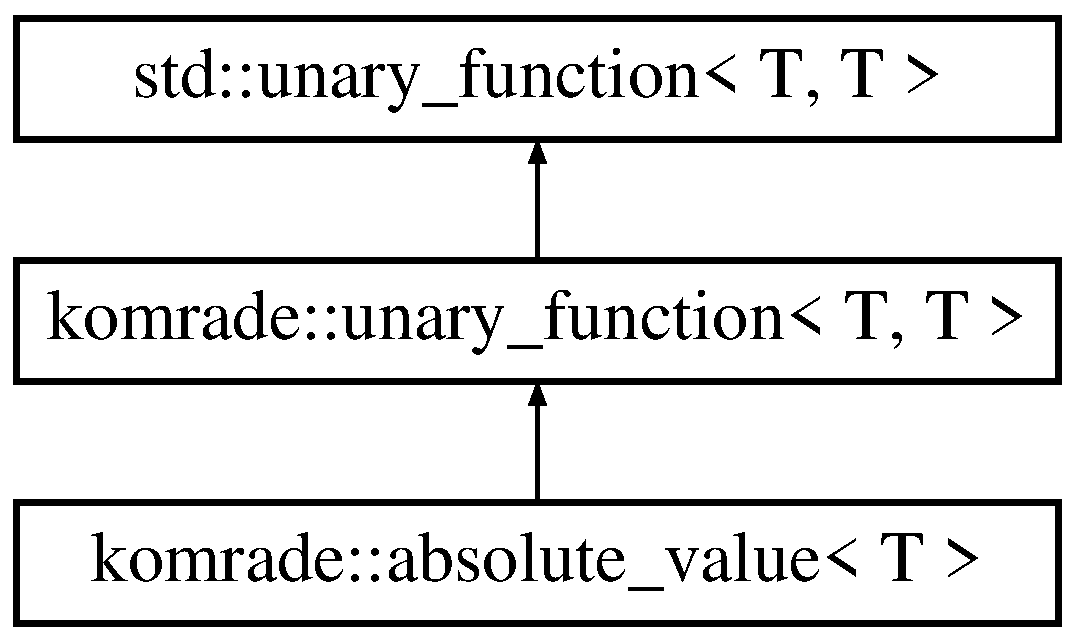
\includegraphics[height=3cm]{structkomrade_1_1absolute__value}
\end{center}
\end{figure}
\subsection*{Public Member Functions}
\begin{CompactItemize}
\item 
\_\-\_\-host\_\-\_\- \_\-\_\-device\_\-\_\- T {\bf operator()} (const T \&x) const 
\end{CompactItemize}


\subsection{Detailed Description}
\subsubsection*{template$<$typename T$>$ struct komrade::absolute\_\-value$<$ T $>$}

{\tt \doxyref{absolute\_\-value}{p.}{structkomrade_1_1absolute__value}} is a function object. Specifically, it is an Adaptable Unary Function. If {\tt f} is an object of class {\tt \doxyref{absolute\_\-value}{p.}{structkomrade_1_1absolute__value}}, and {\tt x} is an object of class {\tt T}, then {\tt f(x)} returns {\tt x $<$ 0 ? -x : x}.

\begin{Desc}
\item[Template Parameters:]
\begin{description}
\item[{\em T}]is a model of {\tt Assignable}, and {\tt T} is a model of {\tt LessThan Comparable}, and {\tt T(0)} must be defined.\end{description}
\end{Desc}
The following code snippet demonstrates how to use {\tt \doxyref{absolute\_\-value}{p.}{structkomrade_1_1absolute__value}} to find the magnitudes of a \doxyref{device\_\-vector}{p.}{classkomrade_1_1device__vector} of {\tt floats}.



\begin{Code}\begin{verbatim}  #include <komrade/device_vector.h>
  #include <komrade/functional.h>
  #include <komrade/range.h>
  #include <komrade/transform.h>
  ...
  const int N = 1000;
  komrade::device_vector<float> V1(N);
  komrade::device_vector<float> V2(N);

  komrade::range(V1.begin(), V1.end(), 1, -1);
  // V1 is now {-1, -2, -3, ..., -1000}

  komrade::transform(V1.begin(), V1.end(), V2.begin(),
                     komrade::absolute_value<float>());
  // V2 is now {1, 2, 3, ..., 1000}
\end{verbatim}
\end{Code}



\begin{Desc}
\item[See also:]\doxyref{unary\_\-function}{p.}{structkomrade_1_1unary__function} \end{Desc}


\subsection{Member Function Documentation}
\index{komrade::absolute\_\-value@{komrade::absolute\_\-value}!operator()@{operator()}}
\index{operator()@{operator()}!komrade::absolute_value@{komrade::absolute\_\-value}}
\subsubsection[operator()]{\setlength{\rightskip}{0pt plus 5cm}template$<$typename T$>$ \_\-\_\-host\_\-\_\- \_\-\_\-device\_\-\_\- T {\bf komrade::absolute\_\-value}$<$ T $>$::operator() (const T \& {\em x}) const\hspace{0.3cm}{\tt  [inline]}}\label{structkomrade_1_1absolute__value_9e7ce3d97b8accb50ef0c6e6df507aa7}


Function call operator. The return value is {\tt x $<$ 0 ? -x : x}. 

The documentation for this struct was generated from the following file:\begin{CompactItemize}
\item 
{\bf functional.h}\end{CompactItemize}

\section{komrade::bidirectional\_\-device\_\-iterator\_\-tag Struct Reference}
\label{structkomrade_1_1bidirectional__device__iterator__tag}\index{komrade::bidirectional\_\-device\_\-iterator\_\-tag@{komrade::bidirectional\_\-device\_\-iterator\_\-tag}}
{\tt \#include $<$iterator\_\-categories.h$>$}

Inheritance diagram for komrade::bidirectional\_\-device\_\-iterator\_\-tag::\begin{figure}[H]
\begin{center}
\leavevmode
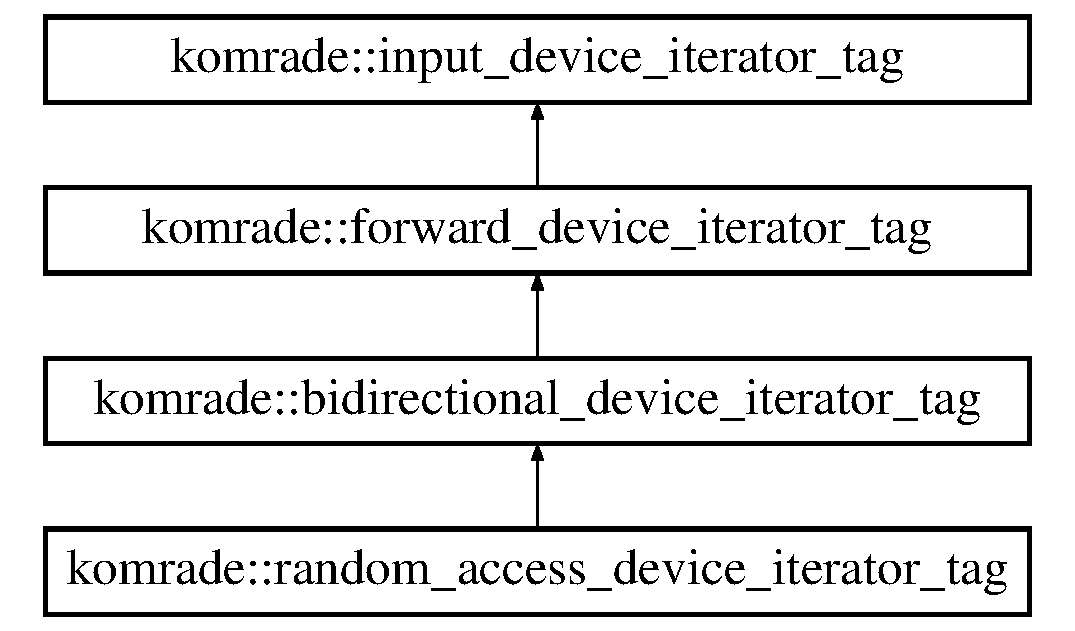
\includegraphics[height=4cm]{structkomrade_1_1bidirectional__device__iterator__tag}
\end{center}
\end{figure}


\subsection{Detailed Description}
{\tt \doxyref{bidirectional\_\-device\_\-iterator\_\-tag}{p.}{structkomrade_1_1bidirectional__device__iterator__tag}} is an empty class: it has no member functions, member variables, or nested types. It is used solely as a \char`\"{}tag\char`\"{}: a representation of the Bidirectional Device Iterator concept within the C++ type system.

\begin{Desc}
\item[See also:]{\tt http://www.sgi.com/tech/sgi/bidirectional\_\-iterator\_\-tag.html,} iterator\_\-traits, \doxyref{input\_\-device\_\-iterator\_\-tag}{p.}{structkomrade_1_1input__device__iterator__tag}, \doxyref{output\_\-device\_\-iterator\_\-tag}{p.}{structkomrade_1_1output__device__iterator__tag}, \doxyref{forward\_\-device\_\-iterator\_\-tag}{p.}{structkomrade_1_1forward__device__iterator__tag}, \doxyref{random\_\-access\_\-device\_\-iterator\_\-tag}{p.}{structkomrade_1_1random__access__device__iterator__tag}, \doxyref{input\_\-host\_\-iterator\_\-tag}{p.}{group__iterator__tag__classes_g0927e3a6aecf64b535bd28052c7516d5}, \doxyref{output\_\-host\_\-iterator\_\-tag}{p.}{group__iterator__tag__classes_gba20a59557406e3ab657831abf6d65a0}, \doxyref{forward\_\-host\_\-iterator\_\-tag}{p.}{group__iterator__tag__classes_gc0af280b47824bd61134805db6ffe828}, \doxyref{bidirectional\_\-host\_\-iterator\_\-tag}{p.}{group__iterator__tag__classes_gbdabd9cb52934a67a931cfd93d6079f0}, \doxyref{random\_\-access\_\-host\_\-iterator\_\-tag}{p.}{group__iterator__tag__classes_gfde808d31f9339adeda3dcf88077da8d} \end{Desc}


The documentation for this struct was generated from the following file:\begin{CompactItemize}
\item 
{\bf iterator\_\-categories.h}\end{CompactItemize}

\section{komrade::binary\_\-function$<$ Argument1, Argument2, Result $>$ Struct Template Reference}
\label{structkomrade_1_1binary__function}\index{komrade::binary\_\-function@{komrade::binary\_\-function}}
{\tt \#include $<$functional.h$>$}



\subsection{Detailed Description}
\subsubsection*{template$<$typename Argument1, typename Argument2, typename Result$>$ struct komrade::binary\_\-function$<$ Argument1, Argument2, Result $>$}

{\tt \doxyref{binary\_\-function}{p.}{structkomrade_1_1binary__function}} is an empty base class: it contains no member functions or member variables, but only type information. The only reason it exists is to make it more convenient to define types that are models of the concept Adaptable Binary Function. Specifically, any model of Adaptable Binary Function must define nested {\tt typedefs}. Those {\tt typedefs} are provided by the base class {\tt \doxyref{binary\_\-function}{p.}{structkomrade_1_1binary__function}}.

The following code snippet demonstrates how to construct an Adaptable Binary Function using {\tt \doxyref{binary\_\-function}{p.}{structkomrade_1_1binary__function}}.



\begin{Code}\begin{verbatim}  struct exponentiate : public komrade::binary_function<float,float,float>
  {
    __host__ __device__
    double operator()(float x, float y) { return powf(x,y); }
  };
\end{verbatim}
\end{Code}



\begin{Desc}
\item[Note:]\doxyref{binary\_\-function}{p.}{structkomrade_1_1binary__function} is currently redundant with the C++ STL type {\tt std::binary\_\-function}. We reserve it here for potential additional functionality at a later date.\end{Desc}
\begin{Desc}
\item[See also:]{\tt http://www.sgi.com/tech/stl/unary\_\-function.html} 

\doxyref{unary\_\-function}{p.}{structkomrade_1_1unary__function} \end{Desc}


The documentation for this struct was generated from the following file:\begin{CompactItemize}
\item 
{\bf functional.h}\end{CompactItemize}

\section{komrade::binary\_\-negate$<$ Predicate $>$ Struct Template Reference}
\label{structkomrade_1_1binary__negate}\index{komrade::binary\_\-negate@{komrade::binary\_\-negate}}
{\tt \#include $<$functional.h$>$}

\subsection*{Public Member Functions}
\begin{CompactItemize}
\item 
\_\-\_\-host\_\-\_\- \_\-\_\-device\_\-\_\- \textbf{binary\_\-negate} (Predicate p)\label{structkomrade_1_1binary__negate_1b2fd9d196377e76199f1de1f9ea8707}

\item 
{\footnotesize template$<$typename T$>$ }\\\_\-\_\-host\_\-\_\- \_\-\_\-device\_\-\_\- bool {\bf operator()} (const T x, const T y)
\end{CompactItemize}
\subsection*{Public Attributes}
\begin{CompactItemize}
\item 
Predicate \textbf{pred}\label{structkomrade_1_1binary__negate_7cbf855f00dd3a29f89ea4ff19c48182}

\end{CompactItemize}


\subsection{Detailed Description}
\subsubsection*{template$<$typename Predicate$>$ struct komrade::binary\_\-negate$<$ Predicate $>$}

{\tt \doxyref{binary\_\-negate}{p.}{structkomrade_1_1binary__negate}} is a function object adaptor: it is an Adaptable Binary Predicate that represents the logical negation of some other Adaptable Binary Predicate. That is: if {\tt f} is an object of class {\tt binary\_\-negate$<$AdaptablePredicate$>$}, then there exists an object {\tt pred} of class {\tt AdaptableBinaryPredicate} such that {\tt f(x,y)} always returns the same value as {\tt !pred(x,y)}. There is rarely any reason to construct a {\tt \doxyref{binary\_\-negate}{p.}{structkomrade_1_1binary__negate}} directly; it is almost always easier to use the helper function not2.

\begin{Desc}
\item[See also:]{\tt http://www.sgi.com/tech/stl/binary\_\-negate.html} \end{Desc}


\subsection{Member Function Documentation}
\index{komrade::binary\_\-negate@{komrade::binary\_\-negate}!operator()@{operator()}}
\index{operator()@{operator()}!komrade::binary_negate@{komrade::binary\_\-negate}}
\subsubsection[operator()]{\setlength{\rightskip}{0pt plus 5cm}template$<$typename Predicate$>$ template$<$typename T$>$ \_\-\_\-host\_\-\_\- \_\-\_\-device\_\-\_\- bool {\bf komrade::binary\_\-negate}$<$ Predicate $>$::operator() (const T {\em x}, \/  const T {\em y})\hspace{0.3cm}{\tt  [inline]}}\label{structkomrade_1_1binary__negate_c0e74423999d6af1e69e7608a77a2bfb}


Function call operator. The return value is {\tt !pred(x,y)}. 

The documentation for this struct was generated from the following file:\begin{CompactItemize}
\item 
{\bf functional.h}\end{CompactItemize}

\section{komrade::device\_\-allocator$<$ T $>$ Class Template Reference}
\label{classkomrade_1_1device__allocator}\index{komrade::device\_\-allocator@{komrade::device\_\-allocator}}
{\tt \#include $<$device\_\-allocator.h$>$}

Inheritance diagram for komrade::device\_\-allocator$<$ T $>$::\begin{figure}[H]
\begin{center}
\leavevmode
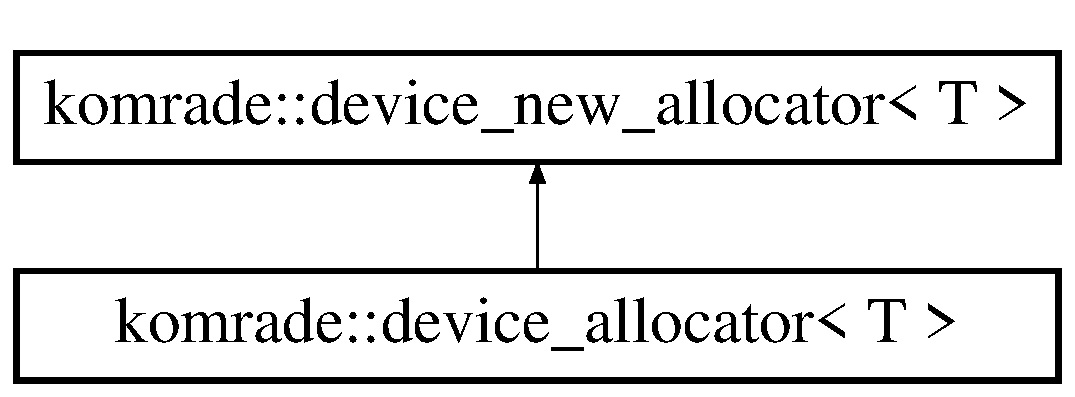
\includegraphics[height=2cm]{classkomrade_1_1device__allocator}
\end{center}
\end{figure}
\subsection*{Public Member Functions}
\begin{CompactItemize}
\item 
\_\-\_\-host\_\-\_\- \_\-\_\-device\_\-\_\- \textbf{device\_\-allocator} ({\bf device\_\-allocator} const \&)\label{classkomrade_1_1device__allocator_42dd5e07065e2469c0347dd808b05e4f}

\item 
{\footnotesize template$<$typename U$>$ }\\\_\-\_\-host\_\-\_\- \_\-\_\-device\_\-\_\- \textbf{device\_\-allocator} ({\bf device\_\-allocator}$<$ U $>$ const \&)\label{classkomrade_1_1device__allocator_b34139b9002b02b76c73baf52a8838fe}

\end{CompactItemize}
\subsection*{Classes}
\begin{CompactItemize}
\item 
struct \textbf{rebind}
\end{CompactItemize}


\subsection{Detailed Description}
\subsubsection*{template$<$typename T$>$ class komrade::device\_\-allocator$<$ T $>$}

{\tt \doxyref{device\_\-allocator}{p.}{classkomrade_1_1device__allocator}} is a device memory allocator. This implementation inherits from {\tt \doxyref{device\_\-new\_\-allocator}{p.}{classkomrade_1_1device__new__allocator}}.

\begin{Desc}
\item[See also:]\doxyref{device\_\-ptr}{p.}{structkomrade_1_1device__ptr} 

\doxyref{device\_\-new\_\-allocator}{p.}{classkomrade_1_1device__new__allocator} 

{\tt http://www.sgi.com/tech/stl/Allocators.html} \end{Desc}


The documentation for this class was generated from the following file:\begin{CompactItemize}
\item 
{\bf device\_\-allocator.h}\end{CompactItemize}

\section{komrade::device\_\-allocator$<$ void $>$ Class Template Reference}
\label{classkomrade_1_1device__allocator_3_01void_01_4}\index{komrade::device\_\-allocator$<$ void $>$@{komrade::device\_\-allocator$<$ void $>$}}
{\tt \#include $<$device\_\-allocator.h$>$}

\subsection*{Public Types}
\begin{CompactItemize}
\item 
typedef void \textbf{value\_\-type}\label{classkomrade_1_1device__allocator_3_01void_01_4_09604740b0a57974213bd9e2d3f2b8e0}

\item 
typedef {\bf device\_\-ptr}$<$ void $>$ \textbf{pointer}\label{classkomrade_1_1device__allocator_3_01void_01_4_837f7a2d74aea25c1d536f3ccafdf155}

\item 
typedef {\bf device\_\-ptr}$<$ const void $>$ \textbf{const\_\-pointer}\label{classkomrade_1_1device__allocator_3_01void_01_4_4c0c71a3e322ed98e92daed1235aa6f9}

\item 
typedef std::size\_\-t \textbf{size\_\-type}\label{classkomrade_1_1device__allocator_3_01void_01_4_29226c129b30950ad255b3abb8b34a04}

\item 
typedef pointer::difference\_\-type \textbf{difference\_\-type}\label{classkomrade_1_1device__allocator_3_01void_01_4_bcba41d997b0288c24a414ffebbda52a}

\end{CompactItemize}
\subsection*{Classes}
\begin{CompactItemize}
\item 
struct \textbf{rebind}
\end{CompactItemize}


\subsection{Detailed Description}
\subsubsection*{template$<$$>$ class komrade::device\_\-allocator$<$ void $>$}

{\tt \doxyref{device\_\-allocator$<$void$>$}{p.}{classkomrade_1_1device__allocator_3_01void_01_4}} is a device memory allocator. This class is a specialization for {\tt void}.

\begin{Desc}
\item[See also:]\doxyref{device\_\-ptr}{p.}{structkomrade_1_1device__ptr} 

{\tt http://www.sgi.com/tech/stl/Allocators.html} \end{Desc}


The documentation for this class was generated from the following file:\begin{CompactItemize}
\item 
{\bf device\_\-allocator.h}\end{CompactItemize}

\section{komrade::device\_\-new\_\-allocator$<$ T $>$ Class Template Reference}
\label{classkomrade_1_1device__new__allocator}\index{komrade::device\_\-new\_\-allocator@{komrade::device\_\-new\_\-allocator}}
{\tt \#include $<$device\_\-new\_\-allocator.h$>$}

Inheritance diagram for komrade::device\_\-new\_\-allocator$<$ T $>$::\begin{figure}[H]
\begin{center}
\leavevmode
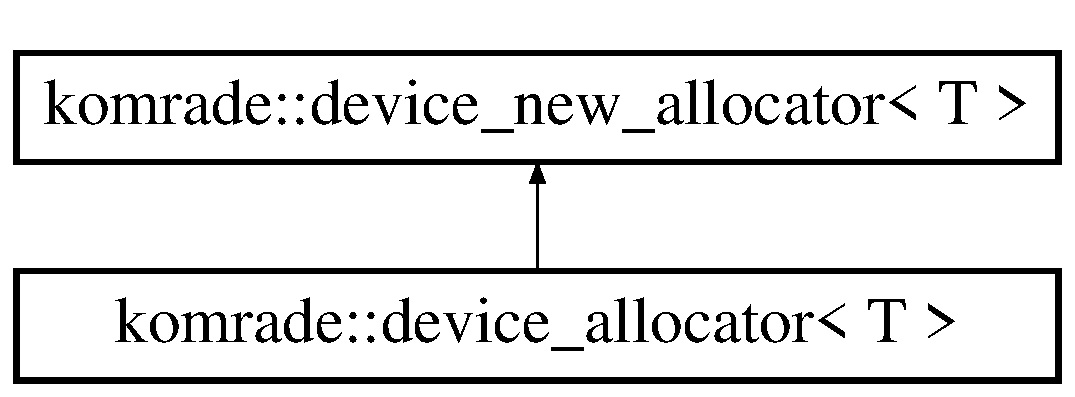
\includegraphics[height=2cm]{classkomrade_1_1device__new__allocator}
\end{center}
\end{figure}
\subsection*{Public Types}
\begin{CompactItemize}
\item 
typedef T \textbf{value\_\-type}\label{classkomrade_1_1device__new__allocator_1c38a2a83adab4ff7dde1de262f50b6f}

\item 
typedef {\bf device\_\-ptr}$<$ T $>$ \textbf{pointer}\label{classkomrade_1_1device__new__allocator_c60a6ca6d967fcf7437b4d6573fbb475}

\item 
typedef {\bf device\_\-ptr}$<$ const T $>$ \textbf{const\_\-pointer}\label{classkomrade_1_1device__new__allocator_b79ec03977e28bd4236b4e8c4589c284}

\item 
typedef {\bf device\_\-reference}$<$ T $>$ \textbf{reference}\label{classkomrade_1_1device__new__allocator_6077ee1ec11f65397f3a6e1c2b5dfd4e}

\item 
typedef {\bf device\_\-reference}$<$ const T $>$ \textbf{const\_\-reference}\label{classkomrade_1_1device__new__allocator_c2d09a04aeb87fdd93c2c428ce12eb56}

\item 
typedef std::size\_\-t \textbf{size\_\-type}\label{classkomrade_1_1device__new__allocator_4a624df53dcb813d43345d56f0827587}

\item 
typedef pointer::difference\_\-type \textbf{difference\_\-type}\label{classkomrade_1_1device__new__allocator_d44b11cb55aa29b715e18833d4e13eb7}

\end{CompactItemize}
\subsection*{Public Member Functions}
\begin{CompactItemize}
\item 
\_\-\_\-host\_\-\_\- \_\-\_\-device\_\-\_\- \textbf{device\_\-new\_\-allocator} ({\bf device\_\-new\_\-allocator} const \&)\label{classkomrade_1_1device__new__allocator_89aa3da79077ba3e65b05120f9e3f7c9}

\item 
{\footnotesize template$<$typename U$>$ }\\\_\-\_\-host\_\-\_\- \_\-\_\-device\_\-\_\- \textbf{device\_\-new\_\-allocator} ({\bf device\_\-new\_\-allocator}$<$ U $>$ const \&)\label{classkomrade_1_1device__new__allocator_158fdd4c1513cf171b6a6b39dc46f492}

\item 
\_\-\_\-host\_\-\_\- \_\-\_\-device\_\-\_\- {\bf pointer} \textbf{address} ({\bf reference} r)\label{classkomrade_1_1device__new__allocator_a0b8595c66fa6e67d5fafc268d78260d}

\item 
\_\-\_\-host\_\-\_\- \_\-\_\-device\_\-\_\- {\bf const\_\-pointer} \textbf{address} ({\bf const\_\-reference} r)\label{classkomrade_1_1device__new__allocator_bc8e4d1ebd3a1731bc5cef5eeb5bad35}

\item 
\_\-\_\-host\_\-\_\- {\bf pointer} \textbf{allocate} (size\_\-type cnt, {\bf const\_\-pointer}={\bf const\_\-pointer}(static\_\-cast$<$ T $\ast$ $>$(0)))\label{classkomrade_1_1device__new__allocator_67cef3a9252b6a2d45d3e7c27218374e}

\item 
\_\-\_\-host\_\-\_\- void \textbf{deallocate} ({\bf pointer} p, size\_\-type cnt)\label{classkomrade_1_1device__new__allocator_93dc5b8b6d6f99da53ce0ead01715435}

\item 
\_\-\_\-host\_\-\_\- \_\-\_\-device\_\-\_\- size\_\-type \textbf{max\_\-size} () const \label{classkomrade_1_1device__new__allocator_5a1366a7015cce4d821e38685ddbfab0}

\item 
\_\-\_\-host\_\-\_\- \_\-\_\-device\_\-\_\- bool \textbf{operator==} ({\bf device\_\-new\_\-allocator} const \&)\label{classkomrade_1_1device__new__allocator_4d2c5d27fcfe8071d94cde3d962f3d6a}

\item 
\_\-\_\-host\_\-\_\- \_\-\_\-device\_\-\_\- bool \textbf{operator!=} ({\bf device\_\-new\_\-allocator} const \&a)\label{classkomrade_1_1device__new__allocator_d743904da57d65c236a68484e0fd7f19}

\end{CompactItemize}
\subsection*{Classes}
\begin{CompactItemize}
\item 
struct \textbf{rebind}
\end{CompactItemize}


\subsection{Detailed Description}
\subsubsection*{template$<$typename T$>$ class komrade::device\_\-new\_\-allocator$<$ T $>$}

{\tt \doxyref{device\_\-new\_\-allocator}{p.}{classkomrade_1_1device__new__allocator}} is a device memory allocator that employs the {\tt device\_\-new} function for allocation.

\begin{Desc}
\item[See also:]\doxyref{device\_\-new}{p.}{group__allocation__functions_g6ba2e5e53b2acf5cdfe8a3818d7ffe42} 

\doxyref{device\_\-ptr}{p.}{structkomrade_1_1device__ptr} 

{\tt http://www.sgi.com/tech/stl/Allocators.html} \end{Desc}


The documentation for this class was generated from the following file:\begin{CompactItemize}
\item 
{\bf device\_\-new\_\-allocator.h}\end{CompactItemize}

\section{komrade::device\_\-ptr$<$ T $>$ Struct Template Reference}
\label{structkomrade_1_1device__ptr}\index{komrade::device\_\-ptr@{komrade::device\_\-ptr}}
{\tt \#include $<$device\_\-ptr.h$>$}

\subsection*{Public Types}
\begin{CompactItemize}
\item 
typedef {\bf komrade::random\_\-access\_\-device\_\-iterator\_\-tag} \textbf{iterator\_\-category}\label{structkomrade_1_1device__ptr_bb1bf09af6be567bc8cb1b10e616cebb}

\item 
typedef T \textbf{value\_\-type}\label{structkomrade_1_1device__ptr_3c7ffd10b83015c49a1c1f2e48561451}

\item 
typedef ptrdiff\_\-t \textbf{difference\_\-type}\label{structkomrade_1_1device__ptr_aef14e2bbf9dac66f7895fa7556103f5}

\item 
typedef {\bf device\_\-ptr} \textbf{pointer}\label{structkomrade_1_1device__ptr_4cb89bf25f3f95246e9c615c0f33f60c}

\item 
typedef {\bf device\_\-reference}$<$ T $>$ \textbf{reference}\label{structkomrade_1_1device__ptr_77d9fbf1d7522909558fb587e197e535}

\end{CompactItemize}
\subsection*{Public Member Functions}
\begin{CompactItemize}
\item 
\_\-\_\-host\_\-\_\- \_\-\_\-device\_\-\_\- {\bf device\_\-ptr} (void)
\item 
{\footnotesize template$<$class Y$>$ }\\\_\-\_\-host\_\-\_\- \_\-\_\-device\_\-\_\- {\bf device\_\-ptr} (Y $\ast$ptr)
\item 
\_\-\_\-host\_\-\_\- \_\-\_\-device\_\-\_\- {\bf device\_\-ptr} (const {\bf device\_\-ptr}$<$ typename detail::remove\_\-const$<$ value\_\-type $>$::type $>$ \&ptr)
\item 
{\footnotesize template$<$typename U$>$ }\\\_\-\_\-host\_\-\_\- \_\-\_\-device\_\-\_\- {\bf operator device\_\-ptr$<$ U $>$} (void) const 
\item 
\_\-\_\-host\_\-\_\- \_\-\_\-device\_\-\_\- {\bf device\_\-ptr} {\bf operator+} (const difference\_\-type \&rhs) const 
\item 
\_\-\_\-host\_\-\_\- \_\-\_\-device\_\-\_\- {\bf device\_\-ptr} {\bf operator-} (const difference\_\-type \&rhs) const 
\item 
\_\-\_\-host\_\-\_\- \_\-\_\-device\_\-\_\- {\bf device\_\-ptr} \& {\bf operator++} (void)
\item 
\_\-\_\-host\_\-\_\- \_\-\_\-device\_\-\_\- {\bf device\_\-ptr} {\bf operator++} (int)
\item 
\_\-\_\-host\_\-\_\- \_\-\_\-device\_\-\_\- {\bf device\_\-ptr} \& {\bf operator--} (void)
\item 
\_\-\_\-host\_\-\_\- \_\-\_\-device\_\-\_\- {\bf device\_\-ptr} {\bf operator--} (int)
\item 
\_\-\_\-host\_\-\_\- \_\-\_\-device\_\-\_\- {\bf device\_\-ptr} \& {\bf operator+=} (difference\_\-type rhs)
\item 
\_\-\_\-host\_\-\_\- \_\-\_\-device\_\-\_\- {\bf device\_\-ptr} \& {\bf operator-=} (difference\_\-type rhs)
\item 
\_\-\_\-host\_\-\_\- \_\-\_\-device\_\-\_\- difference\_\-type {\bf operator-} (const {\bf device\_\-ptr} \&rhs) const 
\item 
\_\-\_\-host\_\-\_\- \_\-\_\-device\_\-\_\- {\bf reference} {\bf operator[$\,$]} (const difference\_\-type \&i) const 
\item 
\_\-\_\-host\_\-\_\- \_\-\_\-device\_\-\_\- {\bf reference} {\bf operator$\ast$} (void) const 
\item 
\_\-\_\-host\_\-\_\- \_\-\_\-device\_\-\_\- value\_\-type $\ast$ {\bf get} (void) const 
\end{CompactItemize}
\subsection*{Friends}
\begin{CompactItemize}
\item 
struct \textbf{komrade::detail::device\_\-dereferenceable\_\-iterator\_\-traits$<$ komrade::device\_\-ptr$<$ T $>$ $>$}\label{structkomrade_1_1device__ptr_7ab0392dca3240ab3902abcee84faf71}

\item 
struct \textbf{komrade::detail::make\_\-device\_\-dereferenceable$<$ komrade::device\_\-ptr$<$ T $>$ $>$}\label{structkomrade_1_1device__ptr_a242c5c2d83b1c2b2861ee94296ac9c8}

\end{CompactItemize}


\subsection{Detailed Description}
\subsubsection*{template$<$typename T$>$ struct komrade::device\_\-ptr$<$ T $>$}

{\tt \doxyref{device\_\-ptr}{p.}{structkomrade_1_1device__ptr}} stores a pointer to an object allocated in device memory. This type provides type safety when dispatching standard algorithms on ranges resident in device memory.

{\tt \doxyref{device\_\-ptr}{p.}{structkomrade_1_1device__ptr}} can be created with the functions device\_\-malloc, device\_\-new, or device\_\-pointer\_\-cast, or by explicitly calling its constructor with a raw pointer.

The raw pointer encapsulated by a {\tt \doxyref{device\_\-ptr}{p.}{structkomrade_1_1device__ptr}} may be obtained by either its {\tt get} method or the device\_\-pointer\_\-cast free function.

\begin{Desc}
\item[Note:]{\tt \doxyref{device\_\-ptr}{p.}{structkomrade_1_1device__ptr}} is not a smart pointer; it is the programmer's responsibility to deallocate memory pointed to by {\tt \doxyref{device\_\-ptr}{p.}{structkomrade_1_1device__ptr}}.\end{Desc}
\begin{Desc}
\item[See also:]\doxyref{device\_\-malloc}{p.}{group__allocation__functions_g2344cbff21562ec9a109c7cd44999c90} 

\doxyref{device\_\-new}{p.}{group__allocation__functions_g6ba2e5e53b2acf5cdfe8a3818d7ffe42} 

\doxyref{device\_\-pointer\_\-cast}{p.}{group__memory__management__functions_g8fbaf7ffddae21678ed7afc19ff889c6} 

\doxyref{raw\_\-pointer\_\-cast}{p.}{group__memory__management__functions_g7d1643dacb28a3e6ca24f5972ed32dc9} \end{Desc}


\subsection{Constructor \& Destructor Documentation}
\index{komrade::device\_\-ptr@{komrade::device\_\-ptr}!device\_\-ptr@{device\_\-ptr}}
\index{device\_\-ptr@{device\_\-ptr}!komrade::device_ptr@{komrade::device\_\-ptr}}
\subsubsection[device\_\-ptr]{\setlength{\rightskip}{0pt plus 5cm}template$<$typename T$>$ \_\-\_\-host\_\-\_\- \_\-\_\-device\_\-\_\- {\bf komrade::device\_\-ptr}$<$ T $>$::{\bf device\_\-ptr} (void)\hspace{0.3cm}{\tt  [inline]}}\label{structkomrade_1_1device__ptr_7c07b668db696b71efdfed37fce6407e}


{\tt device\_\-ptr's} null constructor initializes its raw pointer to {\tt 0}. 

Referenced by komrade::device\_\-ptr$<$ T $>$::operator+(), and komrade::device\_\-ptr$<$ T $>$::operator-().\index{komrade::device\_\-ptr@{komrade::device\_\-ptr}!device\_\-ptr@{device\_\-ptr}}
\index{device\_\-ptr@{device\_\-ptr}!komrade::device_ptr@{komrade::device\_\-ptr}}
\subsubsection[device\_\-ptr]{\setlength{\rightskip}{0pt plus 5cm}template$<$typename T$>$ template$<$class Y$>$ \_\-\_\-host\_\-\_\- \_\-\_\-device\_\-\_\- {\bf komrade::device\_\-ptr}$<$ T $>$::{\bf device\_\-ptr} (Y $\ast$ {\em ptr})\hspace{0.3cm}{\tt  [inline, explicit]}}\label{structkomrade_1_1device__ptr_d93f0d18fde4d3a8c949d9b35522cd99}


{\tt device\_\-ptr's} copy constructor is templated to allow copying to a const T $\ast$ from a T $\ast$.

\begin{Desc}
\item[Parameters:]
\begin{description}
\item[{\em ptr}]A raw pointer to copy from, presumed to point to a location in device memory. \end{description}
\end{Desc}
\index{komrade::device\_\-ptr@{komrade::device\_\-ptr}!device\_\-ptr@{device\_\-ptr}}
\index{device\_\-ptr@{device\_\-ptr}!komrade::device_ptr@{komrade::device\_\-ptr}}
\subsubsection[device\_\-ptr]{\setlength{\rightskip}{0pt plus 5cm}template$<$typename T$>$ \_\-\_\-host\_\-\_\- \_\-\_\-device\_\-\_\- {\bf komrade::device\_\-ptr}$<$ T $>$::{\bf device\_\-ptr} (const {\bf device\_\-ptr}$<$ typename detail::remove\_\-const$<$ value\_\-type $>$::type $>$ \& {\em ptr})\hspace{0.3cm}{\tt  [inline]}}\label{structkomrade_1_1device__ptr_8cac342a978012968789bc25a0b10386}


{\tt device\_\-ptr's} copy constructor allows copying from another \doxyref{device\_\-ptr}{p.}{structkomrade_1_1device__ptr} with related type. \begin{Desc}
\item[Parameters:]
\begin{description}
\item[{\em ptr}]The {\tt \doxyref{device\_\-ptr}{p.}{structkomrade_1_1device__ptr}} to copy from. \end{description}
\end{Desc}


\subsection{Member Function Documentation}
\index{komrade::device\_\-ptr@{komrade::device\_\-ptr}!operator device\_\-ptr$<$ U $>$@{operator device\_\-ptr$<$ U $>$}}
\index{operator device\_\-ptr$<$ U $>$@{operator device\_\-ptr$<$ U $>$}!komrade::device_ptr@{komrade::device\_\-ptr}}
\subsubsection[operator device\_\-ptr$<$ U $>$]{\setlength{\rightskip}{0pt plus 5cm}template$<$typename T$>$ template$<$typename U$>$ \_\-\_\-host\_\-\_\- \_\-\_\-device\_\-\_\- {\bf komrade::device\_\-ptr}$<$ T $>$::operator {\bf device\_\-ptr}$<$ U $>$ (void) const\hspace{0.3cm}{\tt  [inline]}}\label{structkomrade_1_1device__ptr_8721b809d4fba8bf65f51c2146135351}


{\tt device\_\-ptr's} conversion operator allows conversion to {\tt device\_\-ptr$<$U$>$} with {\tt U} related to {\tt T}. For example, {\tt device\_\-ptr$<$int$>$} may be converted to {\tt device\_\-ptr$<$void$>$}.

\begin{Desc}
\item[Returns:]A copy of this {\tt \doxyref{device\_\-ptr}{p.}{structkomrade_1_1device__ptr}}, converted to {\tt device\_\-ptr$<$U$>$}. \end{Desc}
\index{komrade::device\_\-ptr@{komrade::device\_\-ptr}!operator+@{operator+}}
\index{operator+@{operator+}!komrade::device_ptr@{komrade::device\_\-ptr}}
\subsubsection[operator+]{\setlength{\rightskip}{0pt plus 5cm}template$<$typename T$>$ \_\-\_\-host\_\-\_\- \_\-\_\-device\_\-\_\- {\bf device\_\-ptr} {\bf komrade::device\_\-ptr}$<$ T $>$::operator+ (const difference\_\-type \& {\em rhs}) const\hspace{0.3cm}{\tt  [inline]}}\label{structkomrade_1_1device__ptr_f04ed4fefa306bafc4aa6bbe0f781b6e}


Returns a {\tt \doxyref{device\_\-ptr}{p.}{structkomrade_1_1device__ptr}} whose raw pointer is equal to this {\tt device\_\-ptr's} raw pointer \doxyref{plus}{p.}{structkomrade_1_1plus} the given sum.

\begin{Desc}
\item[Parameters:]
\begin{description}
\item[{\em rhs}]The sum to add to this {\tt device\_\-ptr's} raw pointer. \end{description}
\end{Desc}
\begin{Desc}
\item[Returns:]{\tt \doxyref{device\_\-ptr}{p.}{structkomrade_1_1device__ptr}(mPtr + rhs)}. \end{Desc}


References komrade::device\_\-ptr$<$ T $>$::device\_\-ptr().\index{komrade::device\_\-ptr@{komrade::device\_\-ptr}!operator-@{operator-}}
\index{operator-@{operator-}!komrade::device_ptr@{komrade::device\_\-ptr}}
\subsubsection[operator-]{\setlength{\rightskip}{0pt plus 5cm}template$<$typename T$>$ \_\-\_\-host\_\-\_\- \_\-\_\-device\_\-\_\- {\bf device\_\-ptr} {\bf komrade::device\_\-ptr}$<$ T $>$::operator- (const difference\_\-type \& {\em rhs}) const\hspace{0.3cm}{\tt  [inline]}}\label{structkomrade_1_1device__ptr_4a627df4c3313624ff247530461f5d48}


Returns a {\tt \doxyref{device\_\-ptr}{p.}{structkomrade_1_1device__ptr}} whose raw pointer is equal to this {\tt device\_\-ptr's} raw pointer \doxyref{minus}{p.}{structkomrade_1_1minus} the given difference.

\begin{Desc}
\item[Parameters:]
\begin{description}
\item[{\em rhs}]The difference to subtract to this {\tt device\_\-ptr's} raw pointer. \end{description}
\end{Desc}
\begin{Desc}
\item[Returns:]{\tt \doxyref{device\_\-ptr}{p.}{structkomrade_1_1device__ptr}(mPtr - rhs)}. \end{Desc}


References komrade::device\_\-ptr$<$ T $>$::device\_\-ptr().\index{komrade::device\_\-ptr@{komrade::device\_\-ptr}!operator++@{operator++}}
\index{operator++@{operator++}!komrade::device_ptr@{komrade::device\_\-ptr}}
\subsubsection[operator++]{\setlength{\rightskip}{0pt plus 5cm}template$<$typename T$>$ \_\-\_\-host\_\-\_\- \_\-\_\-device\_\-\_\- {\bf device\_\-ptr}\& {\bf komrade::device\_\-ptr}$<$ T $>$::operator++ (void)\hspace{0.3cm}{\tt  [inline]}}\label{structkomrade_1_1device__ptr_8aff1091af1dd73007c099398eb40ad8}


The pre-increment operator increments this {\tt device\_\-ptr's} raw pointer and then returns a reference to this {\tt \doxyref{device\_\-ptr}{p.}{structkomrade_1_1device__ptr}} \begin{Desc}
\item[Returns:]{\tt $\ast$this} \end{Desc}
\index{komrade::device\_\-ptr@{komrade::device\_\-ptr}!operator++@{operator++}}
\index{operator++@{operator++}!komrade::device_ptr@{komrade::device\_\-ptr}}
\subsubsection[operator++]{\setlength{\rightskip}{0pt plus 5cm}template$<$typename T$>$ \_\-\_\-host\_\-\_\- \_\-\_\-device\_\-\_\- {\bf device\_\-ptr} {\bf komrade::device\_\-ptr}$<$ T $>$::operator++ (int)\hspace{0.3cm}{\tt  [inline]}}\label{structkomrade_1_1device__ptr_07bf66f88d754498f40b36726dc47f3c}


The post-increment operator copies this {\tt \doxyref{device\_\-ptr}{p.}{structkomrade_1_1device__ptr}}, increments the copy, and then returns the copy. \begin{Desc}
\item[Returns:]A copy of this {\tt \doxyref{device\_\-ptr}{p.}{structkomrade_1_1device__ptr}} after being incremented. \end{Desc}


References komrade::copy().\index{komrade::device\_\-ptr@{komrade::device\_\-ptr}!operator--@{operator--}}
\index{operator--@{operator--}!komrade::device_ptr@{komrade::device\_\-ptr}}
\subsubsection[operator--]{\setlength{\rightskip}{0pt plus 5cm}template$<$typename T$>$ \_\-\_\-host\_\-\_\- \_\-\_\-device\_\-\_\- {\bf device\_\-ptr}\& {\bf komrade::device\_\-ptr}$<$ T $>$::operator-- (void)\hspace{0.3cm}{\tt  [inline]}}\label{structkomrade_1_1device__ptr_09431ef7a456b812236b58778fba50b0}


The pre-decrement operator decrements this {\tt device\_\-ptr's} raw pointer and then returns a reference to this {\tt \doxyref{device\_\-ptr}{p.}{structkomrade_1_1device__ptr}} \begin{Desc}
\item[Returns:]{\tt $\ast$this} \end{Desc}
\index{komrade::device\_\-ptr@{komrade::device\_\-ptr}!operator--@{operator--}}
\index{operator--@{operator--}!komrade::device_ptr@{komrade::device\_\-ptr}}
\subsubsection[operator--]{\setlength{\rightskip}{0pt plus 5cm}template$<$typename T$>$ \_\-\_\-host\_\-\_\- \_\-\_\-device\_\-\_\- {\bf device\_\-ptr} {\bf komrade::device\_\-ptr}$<$ T $>$::operator-- (int)\hspace{0.3cm}{\tt  [inline]}}\label{structkomrade_1_1device__ptr_cd716fbd99c4a0450aea4b6270922cc1}


The post-decrement operator copies this {\tt \doxyref{device\_\-ptr}{p.}{structkomrade_1_1device__ptr}}, decrements the copy, and then returns the copy. \begin{Desc}
\item[Returns:]A copy of this {\tt \doxyref{device\_\-ptr}{p.}{structkomrade_1_1device__ptr}} after being decremented. \end{Desc}


References komrade::copy().\index{komrade::device\_\-ptr@{komrade::device\_\-ptr}!operator+=@{operator+=}}
\index{operator+=@{operator+=}!komrade::device_ptr@{komrade::device\_\-ptr}}
\subsubsection[operator+=]{\setlength{\rightskip}{0pt plus 5cm}template$<$typename T$>$ \_\-\_\-host\_\-\_\- \_\-\_\-device\_\-\_\- {\bf device\_\-ptr}\& {\bf komrade::device\_\-ptr}$<$ T $>$::operator+= (difference\_\-type {\em rhs})\hspace{0.3cm}{\tt  [inline]}}\label{structkomrade_1_1device__ptr_ed7d610fbc9149d41ac43f087fa3bf64}


The addition assignment operator adds the given sum to this {\tt device\_\-ptr's} raw pointer and returns this {\tt \doxyref{device\_\-ptr}{p.}{structkomrade_1_1device__ptr}} by reference.

\begin{Desc}
\item[Parameters:]
\begin{description}
\item[{\em rhs}]The sum to add to this {\tt device\_\-ptr's} raw pointer. \end{description}
\end{Desc}
\begin{Desc}
\item[Returns:]{\tt $\ast$this} \end{Desc}
\index{komrade::device\_\-ptr@{komrade::device\_\-ptr}!operator-=@{operator-=}}
\index{operator-=@{operator-=}!komrade::device_ptr@{komrade::device\_\-ptr}}
\subsubsection[operator-=]{\setlength{\rightskip}{0pt plus 5cm}template$<$typename T$>$ \_\-\_\-host\_\-\_\- \_\-\_\-device\_\-\_\- {\bf device\_\-ptr}\& {\bf komrade::device\_\-ptr}$<$ T $>$::operator-= (difference\_\-type {\em rhs})\hspace{0.3cm}{\tt  [inline]}}\label{structkomrade_1_1device__ptr_e9d172eaed8cb95b5ba875feb01b0714}


The subtraction assignment operator subtracts the given difference from this {\tt device\_\-ptr's} raw pointer and returns this {\tt \doxyref{device\_\-ptr}{p.}{structkomrade_1_1device__ptr}} by reference.

\begin{Desc}
\item[Parameters:]
\begin{description}
\item[{\em rhs}]The difference to subtract from this {\tt device\_\-ptr's} raw pointer. \end{description}
\end{Desc}
\begin{Desc}
\item[Returns:]{\tt $\ast$this} \end{Desc}
\index{komrade::device\_\-ptr@{komrade::device\_\-ptr}!operator-@{operator-}}
\index{operator-@{operator-}!komrade::device_ptr@{komrade::device\_\-ptr}}
\subsubsection[operator-]{\setlength{\rightskip}{0pt plus 5cm}template$<$typename T$>$ \_\-\_\-host\_\-\_\- \_\-\_\-device\_\-\_\- difference\_\-type {\bf komrade::device\_\-ptr}$<$ T $>$::operator- (const {\bf device\_\-ptr}$<$ T $>$ \& {\em rhs}) const\hspace{0.3cm}{\tt  [inline]}}\label{structkomrade_1_1device__ptr_019534d131a828dee57dee08bd8221a5}


The difference operator returns the difference between this {\tt device\_\-ptr's} raw pointer and that of another.

\begin{Desc}
\item[Parameters:]
\begin{description}
\item[{\em rhs}]The {\tt \doxyref{device\_\-ptr}{p.}{structkomrade_1_1device__ptr}} to subtract from this {\tt \doxyref{device\_\-ptr}{p.}{structkomrade_1_1device__ptr}}. \end{description}
\end{Desc}
\begin{Desc}
\item[Returns:]The difference between this {\tt device\_\-ptr's} raw pointer and {\tt rhs's} raw pointer. \end{Desc}


References komrade::device\_\-ptr$<$ T $>$::mPtr.\index{komrade::device\_\-ptr@{komrade::device\_\-ptr}!operator[]@{operator[]}}
\index{operator[]@{operator[]}!komrade::device_ptr@{komrade::device\_\-ptr}}
\subsubsection[operator[]]{\setlength{\rightskip}{0pt plus 5cm}template$<$typename T$>$ \_\-\_\-host\_\-\_\- \_\-\_\-device\_\-\_\- {\bf reference} {\bf komrade::device\_\-ptr}$<$ T $>$::operator[$\,$] (const difference\_\-type \& {\em i}) const}\label{structkomrade_1_1device__ptr_96523226d9dd58d045618436837aa033}


The array subscript operator dereferences this {\tt \doxyref{device\_\-ptr}{p.}{structkomrade_1_1device__ptr}} by the given index. \begin{Desc}
\item[Parameters:]
\begin{description}
\item[{\em i}]The index to add to this {\tt device\_\-ptr's} raw pointer before deference. \end{description}
\end{Desc}
\begin{Desc}
\item[Returns:]A \doxyref{device\_\-reference}{p.}{structkomrade_1_1device__reference} referring to the object pointed to by (this {\tt \doxyref{device\_\-ptr}{p.}{structkomrade_1_1device__ptr}} \doxyref{plus}{p.}{structkomrade_1_1plus} {\tt i}). \end{Desc}
\index{komrade::device\_\-ptr@{komrade::device\_\-ptr}!operator$\ast$@{operator$\ast$}}
\index{operator$\ast$@{operator$\ast$}!komrade::device_ptr@{komrade::device\_\-ptr}}
\subsubsection[operator$\ast$]{\setlength{\rightskip}{0pt plus 5cm}template$<$typename T$>$ \_\-\_\-host\_\-\_\- \_\-\_\-device\_\-\_\- {\bf reference} {\bf komrade::device\_\-ptr}$<$ T $>$::operator$\ast$ (void) const}\label{structkomrade_1_1device__ptr_9f87c7ed2c0e190914b795291a5b8ef4}


This method dereferences this {\tt \doxyref{device\_\-ptr}{p.}{structkomrade_1_1device__ptr}}. \begin{Desc}
\item[Returns:]a \doxyref{device\_\-reference}{p.}{structkomrade_1_1device__reference} referring to the object pointed to by this {\tt \doxyref{device\_\-ptr}{p.}{structkomrade_1_1device__ptr}}. \end{Desc}
\index{komrade::device\_\-ptr@{komrade::device\_\-ptr}!get@{get}}
\index{get@{get}!komrade::device_ptr@{komrade::device\_\-ptr}}
\subsubsection[get]{\setlength{\rightskip}{0pt plus 5cm}template$<$typename T$>$ \_\-\_\-host\_\-\_\- \_\-\_\-device\_\-\_\- value\_\-type$\ast$ {\bf komrade::device\_\-ptr}$<$ T $>$::get (void) const\hspace{0.3cm}{\tt  [inline]}}\label{structkomrade_1_1device__ptr_8dcfd94ebfc66998aab5b15d172624b2}


This method returns this {\tt device\_\-ptr's} raw pointer. \begin{Desc}
\item[Returns:]This {\tt device\_\-ptr's} raw pointer. \end{Desc}


The documentation for this struct was generated from the following file:\begin{CompactItemize}
\item 
{\bf device\_\-ptr.h}\end{CompactItemize}

\section{komrade::device\_\-reference$<$ T $>$ Struct Template Reference}
\label{structkomrade_1_1device__reference}\index{komrade::device\_\-reference@{komrade::device\_\-reference}}
{\tt \#include $<$device\_\-reference.h$>$}

\subsection*{Public Types}
\begin{CompactItemize}
\item 
typedef {\bf device\_\-ptr}$<$ T $>$ \textbf{pointer}\label{structkomrade_1_1device__reference_753d18328ace929335e3f268e28b0f30}

\end{CompactItemize}
\subsection*{Public Member Functions}
\begin{CompactItemize}
\item 
{\bf device\_\-reference} (const {\bf device\_\-reference} \&ref)
\item 
{\bf device\_\-reference} (const {\bf pointer} \&ptr)
\item 
{\bf pointer} {\bf operator \&} (void) const 
\item 
{\bf device\_\-reference} \& {\bf operator=} (const T \&v)
\item 
{\bf device\_\-reference} \& {\bf operator=} (const {\bf device\_\-reference} \&ref)
\item 
{\bf device\_\-reference} \& {\bf operator++} (void)
\item 
T {\bf operator++} (int)
\item 
{\bf device\_\-reference} \& {\bf operator+=} (const T \&rhs)
\item 
{\bf device\_\-reference} \& {\bf operator--} (void)
\item 
T {\bf operator--} (int)
\item 
{\bf device\_\-reference} \& {\bf operator-=} (const T \&rhs)
\item 
{\bf device\_\-reference} \& {\bf operator$\ast$=} (const T \&rhs)
\item 
{\bf device\_\-reference} \& {\bf operator/=} (const T \&rhs)
\item 
{\bf device\_\-reference} \& {\bf operator\%=} (const T \&rhs)
\item 
{\bf device\_\-reference} \& {\bf operator$<$$<$=} (const T \&rhs)
\item 
{\bf device\_\-reference} \& {\bf operator$>$$>$=} (const T \&rhs)
\item 
{\bf device\_\-reference} \& {\bf operator \&=} (const T \&rhs)
\item 
{\bf device\_\-reference} \& {\bf operator$|$=} (const T \&rhs)
\item 
{\bf device\_\-reference} \& {\bf operator$^\wedge$=} (const T \&rhs)
\item 
{\bf operator T} (void) const 
\end{CompactItemize}


\subsection{Detailed Description}
\subsubsection*{template$<$typename T$>$ struct komrade::device\_\-reference$<$ T $>$}

{\tt \doxyref{device\_\-reference}{p.}{structkomrade_1_1device__reference}} acts as a reference to an object stored in device memory. {\tt \doxyref{device\_\-reference}{p.}{structkomrade_1_1device__reference}} is not intended to be used directly; rather, this type is the result of deferencing a {\tt \doxyref{device\_\-ptr}{p.}{structkomrade_1_1device__ptr}}. Similarly, taking the address of a {\tt \doxyref{device\_\-reference}{p.}{structkomrade_1_1device__reference}} yields a {\tt \doxyref{device\_\-ptr}{p.}{structkomrade_1_1device__ptr}}.

\begin{Desc}
\item[See also:]\doxyref{device\_\-ptr}{p.}{structkomrade_1_1device__ptr} \end{Desc}


\subsection{Constructor \& Destructor Documentation}
\index{komrade::device\_\-reference@{komrade::device\_\-reference}!device\_\-reference@{device\_\-reference}}
\index{device\_\-reference@{device\_\-reference}!komrade::device_reference@{komrade::device\_\-reference}}
\subsubsection[device\_\-reference]{\setlength{\rightskip}{0pt plus 5cm}template$<$typename T$>$ {\bf komrade::device\_\-reference}$<$ T $>$::{\bf device\_\-reference} (const {\bf device\_\-reference}$<$ T $>$ \& {\em ref})}\label{structkomrade_1_1device__reference_73b7480c6d3ddf8dd28c4576d92bd35f}


This copy constructor accepts a const reference to another {\tt \doxyref{device\_\-reference}{p.}{structkomrade_1_1device__reference}}. After this {\tt \doxyref{device\_\-reference}{p.}{structkomrade_1_1device__reference}} is constructed, it shall refer to the same object as {\tt ref}.

\begin{Desc}
\item[Parameters:]
\begin{description}
\item[{\em ref}]A {\tt \doxyref{device\_\-reference}{p.}{structkomrade_1_1device__reference}} to copy from.\end{description}
\end{Desc}
The following code snippet demonstrates the semantics of this copy constructor.



\begin{Code}\begin{verbatim}  #include <komrade/device_vector.h>
  #include <assert.h>
  ...
  komrade::device_vector<int> v(1,0);
  komrade::device_reference<int> ref = v[0];

  // ref equals the object at v[0]
  assert(ref1 == v[0]);

  // the address of ref equals the address of v[0]
  assert(&ref == &v[0]);

  // modifying v[0] modifies ref
  v[0] = 13;
  assert(ref == 13);
\end{verbatim}
\end{Code}

 \index{komrade::device\_\-reference@{komrade::device\_\-reference}!device\_\-reference@{device\_\-reference}}
\index{device\_\-reference@{device\_\-reference}!komrade::device_reference@{komrade::device\_\-reference}}
\subsubsection[device\_\-reference]{\setlength{\rightskip}{0pt plus 5cm}template$<$typename T$>$ {\bf komrade::device\_\-reference}$<$ T $>$::{\bf device\_\-reference} (const {\bf pointer} \& {\em ptr})\hspace{0.3cm}{\tt  [explicit]}}\label{structkomrade_1_1device__reference_2ffacbf48d87b2463d5a4799827b2296}


This copy constructor initializes this {\tt \doxyref{device\_\-reference}{p.}{structkomrade_1_1device__reference}} to refer to an object pointed to by the given {\tt \doxyref{device\_\-ptr}{p.}{structkomrade_1_1device__ptr}}. After this {\tt \doxyref{device\_\-reference}{p.}{structkomrade_1_1device__reference}} is constructed, it shall refer to the object pointed to by {\tt ptr}.

\begin{Desc}
\item[Parameters:]
\begin{description}
\item[{\em ptr}]A {\tt \doxyref{device\_\-ptr}{p.}{structkomrade_1_1device__ptr}} to copy from.\end{description}
\end{Desc}
The following code snippet demonstrates the semantic of this copy constructor.



\begin{Code}\begin{verbatim}  #include <komrade/device_vector.h>
  #include <assert.h>
  ...
  komrade::device_vector<int> v(1,0);
  komrade::device_ptr<int> ptr = &v[0];
  komrade::device_reference<int> ref(ptr);

  // ref equals the object pointed to by ptr
  assert(ref == *ptr);

  // the address of ref equals ptr
  assert(&ref == ptr);

  // modifying *ptr modifies ref
  *ptr = 13;
  assert(ref == 13);
\end{verbatim}
\end{Code}

 

\subsection{Member Function Documentation}
\index{komrade::device\_\-reference@{komrade::device\_\-reference}!operator \&@{operator \&}}
\index{operator \&@{operator \&}!komrade::device_reference@{komrade::device\_\-reference}}
\subsubsection[operator \&]{\setlength{\rightskip}{0pt plus 5cm}template$<$typename T$>$ {\bf pointer} {\bf komrade::device\_\-reference}$<$ T $>$::operator \& (void) const}\label{structkomrade_1_1device__reference_cf7c290d0f6e136fb3874eca896ebc6c}


Address-of operator returns a {\tt \doxyref{device\_\-ptr}{p.}{structkomrade_1_1device__ptr}} pointing to the object referenced by this {\tt \doxyref{device\_\-reference}{p.}{structkomrade_1_1device__reference}}. It does not return the address of this {\tt \doxyref{device\_\-reference}{p.}{structkomrade_1_1device__reference}}.

\begin{Desc}
\item[Returns:]A {\tt \doxyref{device\_\-ptr}{p.}{structkomrade_1_1device__ptr}} pointing to the object this {\tt \doxyref{device\_\-reference}{p.}{structkomrade_1_1device__reference}} references. \end{Desc}
\index{komrade::device\_\-reference@{komrade::device\_\-reference}!operator=@{operator=}}
\index{operator=@{operator=}!komrade::device_reference@{komrade::device\_\-reference}}
\subsubsection[operator=]{\setlength{\rightskip}{0pt plus 5cm}template$<$typename T$>$ {\bf device\_\-reference}\& {\bf komrade::device\_\-reference}$<$ T $>$::operator= (const T \& {\em v})}\label{structkomrade_1_1device__reference_baca91486692ade95366a10659143c4d}


Assignment operator copies the value of the given object to the object referenced by this {\tt \doxyref{device\_\-reference}{p.}{structkomrade_1_1device__reference}}.

\begin{Desc}
\item[Parameters:]
\begin{description}
\item[{\em v}]The value to copy from. \end{description}
\end{Desc}
\begin{Desc}
\item[Returns:]This {\tt \doxyref{device\_\-reference}{p.}{structkomrade_1_1device__reference}}. \end{Desc}
\index{komrade::device\_\-reference@{komrade::device\_\-reference}!operator=@{operator=}}
\index{operator=@{operator=}!komrade::device_reference@{komrade::device\_\-reference}}
\subsubsection[operator=]{\setlength{\rightskip}{0pt plus 5cm}template$<$typename T$>$ {\bf device\_\-reference}\& {\bf komrade::device\_\-reference}$<$ T $>$::operator= (const {\bf device\_\-reference}$<$ T $>$ \& {\em ref})}\label{structkomrade_1_1device__reference_d06369f1bf208eaa14a9349ca627c9fb}


Assignment operator copies the value of the object referenced by the given {\tt \doxyref{device\_\-reference}{p.}{structkomrade_1_1device__reference}} to the object referenced by this {\tt \doxyref{device\_\-reference}{p.}{structkomrade_1_1device__reference}}.

\begin{Desc}
\item[Parameters:]
\begin{description}
\item[{\em ref}]The {\tt \doxyref{device\_\-reference}{p.}{structkomrade_1_1device__reference}} to copy from. \end{description}
\end{Desc}
\begin{Desc}
\item[Returns:]This {\tt \doxyref{device\_\-reference}{p.}{structkomrade_1_1device__reference}}.\end{Desc}
\begin{Desc}
\item[{\bf Bug}]This needs to be templated on the type of the {\tt \doxyref{device\_\-reference}{p.}{structkomrade_1_1device__reference}} to copy from. \end{Desc}
\index{komrade::device\_\-reference@{komrade::device\_\-reference}!operator++@{operator++}}
\index{operator++@{operator++}!komrade::device_reference@{komrade::device\_\-reference}}
\subsubsection[operator++]{\setlength{\rightskip}{0pt plus 5cm}template$<$typename T$>$ {\bf device\_\-reference}\& {\bf komrade::device\_\-reference}$<$ T $>$::operator++ (void)}\label{structkomrade_1_1device__reference_147d08cc8f0f7cb4cd6f117bbf7a68c6}


Prefix increment operator increments the object referenced by this {\tt \doxyref{device\_\-reference}{p.}{structkomrade_1_1device__reference}}.

\begin{Desc}
\item[Returns:]{\tt $\ast$this}\end{Desc}
The following code snippet demonstrates the semantics of {\tt device\_\-reference's} prefix increment operator.



\begin{Code}\begin{verbatim}  #include <komrade/device_vector.h>
  #include <assert.h>
  ...
  komrade::device_vector<int> v(1,0);
  komrade::device_ptr<int> ptr = &v[0];
  komrade::device_reference<int> ref(ptr);

  // ref equals 0
  assert(ref == 0);

  // the object pointed to by ptr equals 1
  assert(*ptr == 1);

  // v[0] equals 1
  assert(v[0] == 1);

  // increment ref
  ++ref;

  // ref equals 1
  assert(ref == 1);

  // the object pointed to by ptr equals 1
  assert(*ptr == 1);

  // v[0] equals 1
  assert(v[0] == 1);
\end{verbatim}
\end{Code}



\begin{Desc}
\item[Note:]The increment executes as if it were executed on the host. This may change in a later version. \end{Desc}
\index{komrade::device\_\-reference@{komrade::device\_\-reference}!operator++@{operator++}}
\index{operator++@{operator++}!komrade::device_reference@{komrade::device\_\-reference}}
\subsubsection[operator++]{\setlength{\rightskip}{0pt plus 5cm}template$<$typename T$>$ T {\bf komrade::device\_\-reference}$<$ T $>$::operator++ (int)}\label{structkomrade_1_1device__reference_0ff1874a4e309269be43e28292b0232e}


Postfix increment operator copies the object referenced by this {\tt \doxyref{device\_\-reference}{p.}{structkomrade_1_1device__reference}}, increments the object referenced by this {\tt \doxyref{device\_\-reference}{p.}{structkomrade_1_1device__reference}}, and returns the copy.

\begin{Desc}
\item[Returns:]A copy of the object referenced by this {\tt \doxyref{device\_\-reference}{p.}{structkomrade_1_1device__reference}} before being incremented.\end{Desc}
The following code snippet demonstrates the semantics of {\tt device\_\-reference's} postfix increment operator.



\begin{Code}\begin{verbatim}  #include <komrade/device_vector.h>
  #include <assert.h>
  ...
  komrade::device_vector<int> v(1,0);
  komrade::device_ptr<int> ptr = &v[0];
  komrade::device_reference<int> ref(ptr);

  // ref equals 0
  assert(ref == 0);

  // the object pointed to by ptr equals 0
  assert(*ptr == 0);

  // v[0] equals 0
  assert(v[0] == 0);

  // increment ref
  int x = ref++;

  // x equals 0
  assert(x == 0)

  // ref equals 1
  assert(ref == 1);

  // the object pointed to by ptr equals 1
  assert(*ptr == 1);

  // v[0] equals 1
  assert(v[0] == 1);
\end{verbatim}
\end{Code}



\begin{Desc}
\item[Note:]The increment executes as if it were executed on the host. This may change in a later version. \end{Desc}
\index{komrade::device\_\-reference@{komrade::device\_\-reference}!operator+=@{operator+=}}
\index{operator+=@{operator+=}!komrade::device_reference@{komrade::device\_\-reference}}
\subsubsection[operator+=]{\setlength{\rightskip}{0pt plus 5cm}template$<$typename T$>$ {\bf device\_\-reference}\& {\bf komrade::device\_\-reference}$<$ T $>$::operator+= (const T \& {\em rhs})}\label{structkomrade_1_1device__reference_674b87c5778e6a2787915c73d26a382c}


Addition assignment operator add-assigns the object referenced by this {\tt \doxyref{device\_\-reference}{p.}{structkomrade_1_1device__reference}} and returns this {\tt \doxyref{device\_\-reference}{p.}{structkomrade_1_1device__reference}}.

\begin{Desc}
\item[Parameters:]
\begin{description}
\item[{\em rhs}]The right hand side of the add-assignment. \end{description}
\end{Desc}
\begin{Desc}
\item[Returns:]{\tt $\ast$this}.\end{Desc}
The following code snippet demonstrates the semantics of {\tt device\_\-reference's} addition assignment operator.



\begin{Code}\begin{verbatim}  #include <komrade/device_vector.h>
  #include <assert.h>
  ...
  komrade::device_vector<int> v(1,0);
  komrade::device_ptr<int> ptr = &v[0];
  komrade::device_reference<int> ref(ptr);

  // ref equals 0
  assert(ref == 0);

  // the object pointed to by ptr equals 0
  assert(*ptr == 0);

  // v[0] equals 0
  assert(v[0] == 0);

  // add-assign ref
  ref += 5;

  // ref equals 5
  assert(ref == 5);

  // the object pointed to by ptr equals 5
  assert(*ptr == 5);

  // v[0] equals 5
  assert(v[0] == 5);
\end{verbatim}
\end{Code}



\begin{Desc}
\item[Note:]The add-assignment executes as as if it were executed on the host. This may change in a later version. \end{Desc}
\index{komrade::device\_\-reference@{komrade::device\_\-reference}!operator--@{operator--}}
\index{operator--@{operator--}!komrade::device_reference@{komrade::device\_\-reference}}
\subsubsection[operator--]{\setlength{\rightskip}{0pt plus 5cm}template$<$typename T$>$ {\bf device\_\-reference}\& {\bf komrade::device\_\-reference}$<$ T $>$::operator-- (void)}\label{structkomrade_1_1device__reference_c4136765baf706e20a0651e54b55aa2c}


Prefix decrement operator decrements the object referenced by this {\tt \doxyref{device\_\-reference}{p.}{structkomrade_1_1device__reference}}.

\begin{Desc}
\item[Returns:]{\tt $\ast$this}\end{Desc}
The following code snippet demonstrates the semantics of {\tt device\_\-reference's} prefix decrement operator.



\begin{Code}\begin{verbatim}  #include <komrade/device_vector.h>
  #include <assert.h>
  ...
  komrade::device_vector<int> v(1,0);
  komrade::device_ptr<int> ptr = &v[0];
  komrade::device_reference<int> ref(ptr);

  // ref equals 0
  assert(ref == 0);

  // the object pointed to by ptr equals 0
  assert(*ptr == 0);

  // v[0] equals 0
  assert(v[0] == 0);

  // decrement ref
  --ref;

  // ref equals -1
  assert(ref == -1);

  // the object pointed to by ptr equals -1
  assert(*ptr == -1);

  // v[0] equals -1
  assert(v[0] == -1);
\end{verbatim}
\end{Code}



\begin{Desc}
\item[Note:]The decrement executes as if it were executed on the host. This may change in a later version. \end{Desc}
\index{komrade::device\_\-reference@{komrade::device\_\-reference}!operator--@{operator--}}
\index{operator--@{operator--}!komrade::device_reference@{komrade::device\_\-reference}}
\subsubsection[operator--]{\setlength{\rightskip}{0pt plus 5cm}template$<$typename T$>$ T {\bf komrade::device\_\-reference}$<$ T $>$::operator-- (int)}\label{structkomrade_1_1device__reference_59f56e121329965191ce7af2845398d5}


Postfix decrement operator copies the object referenced by this {\tt \doxyref{device\_\-reference}{p.}{structkomrade_1_1device__reference}}, decrements the object referenced by this {\tt \doxyref{device\_\-reference}{p.}{structkomrade_1_1device__reference}}, and returns the copy.

\begin{Desc}
\item[Returns:]A copy of the object referenced by this {\tt \doxyref{device\_\-reference}{p.}{structkomrade_1_1device__reference}} before being decremented.\end{Desc}
The following code snippet demonstrates the semantics of {\tt device\_\-reference's} postfix decrement operator.



\begin{Code}\begin{verbatim}  #include <komrade/device_vector.h>
  #include <assert.h>
  ...
  komrade::device_vector<int> v(1,0);
  komrade::device_ptr<int> ptr = &v[0];
  komrade::device_reference<int> ref(ptr);

  // ref equals 0
  assert(ref == 0);

  // the object pointed to by ptr equals 0
  assert(*ptr == 0);

  // v[0] equals 0
  assert(v[0] == 0);

  // decrement ref
  int x = ref--;

  // x equals 0
  assert(x == 0)

  // ref equals -1
  assert(ref == -1);

  // the object pointed to by ptr equals -1
  assert(*ptr == -1);

  // v[0] equals -1
  assert(v[0] == -1);
\end{verbatim}
\end{Code}



\begin{Desc}
\item[Note:]The decrement executes as if it were executed on the host. This may change in a later version. \end{Desc}
\index{komrade::device\_\-reference@{komrade::device\_\-reference}!operator-=@{operator-=}}
\index{operator-=@{operator-=}!komrade::device_reference@{komrade::device\_\-reference}}
\subsubsection[operator-=]{\setlength{\rightskip}{0pt plus 5cm}template$<$typename T$>$ {\bf device\_\-reference}\& {\bf komrade::device\_\-reference}$<$ T $>$::operator-= (const T \& {\em rhs})}\label{structkomrade_1_1device__reference_566df8124ae7b7981717e428b6f0edac}


Subtraction assignment operator subtract-assigns the object referenced by this {\tt \doxyref{device\_\-reference}{p.}{structkomrade_1_1device__reference}} and returns this {\tt \doxyref{device\_\-reference}{p.}{structkomrade_1_1device__reference}}.

\begin{Desc}
\item[Parameters:]
\begin{description}
\item[{\em rhs}]The right hand side of the subtraction-assignment. \end{description}
\end{Desc}
\begin{Desc}
\item[Returns:]{\tt $\ast$this}.\end{Desc}
The following code snippet demonstrates the semantics of {\tt device\_\-reference's} addition assignment operator.



\begin{Code}\begin{verbatim}  #include <komrade/device_vector.h>
  #include <assert.h>
  ...
  komrade::device_vector<int> v(1,0);
  komrade::device_ptr<int> ptr = &v[0];
  komrade::device_reference<int> ref(ptr);

  // ref equals 0
  assert(ref == 0);

  // the object pointed to by ptr equals 0
  assert(*ptr == 0);

  // v[0] equals 0
  assert(v[0] == 0);

  // subtract-assign ref
  ref -= 5;

  // ref equals -5
  assert(ref == -5);

  // the object pointed to by ptr equals -5
  assert(*ptr == -5);

  // v[0] equals -5
  assert(v[0] == -5);
\end{verbatim}
\end{Code}



\begin{Desc}
\item[Note:]The subtract-assignment executes as as if it were executed on the host. This may change in a later version. \end{Desc}
\index{komrade::device\_\-reference@{komrade::device\_\-reference}!operator$\ast$=@{operator$\ast$=}}
\index{operator$\ast$=@{operator$\ast$=}!komrade::device_reference@{komrade::device\_\-reference}}
\subsubsection[operator$\ast$=]{\setlength{\rightskip}{0pt plus 5cm}template$<$typename T$>$ {\bf device\_\-reference}\& {\bf komrade::device\_\-reference}$<$ T $>$::operator$\ast$= (const T \& {\em rhs})}\label{structkomrade_1_1device__reference_99a3cb30b3fadd3b8e1c5de5cb1f6e6e}


Multiplication assignment operator multiply-assigns the object referenced by this {\tt \doxyref{device\_\-reference}{p.}{structkomrade_1_1device__reference}} and returns this {\tt \doxyref{device\_\-reference}{p.}{structkomrade_1_1device__reference}}.

\begin{Desc}
\item[Parameters:]
\begin{description}
\item[{\em rhs}]The right hand side of the multiply-assignment. \end{description}
\end{Desc}
\begin{Desc}
\item[Returns:]{\tt $\ast$this}.\end{Desc}
The following code snippet demonstrates the semantics of {\tt device\_\-reference's} multiply assignment operator.



\begin{Code}\begin{verbatim}  #include <komrade/device_vector.h>
  #include <assert.h>
  ...
  komrade::device_vector<int> v(1,1);
  komrade::device_ptr<int> ptr = &v[0];
  komrade::device_reference<int> ref(ptr);

  // ref equals 1
  assert(ref == 1);

  // the object pointed to by ptr equals 1
  assert(*ptr == 1);

  // v[0] equals 1
  assert(v[0] == 1);

  // multiply-assign ref
  ref *= 5;

  // ref equals 5
  assert(ref == 5);

  // the object pointed to by ptr equals 5
  assert(*ptr == 5);

  // v[0] equals 5
  assert(v[0] == 5);
\end{verbatim}
\end{Code}



\begin{Desc}
\item[Note:]The multiply-assignment executes as as if it were executed on the host. This may change in a later version. \end{Desc}
\index{komrade::device\_\-reference@{komrade::device\_\-reference}!operator/=@{operator/=}}
\index{operator/=@{operator/=}!komrade::device_reference@{komrade::device\_\-reference}}
\subsubsection[operator/=]{\setlength{\rightskip}{0pt plus 5cm}template$<$typename T$>$ {\bf device\_\-reference}\& {\bf komrade::device\_\-reference}$<$ T $>$::operator/= (const T \& {\em rhs})}\label{structkomrade_1_1device__reference_60e9916869b637ba00a47f012336ac2e}


Division assignment operator divide-assigns the object referenced by this {\tt \doxyref{device\_\-reference}{p.}{structkomrade_1_1device__reference}} and returns this {\tt \doxyref{device\_\-reference}{p.}{structkomrade_1_1device__reference}}.

\begin{Desc}
\item[Parameters:]
\begin{description}
\item[{\em rhs}]The right hand side of the divide-assignment. \end{description}
\end{Desc}
\begin{Desc}
\item[Returns:]{\tt $\ast$this}.\end{Desc}
The following code snippet demonstrates the semantics of {\tt device\_\-reference's} divide assignment operator.



\begin{Code}\begin{verbatim}  #include <komrade/device_vector.h>
  #include <assert.h>
  ...
  komrade::device_vector<int> v(1,5);
  komrade::device_ptr<int> ptr = &v[0];
  komrade::device_reference<int> ref(ptr);

  // ref equals 5
  assert(ref == 5);

  // the object pointed to by ptr equals 5
  assert(*ptr == 5);

  // v[0] equals 5
  assert(v[0] == 5);

  // divide-assign ref
  ref /= 5;

  // ref equals 1
  assert(ref == 1);

  // the object pointed to by ptr equals 1
  assert(*ptr == 1);

  // v[0] equals 1
  assert(v[0] == 1);
\end{verbatim}
\end{Code}



\begin{Desc}
\item[Note:]The divide-assignment executes as as if it were executed on the host. This may change in a later version. \end{Desc}
\index{komrade::device\_\-reference@{komrade::device\_\-reference}!operator\%=@{operator\%=}}
\index{operator\%=@{operator\%=}!komrade::device_reference@{komrade::device\_\-reference}}
\subsubsection[operator\%=]{\setlength{\rightskip}{0pt plus 5cm}template$<$typename T$>$ {\bf device\_\-reference}\& {\bf komrade::device\_\-reference}$<$ T $>$::operator\%= (const T \& {\em rhs})}\label{structkomrade_1_1device__reference_0b0204c74cca61dc90d698eb0c62a881}


Modulation assignment operator modulus-assigns the object referenced by this {\tt \doxyref{device\_\-reference}{p.}{structkomrade_1_1device__reference}} and returns this {\tt \doxyref{device\_\-reference}{p.}{structkomrade_1_1device__reference}}.

\begin{Desc}
\item[Parameters:]
\begin{description}
\item[{\em rhs}]The right hand side of the divide-assignment. \end{description}
\end{Desc}
\begin{Desc}
\item[Returns:]{\tt $\ast$this}.\end{Desc}
The following code snippet demonstrates the semantics of {\tt device\_\-reference's} divide assignment operator.



\begin{Code}\begin{verbatim}  #include <komrade/device_vector.h>
  #include <assert.h>
  ...
  komrade::device_vector<int> v(1,5);
  komrade::device_ptr<int> ptr = &v[0];
  komrade::device_reference<int> ref(ptr);

  // ref equals 5
  assert(ref == 5);

  // the object pointed to by ptr equals 5
  assert(*ptr == 5);

  // v[0] equals 5
  assert(v[0] == 5);

  // modulus-assign ref
  ref %= 5;

  // ref equals 0
  assert(ref == 0);

  // the object pointed to by ptr equals 0
  assert(*ptr == 0);

  // v[0] equals 0
  assert(v[0] == 0);
\end{verbatim}
\end{Code}



\begin{Desc}
\item[Note:]The modulus-assignment executes as as if it were executed on the host. This may change in a later version. \end{Desc}
\index{komrade::device\_\-reference@{komrade::device\_\-reference}!operator$<$$<$=@{operator$<$$<$=}}
\index{operator$<$$<$=@{operator$<$$<$=}!komrade::device_reference@{komrade::device\_\-reference}}
\subsubsection[operator$<$$<$=]{\setlength{\rightskip}{0pt plus 5cm}template$<$typename T$>$ {\bf device\_\-reference}\& {\bf komrade::device\_\-reference}$<$ T $>$::operator$<$$<$= (const T \& {\em rhs})}\label{structkomrade_1_1device__reference_fe8da37546d0023df9dc97e604a480ee}


Bitwise left shift assignment operator left shift-assigns the object referenced by this {\tt \doxyref{device\_\-reference}{p.}{structkomrade_1_1device__reference}} and returns this {\tt \doxyref{device\_\-reference}{p.}{structkomrade_1_1device__reference}}.

\begin{Desc}
\item[Parameters:]
\begin{description}
\item[{\em rhs}]The right hand side of the left shift-assignment. \end{description}
\end{Desc}
\begin{Desc}
\item[Returns:]{\tt $\ast$this}.\end{Desc}
The following code snippet demonstrates the semantics of {\tt device\_\-reference's} left shift assignment operator.



\begin{Code}\begin{verbatim}  #include <komrade/device_vector.h>
  #include <assert.h>
  ...
  komrade::device_vector<int> v(1,1);
  komrade::device_ptr<int> ptr = &v[0];
  komrade::device_reference<int> ref(ptr);

  // ref equals 1
  assert(ref == 1);

  // the object pointed to by ptr equals 1
  assert(*ptr == 1);

  // v[0] equals 1
  assert(v[0] == 1);

  // left shift-assign ref
  ref <<= 1;

  // ref equals 2
  assert(ref == 2);

  // the object pointed to by ptr equals 2
  assert(*ptr == 2);

  // v[0] equals 2
  assert(v[0] == 2);
\end{verbatim}
\end{Code}



\begin{Desc}
\item[Note:]The left shift-assignment executes as as if it were executed on the host. This may change in a later version. \end{Desc}
\index{komrade::device\_\-reference@{komrade::device\_\-reference}!operator$>$$>$=@{operator$>$$>$=}}
\index{operator$>$$>$=@{operator$>$$>$=}!komrade::device_reference@{komrade::device\_\-reference}}
\subsubsection[operator$>$$>$=]{\setlength{\rightskip}{0pt plus 5cm}template$<$typename T$>$ {\bf device\_\-reference}\& {\bf komrade::device\_\-reference}$<$ T $>$::operator$>$$>$= (const T \& {\em rhs})}\label{structkomrade_1_1device__reference_67f5c159c698d2b2d232af8f093159df}


Bitwise right shift assignment operator right shift-assigns the object referenced by this {\tt \doxyref{device\_\-reference}{p.}{structkomrade_1_1device__reference}} and returns this {\tt \doxyref{device\_\-reference}{p.}{structkomrade_1_1device__reference}}.

\begin{Desc}
\item[Parameters:]
\begin{description}
\item[{\em rhs}]The right hand side of the right shift-assignment. \end{description}
\end{Desc}
\begin{Desc}
\item[Returns:]{\tt $\ast$this}.\end{Desc}
The following code snippet demonstrates the semantics of {\tt device\_\-reference's} right shift assignment operator.



\begin{Code}\begin{verbatim}  #include <komrade/device_vector.h>
  #include <assert.h>
  ...
  komrade::device_vector<int> v(1,2);
  komrade::device_ptr<int> ptr = &v[0];
  komrade::device_reference<int> ref(ptr);

  // ref equals 2
  assert(ref == 2);

  // the object pointed to by ptr equals 2
  assert(*ptr == 2);

  // v[0] equals 2
  assert(v[0] == 2);

  // right shift-assign ref
  ref >>= 1;

  // ref equals 1
  assert(ref == 1);

  // the object pointed to by ptr equals 1
  assert(*ptr == 1);

  // v[0] equals 1
  assert(v[0] == 1);
\end{verbatim}
\end{Code}



\begin{Desc}
\item[Note:]The right shift-assignment executes as as if it were executed on the host. This may change in a later version. \end{Desc}
\index{komrade::device\_\-reference@{komrade::device\_\-reference}!operator \&=@{operator \&=}}
\index{operator \&=@{operator \&=}!komrade::device_reference@{komrade::device\_\-reference}}
\subsubsection[operator \&=]{\setlength{\rightskip}{0pt plus 5cm}template$<$typename T$>$ {\bf device\_\-reference}\& {\bf komrade::device\_\-reference}$<$ T $>$::operator \&= (const T \& {\em rhs})}\label{structkomrade_1_1device__reference_09e91457455f78d1d1c4a662ab5df098}


Bitwise AND assignment operator AND-assigns the object referenced by this {\tt \doxyref{device\_\-reference}{p.}{structkomrade_1_1device__reference}} and returns this {\tt \doxyref{device\_\-reference}{p.}{structkomrade_1_1device__reference}}.

\begin{Desc}
\item[Parameters:]
\begin{description}
\item[{\em rhs}]The right hand side of the AND-assignment. \end{description}
\end{Desc}
\begin{Desc}
\item[Returns:]{\tt $\ast$this}.\end{Desc}
The following code snippet demonstrates the semantics of {\tt device\_\-reference's} AND assignment operator.



\begin{Code}\begin{verbatim}  #include <komrade/device_vector.h>
  #include <assert.h>
  ...
  komrade::device_vector<int> v(1,1);
  komrade::device_ptr<int> ptr = &v[0];
  komrade::device_reference<int> ref(ptr);

  // ref equals 1
  assert(ref == 1);

  // the object pointed to by ptr equals 1
  assert(*ptr == 1);

  // v[0] equals 1
  assert(v[0] == 1);

  // right AND-assign ref
  ref &= 0;

  // ref equals 0
  assert(ref == 0);

  // the object pointed to by ptr equals 0
  assert(*ptr == 0);

  // v[0] equals 0
  assert(v[0] == 0);
\end{verbatim}
\end{Code}



\begin{Desc}
\item[Note:]The AND-assignment executes as as if it were executed on the host. This may change in a later version. \end{Desc}
\index{komrade::device\_\-reference@{komrade::device\_\-reference}!operator\tt{"|}=@{operator\tt{"|}=}}
\index{operator\tt{"|}=@{operator\tt{"|}=}!komrade::device_reference@{komrade::device\_\-reference}}
\subsubsection[operator\tt{"|}=]{\setlength{\rightskip}{0pt plus 5cm}template$<$typename T$>$ {\bf device\_\-reference}\& {\bf komrade::device\_\-reference}$<$ T $>$::operator$|$= (const T \& {\em rhs})}\label{structkomrade_1_1device__reference_2a04507c1d077b9eb3085e907445b9d7}


Bitwise OR assignment operator OR-assigns the object referenced by this {\tt \doxyref{device\_\-reference}{p.}{structkomrade_1_1device__reference}} and returns this {\tt \doxyref{device\_\-reference}{p.}{structkomrade_1_1device__reference}}.

\begin{Desc}
\item[Parameters:]
\begin{description}
\item[{\em rhs}]The right hand side of the OR-assignment. \end{description}
\end{Desc}
\begin{Desc}
\item[Returns:]{\tt $\ast$this}.\end{Desc}
The following code snippet demonstrates the semantics of {\tt device\_\-reference's} OR assignment operator.



\begin{Code}\begin{verbatim}  #include <komrade/device_vector.h>
  #include <assert.h>
  ...
  komrade::device_vector<int> v(1,0);
  komrade::device_ptr<int> ptr = &v[0];
  komrade::device_reference<int> ref(ptr);

  // ref equals 0
  assert(ref == 0);

  // the object pointed to by ptr equals 0
  assert(*ptr == 0);

  // v[0] equals 0
  assert(v[0] == 0);

  // right OR-assign ref
  ref |= 1;

  // ref equals 1
  assert(ref == 1);

  // the object pointed to by ptr equals 1
  assert(*ptr == 1);

  // v[0] equals 1
  assert(v[0] == 1);
\end{verbatim}
\end{Code}



\begin{Desc}
\item[Note:]The OR-assignment executes as as if it were executed on the host. This may change in a later version. \end{Desc}
\index{komrade::device\_\-reference@{komrade::device\_\-reference}!operator$^\wedge$=@{operator$^\wedge$=}}
\index{operator$^\wedge$=@{operator$^\wedge$=}!komrade::device_reference@{komrade::device\_\-reference}}
\subsubsection[operator$^\wedge$=]{\setlength{\rightskip}{0pt plus 5cm}template$<$typename T$>$ {\bf device\_\-reference}\& {\bf komrade::device\_\-reference}$<$ T $>$::operator$^\wedge$= (const T \& {\em rhs})}\label{structkomrade_1_1device__reference_9704d7bed35f9c2696612a4a6b254c82}


Bitwise XOR assignment operator XOR-assigns the object referenced by this {\tt \doxyref{device\_\-reference}{p.}{structkomrade_1_1device__reference}} and returns this {\tt \doxyref{device\_\-reference}{p.}{structkomrade_1_1device__reference}}.

\begin{Desc}
\item[Parameters:]
\begin{description}
\item[{\em rhs}]The right hand side of the XOR-assignment. \end{description}
\end{Desc}
\begin{Desc}
\item[Returns:]{\tt $\ast$this}.\end{Desc}
The following code snippet demonstrates the semantics of {\tt device\_\-reference's} XOR assignment operator.



\begin{Code}\begin{verbatim}  #include <komrade/device_vector.h>
  #include <assert.h>
  ...
  komrade::device_vector<int> v(1,1);
  komrade::device_ptr<int> ptr = &v[0];
  komrade::device_reference<int> ref(ptr);

  // ref equals 1
  assert(ref == 1);

  // the object pointed to by ptr equals 1
  assert(*ptr == 1);

  // v[0] equals 1
  assert(v[0] == 1);

  // right XOR-assign ref
  ref ^= 1;

  // ref equals 0
  assert(ref == 0);

  // the object pointed to by ptr equals 0
  assert(*ptr == 0);

  // v[0] equals 0
  assert(v[0] == 0);
\end{verbatim}
\end{Code}



\begin{Desc}
\item[Note:]The XOR-assignment executes as as if it were executed on the host. This may change in a later version. \end{Desc}
\index{komrade::device\_\-reference@{komrade::device\_\-reference}!operator T@{operator T}}
\index{operator T@{operator T}!komrade::device_reference@{komrade::device\_\-reference}}
\subsubsection[operator T]{\setlength{\rightskip}{0pt plus 5cm}template$<$typename T$>$ {\bf komrade::device\_\-reference}$<$ T $>$::operator T (void) const}\label{structkomrade_1_1device__reference_a3979824e37b3c81caff19387cf0221f}


Conversion operator converts this {\tt \doxyref{device\_\-reference}{p.}{structkomrade_1_1device__reference}} to T by returning a copy of the object referenced by this {\tt \doxyref{device\_\-reference}{p.}{structkomrade_1_1device__reference}}.

\begin{Desc}
\item[Returns:]A copy of the object referenced by this {\tt \doxyref{device\_\-reference}{p.}{structkomrade_1_1device__reference}}. \end{Desc}


The documentation for this struct was generated from the following file:\begin{CompactItemize}
\item 
{\bf device\_\-reference.h}\end{CompactItemize}

\section{komrade::device\_\-vector$<$ T, Alloc $>$ Class Template Reference}
\label{classkomrade_1_1device__vector}\index{komrade::device\_\-vector@{komrade::device\_\-vector}}
{\tt \#include $<$device\_\-vector.h$>$}

\subsection*{Public Types}
\begin{CompactItemize}
\item 
typedef Parent::size\_\-type \textbf{size\_\-type}\label{classkomrade_1_1device__vector_87d443c1708dde33b976db3e9db98d93}

\item 
typedef Parent::value\_\-type \textbf{value\_\-type}\label{classkomrade_1_1device__vector_e77594f6ab4bbd8f2e3917636e9ca816}

\end{CompactItemize}
\subsection*{Public Member Functions}
\begin{CompactItemize}
\item 
\_\-\_\-host\_\-\_\- {\bf device\_\-vector} (void)
\item 
\_\-\_\-host\_\-\_\- {\bf device\_\-vector} (size\_\-type n, const value\_\-type \&value=value\_\-type())
\item 
\_\-\_\-host\_\-\_\- {\bf device\_\-vector} (const {\bf device\_\-vector} \&v)
\item 
{\footnotesize template$<$typename OtherT, typename OtherAlloc$>$ }\\\_\-\_\-device\_\-\_\- {\bf device\_\-vector} (const {\bf device\_\-vector}$<$ OtherT, OtherAlloc $>$ \&v)
\item 
{\footnotesize template$<$typename OtherT, typename OtherAlloc$>$ }\\\_\-\_\-device\_\-\_\- {\bf device\_\-vector} \& {\bf operator=} (const {\bf device\_\-vector}$<$ OtherT, OtherAlloc $>$ \&v)
\item 
{\footnotesize template$<$typename OtherT, typename OtherAlloc$>$ }\\\_\-\_\-host\_\-\_\- {\bf device\_\-vector} (const std::vector$<$ OtherT, OtherAlloc $>$ \&v)
\item 
{\footnotesize template$<$typename OtherT, typename OtherAlloc$>$ }\\\_\-\_\-host\_\-\_\- {\bf device\_\-vector} \& {\bf operator=} (const std::vector$<$ OtherT, OtherAlloc $>$ \&v)
\item 
{\footnotesize template$<$typename OtherT, typename OtherAlloc$>$ }\\\_\-\_\-host\_\-\_\- {\bf device\_\-vector} (const {\bf host\_\-vector}$<$ OtherT, OtherAlloc $>$ \&v)
\item 
{\footnotesize template$<$typename InputIterator$>$ }\\\_\-\_\-host\_\-\_\- {\bf device\_\-vector} (InputIterator begin, InputIterator end)
\end{CompactItemize}


\subsection{Detailed Description}
\subsubsection*{template$<$typename T, typename Alloc = komrade::device\_\-allocator$<$T$>$$>$ class komrade::device\_\-vector$<$ T, Alloc $>$}

A {\tt \doxyref{device\_\-vector}{p.}{classkomrade_1_1device__vector}} is a Device Sequence that supports random access to elements, constant time removal of elements at the end, and linear time insertion and removal of elements at the beginning or in the middle. The number of elements in a {\tt \doxyref{device\_\-vector}{p.}{classkomrade_1_1device__vector}} may vary dynamically; memory management is automatic. The memory associated with a {\tt \doxyref{device\_\-vector}{p.}{classkomrade_1_1device__vector}} resides in the memory space of a parallel device.

Please refer to the {\tt C++ STL} for the documentation of {\tt device\_\-vector's} API.

\begin{Desc}
\item[See also:]{\tt http://www.sgi.com/tech/stl/Vector.html} 

\doxyref{host\_\-vector}{p.}{classkomrade_1_1host__vector}\end{Desc}
\begin{Desc}
\item[{\bf Bug}]The following members do not exist yet: {\tt reverse\_\-iterator}, {\tt const\_\-reverse\_\-iterator}, {\tt rbegin}, {\tt rend}, {\tt pop\_\-back}, {\tt insert}, {\tt operator$<$}.\end{Desc}


\subsection{Constructor \& Destructor Documentation}
\index{komrade::device\_\-vector@{komrade::device\_\-vector}!device\_\-vector@{device\_\-vector}}
\index{device\_\-vector@{device\_\-vector}!komrade::device_vector@{komrade::device\_\-vector}}
\subsubsection[device\_\-vector]{\setlength{\rightskip}{0pt plus 5cm}template$<$typename T, typename Alloc = komrade::device\_\-allocator$<$T$>$$>$ \_\-\_\-host\_\-\_\- {\bf komrade::device\_\-vector}$<$ T, Alloc $>$::{\bf device\_\-vector} (void)\hspace{0.3cm}{\tt  [inline]}}\label{classkomrade_1_1device__vector_2d130766e95d7fafc4d5073a50067ccb}


This constructor creates an empty {\tt \doxyref{device\_\-vector}{p.}{classkomrade_1_1device__vector}}. \index{komrade::device\_\-vector@{komrade::device\_\-vector}!device\_\-vector@{device\_\-vector}}
\index{device\_\-vector@{device\_\-vector}!komrade::device_vector@{komrade::device\_\-vector}}
\subsubsection[device\_\-vector]{\setlength{\rightskip}{0pt plus 5cm}template$<$typename T, typename Alloc = komrade::device\_\-allocator$<$T$>$$>$ \_\-\_\-host\_\-\_\- {\bf komrade::device\_\-vector}$<$ T, Alloc $>$::{\bf device\_\-vector} (size\_\-type {\em n}, \/  const value\_\-type \& {\em value} = {\tt value\_\-type()})\hspace{0.3cm}{\tt  [inline, explicit]}}\label{classkomrade_1_1device__vector_d15ae53b8f3bf663451281bc3a3550c0}


This constructor creates a {\tt \doxyref{device\_\-vector}{p.}{classkomrade_1_1device__vector}} with copies of an exemplar element. \begin{Desc}
\item[Parameters:]
\begin{description}
\item[{\em n}]The number of elements to initially create. \item[{\em value}]An element to copy. \end{description}
\end{Desc}
\index{komrade::device\_\-vector@{komrade::device\_\-vector}!device\_\-vector@{device\_\-vector}}
\index{device\_\-vector@{device\_\-vector}!komrade::device_vector@{komrade::device\_\-vector}}
\subsubsection[device\_\-vector]{\setlength{\rightskip}{0pt plus 5cm}template$<$typename T, typename Alloc = komrade::device\_\-allocator$<$T$>$$>$ \_\-\_\-host\_\-\_\- {\bf komrade::device\_\-vector}$<$ T, Alloc $>$::{\bf device\_\-vector} (const {\bf device\_\-vector}$<$ T, Alloc $>$ \& {\em v})\hspace{0.3cm}{\tt  [inline]}}\label{classkomrade_1_1device__vector_75e3048308a44cbbbcc7222c58e27565}


Copy constructor copies from an exemplar {\tt \doxyref{device\_\-vector}{p.}{classkomrade_1_1device__vector}}. \begin{Desc}
\item[Parameters:]
\begin{description}
\item[{\em v}]The {\tt \doxyref{device\_\-vector}{p.}{classkomrade_1_1device__vector}} to copy. \end{description}
\end{Desc}
\index{komrade::device\_\-vector@{komrade::device\_\-vector}!device\_\-vector@{device\_\-vector}}
\index{device\_\-vector@{device\_\-vector}!komrade::device_vector@{komrade::device\_\-vector}}
\subsubsection[device\_\-vector]{\setlength{\rightskip}{0pt plus 5cm}template$<$typename T, typename Alloc = komrade::device\_\-allocator$<$T$>$$>$ template$<$typename OtherT, typename OtherAlloc$>$ \_\-\_\-device\_\-\_\- {\bf komrade::device\_\-vector}$<$ T, Alloc $>$::{\bf device\_\-vector} (const {\bf device\_\-vector}$<$ OtherT, OtherAlloc $>$ \& {\em v})\hspace{0.3cm}{\tt  [inline]}}\label{classkomrade_1_1device__vector_00bdaf4db033ab3a03693efee79478ed}


Copy constructor copies from an exemplar {\tt \doxyref{device\_\-vector}{p.}{classkomrade_1_1device__vector}} with different type. \begin{Desc}
\item[Parameters:]
\begin{description}
\item[{\em v}]The {\tt \doxyref{device\_\-vector}{p.}{classkomrade_1_1device__vector}} to copy. \end{description}
\end{Desc}
\index{komrade::device\_\-vector@{komrade::device\_\-vector}!device\_\-vector@{device\_\-vector}}
\index{device\_\-vector@{device\_\-vector}!komrade::device_vector@{komrade::device\_\-vector}}
\subsubsection[device\_\-vector]{\setlength{\rightskip}{0pt plus 5cm}template$<$typename T, typename Alloc = komrade::device\_\-allocator$<$T$>$$>$ template$<$typename OtherT, typename OtherAlloc$>$ \_\-\_\-host\_\-\_\- {\bf komrade::device\_\-vector}$<$ T, Alloc $>$::{\bf device\_\-vector} (const std::vector$<$ OtherT, OtherAlloc $>$ \& {\em v})\hspace{0.3cm}{\tt  [inline]}}\label{classkomrade_1_1device__vector_046f2d15262fb3b5d1a57c2bea1530d0}


Copy constructor copies from an exemplar {\tt std::vector}. \begin{Desc}
\item[Parameters:]
\begin{description}
\item[{\em v}]The {\tt std::vector} to copy. \end{description}
\end{Desc}
\index{komrade::device\_\-vector@{komrade::device\_\-vector}!device\_\-vector@{device\_\-vector}}
\index{device\_\-vector@{device\_\-vector}!komrade::device_vector@{komrade::device\_\-vector}}
\subsubsection[device\_\-vector]{\setlength{\rightskip}{0pt plus 5cm}template$<$typename T, typename Alloc = komrade::device\_\-allocator$<$T$>$$>$ template$<$typename OtherT, typename OtherAlloc$>$ \_\-\_\-host\_\-\_\- {\bf komrade::device\_\-vector}$<$ T, Alloc $>$::{\bf device\_\-vector} (const {\bf host\_\-vector}$<$ OtherT, OtherAlloc $>$ \& {\em v})\hspace{0.3cm}{\tt  [inline]}}\label{classkomrade_1_1device__vector_5358372bd1311d12b8c6f063900f46eb}


Copy constructor copies from an exemplar {\tt \doxyref{host\_\-vector}{p.}{classkomrade_1_1host__vector}} with possibly different type. \begin{Desc}
\item[Parameters:]
\begin{description}
\item[{\em v}]The {\tt \doxyref{host\_\-vector}{p.}{classkomrade_1_1host__vector}} to copy. \end{description}
\end{Desc}
\index{komrade::device\_\-vector@{komrade::device\_\-vector}!device\_\-vector@{device\_\-vector}}
\index{device\_\-vector@{device\_\-vector}!komrade::device_vector@{komrade::device\_\-vector}}
\subsubsection[device\_\-vector]{\setlength{\rightskip}{0pt plus 5cm}template$<$typename T, typename Alloc = komrade::device\_\-allocator$<$T$>$$>$ template$<$typename InputIterator$>$ \_\-\_\-host\_\-\_\- {\bf komrade::device\_\-vector}$<$ T, Alloc $>$::{\bf device\_\-vector} (InputIterator {\em begin}, \/  InputIterator {\em end})\hspace{0.3cm}{\tt  [inline]}}\label{classkomrade_1_1device__vector_5a359bc7c7f360b2dce9d8fbd09cd99a}


This constructor builds a {\tt \doxyref{device\_\-vector}{p.}{classkomrade_1_1device__vector}} from a range. \begin{Desc}
\item[Parameters:]
\begin{description}
\item[{\em begin}]The beginning of the range. \item[{\em end}]The end of the range. \end{description}
\end{Desc}


\subsection{Member Function Documentation}
\index{komrade::device\_\-vector@{komrade::device\_\-vector}!operator=@{operator=}}
\index{operator=@{operator=}!komrade::device_vector@{komrade::device\_\-vector}}
\subsubsection[operator=]{\setlength{\rightskip}{0pt plus 5cm}template$<$typename T, typename Alloc = komrade::device\_\-allocator$<$T$>$$>$ template$<$typename OtherT, typename OtherAlloc$>$ \_\-\_\-device\_\-\_\- {\bf device\_\-vector}\& {\bf komrade::device\_\-vector}$<$ T, Alloc $>$::operator= (const {\bf device\_\-vector}$<$ OtherT, OtherAlloc $>$ \& {\em v})\hspace{0.3cm}{\tt  [inline]}}\label{classkomrade_1_1device__vector_e27929c5328aa939010a262237cef652}


Assign operator copies from an exemplar {\tt \doxyref{device\_\-vector}{p.}{classkomrade_1_1device__vector}} with different type. \begin{Desc}
\item[Parameters:]
\begin{description}
\item[{\em v}]The {\tt \doxyref{device\_\-vector}{p.}{classkomrade_1_1device__vector}} to copy. \end{description}
\end{Desc}
\index{komrade::device\_\-vector@{komrade::device\_\-vector}!operator=@{operator=}}
\index{operator=@{operator=}!komrade::device_vector@{komrade::device\_\-vector}}
\subsubsection[operator=]{\setlength{\rightskip}{0pt plus 5cm}template$<$typename T, typename Alloc = komrade::device\_\-allocator$<$T$>$$>$ template$<$typename OtherT, typename OtherAlloc$>$ \_\-\_\-host\_\-\_\- {\bf device\_\-vector}\& {\bf komrade::device\_\-vector}$<$ T, Alloc $>$::operator= (const std::vector$<$ OtherT, OtherAlloc $>$ \& {\em v})\hspace{0.3cm}{\tt  [inline]}}\label{classkomrade_1_1device__vector_8b2b0d64fd09fc1341020efe24439e83}


Assign operator copies from an exemplar {\tt std::vector}. \begin{Desc}
\item[Parameters:]
\begin{description}
\item[{\em v}]The {\tt std::vector} to copy. \end{description}
\end{Desc}


The documentation for this class was generated from the following file:\begin{CompactItemize}
\item 
{\bf device\_\-vector.h}\end{CompactItemize}

\section{komrade::divides$<$ T $>$ Struct Template Reference}
\label{structkomrade_1_1divides}\index{komrade::divides@{komrade::divides}}
{\tt \#include $<$functional.h$>$}

Inheritance diagram for komrade::divides$<$ T $>$::\begin{figure}[H]
\begin{center}
\leavevmode
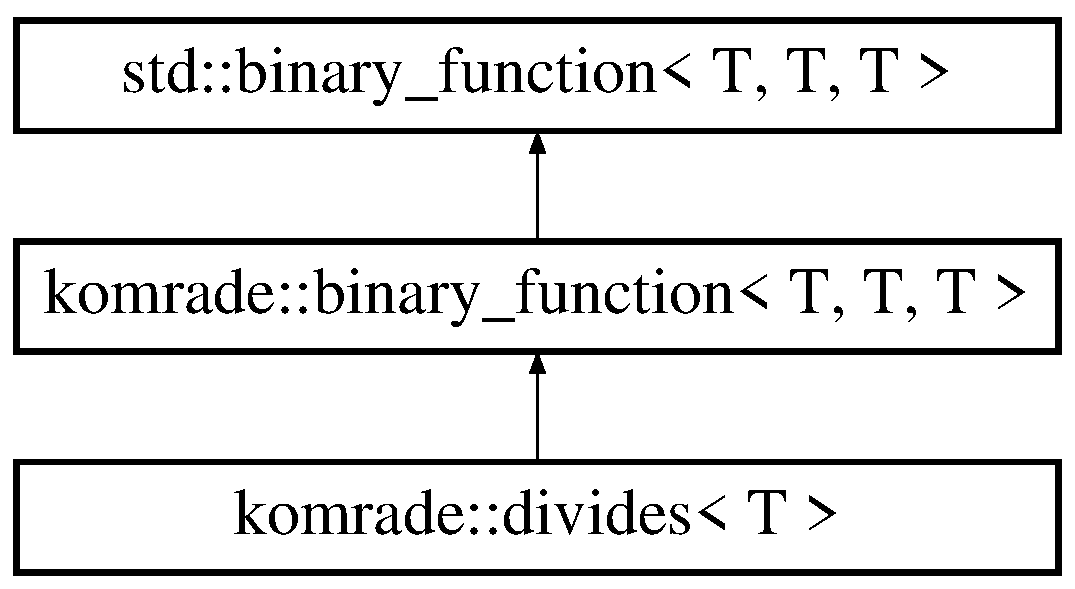
\includegraphics[height=3cm]{structkomrade_1_1divides}
\end{center}
\end{figure}
\subsection*{Public Member Functions}
\begin{CompactItemize}
\item 
\_\-\_\-host\_\-\_\- \_\-\_\-device\_\-\_\- T {\bf operator()} (const T \&lhs, const T \&rhs) const 
\end{CompactItemize}


\subsection{Detailed Description}
\subsubsection*{template$<$typename T$>$ struct komrade::divides$<$ T $>$}

{\tt \doxyref{divides}{p.}{structkomrade_1_1divides}} is a function object. Specifically, it is an Adaptable Binary Function. If {\tt f} is an object of class {\tt divides$<$T$>$}, and {\tt x} and {\tt y} are objects of class {\tt T}, then {\tt f(x,y)} returns {\tt x/y}.

\begin{Desc}
\item[Template Parameters:]
\begin{description}
\item[{\em T}]is a model of {\tt Assignable}, and if {\tt x} and {\tt y} are objects of type {\tt T}, then {\tt x/y} must be defined and must have a return type that is convertible to {\tt T}.\end{description}
\end{Desc}
The following code snippet demonstrates how to use {\tt \doxyref{divides}{p.}{structkomrade_1_1divides}} to divide one device\_\-vectors of {\tt floats} by another.



\begin{Code}\begin{verbatim}  #include <komrade/device_vector.h>
  #include <komrade/functional.h>
  #include <komrade/range.h>
  #include <komrade/fill.h>
  #include <komrade/transform.h>
  ...
  const int N = 1000;
  komrade::device_vector<float> V1(N);
  komrade::device_vector<float> V2(N);
  komrade::device_vector<float> V3(N);

  komrade::range(V1.begin(), V1.end(), 1);
  komrade::fill(V2.begin(), V2.end(), 75);

  komrade::transform(V1.begin(), V1.end(), V2.begin(), V3.begin(),
                     komrade::divides<float>());
  // V3 is now {1/75, 2/75, 3/75, ..., 1000/75}
\end{verbatim}
\end{Code}



\begin{Desc}
\item[See also:]{\tt http://www.sgi.com/tech/stl/divides.html} 

\doxyref{binary\_\-function}{p.}{structkomrade_1_1binary__function} \end{Desc}


\subsection{Member Function Documentation}
\index{komrade::divides@{komrade::divides}!operator()@{operator()}}
\index{operator()@{operator()}!komrade::divides@{komrade::divides}}
\subsubsection[operator()]{\setlength{\rightskip}{0pt plus 5cm}template$<$typename T$>$ \_\-\_\-host\_\-\_\- \_\-\_\-device\_\-\_\- T {\bf komrade::divides}$<$ T $>$::operator() (const T \& {\em lhs}, \/  const T \& {\em rhs}) const\hspace{0.3cm}{\tt  [inline]}}\label{structkomrade_1_1divides_fe9b749d994594012b3f74549f61b321}


Function call operator. The return value is {\tt lhs / rhs}. 

The documentation for this struct was generated from the following file:\begin{CompactItemize}
\item 
{\bf functional.h}\end{CompactItemize}

\section{komrade::equal\_\-to$<$ T $>$ Struct Template Reference}
\label{structkomrade_1_1equal__to}\index{komrade::equal\_\-to@{komrade::equal\_\-to}}
{\tt \#include $<$functional.h$>$}

Inheritance diagram for komrade::equal\_\-to$<$ T $>$::\begin{figure}[H]
\begin{center}
\leavevmode
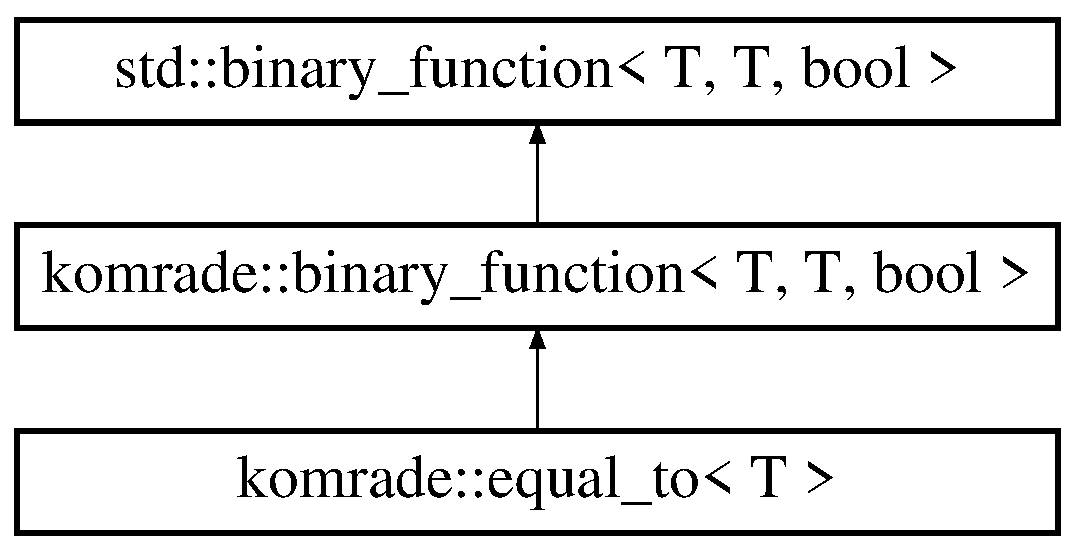
\includegraphics[height=3cm]{structkomrade_1_1equal__to}
\end{center}
\end{figure}
\subsection*{Public Member Functions}
\begin{CompactItemize}
\item 
\_\-\_\-host\_\-\_\- \_\-\_\-device\_\-\_\- bool {\bf operator()} (const T \&lhs, const T \&rhs) const 
\end{CompactItemize}


\subsection{Detailed Description}
\subsubsection*{template$<$typename T$>$ struct komrade::equal\_\-to$<$ T $>$}

{\tt \doxyref{equal\_\-to}{p.}{structkomrade_1_1equal__to}} is a function object. Specifically, it is an Adaptable Binary Predicate, which means it is a function object that tests the truth or falsehood of some condition. If {\tt f} is an object of class {\tt equal\_\-to$<$T$>$} and {\tt x} and {\tt y} are objects of class {\tt T}, then {\tt f(x,y)} returns {\tt true} if {\tt x == y} and {\tt false} otherwise.

\begin{Desc}
\item[Template Parameters:]
\begin{description}
\item[{\em T}]is a model of {\tt Equality Comparable}.\end{description}
\end{Desc}
\begin{Desc}
\item[See also:]{\tt http://www.sgi.com/tech/stl/equal\_\-to.html} 

\doxyref{binary\_\-function}{p.}{structkomrade_1_1binary__function} \end{Desc}


\subsection{Member Function Documentation}
\index{komrade::equal\_\-to@{komrade::equal\_\-to}!operator()@{operator()}}
\index{operator()@{operator()}!komrade::equal_to@{komrade::equal\_\-to}}
\subsubsection[operator()]{\setlength{\rightskip}{0pt plus 5cm}template$<$typename T$>$ \_\-\_\-host\_\-\_\- \_\-\_\-device\_\-\_\- bool {\bf komrade::equal\_\-to}$<$ T $>$::operator() (const T \& {\em lhs}, \/  const T \& {\em rhs}) const\hspace{0.3cm}{\tt  [inline]}}\label{structkomrade_1_1equal__to_51f3ffd68519667ac7eb28c93d205531}


Function call operator. The return value is {\tt lhs == rhs}. 

The documentation for this struct was generated from the following file:\begin{CompactItemize}
\item 
{\bf functional.h}\end{CompactItemize}

\section{komrade::forward\_\-device\_\-iterator\_\-tag Struct Reference}
\label{structkomrade_1_1forward__device__iterator__tag}\index{komrade::forward\_\-device\_\-iterator\_\-tag@{komrade::forward\_\-device\_\-iterator\_\-tag}}
{\tt \#include $<$iterator\_\-categories.h$>$}

Inheritance diagram for komrade::forward\_\-device\_\-iterator\_\-tag::\begin{figure}[H]
\begin{center}
\leavevmode
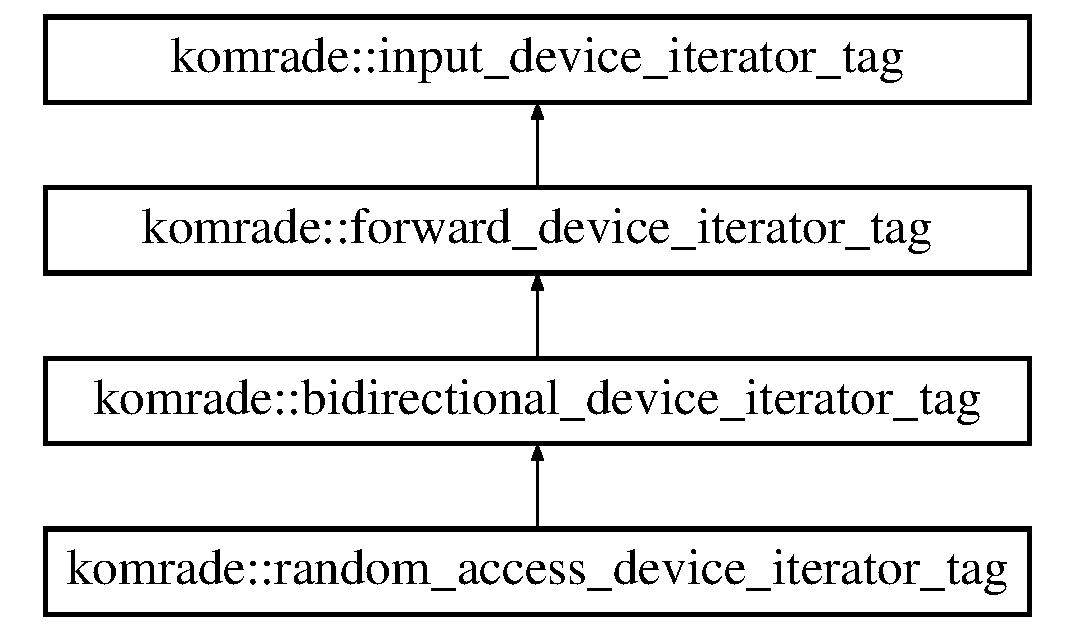
\includegraphics[height=4cm]{structkomrade_1_1forward__device__iterator__tag}
\end{center}
\end{figure}


\subsection{Detailed Description}
{\tt \doxyref{forward\_\-device\_\-iterator\_\-tag}{p.}{structkomrade_1_1forward__device__iterator__tag}} is an empty class: it has no member functions, member variables, or nested types. It is used solely as a \char`\"{}tag\char`\"{}: a representation of the Forward Device Iterator concept within the C++ type system.

\begin{Desc}
\item[See also:]{\tt http://www.sgi.com/tech/sgi/forward\_\-iterator\_\-tag.html,} iterator\_\-traits, \doxyref{input\_\-device\_\-iterator\_\-tag}{p.}{structkomrade_1_1input__device__iterator__tag}, \doxyref{output\_\-device\_\-iterator\_\-tag}{p.}{structkomrade_1_1output__device__iterator__tag}, \doxyref{bidirectional\_\-device\_\-iterator\_\-tag}{p.}{structkomrade_1_1bidirectional__device__iterator__tag}, \doxyref{random\_\-access\_\-device\_\-iterator\_\-tag}{p.}{structkomrade_1_1random__access__device__iterator__tag}, \doxyref{input\_\-host\_\-iterator\_\-tag}{p.}{group__iterator__tag__classes_g0927e3a6aecf64b535bd28052c7516d5}, \doxyref{output\_\-host\_\-iterator\_\-tag}{p.}{group__iterator__tag__classes_gba20a59557406e3ab657831abf6d65a0}, \doxyref{forward\_\-host\_\-iterator\_\-tag}{p.}{group__iterator__tag__classes_gc0af280b47824bd61134805db6ffe828}, \doxyref{bidirectional\_\-host\_\-iterator\_\-tag}{p.}{group__iterator__tag__classes_gbdabd9cb52934a67a931cfd93d6079f0}, \doxyref{random\_\-access\_\-host\_\-iterator\_\-tag}{p.}{group__iterator__tag__classes_gfde808d31f9339adeda3dcf88077da8d} \end{Desc}


The documentation for this struct was generated from the following file:\begin{CompactItemize}
\item 
{\bf iterator\_\-categories.h}\end{CompactItemize}

\section{komrade::greater$<$ T $>$ Struct Template Reference}
\label{structkomrade_1_1greater}\index{komrade::greater@{komrade::greater}}
{\tt \#include $<$functional.h$>$}

Inheritance diagram for komrade::greater$<$ T $>$::\begin{figure}[H]
\begin{center}
\leavevmode
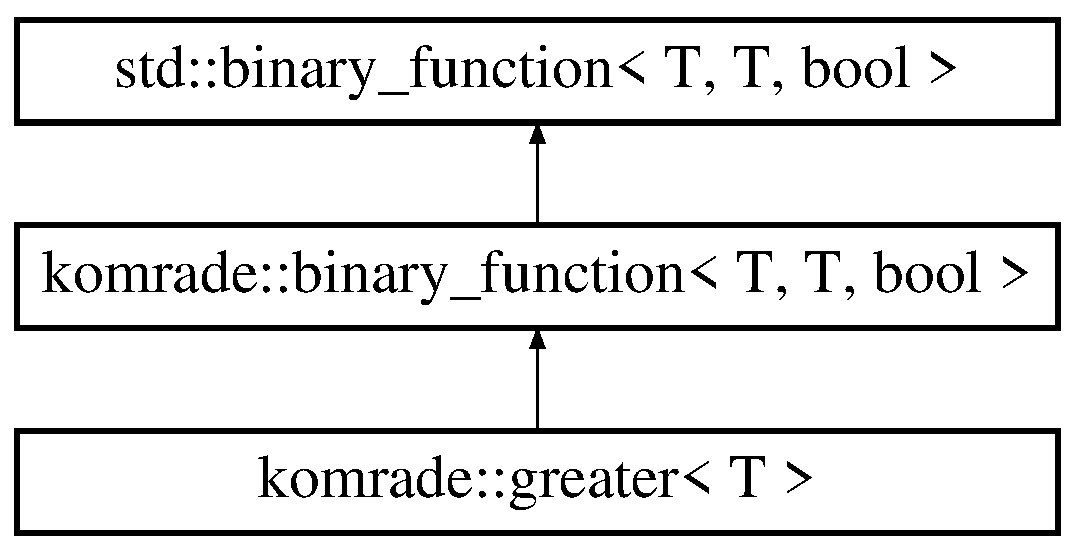
\includegraphics[height=3cm]{structkomrade_1_1greater}
\end{center}
\end{figure}
\subsection*{Public Member Functions}
\begin{CompactItemize}
\item 
\_\-\_\-host\_\-\_\- \_\-\_\-device\_\-\_\- bool {\bf operator()} (const T \&lhs, const T \&rhs) const 
\end{CompactItemize}


\subsection{Detailed Description}
\subsubsection*{template$<$typename T$>$ struct komrade::greater$<$ T $>$}

{\tt \doxyref{greater}{p.}{structkomrade_1_1greater}} is a function object. Specifically, it is an Adaptable Binary Predicate, which means it is a function object that tests the truth or falsehood of some condition. If {\tt f} is an object of class {\tt greater$<$T$>$} and {\tt x} and {\tt y} are objects of class {\tt T}, then {\tt f(x,y)} returns {\tt true} if {\tt x $>$ y} and {\tt false} otherwise.

\begin{Desc}
\item[Template Parameters:]
\begin{description}
\item[{\em T}]is a model of {\tt LessThan Comparable}.\end{description}
\end{Desc}
\begin{Desc}
\item[See also:]{\tt http://www.sgi.com/tech/stl/greater.html} 

\doxyref{binary\_\-function}{p.}{structkomrade_1_1binary__function} \end{Desc}


\subsection{Member Function Documentation}
\index{komrade::greater@{komrade::greater}!operator()@{operator()}}
\index{operator()@{operator()}!komrade::greater@{komrade::greater}}
\subsubsection[operator()]{\setlength{\rightskip}{0pt plus 5cm}template$<$typename T$>$ \_\-\_\-host\_\-\_\- \_\-\_\-device\_\-\_\- bool {\bf komrade::greater}$<$ T $>$::operator() (const T \& {\em lhs}, \/  const T \& {\em rhs}) const\hspace{0.3cm}{\tt  [inline]}}\label{structkomrade_1_1greater_2a590748d6deb69ac58d394c5968c1c1}


Function call operator. The return value is {\tt lhs $>$ rhs}. 

The documentation for this struct was generated from the following file:\begin{CompactItemize}
\item 
{\bf functional.h}\end{CompactItemize}

\section{komrade::greater\_\-equal$<$ T $>$ Struct Template Reference}
\label{structkomrade_1_1greater__equal}\index{komrade::greater\_\-equal@{komrade::greater\_\-equal}}
{\tt \#include $<$functional.h$>$}

Inheritance diagram for komrade::greater\_\-equal$<$ T $>$::\begin{figure}[H]
\begin{center}
\leavevmode
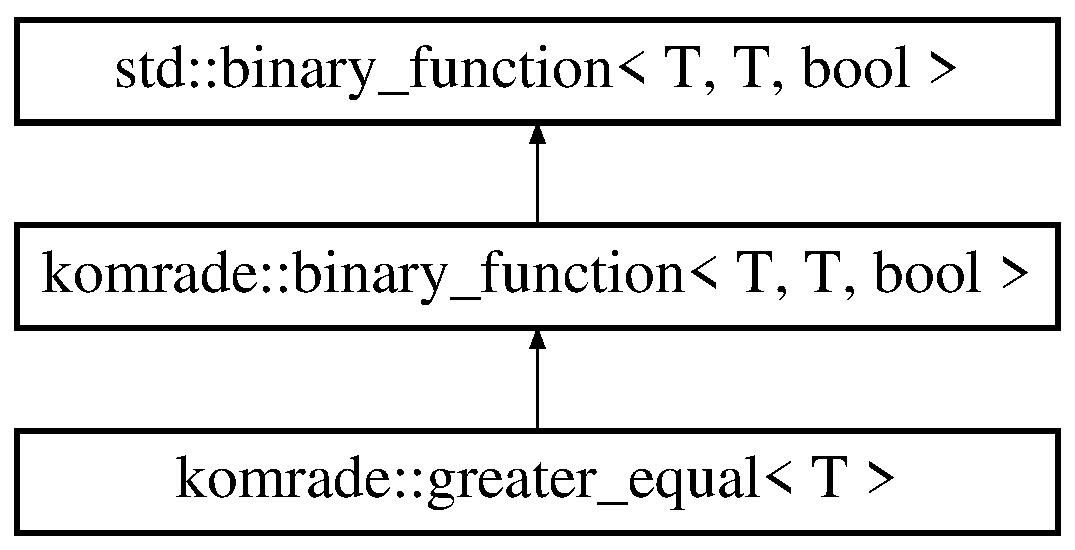
\includegraphics[height=3cm]{structkomrade_1_1greater__equal}
\end{center}
\end{figure}
\subsection*{Public Member Functions}
\begin{CompactItemize}
\item 
\_\-\_\-host\_\-\_\- \_\-\_\-device\_\-\_\- bool {\bf operator()} (const T \&lhs, const T \&rhs) const 
\end{CompactItemize}


\subsection{Detailed Description}
\subsubsection*{template$<$typename T$>$ struct komrade::greater\_\-equal$<$ T $>$}

{\tt \doxyref{greater\_\-equal}{p.}{structkomrade_1_1greater__equal}} is a function object. Specifically, it is an Adaptable Binary Predicate, which means it is a function object that tests the truth or falsehood of some condition. If {\tt f} is an object of class {\tt greater\_\-equal$<$T$>$} and {\tt x} and {\tt y} are objects of class {\tt T}, then {\tt f(x,y)} returns {\tt true} if {\tt x $>$= y} and {\tt false} otherwise.

\begin{Desc}
\item[Template Parameters:]
\begin{description}
\item[{\em T}]is a model of {\tt LessThan Comparable}.\end{description}
\end{Desc}
\begin{Desc}
\item[See also:]{\tt http://www.sgi.com/tech/stl/greater\_\-equal.html} 

\doxyref{binary\_\-function}{p.}{structkomrade_1_1binary__function} \end{Desc}


\subsection{Member Function Documentation}
\index{komrade::greater\_\-equal@{komrade::greater\_\-equal}!operator()@{operator()}}
\index{operator()@{operator()}!komrade::greater_equal@{komrade::greater\_\-equal}}
\subsubsection[operator()]{\setlength{\rightskip}{0pt plus 5cm}template$<$typename T$>$ \_\-\_\-host\_\-\_\- \_\-\_\-device\_\-\_\- bool {\bf komrade::greater\_\-equal}$<$ T $>$::operator() (const T \& {\em lhs}, \/  const T \& {\em rhs}) const\hspace{0.3cm}{\tt  [inline]}}\label{structkomrade_1_1greater__equal_8d86a4083502e297756ca776e03e1380}


Function call operator. The return value is {\tt lhs $>$= rhs}. 

The documentation for this struct was generated from the following file:\begin{CompactItemize}
\item 
{\bf functional.h}\end{CompactItemize}

\section{komrade::host\_\-vector$<$ T, Alloc $>$ Class Template Reference}
\label{classkomrade_1_1host__vector}\index{komrade::host\_\-vector@{komrade::host\_\-vector}}
{\tt \#include $<$host\_\-vector.h$>$}

\subsection*{Public Types}
\begin{CompactItemize}
\item 
typedef Parent::size\_\-type \textbf{size\_\-type}\label{classkomrade_1_1host__vector_73b176390d84ef97b48408608e3b2711}

\item 
typedef Parent::value\_\-type \textbf{value\_\-type}\label{classkomrade_1_1host__vector_24a9dddb392f08b0afe184067b7af9b4}

\end{CompactItemize}
\subsection*{Public Member Functions}
\begin{CompactItemize}
\item 
\_\-\_\-host\_\-\_\- {\bf host\_\-vector} (void)
\item 
\_\-\_\-host\_\-\_\- {\bf host\_\-vector} (size\_\-type n, const value\_\-type \&value=value\_\-type())
\item 
\_\-\_\-host\_\-\_\- {\bf host\_\-vector} (const {\bf host\_\-vector} \&v)
\item 
\_\-\_\-host\_\-\_\- {\bf host\_\-vector} \& {\bf operator=} (const {\bf host\_\-vector} \&v)
\item 
{\footnotesize template$<$typename OtherT, typename OtherAlloc$>$ }\\\_\-\_\-host\_\-\_\- {\bf host\_\-vector} (const {\bf host\_\-vector}$<$ OtherT, OtherAlloc $>$ \&v)
\item 
{\footnotesize template$<$typename OtherT, typename OtherAlloc$>$ }\\\_\-\_\-host\_\-\_\- {\bf host\_\-vector} \& {\bf operator=} (const {\bf host\_\-vector}$<$ OtherT, OtherAlloc $>$ \&v)
\item 
{\footnotesize template$<$typename OtherT, typename OtherAlloc$>$ }\\\_\-\_\-host\_\-\_\- {\bf host\_\-vector} (const std::vector$<$ OtherT, OtherAlloc $>$ \&v)
\item 
{\footnotesize template$<$typename OtherT, typename OtherAlloc$>$ }\\\_\-\_\-host\_\-\_\- {\bf host\_\-vector} \& {\bf operator=} (const std::vector$<$ OtherT, OtherAlloc $>$ \&v)
\item 
{\footnotesize template$<$typename OtherT, typename OtherAlloc$>$ }\\\_\-\_\-host\_\-\_\- {\bf host\_\-vector} (const {\bf device\_\-vector}$<$ OtherT, OtherAlloc $>$ \&v)
\item 
{\footnotesize template$<$typename InputIterator$>$ }\\\_\-\_\-host\_\-\_\- {\bf host\_\-vector} (InputIterator begin, InputIterator end)
\end{CompactItemize}


\subsection{Detailed Description}
\subsubsection*{template$<$typename T, typename Alloc = std::allocator$<$T$>$$>$ class komrade::host\_\-vector$<$ T, Alloc $>$}

A {\tt \doxyref{host\_\-vector}{p.}{classkomrade_1_1host__vector}} is a Host Sequence that supports random access to elements, constant time removal of elements at the end, and linear time insertion and removal of elements at the beginning or in the middle. The number of elements in a {\tt \doxyref{host\_\-vector}{p.}{classkomrade_1_1host__vector}} may vary dynamically; memory management is automatic. The memory associated with a {\tt \doxyref{host\_\-vector}{p.}{classkomrade_1_1host__vector}} resides in the memory space of the host associated with a parallel device.

Please refer to the {\tt C++ STL} for the documentation of {\tt host\_\-vector's} API.

\begin{Desc}
\item[See also:]{\tt http://www.sgi.com/tech/stl/Vector.html} 

\doxyref{device\_\-vector}{p.}{classkomrade_1_1device__vector}\end{Desc}
\begin{Desc}
\item[{\bf Bug}]The following members do not exist yet: {\tt reverse\_\-iterator}, {\tt const\_\-reverse\_\-iterator}, {\tt rbegin}, {\tt rend}, {\tt pop\_\-back}, {\tt insert}, {\tt operator$<$}.\end{Desc}


\subsection{Constructor \& Destructor Documentation}
\index{komrade::host\_\-vector@{komrade::host\_\-vector}!host\_\-vector@{host\_\-vector}}
\index{host\_\-vector@{host\_\-vector}!komrade::host_vector@{komrade::host\_\-vector}}
\subsubsection[host\_\-vector]{\setlength{\rightskip}{0pt plus 5cm}template$<$typename T, typename Alloc = std::allocator$<$T$>$$>$ \_\-\_\-host\_\-\_\- {\bf komrade::host\_\-vector}$<$ T, Alloc $>$::{\bf host\_\-vector} (void)\hspace{0.3cm}{\tt  [inline]}}\label{classkomrade_1_1host__vector_faf1218ac3a9aa5dd182d83086d8f996}


This constructor creates an empty {\tt \doxyref{host\_\-vector}{p.}{classkomrade_1_1host__vector}}. \index{komrade::host\_\-vector@{komrade::host\_\-vector}!host\_\-vector@{host\_\-vector}}
\index{host\_\-vector@{host\_\-vector}!komrade::host_vector@{komrade::host\_\-vector}}
\subsubsection[host\_\-vector]{\setlength{\rightskip}{0pt plus 5cm}template$<$typename T, typename Alloc = std::allocator$<$T$>$$>$ \_\-\_\-host\_\-\_\- {\bf komrade::host\_\-vector}$<$ T, Alloc $>$::{\bf host\_\-vector} (size\_\-type {\em n}, \/  const value\_\-type \& {\em value} = {\tt value\_\-type()})\hspace{0.3cm}{\tt  [inline, explicit]}}\label{classkomrade_1_1host__vector_1eaf269c6b5ee546c1add0f01e0c097d}


This constructor creates a {\tt \doxyref{host\_\-vector}{p.}{classkomrade_1_1host__vector}} with copies of an exemplar element. \begin{Desc}
\item[Parameters:]
\begin{description}
\item[{\em n}]The number of elements to initially create. \item[{\em value}]An element to copy. \end{description}
\end{Desc}
\index{komrade::host\_\-vector@{komrade::host\_\-vector}!host\_\-vector@{host\_\-vector}}
\index{host\_\-vector@{host\_\-vector}!komrade::host_vector@{komrade::host\_\-vector}}
\subsubsection[host\_\-vector]{\setlength{\rightskip}{0pt plus 5cm}template$<$typename T, typename Alloc = std::allocator$<$T$>$$>$ \_\-\_\-host\_\-\_\- {\bf komrade::host\_\-vector}$<$ T, Alloc $>$::{\bf host\_\-vector} (const {\bf host\_\-vector}$<$ T, Alloc $>$ \& {\em v})\hspace{0.3cm}{\tt  [inline]}}\label{classkomrade_1_1host__vector_23c446eb08ff1db44ec5df0b8d9e1778}


Copy constructor copies from an exemplar {\tt \doxyref{host\_\-vector}{p.}{classkomrade_1_1host__vector}}. \begin{Desc}
\item[Parameters:]
\begin{description}
\item[{\em v}]The {\tt \doxyref{host\_\-vector}{p.}{classkomrade_1_1host__vector}} to copy. \end{description}
\end{Desc}
\index{komrade::host\_\-vector@{komrade::host\_\-vector}!host\_\-vector@{host\_\-vector}}
\index{host\_\-vector@{host\_\-vector}!komrade::host_vector@{komrade::host\_\-vector}}
\subsubsection[host\_\-vector]{\setlength{\rightskip}{0pt plus 5cm}template$<$typename T, typename Alloc = std::allocator$<$T$>$$>$ template$<$typename OtherT, typename OtherAlloc$>$ \_\-\_\-host\_\-\_\- {\bf komrade::host\_\-vector}$<$ T, Alloc $>$::{\bf host\_\-vector} (const {\bf host\_\-vector}$<$ OtherT, OtherAlloc $>$ \& {\em v})\hspace{0.3cm}{\tt  [inline]}}\label{classkomrade_1_1host__vector_237ce62fb7d285a523d1e0678a8c9b76}


Copy constructor copies from an exemplar {\tt \doxyref{host\_\-vector}{p.}{classkomrade_1_1host__vector}} with different type. \begin{Desc}
\item[Parameters:]
\begin{description}
\item[{\em v}]The {\tt \doxyref{host\_\-vector}{p.}{classkomrade_1_1host__vector}} to copy. \end{description}
\end{Desc}
\index{komrade::host\_\-vector@{komrade::host\_\-vector}!host\_\-vector@{host\_\-vector}}
\index{host\_\-vector@{host\_\-vector}!komrade::host_vector@{komrade::host\_\-vector}}
\subsubsection[host\_\-vector]{\setlength{\rightskip}{0pt plus 5cm}template$<$typename T, typename Alloc = std::allocator$<$T$>$$>$ template$<$typename OtherT, typename OtherAlloc$>$ \_\-\_\-host\_\-\_\- {\bf komrade::host\_\-vector}$<$ T, Alloc $>$::{\bf host\_\-vector} (const std::vector$<$ OtherT, OtherAlloc $>$ \& {\em v})\hspace{0.3cm}{\tt  [inline]}}\label{classkomrade_1_1host__vector_60578fc4ed1e602bb7c7dc4171b2e3ad}


Copy constructor copies from an exemplar {\tt std::vector}. \begin{Desc}
\item[Parameters:]
\begin{description}
\item[{\em v}]The {\tt std::vector} to copy. \end{description}
\end{Desc}
\index{komrade::host\_\-vector@{komrade::host\_\-vector}!host\_\-vector@{host\_\-vector}}
\index{host\_\-vector@{host\_\-vector}!komrade::host_vector@{komrade::host\_\-vector}}
\subsubsection[host\_\-vector]{\setlength{\rightskip}{0pt plus 5cm}template$<$typename T, typename Alloc = std::allocator$<$T$>$$>$ template$<$typename OtherT, typename OtherAlloc$>$ \_\-\_\-host\_\-\_\- {\bf komrade::host\_\-vector}$<$ T, Alloc $>$::{\bf host\_\-vector} (const {\bf device\_\-vector}$<$ OtherT, OtherAlloc $>$ \& {\em v})\hspace{0.3cm}{\tt  [inline]}}\label{classkomrade_1_1host__vector_13d58e21be3962532696972320f68684}


Copy constructor copies from an exemplar {\tt \doxyref{device\_\-vector}{p.}{classkomrade_1_1device__vector}} with possibly different type. \begin{Desc}
\item[Parameters:]
\begin{description}
\item[{\em v}]The {\tt \doxyref{device\_\-vector}{p.}{classkomrade_1_1device__vector}} to copy. \end{description}
\end{Desc}
\index{komrade::host\_\-vector@{komrade::host\_\-vector}!host\_\-vector@{host\_\-vector}}
\index{host\_\-vector@{host\_\-vector}!komrade::host_vector@{komrade::host\_\-vector}}
\subsubsection[host\_\-vector]{\setlength{\rightskip}{0pt plus 5cm}template$<$typename T, typename Alloc = std::allocator$<$T$>$$>$ template$<$typename InputIterator$>$ \_\-\_\-host\_\-\_\- {\bf komrade::host\_\-vector}$<$ T, Alloc $>$::{\bf host\_\-vector} (InputIterator {\em begin}, \/  InputIterator {\em end})\hspace{0.3cm}{\tt  [inline]}}\label{classkomrade_1_1host__vector_3a2fc8f92f2dc60c2c2c01381aa186fe}


This constructor builds a {\tt \doxyref{host\_\-vector}{p.}{classkomrade_1_1host__vector}} from a range. \begin{Desc}
\item[Parameters:]
\begin{description}
\item[{\em begin}]The beginning of the range. \item[{\em end}]The end of the range. \end{description}
\end{Desc}


\subsection{Member Function Documentation}
\index{komrade::host\_\-vector@{komrade::host\_\-vector}!operator=@{operator=}}
\index{operator=@{operator=}!komrade::host_vector@{komrade::host\_\-vector}}
\subsubsection[operator=]{\setlength{\rightskip}{0pt plus 5cm}template$<$typename T, typename Alloc = std::allocator$<$T$>$$>$ \_\-\_\-host\_\-\_\- {\bf host\_\-vector}\& {\bf komrade::host\_\-vector}$<$ T, Alloc $>$::operator= (const {\bf host\_\-vector}$<$ T, Alloc $>$ \& {\em v})\hspace{0.3cm}{\tt  [inline]}}\label{classkomrade_1_1host__vector_7d6d8df547649787781d525181c14761}


Assign operator copies from an exemplar {\tt \doxyref{host\_\-vector}{p.}{classkomrade_1_1host__vector}}. \begin{Desc}
\item[Parameters:]
\begin{description}
\item[{\em v}]The {\tt \doxyref{host\_\-vector}{p.}{classkomrade_1_1host__vector}} to copy. \end{description}
\end{Desc}
\index{komrade::host\_\-vector@{komrade::host\_\-vector}!operator=@{operator=}}
\index{operator=@{operator=}!komrade::host_vector@{komrade::host\_\-vector}}
\subsubsection[operator=]{\setlength{\rightskip}{0pt plus 5cm}template$<$typename T, typename Alloc = std::allocator$<$T$>$$>$ template$<$typename OtherT, typename OtherAlloc$>$ \_\-\_\-host\_\-\_\- {\bf host\_\-vector}\& {\bf komrade::host\_\-vector}$<$ T, Alloc $>$::operator= (const {\bf host\_\-vector}$<$ OtherT, OtherAlloc $>$ \& {\em v})\hspace{0.3cm}{\tt  [inline]}}\label{classkomrade_1_1host__vector_dfc4858db8bb498f8501b5b44d4df128}


Assign operator copies from an exemplar {\tt \doxyref{host\_\-vector}{p.}{classkomrade_1_1host__vector}} with different type. \begin{Desc}
\item[Parameters:]
\begin{description}
\item[{\em v}]The {\tt \doxyref{host\_\-vector}{p.}{classkomrade_1_1host__vector}} to copy. \end{description}
\end{Desc}
\index{komrade::host\_\-vector@{komrade::host\_\-vector}!operator=@{operator=}}
\index{operator=@{operator=}!komrade::host_vector@{komrade::host\_\-vector}}
\subsubsection[operator=]{\setlength{\rightskip}{0pt plus 5cm}template$<$typename T, typename Alloc = std::allocator$<$T$>$$>$ template$<$typename OtherT, typename OtherAlloc$>$ \_\-\_\-host\_\-\_\- {\bf host\_\-vector}\& {\bf komrade::host\_\-vector}$<$ T, Alloc $>$::operator= (const std::vector$<$ OtherT, OtherAlloc $>$ \& {\em v})\hspace{0.3cm}{\tt  [inline]}}\label{classkomrade_1_1host__vector_eacdb16f803177e6171389c7b8fe46df}


Assign operator copies from an exemplar {\tt std::vector}. \begin{Desc}
\item[Parameters:]
\begin{description}
\item[{\em v}]The {\tt std::vector} to copy. \end{description}
\end{Desc}


The documentation for this class was generated from the following file:\begin{CompactItemize}
\item 
{\bf host\_\-vector.h}\end{CompactItemize}

\section{komrade::identity$<$ T $>$ Struct Template Reference}
\label{structkomrade_1_1identity}\index{komrade::identity@{komrade::identity}}
{\tt \#include $<$functional.h$>$}

Inheritance diagram for komrade::identity$<$ T $>$::\begin{figure}[H]
\begin{center}
\leavevmode
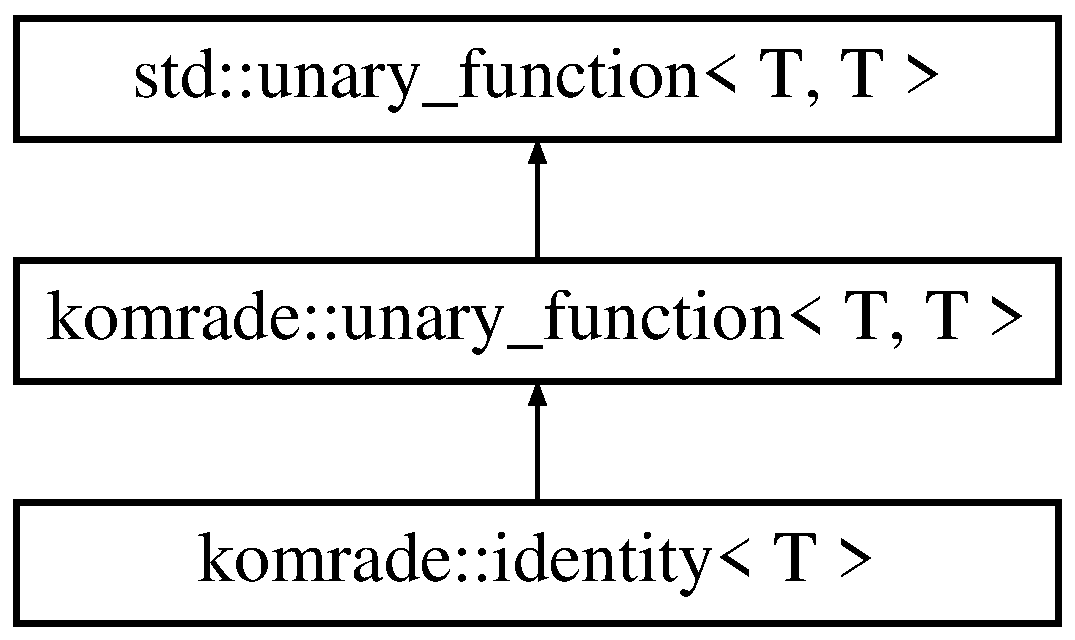
\includegraphics[height=3cm]{structkomrade_1_1identity}
\end{center}
\end{figure}
\subsection*{Public Member Functions}
\begin{CompactItemize}
\item 
\_\-\_\-host\_\-\_\- \_\-\_\-device\_\-\_\- T {\bf operator()} (const T \&x) const 
\end{CompactItemize}


\subsection{Detailed Description}
\subsubsection*{template$<$typename T$>$ struct komrade::identity$<$ T $>$}

{\tt \doxyref{identity}{p.}{structkomrade_1_1identity}} is a Unary Function that represents the \doxyref{identity}{p.}{structkomrade_1_1identity} function: it takes a single argument {\tt x}, and returns {\tt x}.

\begin{Desc}
\item[Template Parameters:]
\begin{description}
\item[{\em T}]No requirements on {\tt T}.\end{description}
\end{Desc}
The following code snippet demonstrates that {\tt \doxyref{identity}{p.}{structkomrade_1_1identity}} returns its argument.



\begin{Code}\begin{verbatim}  #include <komrade/functional.h>
  #include <assert.h>
  ...
  int x = 137;
  komrade::identity<int> id;
  assert(x == id(x));
\end{verbatim}
\end{Code}



\begin{Desc}
\item[See also:]{\tt http://www.sgi.com/tech/stl/identity.html} 

\doxyref{unary\_\-function}{p.}{structkomrade_1_1unary__function} \end{Desc}


\subsection{Member Function Documentation}
\index{komrade::identity@{komrade::identity}!operator()@{operator()}}
\index{operator()@{operator()}!komrade::identity@{komrade::identity}}
\subsubsection[operator()]{\setlength{\rightskip}{0pt plus 5cm}template$<$typename T$>$ \_\-\_\-host\_\-\_\- \_\-\_\-device\_\-\_\- T {\bf komrade::identity}$<$ T $>$::operator() (const T \& {\em x}) const\hspace{0.3cm}{\tt  [inline]}}\label{structkomrade_1_1identity_4527c0a73f266f53d648bb3de003015c}


Function call operator. The return value is {\tt x}. \begin{Desc}
\item[{\bf Bug}]identity$<$T$>$::operator()() should return const T \& \end{Desc}


The documentation for this struct was generated from the following file:\begin{CompactItemize}
\item 
{\bf functional.h}\end{CompactItemize}

\section{komrade::input\_\-device\_\-iterator\_\-tag Struct Reference}
\label{structkomrade_1_1input__device__iterator__tag}\index{komrade::input\_\-device\_\-iterator\_\-tag@{komrade::input\_\-device\_\-iterator\_\-tag}}
{\tt \#include $<$iterator\_\-categories.h$>$}

Inheritance diagram for komrade::input\_\-device\_\-iterator\_\-tag::\begin{figure}[H]
\begin{center}
\leavevmode
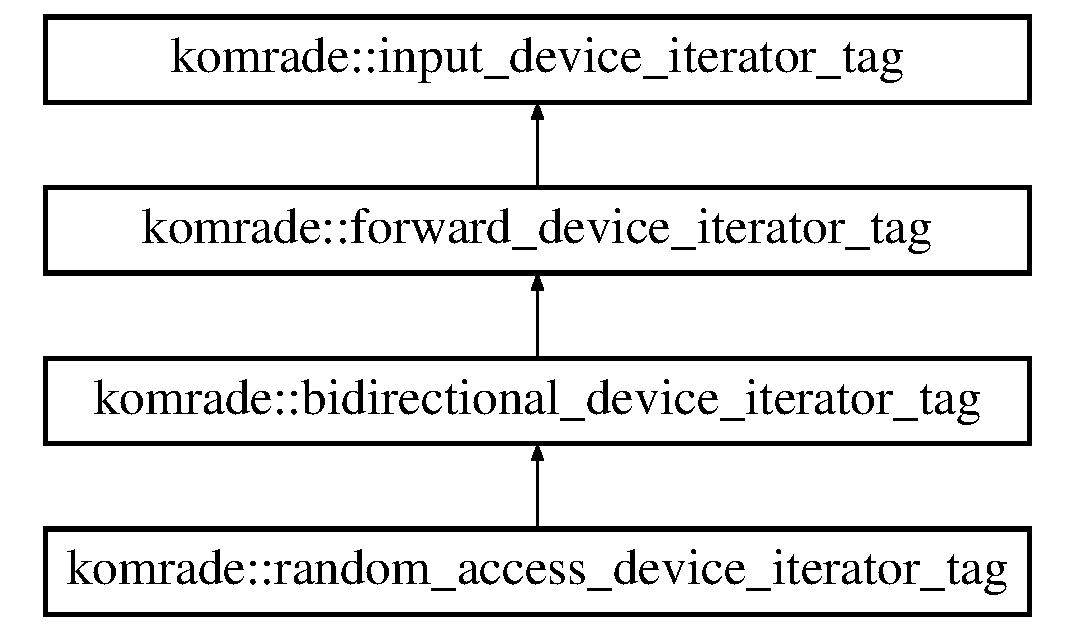
\includegraphics[height=4cm]{structkomrade_1_1input__device__iterator__tag}
\end{center}
\end{figure}


\subsection{Detailed Description}
{\tt \doxyref{input\_\-device\_\-iterator\_\-tag}{p.}{structkomrade_1_1input__device__iterator__tag}} is an empty class: it has no member functions, member variables, or nested types. It is used solely as a \char`\"{}tag\char`\"{}: a representation of the Input Device Iterator concept within the C++ type system.

\begin{Desc}
\item[See also:]{\tt http://www.sgi.com/tech/sgi/input\_\-iterator\_\-tag.html,} iterator\_\-traits, \doxyref{output\_\-device\_\-iterator\_\-tag}{p.}{structkomrade_1_1output__device__iterator__tag}, \doxyref{forward\_\-device\_\-iterator\_\-tag}{p.}{structkomrade_1_1forward__device__iterator__tag}, \doxyref{bidirectional\_\-device\_\-iterator\_\-tag}{p.}{structkomrade_1_1bidirectional__device__iterator__tag}, \doxyref{random\_\-access\_\-device\_\-iterator\_\-tag}{p.}{structkomrade_1_1random__access__device__iterator__tag}, \doxyref{input\_\-host\_\-iterator\_\-tag}{p.}{group__iterator__tag__classes_g0927e3a6aecf64b535bd28052c7516d5}, \doxyref{output\_\-host\_\-iterator\_\-tag}{p.}{group__iterator__tag__classes_gba20a59557406e3ab657831abf6d65a0}, \doxyref{forward\_\-host\_\-iterator\_\-tag}{p.}{group__iterator__tag__classes_gc0af280b47824bd61134805db6ffe828}, \doxyref{bidirectional\_\-host\_\-iterator\_\-tag}{p.}{group__iterator__tag__classes_gbdabd9cb52934a67a931cfd93d6079f0}, \doxyref{random\_\-access\_\-host\_\-iterator\_\-tag}{p.}{group__iterator__tag__classes_gfde808d31f9339adeda3dcf88077da8d} \end{Desc}


The documentation for this struct was generated from the following file:\begin{CompactItemize}
\item 
{\bf iterator\_\-categories.h}\end{CompactItemize}

\section{komrade::less$<$ T $>$ Struct Template Reference}
\label{structkomrade_1_1less}\index{komrade::less@{komrade::less}}
{\tt \#include $<$functional.h$>$}

Inheritance diagram for komrade::less$<$ T $>$::\begin{figure}[H]
\begin{center}
\leavevmode
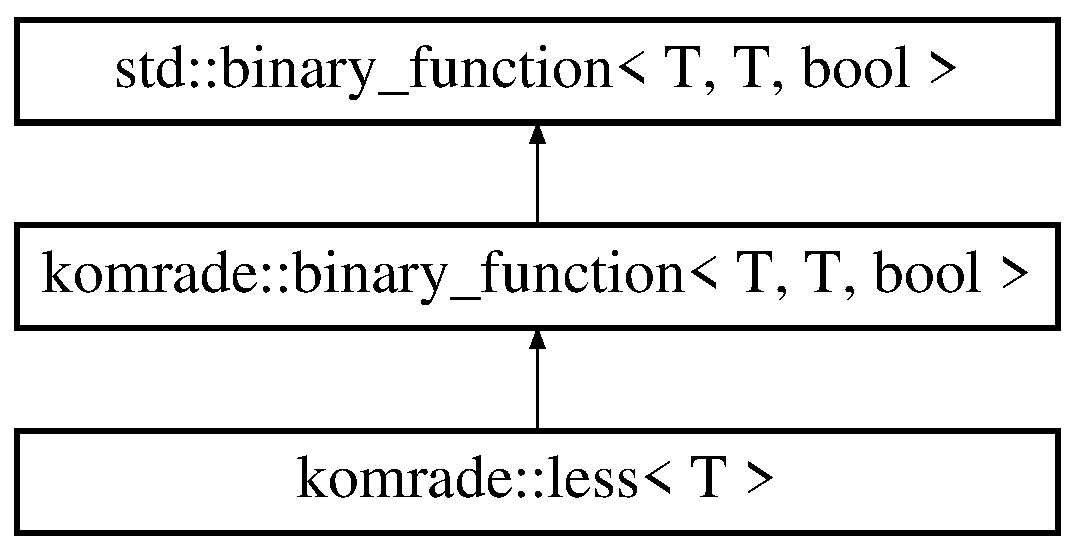
\includegraphics[height=3cm]{structkomrade_1_1less}
\end{center}
\end{figure}
\subsection*{Public Member Functions}
\begin{CompactItemize}
\item 
\_\-\_\-host\_\-\_\- \_\-\_\-device\_\-\_\- bool {\bf operator()} (const T \&lhs, const T \&rhs) const 
\end{CompactItemize}


\subsection{Detailed Description}
\subsubsection*{template$<$typename T$>$ struct komrade::less$<$ T $>$}

{\tt \doxyref{less}{p.}{structkomrade_1_1less}} is a function object. Specifically, it is an Adaptable Binary Predicate, which means it is a function object that tests the truth or falsehood of some condition. If {\tt f} is an object of class {\tt less$<$T$>$} and {\tt x} and {\tt y} are objects of class {\tt T}, then {\tt f(x,y)} returns {\tt true} if {\tt x $<$ y} and {\tt false} otherwise.

\begin{Desc}
\item[Template Parameters:]
\begin{description}
\item[{\em T}]is a model of {\tt LessThan Comparable}.\end{description}
\end{Desc}
\begin{Desc}
\item[See also:]{\tt http://www.sgi.com/tech/stl/less.html} 

\doxyref{binary\_\-function}{p.}{structkomrade_1_1binary__function} \end{Desc}


\subsection{Member Function Documentation}
\index{komrade::less@{komrade::less}!operator()@{operator()}}
\index{operator()@{operator()}!komrade::less@{komrade::less}}
\subsubsection[operator()]{\setlength{\rightskip}{0pt plus 5cm}template$<$typename T$>$ \_\-\_\-host\_\-\_\- \_\-\_\-device\_\-\_\- bool {\bf komrade::less}$<$ T $>$::operator() (const T \& {\em lhs}, \/  const T \& {\em rhs}) const\hspace{0.3cm}{\tt  [inline]}}\label{structkomrade_1_1less_ea2b67ce0094dcded73f2178e24df087}


Function call operator. The return value is {\tt lhs $<$ rhs}. 

The documentation for this struct was generated from the following file:\begin{CompactItemize}
\item 
{\bf functional.h}\end{CompactItemize}

\section{komrade::less\_\-equal$<$ T $>$ Struct Template Reference}
\label{structkomrade_1_1less__equal}\index{komrade::less\_\-equal@{komrade::less\_\-equal}}
{\tt \#include $<$functional.h$>$}

Inheritance diagram for komrade::less\_\-equal$<$ T $>$::\begin{figure}[H]
\begin{center}
\leavevmode
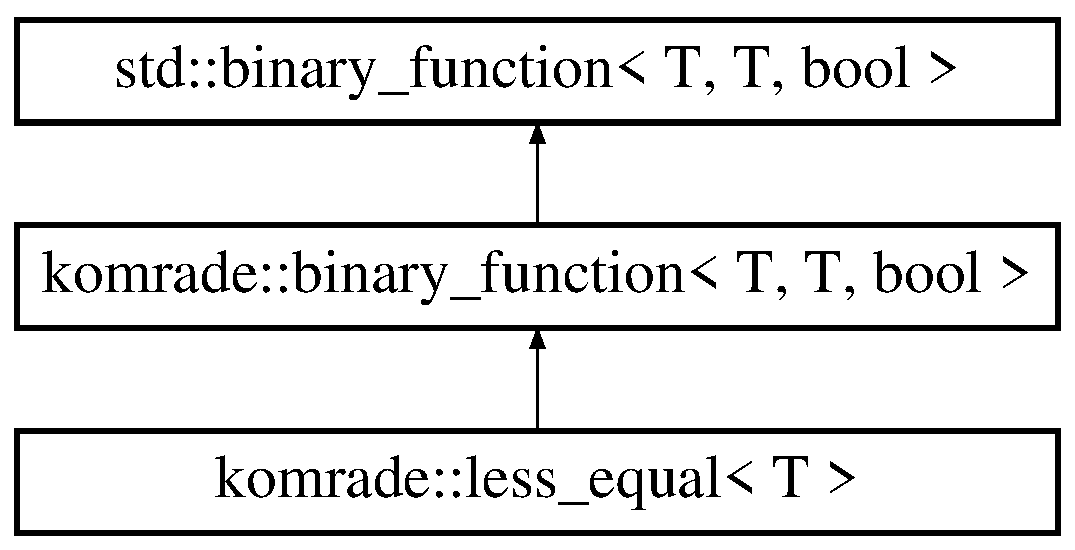
\includegraphics[height=3cm]{structkomrade_1_1less__equal}
\end{center}
\end{figure}
\subsection*{Public Member Functions}
\begin{CompactItemize}
\item 
\_\-\_\-host\_\-\_\- \_\-\_\-device\_\-\_\- bool {\bf operator()} (const T \&lhs, const T \&rhs) const 
\end{CompactItemize}


\subsection{Detailed Description}
\subsubsection*{template$<$typename T$>$ struct komrade::less\_\-equal$<$ T $>$}

{\tt \doxyref{less\_\-equal}{p.}{structkomrade_1_1less__equal}} is a function object. Specifically, it is an Adaptable Binary Predicate, which means it is a function object that tests the truth or falsehood of some condition. If {\tt f} is an object of class {\tt less\_\-equal$<$T$>$} and {\tt x} and {\tt y} are objects of class {\tt T}, then {\tt f(x,y)} returns {\tt true} if {\tt x $<$= y} and {\tt false} otherwise.

\begin{Desc}
\item[Template Parameters:]
\begin{description}
\item[{\em T}]is a model of {\tt LessThan Comparable}.\end{description}
\end{Desc}
\begin{Desc}
\item[See also:]{\tt http://www.sgi.com/tech/stl/less\_\-equal.html} 

\doxyref{binary\_\-function}{p.}{structkomrade_1_1binary__function} \end{Desc}


\subsection{Member Function Documentation}
\index{komrade::less\_\-equal@{komrade::less\_\-equal}!operator()@{operator()}}
\index{operator()@{operator()}!komrade::less_equal@{komrade::less\_\-equal}}
\subsubsection[operator()]{\setlength{\rightskip}{0pt plus 5cm}template$<$typename T$>$ \_\-\_\-host\_\-\_\- \_\-\_\-device\_\-\_\- bool {\bf komrade::less\_\-equal}$<$ T $>$::operator() (const T \& {\em lhs}, \/  const T \& {\em rhs}) const\hspace{0.3cm}{\tt  [inline]}}\label{structkomrade_1_1less__equal_a77ca576e3e9727727c9200fdf9d6f05}


Function call operator. The return value is {\tt lhs $<$= rhs}. 

The documentation for this struct was generated from the following file:\begin{CompactItemize}
\item 
{\bf functional.h}\end{CompactItemize}

\section{komrade::logical\_\-and$<$ T $>$ Struct Template Reference}
\label{structkomrade_1_1logical__and}\index{komrade::logical\_\-and@{komrade::logical\_\-and}}
{\tt \#include $<$functional.h$>$}

Inheritance diagram for komrade::logical\_\-and$<$ T $>$::\begin{figure}[H]
\begin{center}
\leavevmode
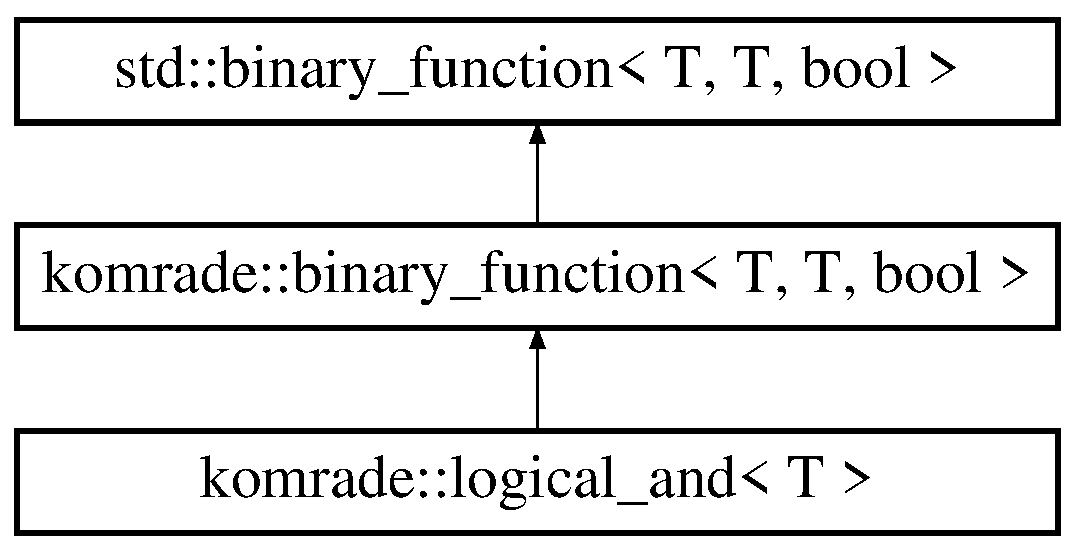
\includegraphics[height=3cm]{structkomrade_1_1logical__and}
\end{center}
\end{figure}
\subsection*{Public Member Functions}
\begin{CompactItemize}
\item 
\_\-\_\-host\_\-\_\- \_\-\_\-device\_\-\_\- bool {\bf operator()} (const T \&lhs, const T \&rhs) const 
\end{CompactItemize}


\subsection{Detailed Description}
\subsubsection*{template$<$typename T$>$ struct komrade::logical\_\-and$<$ T $>$}

{\tt \doxyref{logical\_\-and}{p.}{structkomrade_1_1logical__and}} is a function object. Specifically, it is an Adaptable Binary Predicate, which means it is a function object that tests the truth or falsehood of some condition. If {\tt f} is an object of class {\tt logical\_\-and$<$T$>$} and {\tt x} and {\tt y} are objects of class {\tt T} (where {\tt T} is convertible to {\tt bool}) then {\tt f(x,y)} returns {\tt true} if and only if both {\tt x} and {\tt y} are {\tt true}.

\begin{Desc}
\item[Template Parameters:]
\begin{description}
\item[{\em T}]must be convertible to {\tt bool}.\end{description}
\end{Desc}
\begin{Desc}
\item[See also:]{\tt http://www.sgi.com/tech/stl/logical\_\-and.html} 

\doxyref{binary\_\-function}{p.}{structkomrade_1_1binary__function} \end{Desc}


\subsection{Member Function Documentation}
\index{komrade::logical\_\-and@{komrade::logical\_\-and}!operator()@{operator()}}
\index{operator()@{operator()}!komrade::logical_and@{komrade::logical\_\-and}}
\subsubsection[operator()]{\setlength{\rightskip}{0pt plus 5cm}template$<$typename T$>$ \_\-\_\-host\_\-\_\- \_\-\_\-device\_\-\_\- bool {\bf komrade::logical\_\-and}$<$ T $>$::operator() (const T \& {\em lhs}, \/  const T \& {\em rhs}) const\hspace{0.3cm}{\tt  [inline]}}\label{structkomrade_1_1logical__and_a9ab2c7f0aaf17801df8871024d6b99a}


Function call operator. The return value is {\tt lhs \&\& rhs}. 

The documentation for this struct was generated from the following file:\begin{CompactItemize}
\item 
{\bf functional.h}\end{CompactItemize}

\section{komrade::logical\_\-not$<$ T $>$ Struct Template Reference}
\label{structkomrade_1_1logical__not}\index{komrade::logical\_\-not@{komrade::logical\_\-not}}
{\tt \#include $<$functional.h$>$}

Inheritance diagram for komrade::logical\_\-not$<$ T $>$::\begin{figure}[H]
\begin{center}
\leavevmode
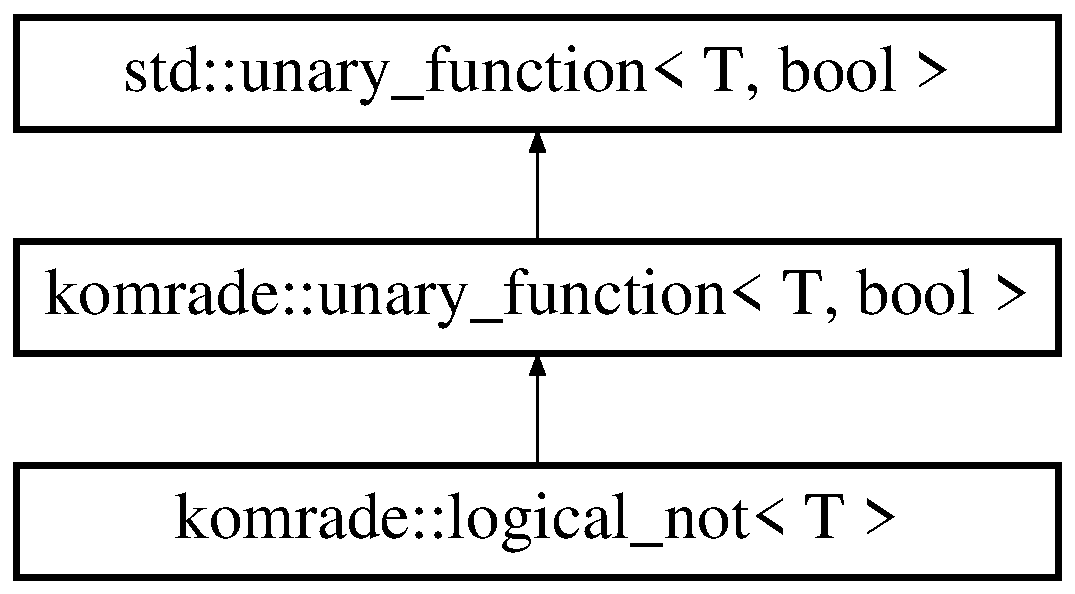
\includegraphics[height=3cm]{structkomrade_1_1logical__not}
\end{center}
\end{figure}
\subsection*{Public Member Functions}
\begin{CompactItemize}
\item 
\_\-\_\-host\_\-\_\- \_\-\_\-device\_\-\_\- bool {\bf operator()} (const T \&x) const 
\end{CompactItemize}


\subsection{Detailed Description}
\subsubsection*{template$<$typename T$>$ struct komrade::logical\_\-not$<$ T $>$}

{\tt \doxyref{logical\_\-not}{p.}{structkomrade_1_1logical__not}} is a function object. Specifically, it is an Adaptable Predicate, which means it is a function object that tests the truth or falsehood of some condition. If {\tt f} is an object of class {\tt logical\_\-not$<$T$>$} and {\tt x} is an object of class {\tt T} (where {\tt T} is convertible to {\tt bool}) then {\tt f(x)} returns {\tt true} if and only if {\tt x} is {\tt false}.

\begin{Desc}
\item[Template Parameters:]
\begin{description}
\item[{\em T}]must be convertible to {\tt bool}.\end{description}
\end{Desc}
The following code snippet demonstrates how to use {\tt \doxyref{logical\_\-not}{p.}{structkomrade_1_1logical__not}} to transform a \doxyref{device\_\-vector}{p.}{classkomrade_1_1device__vector} of {\tt bools} into its logical complement.



\begin{Code}\begin{verbatim}  #include <komrade/device_vector.h>
  #include <komrade/transform.h>
  #include <komrade/functional.h>
  ...
  komrade::device_vector<bool> V;
  ...
  komrade::transform(V.begin(), V.end(), V.begin(), komrade::logical_not<bool>());
  // The elements of V are now the logical complement of what they were prior
\end{verbatim}
\end{Code}



\begin{Desc}
\item[See also:]{\tt http://www.sgi.com/tech/stl/logical\_\-not.html} 

\doxyref{unary\_\-function}{p.}{structkomrade_1_1unary__function} \end{Desc}


\subsection{Member Function Documentation}
\index{komrade::logical\_\-not@{komrade::logical\_\-not}!operator()@{operator()}}
\index{operator()@{operator()}!komrade::logical_not@{komrade::logical\_\-not}}
\subsubsection[operator()]{\setlength{\rightskip}{0pt plus 5cm}template$<$typename T$>$ \_\-\_\-host\_\-\_\- \_\-\_\-device\_\-\_\- bool {\bf komrade::logical\_\-not}$<$ T $>$::operator() (const T \& {\em x}) const\hspace{0.3cm}{\tt  [inline]}}\label{structkomrade_1_1logical__not_d7e098d08b47bf62df8d56fbc295bb90}


Function call operator. The return value is {\tt !x}. 

The documentation for this struct was generated from the following file:\begin{CompactItemize}
\item 
{\bf functional.h}\end{CompactItemize}

\section{komrade::logical\_\-or$<$ T $>$ Struct Template Reference}
\label{structkomrade_1_1logical__or}\index{komrade::logical\_\-or@{komrade::logical\_\-or}}
{\tt \#include $<$functional.h$>$}

Inheritance diagram for komrade::logical\_\-or$<$ T $>$::\begin{figure}[H]
\begin{center}
\leavevmode
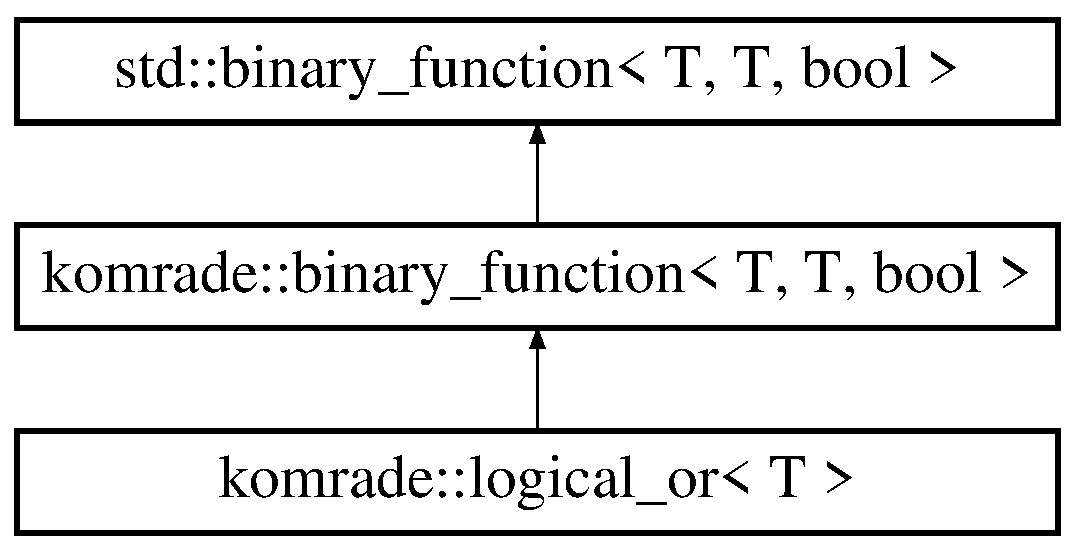
\includegraphics[height=3cm]{structkomrade_1_1logical__or}
\end{center}
\end{figure}
\subsection*{Public Member Functions}
\begin{CompactItemize}
\item 
\_\-\_\-host\_\-\_\- \_\-\_\-device\_\-\_\- bool {\bf operator()} (const T \&lhs, const T \&rhs) const 
\end{CompactItemize}


\subsection{Detailed Description}
\subsubsection*{template$<$typename T$>$ struct komrade::logical\_\-or$<$ T $>$}

{\tt \doxyref{logical\_\-or}{p.}{structkomrade_1_1logical__or}} is a function object. Specifically, it is an Adaptable Binary Predicate, which means it is a function object that tests the truth or falsehood of some condition. If {\tt f} is an object of class {\tt logical\_\-or$<$T$>$} and {\tt x} and {\tt y} are objects of class {\tt T} (where {\tt T} is convertible to {\tt bool}) then {\tt f(x,y)} returns {\tt true} if and only if either {\tt x} or {\tt y} are {\tt true}.

\begin{Desc}
\item[Template Parameters:]
\begin{description}
\item[{\em T}]must be convertible to {\tt bool}.\end{description}
\end{Desc}
\begin{Desc}
\item[See also:]{\tt http://www.sgi.com/tech/stl/logical\_\-or.html} 

\doxyref{binary\_\-function}{p.}{structkomrade_1_1binary__function} \end{Desc}


\subsection{Member Function Documentation}
\index{komrade::logical\_\-or@{komrade::logical\_\-or}!operator()@{operator()}}
\index{operator()@{operator()}!komrade::logical_or@{komrade::logical\_\-or}}
\subsubsection[operator()]{\setlength{\rightskip}{0pt plus 5cm}template$<$typename T$>$ \_\-\_\-host\_\-\_\- \_\-\_\-device\_\-\_\- bool {\bf komrade::logical\_\-or}$<$ T $>$::operator() (const T \& {\em lhs}, \/  const T \& {\em rhs}) const\hspace{0.3cm}{\tt  [inline]}}\label{structkomrade_1_1logical__or_f9ab6955831eab6c3cd416f6f1dcbe69}


Function call operator. The return value is {\tt lhs $|$$|$ rhs}. 

The documentation for this struct was generated from the following file:\begin{CompactItemize}
\item 
{\bf functional.h}\end{CompactItemize}

\section{komrade::maximum$<$ T $>$ Struct Template Reference}
\label{structkomrade_1_1maximum}\index{komrade::maximum@{komrade::maximum}}
{\tt \#include $<$functional.h$>$}

Inheritance diagram for komrade::maximum$<$ T $>$::\begin{figure}[H]
\begin{center}
\leavevmode
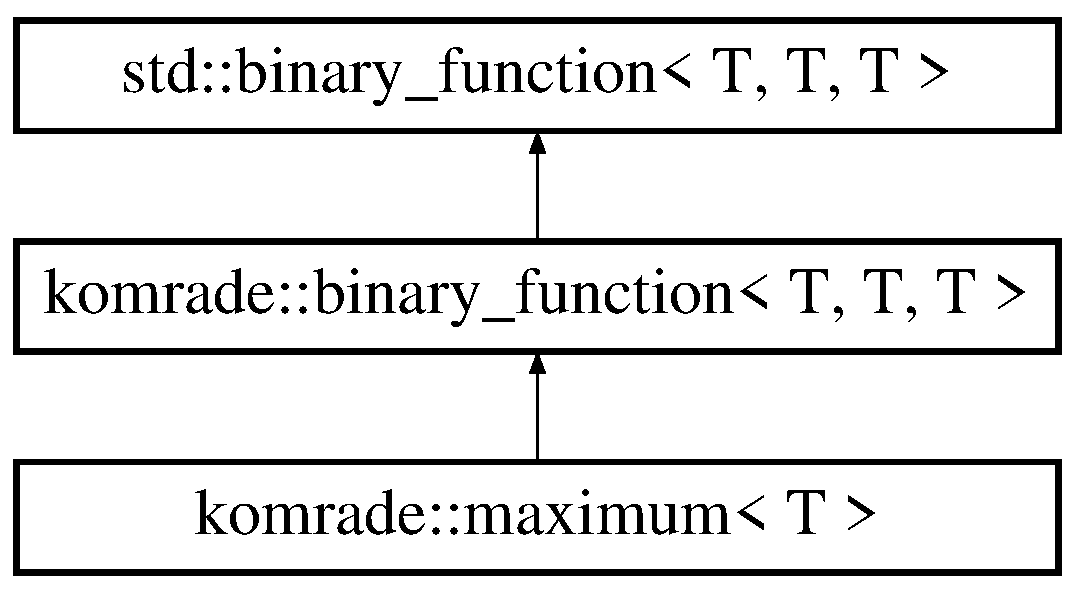
\includegraphics[height=3cm]{structkomrade_1_1maximum}
\end{center}
\end{figure}
\subsection*{Public Member Functions}
\begin{CompactItemize}
\item 
\_\-\_\-host\_\-\_\- \_\-\_\-device\_\-\_\- T {\bf operator()} (const T \&lhs, const T \&rhs) const 
\end{CompactItemize}


\subsection{Detailed Description}
\subsubsection*{template$<$typename T$>$ struct komrade::maximum$<$ T $>$}

{\tt \doxyref{maximum}{p.}{structkomrade_1_1maximum}} is a function object that takes two arguments and returns the \doxyref{greater}{p.}{structkomrade_1_1greater} of the two. Specifically, it is an Adaptable Binary Function. If {\tt f} is an object of class {\tt maximum$<$T$>$} and {\tt x} and {\tt y} are objects of class {\tt T} {\tt f(x,y)} returns {\tt x} if {\tt x $>$ y} and {\tt y}, otherwise.

\begin{Desc}
\item[Template Parameters:]
\begin{description}
\item[{\em T}]is a model of {\tt LessThan Comparable}.\end{description}
\end{Desc}
The following code snippet demonstrates that {\tt \doxyref{maximum}{p.}{structkomrade_1_1maximum}} returns its \doxyref{greater}{p.}{structkomrade_1_1greater} argument.



\begin{Code}\begin{verbatim}  #include <komrade/functional.h>
  #include <assert.h>
  ...
  int x =  137;
  int y = -137;
  komrade::maximum<int> mx;
  assert(x == mx(x,y));
\end{verbatim}
\end{Code}



\begin{Desc}
\item[See also:]\doxyref{minimum}{p.}{structkomrade_1_1minimum} 

\doxyref{min}{p.}{namespacekomrade_00a10d45e81d2110b8a79dbfb7ef3e9b} 

\doxyref{binary\_\-function}{p.}{structkomrade_1_1binary__function} \end{Desc}


\subsection{Member Function Documentation}
\index{komrade::maximum@{komrade::maximum}!operator()@{operator()}}
\index{operator()@{operator()}!komrade::maximum@{komrade::maximum}}
\subsubsection[operator()]{\setlength{\rightskip}{0pt plus 5cm}template$<$typename T$>$ \_\-\_\-host\_\-\_\- \_\-\_\-device\_\-\_\- T {\bf komrade::maximum}$<$ T $>$::operator() (const T \& {\em lhs}, \/  const T \& {\em rhs}) const\hspace{0.3cm}{\tt  [inline]}}\label{structkomrade_1_1maximum_eb1525b1d85bd295a8fba952c32f3233}


Function call operator. The return value is {\tt lhs $>$ rhs ? lhs : rhs}. \begin{Desc}
\item[{\bf Bug}]maximum$<$T$>$::operator()() should return const T \& \end{Desc}


The documentation for this struct was generated from the following file:\begin{CompactItemize}
\item 
{\bf functional.h}\end{CompactItemize}

\section{komrade::minimum$<$ T $>$ Struct Template Reference}
\label{structkomrade_1_1minimum}\index{komrade::minimum@{komrade::minimum}}
{\tt \#include $<$functional.h$>$}

Inheritance diagram for komrade::minimum$<$ T $>$::\begin{figure}[H]
\begin{center}
\leavevmode
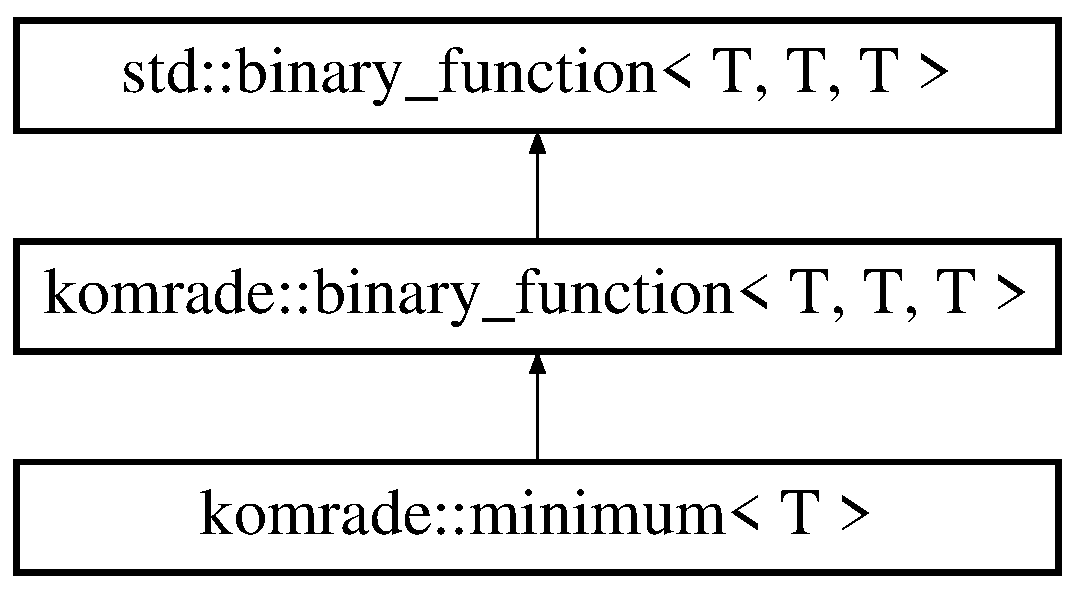
\includegraphics[height=3cm]{structkomrade_1_1minimum}
\end{center}
\end{figure}
\subsection*{Public Member Functions}
\begin{CompactItemize}
\item 
\_\-\_\-host\_\-\_\- \_\-\_\-device\_\-\_\- T {\bf operator()} (const T \&lhs, const T \&rhs) const 
\end{CompactItemize}


\subsection{Detailed Description}
\subsubsection*{template$<$typename T$>$ struct komrade::minimum$<$ T $>$}

{\tt \doxyref{minimum}{p.}{structkomrade_1_1minimum}} is a function object that takes two arguments and returns the lesser of the two. Specifically, it is an Adaptable Binary Function. If {\tt f} is an object of class {\tt minimum$<$T$>$} and {\tt x} and {\tt y} are objects of class {\tt T} {\tt f(x,y)} returns {\tt x} if {\tt x $<$ y} and {\tt y}, otherwise.

\begin{Desc}
\item[Template Parameters:]
\begin{description}
\item[{\em T}]is a model of {\tt LessThan Comparable}.\end{description}
\end{Desc}
The following code snippet demonstrates that {\tt \doxyref{minimum}{p.}{structkomrade_1_1minimum}} returns its lesser argument.



\begin{Code}\begin{verbatim}  #include <komrade/functional.h>
  #include <assert.h>
  ...
  int x =  137;
  int y = -137;
  komrade::maximum<int> mn;
  assert(y == mn(x,y));
\end{verbatim}
\end{Code}



\begin{Desc}
\item[See also:]\doxyref{maximum}{p.}{structkomrade_1_1maximum} 

\doxyref{max}{p.}{namespacekomrade_ca9fb8359f803b02e14343667c063aec} 

\doxyref{binary\_\-function}{p.}{structkomrade_1_1binary__function} \end{Desc}


\subsection{Member Function Documentation}
\index{komrade::minimum@{komrade::minimum}!operator()@{operator()}}
\index{operator()@{operator()}!komrade::minimum@{komrade::minimum}}
\subsubsection[operator()]{\setlength{\rightskip}{0pt plus 5cm}template$<$typename T$>$ \_\-\_\-host\_\-\_\- \_\-\_\-device\_\-\_\- T {\bf komrade::minimum}$<$ T $>$::operator() (const T \& {\em lhs}, \/  const T \& {\em rhs}) const\hspace{0.3cm}{\tt  [inline]}}\label{structkomrade_1_1minimum_49a3e738a2b051dc4fb8da783017c3a2}


Function call operator. The return value is {\tt lhs $>$ rhs ? lhs : rhs}. \begin{Desc}
\item[{\bf Bug}]minimum$<$T$>$::operator()() should return const T \& \end{Desc}


The documentation for this struct was generated from the following file:\begin{CompactItemize}
\item 
{\bf functional.h}\end{CompactItemize}

\section{komrade::minus$<$ T $>$ Struct Template Reference}
\label{structkomrade_1_1minus}\index{komrade::minus@{komrade::minus}}
{\tt \#include $<$functional.h$>$}

Inheritance diagram for komrade::minus$<$ T $>$::\begin{figure}[H]
\begin{center}
\leavevmode
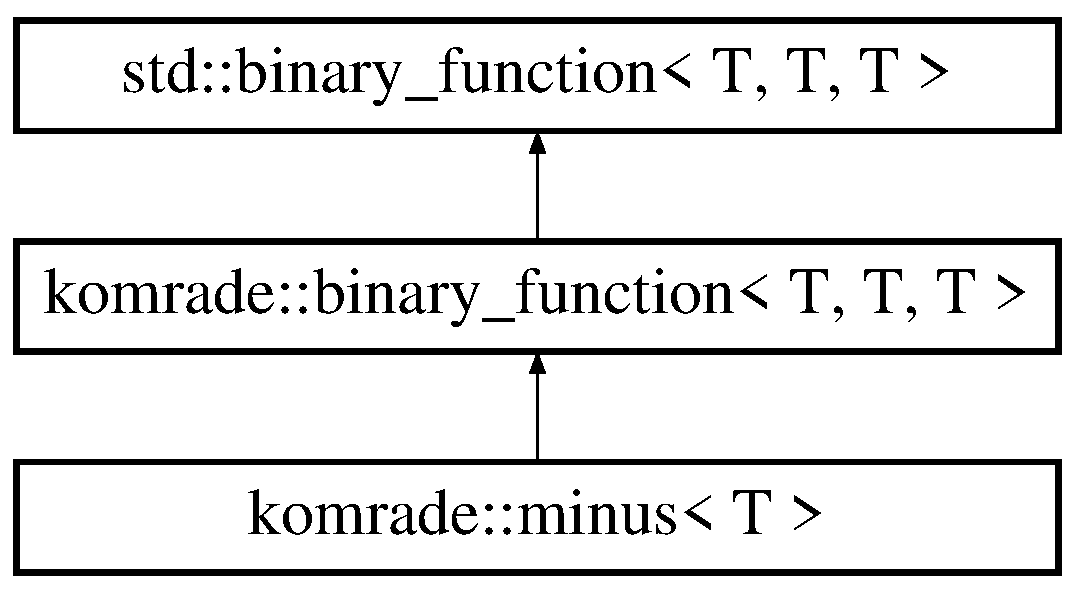
\includegraphics[height=3cm]{structkomrade_1_1minus}
\end{center}
\end{figure}
\subsection*{Public Member Functions}
\begin{CompactItemize}
\item 
\_\-\_\-host\_\-\_\- \_\-\_\-device\_\-\_\- T {\bf operator()} (const T \&lhs, const T \&rhs) const 
\end{CompactItemize}


\subsection{Detailed Description}
\subsubsection*{template$<$typename T$>$ struct komrade::minus$<$ T $>$}

{\tt \doxyref{minus}{p.}{structkomrade_1_1minus}} is a function object. Specifically, it is an Adaptable Binary Function. If {\tt f} is an object of class {\tt minus$<$T$>$}, and {\tt x} and {\tt y} are objects of class {\tt T}, then {\tt f(x,y)} returns {\tt x-y}.

\begin{Desc}
\item[Template Parameters:]
\begin{description}
\item[{\em T}]is a model of {\tt Assignable}, and if {\tt x} and {\tt y} are objects of type {\tt T}, then {\tt x-y} must be defined and must have a return type that is convertible to {\tt T}.\end{description}
\end{Desc}
The following code snippet demonstrates how to use {\tt \doxyref{minus}{p.}{structkomrade_1_1minus}} to subtract a \doxyref{device\_\-vector}{p.}{classkomrade_1_1device__vector} of {\tt floats} from another.



\begin{Code}\begin{verbatim}  #include <komrade/device_vector.h>
  #include <komrade/functional.h>
  #include <komrade/range.h>
  #include <komrade/fill.h>
  #include <komrade/transform.h>
  ...
  const int N = 1000;
  komrade::device_vector<float> V1(N);
  komrade::device_vector<float> V2(N);
  komrade::device_vector<float> V3(N);

  komrade::range(V1.begin(), V1.end(), 1);
  komrade::fill(V2.begin(), V2.end(), 75);

  komrade::transform(V1.begin(), V1.end(), V2.begin(), V3.begin(),
                     komrade::minus<float>());
  // V3 is now {-74, -75, -76, ..., -925}
\end{verbatim}
\end{Code}



\begin{Desc}
\item[See also:]{\tt http://www.sgi.com/tech/stl/minus.html} 

\doxyref{binary\_\-function}{p.}{structkomrade_1_1binary__function} \end{Desc}


\subsection{Member Function Documentation}
\index{komrade::minus@{komrade::minus}!operator()@{operator()}}
\index{operator()@{operator()}!komrade::minus@{komrade::minus}}
\subsubsection[operator()]{\setlength{\rightskip}{0pt plus 5cm}template$<$typename T$>$ \_\-\_\-host\_\-\_\- \_\-\_\-device\_\-\_\- T {\bf komrade::minus}$<$ T $>$::operator() (const T \& {\em lhs}, \/  const T \& {\em rhs}) const\hspace{0.3cm}{\tt  [inline]}}\label{structkomrade_1_1minus_192b4b876306e2b12495e6cbf3a592d7}


Function call operator. The return value is {\tt lhs - rhs}. 

The documentation for this struct was generated from the following file:\begin{CompactItemize}
\item 
{\bf functional.h}\end{CompactItemize}

\section{komrade::modulus$<$ T $>$ Struct Template Reference}
\label{structkomrade_1_1modulus}\index{komrade::modulus@{komrade::modulus}}
{\tt \#include $<$functional.h$>$}

Inheritance diagram for komrade::modulus$<$ T $>$::\begin{figure}[H]
\begin{center}
\leavevmode
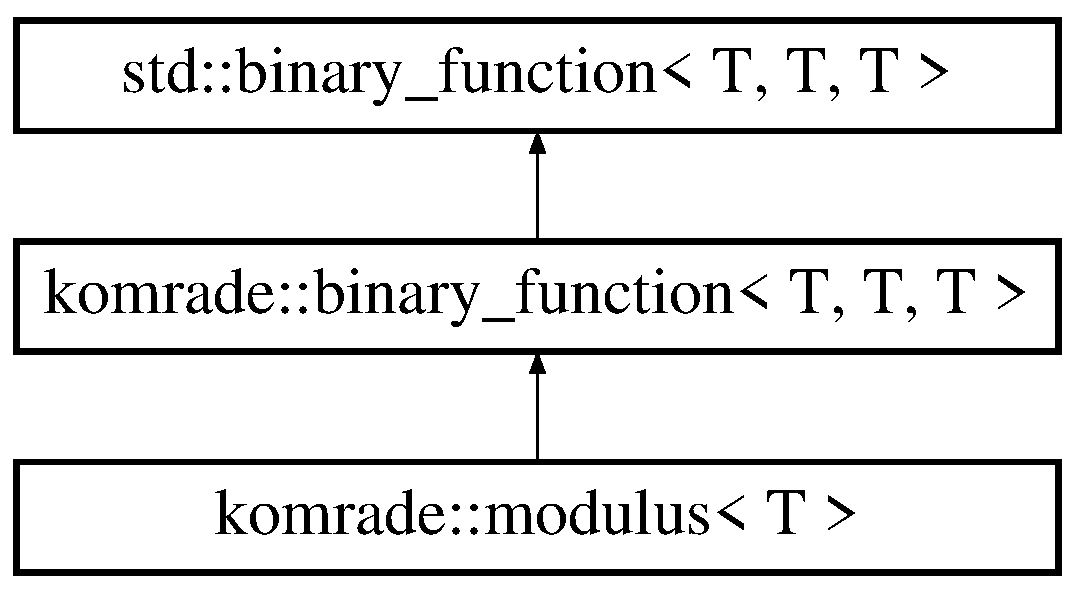
\includegraphics[height=3cm]{structkomrade_1_1modulus}
\end{center}
\end{figure}
\subsection*{Public Member Functions}
\begin{CompactItemize}
\item 
\_\-\_\-host\_\-\_\- \_\-\_\-device\_\-\_\- T {\bf operator()} (const T \&lhs, const T \&rhs) const 
\end{CompactItemize}


\subsection{Detailed Description}
\subsubsection*{template$<$typename T$>$ struct komrade::modulus$<$ T $>$}

{\tt \doxyref{modulus}{p.}{structkomrade_1_1modulus}} is a function object. Specifically, it is an Adaptable Binary Function. If {\tt f} is an object of class {\tt divides$<$T$>$}, and {\tt x} and {\tt y} are objects of class {\tt T}, then {\tt f(x,y)} returns {\tt xy}.

\begin{Desc}
\item[Template Parameters:]
\begin{description}
\item[{\em T}]is a model of {\tt Assignable}, and if {\tt x} and {\tt y} are objects of type {\tt T}, then {\tt xy} must be defined and must have a return type that is convertible to {\tt T}.\end{description}
\end{Desc}
The following code snippet demonstrates how to use {\tt \doxyref{modulus}{p.}{structkomrade_1_1modulus}} to take the \doxyref{modulus}{p.}{structkomrade_1_1modulus} of one device\_\-vectors of {\tt floats} by another.



\begin{Code}\begin{verbatim}  #include <komrade/device_vector.h>
  #include <komrade/functional.h>
  #include <komrade/range.h>
  #include <komrade/fill.h>
  #include <komrade/transform.h>
  ...
  const int N = 1000;
  komrade::device_vector<float> V1(N);
  komrade::device_vector<float> V2(N);
  komrade::device_vector<float> V3(N);

  komrade::range(V1.begin(), V1.end(), 1);
  komrade::fill(V2.begin(), V2.end(), 75);

  komrade::transform(V1.begin(), V1.end(), V2.begin(), V3.begin(),
                     komrade::modulus<int>());
  // V3 is now {1%75, 2%75, 3%75, ..., 1000%75}
\end{verbatim}
\end{Code}



\begin{Desc}
\item[See also:]{\tt http://www.sgi.com/tech/stl/modulus.html} 

\doxyref{binary\_\-function}{p.}{structkomrade_1_1binary__function} \end{Desc}


\subsection{Member Function Documentation}
\index{komrade::modulus@{komrade::modulus}!operator()@{operator()}}
\index{operator()@{operator()}!komrade::modulus@{komrade::modulus}}
\subsubsection[operator()]{\setlength{\rightskip}{0pt plus 5cm}template$<$typename T$>$ \_\-\_\-host\_\-\_\- \_\-\_\-device\_\-\_\- T {\bf komrade::modulus}$<$ T $>$::operator() (const T \& {\em lhs}, \/  const T \& {\em rhs}) const\hspace{0.3cm}{\tt  [inline]}}\label{structkomrade_1_1modulus_a0bec10e5420c838887861ef82c6f14a}


Function call operator. The return value is {\tt lhs \% rhs}. 

The documentation for this struct was generated from the following file:\begin{CompactItemize}
\item 
{\bf functional.h}\end{CompactItemize}

\section{komrade::multiplies$<$ T $>$ Struct Template Reference}
\label{structkomrade_1_1multiplies}\index{komrade::multiplies@{komrade::multiplies}}
{\tt \#include $<$functional.h$>$}

Inheritance diagram for komrade::multiplies$<$ T $>$::\begin{figure}[H]
\begin{center}
\leavevmode
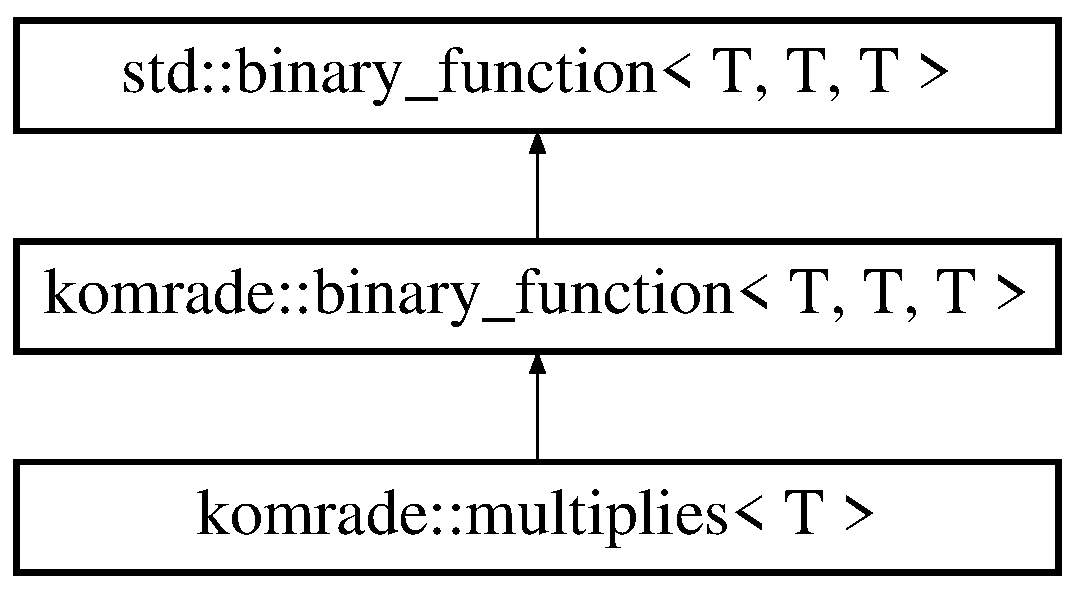
\includegraphics[height=3cm]{structkomrade_1_1multiplies}
\end{center}
\end{figure}
\subsection*{Public Member Functions}
\begin{CompactItemize}
\item 
\_\-\_\-host\_\-\_\- \_\-\_\-device\_\-\_\- T {\bf operator()} (const T \&lhs, const T \&rhs) const 
\end{CompactItemize}


\subsection{Detailed Description}
\subsubsection*{template$<$typename T$>$ struct komrade::multiplies$<$ T $>$}

{\tt \doxyref{multiplies}{p.}{structkomrade_1_1multiplies}} is a function object. Specifically, it is an Adaptable Binary Function. If {\tt f} is an object of class {\tt minus$<$T$>$}, and {\tt x} and {\tt y} are objects of class {\tt T}, then {\tt f(x,y)} returns {\tt x$\ast$y}.

\begin{Desc}
\item[Template Parameters:]
\begin{description}
\item[{\em T}]is a model of {\tt Assignable}, and if {\tt x} and {\tt y} are objects of type {\tt T}, then {\tt x$\ast$y} must be defined and must have a return type that is convertible to {\tt T}.\end{description}
\end{Desc}
The following code snippet demonstrates how to use {\tt \doxyref{multiplies}{p.}{structkomrade_1_1multiplies}} to multiply two device\_\-vectors of {\tt floats}.



\begin{Code}\begin{verbatim}  #include <komrade/device_vector.h>
  #include <komrade/functional.h>
  #include <komrade/range.h>
  #include <komrade/fill.h>
  #include <komrade/transform.h>
  ...
  const int N = 1000;
  komrade::device_vector<float> V1(N);
  komrade::device_vector<float> V2(N);
  komrade::device_vector<float> V3(N);

  komrade::range(V1.begin(), V1.end(), 1);
  komrade::fill(V2.begin(), V2.end(), 75);

  komrade::transform(V1.begin(), V1.end(), V2.begin(), V3.begin(),
                     komrade::multiplies<float>());
  // V3 is now {75, 150, 225, ..., 75000}
\end{verbatim}
\end{Code}



\begin{Desc}
\item[See also:]{\tt http://www.sgi.com/tech/stl/multiplies.html} 

\doxyref{binary\_\-function}{p.}{structkomrade_1_1binary__function} \end{Desc}


\subsection{Member Function Documentation}
\index{komrade::multiplies@{komrade::multiplies}!operator()@{operator()}}
\index{operator()@{operator()}!komrade::multiplies@{komrade::multiplies}}
\subsubsection[operator()]{\setlength{\rightskip}{0pt plus 5cm}template$<$typename T$>$ \_\-\_\-host\_\-\_\- \_\-\_\-device\_\-\_\- T {\bf komrade::multiplies}$<$ T $>$::operator() (const T \& {\em lhs}, \/  const T \& {\em rhs}) const\hspace{0.3cm}{\tt  [inline]}}\label{structkomrade_1_1multiplies_1bf149d692ddde334cc2a5d522b04cfe}


Function call operator. The return value is {\tt lhs $\ast$ rhs}. 

The documentation for this struct was generated from the following file:\begin{CompactItemize}
\item 
{\bf functional.h}\end{CompactItemize}

\section{komrade::negate$<$ T $>$ Struct Template Reference}
\label{structkomrade_1_1negate}\index{komrade::negate@{komrade::negate}}
{\tt \#include $<$functional.h$>$}

Inheritance diagram for komrade::negate$<$ T $>$::\begin{figure}[H]
\begin{center}
\leavevmode
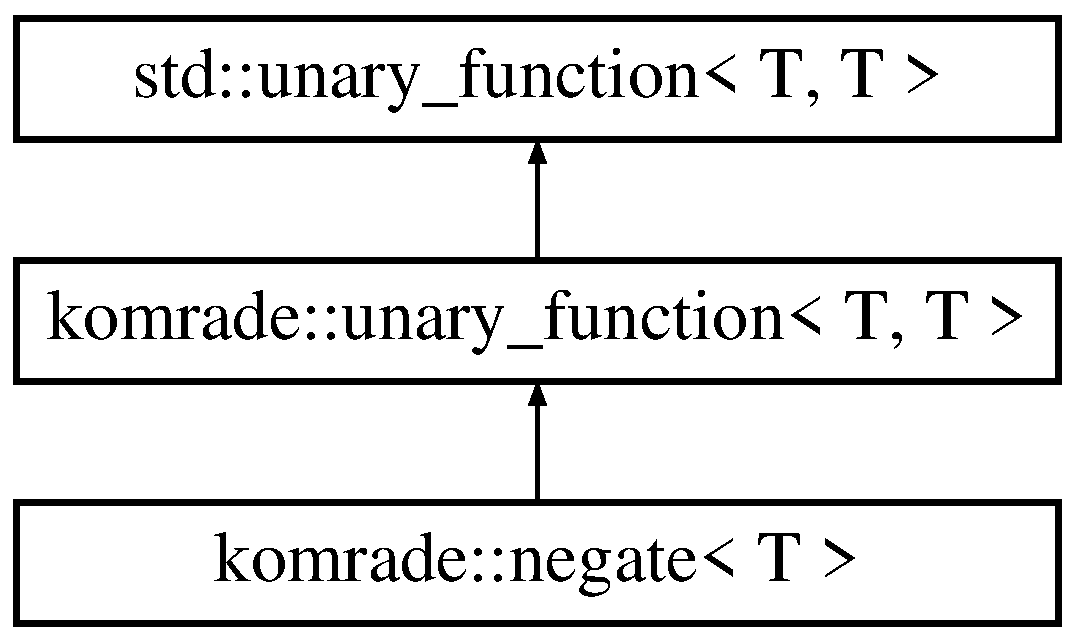
\includegraphics[height=3cm]{structkomrade_1_1negate}
\end{center}
\end{figure}
\subsection*{Public Member Functions}
\begin{CompactItemize}
\item 
\_\-\_\-host\_\-\_\- \_\-\_\-device\_\-\_\- T {\bf operator()} (const T \&x) const 
\end{CompactItemize}


\subsection{Detailed Description}
\subsubsection*{template$<$typename T$>$ struct komrade::negate$<$ T $>$}

{\tt \doxyref{negate}{p.}{structkomrade_1_1negate}} is a function object. Specifically, it is an Adaptable Unary Function. If {\tt f} is an object of class {\tt negate$<$T$>$}, and {\tt x} is an object of class {\tt T}, then {\tt f(x,y)} returns {\tt -x}.

\begin{Desc}
\item[Template Parameters:]
\begin{description}
\item[{\em T}]is a model of {\tt Assignable}, and if {\tt x} is an object of type {\tt T}, then {\tt -x} must be defined and must have a return type that is convertible to {\tt T}.\end{description}
\end{Desc}
The following code snippet demonstrates how to use {\tt \doxyref{negate}{p.}{structkomrade_1_1negate}} to \doxyref{negate}{p.}{structkomrade_1_1negate} the element of a \doxyref{device\_\-vector}{p.}{classkomrade_1_1device__vector} of {\tt floats}.



\begin{Code}\begin{verbatim}  #include <komrade/device_vector.h>
  #include <komrade/functional.h>
  #include <komrade/range.h>
  #include <komrade/transform.h>
  ...
  const int N = 1000;
  komrade::device_vector<float> V1(N);
  komrade::device_vector<float> V2(N);

  komrade::range(V1.begin(), V1.end(), 1);

  komrade::transform(V1.begin(), V1.end(), V2.begin(),
                     komrade::negate<float>());
  // V2 is now {-1, -2, -3, ..., -1000}
\end{verbatim}
\end{Code}



\begin{Desc}
\item[See also:]{\tt http://www.sgi.com/tech/stl/negate.html} 

\doxyref{unary\_\-function}{p.}{structkomrade_1_1unary__function} \end{Desc}


\subsection{Member Function Documentation}
\index{komrade::negate@{komrade::negate}!operator()@{operator()}}
\index{operator()@{operator()}!komrade::negate@{komrade::negate}}
\subsubsection[operator()]{\setlength{\rightskip}{0pt plus 5cm}template$<$typename T$>$ \_\-\_\-host\_\-\_\- \_\-\_\-device\_\-\_\- T {\bf komrade::negate}$<$ T $>$::operator() (const T \& {\em x}) const\hspace{0.3cm}{\tt  [inline]}}\label{structkomrade_1_1negate_51011f23a38c93abec8bd66aaa70e9cf}


Function call operator. The return value is {\tt -x}. 

The documentation for this struct was generated from the following file:\begin{CompactItemize}
\item 
{\bf functional.h}\end{CompactItemize}

\section{komrade::not\_\-equal\_\-to$<$ T $>$ Struct Template Reference}
\label{structkomrade_1_1not__equal__to}\index{komrade::not\_\-equal\_\-to@{komrade::not\_\-equal\_\-to}}
{\tt \#include $<$functional.h$>$}

Inheritance diagram for komrade::not\_\-equal\_\-to$<$ T $>$::\begin{figure}[H]
\begin{center}
\leavevmode
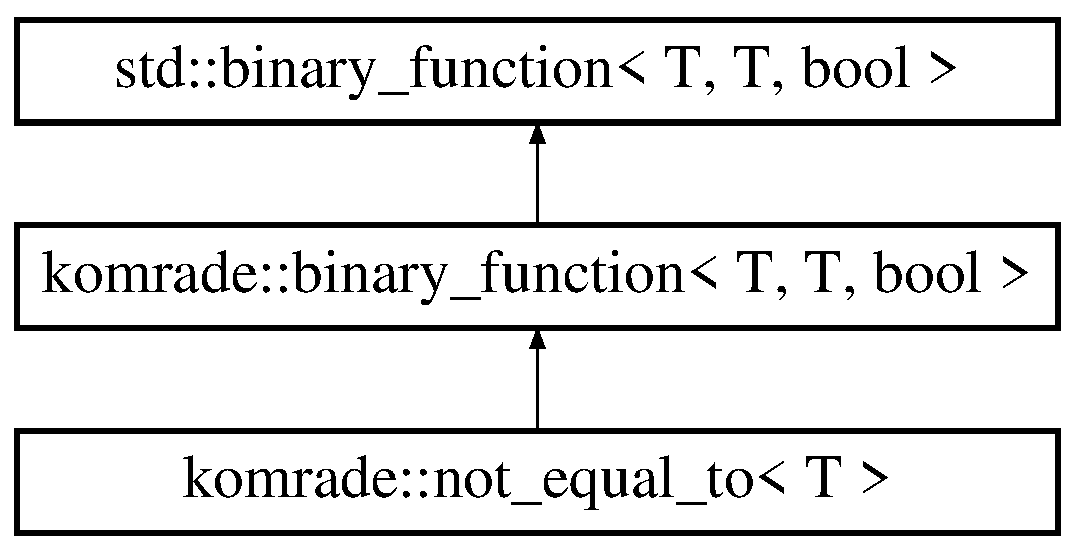
\includegraphics[height=3cm]{structkomrade_1_1not__equal__to}
\end{center}
\end{figure}
\subsection*{Public Member Functions}
\begin{CompactItemize}
\item 
\_\-\_\-host\_\-\_\- \_\-\_\-device\_\-\_\- bool {\bf operator()} (const T \&lhs, const T \&rhs) const 
\end{CompactItemize}


\subsection{Detailed Description}
\subsubsection*{template$<$typename T$>$ struct komrade::not\_\-equal\_\-to$<$ T $>$}

{\tt \doxyref{not\_\-equal\_\-to}{p.}{structkomrade_1_1not__equal__to}} is a function object. Specifically, it is an Adaptable Binary Predicate, which means it is a function object that tests the truth or falsehood of some condition. If {\tt f} is an object of class {\tt not\_\-equal\_\-to$<$T$>$} and {\tt x} and {\tt y} are objects of class {\tt T}, then {\tt f(x,y)} returns {\tt true} if {\tt x != y} and {\tt false} otherwise.

\begin{Desc}
\item[Template Parameters:]
\begin{description}
\item[{\em T}]is a model of {\tt Equality Comparable}.\end{description}
\end{Desc}
\begin{Desc}
\item[See also:]{\tt http://www.sgi.com/tech/stl/not\_\-equal\_\-to.html} 

\doxyref{binary\_\-function}{p.}{structkomrade_1_1binary__function} \end{Desc}


\subsection{Member Function Documentation}
\index{komrade::not\_\-equal\_\-to@{komrade::not\_\-equal\_\-to}!operator()@{operator()}}
\index{operator()@{operator()}!komrade::not_equal_to@{komrade::not\_\-equal\_\-to}}
\subsubsection[operator()]{\setlength{\rightskip}{0pt plus 5cm}template$<$typename T$>$ \_\-\_\-host\_\-\_\- \_\-\_\-device\_\-\_\- bool {\bf komrade::not\_\-equal\_\-to}$<$ T $>$::operator() (const T \& {\em lhs}, \/  const T \& {\em rhs}) const\hspace{0.3cm}{\tt  [inline]}}\label{structkomrade_1_1not__equal__to_c40e22e5c692d8533dbc137754d0549f}


Function call operator. The return value is {\tt lhs != rhs}. 

The documentation for this struct was generated from the following file:\begin{CompactItemize}
\item 
{\bf functional.h}\end{CompactItemize}

\section{komrade::output\_\-device\_\-iterator\_\-tag Struct Reference}
\label{structkomrade_1_1output__device__iterator__tag}\index{komrade::output\_\-device\_\-iterator\_\-tag@{komrade::output\_\-device\_\-iterator\_\-tag}}
{\tt \#include $<$iterator\_\-categories.h$>$}



\subsection{Detailed Description}
{\tt \doxyref{output\_\-device\_\-iterator\_\-tag}{p.}{structkomrade_1_1output__device__iterator__tag}} is an empty class: it has no member functions, member variables, or nested types. It is used solely as a \char`\"{}tag\char`\"{}: a representation of the Output Device Iterator concept within the C++ type system.

\begin{Desc}
\item[See also:]{\tt http://www.sgi.com/tech/sgi/output\_\-iterator\_\-tag.html,} iterator\_\-traits, \doxyref{input\_\-device\_\-iterator\_\-tag}{p.}{structkomrade_1_1input__device__iterator__tag}, \doxyref{forward\_\-device\_\-iterator\_\-tag}{p.}{structkomrade_1_1forward__device__iterator__tag}, \doxyref{bidirectional\_\-device\_\-iterator\_\-tag}{p.}{structkomrade_1_1bidirectional__device__iterator__tag}, \doxyref{random\_\-access\_\-device\_\-iterator\_\-tag}{p.}{structkomrade_1_1random__access__device__iterator__tag}, \doxyref{input\_\-host\_\-iterator\_\-tag}{p.}{group__iterator__tag__classes_g0927e3a6aecf64b535bd28052c7516d5}, \doxyref{output\_\-host\_\-iterator\_\-tag}{p.}{group__iterator__tag__classes_gba20a59557406e3ab657831abf6d65a0}, \doxyref{forward\_\-host\_\-iterator\_\-tag}{p.}{group__iterator__tag__classes_gc0af280b47824bd61134805db6ffe828}, \doxyref{bidirectional\_\-host\_\-iterator\_\-tag}{p.}{group__iterator__tag__classes_gbdabd9cb52934a67a931cfd93d6079f0}, \doxyref{random\_\-access\_\-host\_\-iterator\_\-tag}{p.}{group__iterator__tag__classes_gfde808d31f9339adeda3dcf88077da8d} \end{Desc}


The documentation for this struct was generated from the following file:\begin{CompactItemize}
\item 
{\bf iterator\_\-categories.h}\end{CompactItemize}

\section{komrade::plus$<$ T $>$ Struct Template Reference}
\label{structkomrade_1_1plus}\index{komrade::plus@{komrade::plus}}
{\tt \#include $<$functional.h$>$}

Inheritance diagram for komrade::plus$<$ T $>$::\begin{figure}[H]
\begin{center}
\leavevmode
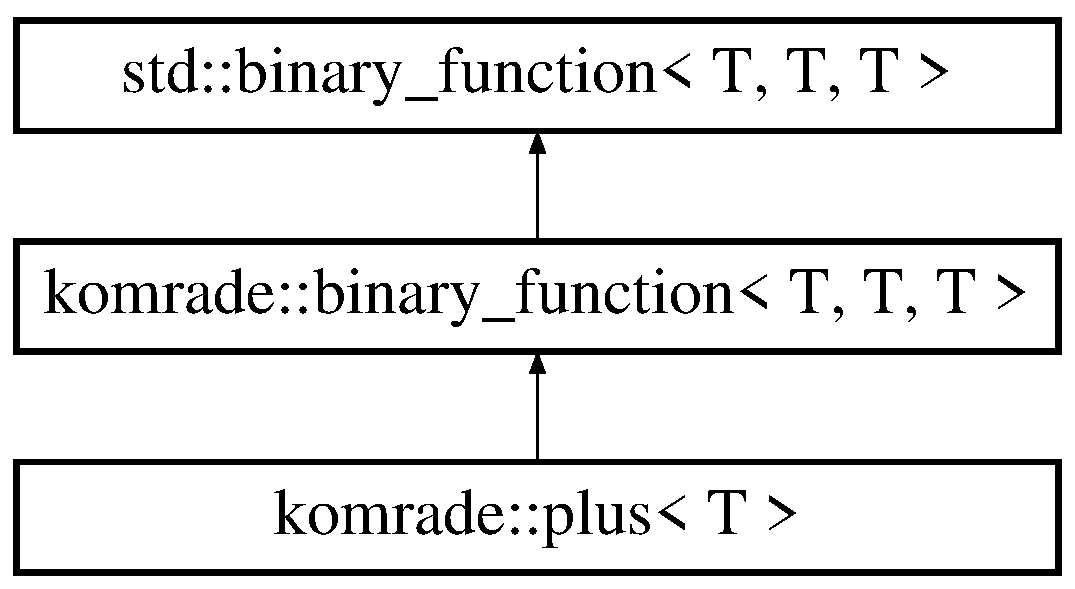
\includegraphics[height=3cm]{structkomrade_1_1plus}
\end{center}
\end{figure}
\subsection*{Public Member Functions}
\begin{CompactItemize}
\item 
\_\-\_\-host\_\-\_\- \_\-\_\-device\_\-\_\- T {\bf operator()} (const T \&lhs, const T \&rhs) const 
\end{CompactItemize}


\subsection{Detailed Description}
\subsubsection*{template$<$typename T$>$ struct komrade::plus$<$ T $>$}

{\tt \doxyref{plus}{p.}{structkomrade_1_1plus}} is a function object. Specifically, it is an Adaptable Binary Function. If {\tt f} is an object of class {\tt plus$<$T$>$}, and {\tt x} and {\tt y} are objects of class {\tt T}, then {\tt f(x,y)} returns {\tt x+y}.

\begin{Desc}
\item[Template Parameters:]
\begin{description}
\item[{\em T}]is a model of {\tt Assignable}, and if {\tt x} and {\tt y} are objects of type {\tt T}, then {\tt x+y} must be defined and must have a return type that is convertible to {\tt T}.\end{description}
\end{Desc}
The following code snippet demonstrates how to use {\tt \doxyref{plus}{p.}{structkomrade_1_1plus}} to sum two device\_\-vectors of {\tt floats}.



\begin{Code}\begin{verbatim}  #include <komrade/device_vector.h>
  #include <komrade/functional.h>
  #include <komrade/range.h>
  #include <komrade/fill.h>
  #include <komrade/transform.h>
  ...
  const int N = 1000;
  komrade::device_vector<float> V1(N);
  komrade::device_vector<float> V2(N);
  komrade::device_vector<float> V3(N);

  komrade::range(V1.begin(), V1.end(), 1);
  komrade::fill(V2.begin(), V2.end(), 75);

  komrade::transform(V1.begin(), V1.end(), V2.begin(), V3.begin(),
                     komrade::plus<float>());
  // V3 is now {76, 77, 78, ..., 1075}
\end{verbatim}
\end{Code}



\begin{Desc}
\item[See also:]{\tt http://www.sgi.com/tech/stl/plus.html} 

\doxyref{binary\_\-function}{p.}{structkomrade_1_1binary__function} \end{Desc}


\subsection{Member Function Documentation}
\index{komrade::plus@{komrade::plus}!operator()@{operator()}}
\index{operator()@{operator()}!komrade::plus@{komrade::plus}}
\subsubsection[operator()]{\setlength{\rightskip}{0pt plus 5cm}template$<$typename T$>$ \_\-\_\-host\_\-\_\- \_\-\_\-device\_\-\_\- T {\bf komrade::plus}$<$ T $>$::operator() (const T \& {\em lhs}, \/  const T \& {\em rhs}) const\hspace{0.3cm}{\tt  [inline]}}\label{structkomrade_1_1plus_b647a0f91120ceefb8dd7edd1fdf1a6c}


Function call operator. The return value is {\tt lhs + rhs}. 

The documentation for this struct was generated from the following file:\begin{CompactItemize}
\item 
{\bf functional.h}\end{CompactItemize}

\section{komrade::random\_\-access\_\-device\_\-iterator\_\-tag Struct Reference}
\label{structkomrade_1_1random__access__device__iterator__tag}\index{komrade::random\_\-access\_\-device\_\-iterator\_\-tag@{komrade::random\_\-access\_\-device\_\-iterator\_\-tag}}
{\tt \#include $<$iterator\_\-categories.h$>$}

Inheritance diagram for komrade::random\_\-access\_\-device\_\-iterator\_\-tag::\begin{figure}[H]
\begin{center}
\leavevmode
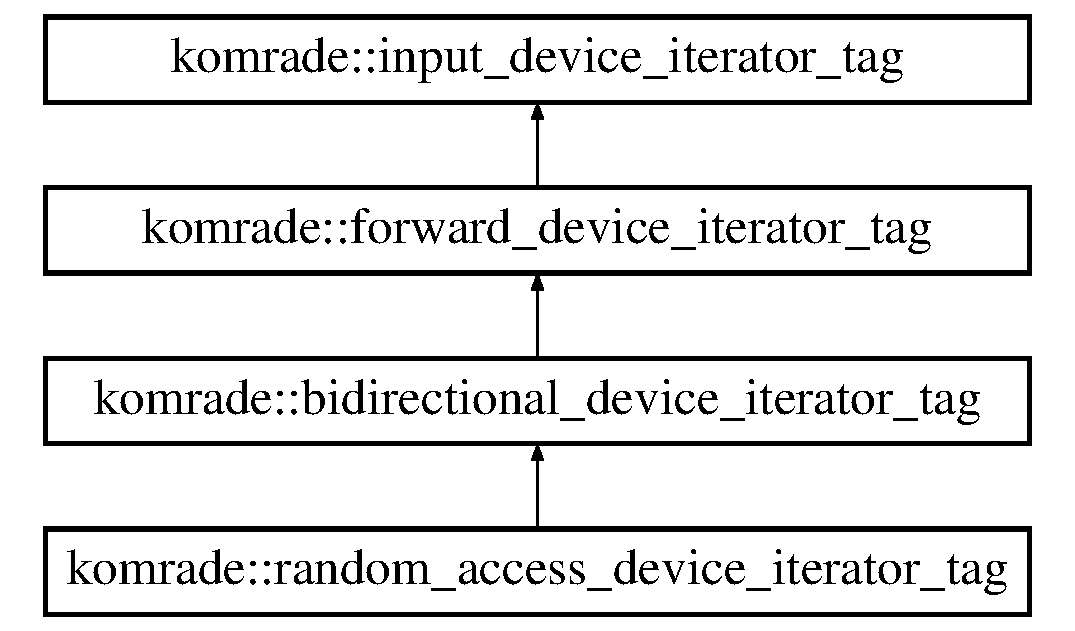
\includegraphics[height=4cm]{structkomrade_1_1random__access__device__iterator__tag}
\end{center}
\end{figure}


\subsection{Detailed Description}
{\tt \doxyref{random\_\-access\_\-device\_\-iterator\_\-tag}{p.}{structkomrade_1_1random__access__device__iterator__tag}} is an empty class: it has no member functions, member variables, or nested types. It is used solely as a \char`\"{}tag\char`\"{}: a representation of the Random Access Device Iterator concept within the C++ type system.

\begin{Desc}
\item[See also:]{\tt http://www.sgi.com/tech/sgi/random\_\-access\_\-iterator\_\-tag.html,} iterator\_\-traits, \doxyref{input\_\-device\_\-iterator\_\-tag}{p.}{structkomrade_1_1input__device__iterator__tag}, \doxyref{output\_\-device\_\-iterator\_\-tag}{p.}{structkomrade_1_1output__device__iterator__tag}, \doxyref{forward\_\-device\_\-iterator\_\-tag}{p.}{structkomrade_1_1forward__device__iterator__tag}, \doxyref{bidirectional\_\-device\_\-iterator\_\-tag}{p.}{structkomrade_1_1bidirectional__device__iterator__tag}, \doxyref{input\_\-host\_\-iterator\_\-tag}{p.}{group__iterator__tag__classes_g0927e3a6aecf64b535bd28052c7516d5}, \doxyref{output\_\-host\_\-iterator\_\-tag}{p.}{group__iterator__tag__classes_gba20a59557406e3ab657831abf6d65a0}, \doxyref{forward\_\-host\_\-iterator\_\-tag}{p.}{group__iterator__tag__classes_gc0af280b47824bd61134805db6ffe828}, \doxyref{bidirectional\_\-host\_\-iterator\_\-tag}{p.}{group__iterator__tag__classes_gbdabd9cb52934a67a931cfd93d6079f0}, \doxyref{random\_\-access\_\-host\_\-iterator\_\-tag}{p.}{group__iterator__tag__classes_gfde808d31f9339adeda3dcf88077da8d} \end{Desc}


The documentation for this struct was generated from the following file:\begin{CompactItemize}
\item 
{\bf iterator\_\-categories.h}\end{CompactItemize}

\section{komrade::unary\_\-function$<$ Argument, Result $>$ Struct Template Reference}
\label{structkomrade_1_1unary__function}\index{komrade::unary\_\-function@{komrade::unary\_\-function}}
{\tt \#include $<$functional.h$>$}



\subsection{Detailed Description}
\subsubsection*{template$<$typename Argument, typename Result$>$ struct komrade::unary\_\-function$<$ Argument, Result $>$}

{\tt \doxyref{unary\_\-function}{p.}{structkomrade_1_1unary__function}} is an empty base class: it contains no member functions or member variables, but only type information. The only reason it exists is to make it more convenient to define types that are models of the concept Adaptable Unary Function. Specifically, any model of Adaptable Unary Function must define nested {\tt typedefs}. Those {\tt typedefs} are provided by the base class {\tt \doxyref{unary\_\-function}{p.}{structkomrade_1_1unary__function}}.

The following code snippet demonstrates how to construct an Adaptable Unary Function using {\tt \doxyref{unary\_\-function}{p.}{structkomrade_1_1unary__function}}.



\begin{Code}\begin{verbatim}  struct sine : public komrade::unary_function<float,float>
  {
    __host__ __device__
    double operator()(float x) { return sinf(x); }
  };
\end{verbatim}
\end{Code}



\begin{Desc}
\item[Note:]\doxyref{unary\_\-function}{p.}{structkomrade_1_1unary__function} is currently redundant with the C++ STL type {\tt std::unary\_\-function}. We reserve it here for potential additional functionality at a later date.\end{Desc}
\begin{Desc}
\item[See also:]{\tt http://www.sgi.com/tech/stl/unary\_\-function.html} 

\doxyref{binary\_\-function}{p.}{structkomrade_1_1binary__function} \end{Desc}


The documentation for this struct was generated from the following file:\begin{CompactItemize}
\item 
{\bf functional.h}\end{CompactItemize}

\section{komrade::unary\_\-negate$<$ Predicate $>$ Struct Template Reference}
\label{structkomrade_1_1unary__negate}\index{komrade::unary\_\-negate@{komrade::unary\_\-negate}}
{\tt \#include $<$functional.h$>$}

\subsection*{Public Member Functions}
\begin{CompactItemize}
\item 
\_\-\_\-host\_\-\_\- \_\-\_\-device\_\-\_\- \textbf{unary\_\-negate} (Predicate p)\label{structkomrade_1_1unary__negate_0c0832148ad458d9e7fead7fa00d1442}

\item 
{\footnotesize template$<$typename T$>$ }\\\_\-\_\-host\_\-\_\- \_\-\_\-device\_\-\_\- bool {\bf operator()} (const T x)
\end{CompactItemize}
\subsection*{Public Attributes}
\begin{CompactItemize}
\item 
Predicate \textbf{pred}\label{structkomrade_1_1unary__negate_fe73a049350f9bf9894887aec7d266a0}

\end{CompactItemize}


\subsection{Detailed Description}
\subsubsection*{template$<$typename Predicate$>$ struct komrade::unary\_\-negate$<$ Predicate $>$}

{\tt \doxyref{unary\_\-negate}{p.}{structkomrade_1_1unary__negate}} is a function object adaptor: it is an Adaptable Predicate that represents the logical negation of some other Adaptable Predicate. That is: if {\tt f} is an object of class {\tt unary\_\-negate$<$AdaptablePredicate$>$}, then there exists an object {\tt pred} of class {\tt AdaptablePredicate} such that {\tt f(x)} always returns the same value as {\tt !pred(x)}. There is rarely any reason to construct a {\tt \doxyref{unary\_\-negate}{p.}{structkomrade_1_1unary__negate}} directly; it is almost always easier to use the helper function not1.

\begin{Desc}
\item[See also:]{\tt http://www.sgi.com/tech/stl/unary\_\-negate.html} 

\doxyref{not1}{p.}{group__function__object__adaptors_ga3fbfed5c41580041c606815acabd5bb} \end{Desc}


\subsection{Member Function Documentation}
\index{komrade::unary\_\-negate@{komrade::unary\_\-negate}!operator()@{operator()}}
\index{operator()@{operator()}!komrade::unary_negate@{komrade::unary\_\-negate}}
\subsubsection[operator()]{\setlength{\rightskip}{0pt plus 5cm}template$<$typename Predicate$>$ template$<$typename T$>$ \_\-\_\-host\_\-\_\- \_\-\_\-device\_\-\_\- bool {\bf komrade::unary\_\-negate}$<$ Predicate $>$::operator() (const T {\em x})\hspace{0.3cm}{\tt  [inline]}}\label{structkomrade_1_1unary__negate_9c2474a78f4822ece812c7dc42456ae6}


Function call operator. The return value is {\tt !pred(x)}. 

The documentation for this struct was generated from the following file:\begin{CompactItemize}
\item 
{\bf functional.h}\end{CompactItemize}

\chapter{File Documentation}
\section{adjacent\_\-difference.h File Reference}
\label{adjacent__difference_8h}\index{adjacent\_\-difference.h@{adjacent\_\-difference.h}}
Compute difference between consecutive elements of a sequence. 

{\tt \#include $<$komrade/detail/config.h$>$}\par
{\tt \#include $<$komrade/detail/adjacent\_\-difference.inl$>$}\par
\subsection*{Namespaces}
\begin{CompactItemize}
\item 
namespace {\bf komrade}
\end{CompactItemize}
\subsection*{Functions}
\begin{CompactItemize}
\item 
{\footnotesize template$<$typename InputIterator, typename OutputIterator$>$ }\\OutputIterator {\bf komrade::adjacent\_\-difference} (InputIterator first, InputIterator last, OutputIterator result)
\item 
{\footnotesize template$<$typename InputIterator, typename OutputIterator, typename BinaryFunction$>$ }\\OutputIterator {\bf komrade::adjacent\_\-difference} (InputIterator first, InputIterator last, OutputIterator result, BinaryFunction binary\_\-op)
\end{CompactItemize}


\subsection{Detailed Description}
Compute difference between consecutive elements of a sequence. 


\section{arch.h File Reference}
\label{arch_8h}\index{arch.h@{arch.h}}
Defines the interface to functions providing introspection into the architecture of CUDA devices. 

{\tt \#include $<$komrade/detail/config.h$>$}\par
{\tt \#include $<$cstddef$>$}\par
{\tt \#include $<$vector\_\-types.h$>$}\par
{\tt \#include $<$komrade/experimental/arch.inl$>$}\par
\subsection*{Namespaces}
\begin{CompactItemize}
\item 
namespace {\bf komrade}
\item 
namespace {\bf komrade::experimental}
\item 
namespace \textbf{komrade::experimental::arch}
\end{CompactItemize}
\subsection*{Functions}
\begin{CompactItemize}
\item 
size\_\-t {\bf komrade::experimental::arch::num\_\-multiprocessors} (void)
\item 
size\_\-t {\bf komrade::experimental::arch::max\_\-active\_\-threads\_\-per\_\-multiprocessor} (void)
\item 
size\_\-t {\bf komrade::experimental::arch::max\_\-active\_\-threads} (void)
\item 
dim3 {\bf komrade::experimental::arch::max\_\-grid\_\-dimensions} (void)
\end{CompactItemize}


\subsection{Detailed Description}
Defines the interface to functions providing introspection into the architecture of CUDA devices. 


\section{arch.inl File Reference}
\label{arch_8inl}\index{arch.inl@{arch.inl}}
Inline file for \doxyref{arch.h}{p.}{arch_8h}. 

{\tt \#include $<$assert.h$>$}\par
{\tt \#include $<$stdio.h$>$}\par
{\tt \#include $<$komrade/experimental/arch.h$>$}\par
{\tt \#include $<$vector\_\-functions.h$>$}\par
\subsection*{Namespaces}
\begin{CompactItemize}
\item 
namespace {\bf komrade}
\item 
namespace {\bf komrade::experimental}
\item 
namespace \textbf{komrade::experimental::arch}
\end{CompactItemize}
\subsection*{Functions}
\begin{CompactItemize}
\item 
size\_\-t {\bf komrade::experimental::arch::num\_\-multiprocessors} (void)
\item 
size\_\-t {\bf komrade::experimental::arch::max\_\-active\_\-threads\_\-per\_\-multiprocessor} (void)
\item 
size\_\-t {\bf komrade::experimental::arch::max\_\-active\_\-threads} (void)
\item 
dim3 {\bf komrade::experimental::arch::max\_\-grid\_\-dimensions} (void)
\end{CompactItemize}


\subsection{Detailed Description}
Inline file for \doxyref{arch.h}{p.}{arch_8h}. 


\section{constant\_\-iterator.h File Reference}
\label{constant__iterator_8h}\index{constant\_\-iterator.h@{constant\_\-iterator.h}}
Defines the interface to an iterator which returns a constant value when dereferenced. 

{\tt \#include $<$komrade/detail/config.h$>$}\par
{\tt \#include $<$komrade/iterator/iterator\_\-adaptor.h$>$}\par
{\tt \#include $<$komrade/iterator/counting\_\-iterator.h$>$}\par
{\tt \#include $<$komrade/iterator/iterator\_\-categories.h$>$}\par
\subsection*{Namespaces}
\begin{CompactItemize}
\item 
namespace {\bf komrade}
\item 
namespace {\bf komrade::experimental}
\item 
namespace \textbf{komrade::detail}
\end{CompactItemize}
\subsection*{Classes}
\begin{CompactItemize}
\item 
class \textbf{komrade::experimental::constant\_\-iterator$<$ Value $>$}
\item 
struct \textbf{komrade::detail::make\_\-device\_\-dereferenceable$<$ komrade::experimental::constant\_\-iterator$<$ T $>$ $>$}
\end{CompactItemize}
\subsection*{Functions}
\begin{CompactItemize}
\item 
{\footnotesize template$<$typename T$>$ }\\\_\-\_\-host\_\-\_\- \_\-\_\-device\_\-\_\- constant\_\-iterator$<$ T $>$ \textbf{komrade::experimental::make\_\-constant\_\-iterator} (T x, ptrdiff\_\-t c=ptrdiff\_\-t())\label{namespacekomrade_1_1experimental_ee459d0d41235d9c3cf69258fc873d57}

\end{CompactItemize}


\subsection{Detailed Description}
Defines the interface to an iterator which returns a constant value when dereferenced. 


\section{copy.h File Reference}
\label{copy_8h}\index{copy.h@{copy.h}}
Defines the interface to copy between containers. 

{\tt \#include $<$komrade/detail/config.h$>$}\par
{\tt \#include $<$komrade/detail/copy.inl$>$}\par
\subsection*{Namespaces}
\begin{CompactItemize}
\item 
namespace {\bf komrade}
\end{CompactItemize}
\subsection*{Functions}
\begin{CompactItemize}
\item 
{\footnotesize template$<$typename InputIterator, typename OutputIterator$>$ }\\OutputIterator {\bf komrade::copy} (InputIterator first, InputIterator last, OutputIterator result)
\item 
{\footnotesize template$<$typename InputIterator, typename PredicateIterator, typename OutputIterator$>$ }\\OutputIterator {\bf komrade::copy\_\-if} (InputIterator first, InputIterator last, PredicateIterator stencil, OutputIterator result)
\item 
{\footnotesize template$<$typename InputIterator, typename PredicateIterator, typename OutputIterator, typename Predicate$>$ }\\OutputIterator {\bf komrade::copy\_\-if} (InputIterator begin, InputIterator end, PredicateIterator stencil, OutputIterator result, Predicate pred)
\end{CompactItemize}


\subsection{Detailed Description}
Defines the interface to copy between containers. 


\section{count.h File Reference}
\label{count_8h}\index{count.h@{count.h}}
Defines the interface to templated count and count\_\-if functions. 

{\tt \#include $<$komrade/detail/config.h$>$}\par
{\tt \#include $<$komrade/iterator/iterator\_\-traits.h$>$}\par
{\tt \#include $<$komrade/detail/count.inl$>$}\par
\subsection*{Namespaces}
\begin{CompactItemize}
\item 
namespace {\bf komrade}
\end{CompactItemize}
\subsection*{Functions}
\begin{CompactItemize}
\item 
{\footnotesize template$<$class InputIterator, class EqualityComparable$>$ }\\komrade::iterator\_\-traits$<$ InputIterator $>$::difference\_\-type {\bf komrade::count} (InputIterator first, InputIterator last, const EqualityComparable \&value)
\item 
{\footnotesize template$<$class InputIterator, class Predicate$>$ }\\komrade::iterator\_\-traits$<$ InputIterator $>$::difference\_\-type {\bf komrade::count\_\-if} (InputIterator first, InputIterator last, Predicate pred)
\end{CompactItemize}


\subsection{Detailed Description}
Defines the interface to templated count and count\_\-if functions. 


\section{counting\_\-iterator.h File Reference}
\label{counting__iterator_8h}\index{counting\_\-iterator.h@{counting\_\-iterator.h}}
Defines the interface to an iterator which adapts an incrementable type to return the current value of the incrementable upon operator$\ast$(). Based on Boost's counting\_\-iterator class. 

{\tt \#include $<$komrade/detail/config.h$>$}\par
{\tt \#include $<$komrade/iterator/iterator\_\-adaptor.h$>$}\par
{\tt \#include $<$komrade/iterator/iterator\_\-categories.h$>$}\par
\subsection*{Namespaces}
\begin{CompactItemize}
\item 
namespace {\bf komrade}
\item 
namespace {\bf komrade::experimental}
\item 
namespace \textbf{komrade::detail}
\end{CompactItemize}
\subsection*{Classes}
\begin{CompactItemize}
\item 
class \textbf{komrade::experimental::counting\_\-iterator$<$ Incrementable, Difference $>$}
\item 
struct \textbf{komrade::detail::make\_\-device\_\-dereferenceable$<$ komrade::experimental::counting\_\-iterator$<$ Incrementable, Difference $>$ $>$}
\end{CompactItemize}
\subsection*{Functions}
\begin{CompactItemize}
\item 
{\footnotesize template$<$typename Incrementable, typename Difference$>$ }\\counting\_\-iterator$<$ Incrementable, Difference $>$ \textbf{komrade::experimental::make\_\-counting\_\-iterator} (Incrementable x)\label{namespacekomrade_1_1experimental_6b2d1b48130fda953643ec1914b0784a}

\end{CompactItemize}


\subsection{Detailed Description}
Defines the interface to an iterator which adapts an incrementable type to return the current value of the incrementable upon operator$\ast$(). Based on Boost's counting\_\-iterator class. 


\section{device\_\-allocator.h File Reference}
\label{device__allocator_8h}\index{device\_\-allocator.h@{device\_\-allocator.h}}
Defines the interface to a standard C++ allocator class for allocating device memory. 

{\tt \#include $<$komrade/detail/config.h$>$}\par
{\tt \#include $<$komrade/device\_\-new\_\-allocator.h$>$}\par
{\tt \#include $<$limits$>$}\par
{\tt \#include $<$stdexcept$>$}\par
\subsection*{Namespaces}
\begin{CompactItemize}
\item 
namespace {\bf komrade}
\end{CompactItemize}
\subsection*{Classes}
\begin{CompactItemize}
\item 
class {\bf komrade::device\_\-allocator$<$ void $>$}
\item 
struct \textbf{komrade::device\_\-allocator$<$ void $>$::rebind$<$ U $>$}
\item 
class {\bf komrade::device\_\-allocator$<$ T $>$}
\item 
struct \textbf{komrade::device\_\-allocator$<$ T $>$::rebind$<$ U $>$}
\end{CompactItemize}


\subsection{Detailed Description}
Defines the interface to a standard C++ allocator class for allocating device memory. 


\section{device\_\-delete.h File Reference}
\label{device__delete_8h}\index{device\_\-delete.h@{device\_\-delete.h}}
Defines the interface to a wrapper for cudaFree. 

{\tt \#include $<$komrade/detail/config.h$>$}\par
{\tt \#include $<$komrade/device\_\-ptr.h$>$}\par
{\tt \#include $<$komrade/detail/device\_\-delete.inl$>$}\par
\subsection*{Namespaces}
\begin{CompactItemize}
\item 
namespace {\bf komrade}
\end{CompactItemize}
\subsection*{Functions}
\begin{CompactItemize}
\item 
{\footnotesize template$<$typename T$>$ }\\void {\bf komrade::device\_\-delete} ({\bf komrade::device\_\-ptr}$<$ T $>$ ptr)
\end{CompactItemize}


\subsection{Detailed Description}
Defines the interface to a wrapper for cudaFree. 


\section{device\_\-free.h File Reference}
\label{device__free_8h}\index{device\_\-free.h@{device\_\-free.h}}
Defines the entry point to a function for deallocating device storage. 

{\tt \#include $<$komrade/detail/config.h$>$}\par
{\tt \#include $<$komrade/device\_\-ptr.h$>$}\par
{\tt \#include $<$komrade/detail/device\_\-free.inl$>$}\par
\subsection*{Namespaces}
\begin{CompactItemize}
\item 
namespace {\bf komrade}
\end{CompactItemize}
\subsection*{Functions}
\begin{CompactItemize}
\item 
void {\bf komrade::device\_\-free} ({\bf komrade::device\_\-ptr}$<$ void $>$ ptr)
\end{CompactItemize}


\subsection{Detailed Description}
Defines the entry point to a function for deallocating device storage. 


\section{device\_\-malloc.h File Reference}
\label{device__malloc_8h}\index{device\_\-malloc.h@{device\_\-malloc.h}}
Defines the entry point to a function for allocating device storage. 

{\tt \#include $<$komrade/detail/config.h$>$}\par
{\tt \#include $<$komrade/device\_\-ptr.h$>$}\par
{\tt \#include $<$cstddef$>$}\par
{\tt \#include $<$komrade/detail/device\_\-malloc.inl$>$}\par
\subsection*{Namespaces}
\begin{CompactItemize}
\item 
namespace {\bf komrade}
\end{CompactItemize}
\subsection*{Functions}
\begin{CompactItemize}
\item 
{\bf komrade::device\_\-ptr}$<$ void $>$ {\bf komrade::device\_\-malloc} (const std::size\_\-t n)
\end{CompactItemize}


\subsection{Detailed Description}
Defines the entry point to a function for allocating device storage. 


\section{device\_\-new.h File Reference}
\label{device__new_8h}\index{device\_\-new.h@{device\_\-new.h}}
Defines the interface for a wrapper for cudaMalloc. 

{\tt \#include $<$komrade/detail/config.h$>$}\par
{\tt \#include $<$cstddef$>$}\par
{\tt \#include $<$komrade/device\_\-ptr.h$>$}\par
{\tt \#include $<$komrade/detail/device\_\-new.inl$>$}\par
\subsection*{Namespaces}
\begin{CompactItemize}
\item 
namespace {\bf komrade}
\end{CompactItemize}
\subsection*{Functions}
\begin{CompactItemize}
\item 
{\footnotesize template$<$typename T$>$ }\\device\_\-ptr$<$ T $>$ {\bf komrade::device\_\-new} (device\_\-ptr$<$ void $>$ p, const size\_\-t n=1)
\item 
{\footnotesize template$<$typename T$>$ }\\device\_\-ptr$<$ T $>$ {\bf komrade::device\_\-new} (device\_\-ptr$<$ void $>$ p, const T \&exemplar, const size\_\-t n=1)
\item 
{\footnotesize template$<$typename T$>$ }\\device\_\-ptr$<$ T $>$ {\bf komrade::device\_\-new} (const size\_\-t n=1)
\end{CompactItemize}


\subsection{Detailed Description}
Defines the interface for a wrapper for cudaMalloc. 


\section{device\_\-new\_\-allocator.h File Reference}
\label{device__new__allocator_8h}\index{device\_\-new\_\-allocator.h@{device\_\-new\_\-allocator.h}}
Defines the interface to a standard C++ allocator class for allocating device memory with device\_\-new. 

{\tt \#include $<$komrade/detail/config.h$>$}\par
{\tt \#include $<$komrade/device\_\-ptr.h$>$}\par
{\tt \#include $<$komrade/device\_\-reference.h$>$}\par
{\tt \#include $<$komrade/device\_\-new.h$>$}\par
{\tt \#include $<$komrade/device\_\-delete.h$>$}\par
{\tt \#include $<$limits$>$}\par
{\tt \#include $<$stdexcept$>$}\par
\subsection*{Namespaces}
\begin{CompactItemize}
\item 
namespace {\bf komrade}
\end{CompactItemize}
\subsection*{Classes}
\begin{CompactItemize}
\item 
class {\bf komrade::device\_\-new\_\-allocator$<$ T $>$}
\item 
struct \textbf{komrade::device\_\-new\_\-allocator$<$ T $>$::rebind$<$ U $>$}
\end{CompactItemize}


\subsection{Detailed Description}
Defines the interface to a standard C++ allocator class for allocating device memory with device\_\-new. 


\section{device\_\-ptr.h File Reference}
\label{device__ptr_8h}\index{device\_\-ptr.h@{device\_\-ptr.h}}
Defines the interface to a pointer to a variable which resides on a parallel device. 

{\tt \#include $<$komrade/detail/config.h$>$}\par
{\tt \#include $<$komrade/iterator/iterator\_\-categories.h$>$}\par
{\tt \#include $<$komrade/detail/make\_\-device\_\-dereferenceable.h$>$}\par
{\tt \#include $<$komrade/detail/type\_\-traits.h$>$}\par
{\tt \#include $<$ostream$>$}\par
{\tt \#include $<$komrade/detail/device\_\-ptr.inl$>$}\par
\subsection*{Namespaces}
\begin{CompactItemize}
\item 
namespace {\bf komrade}
\end{CompactItemize}
\subsection*{Classes}
\begin{CompactItemize}
\item 
struct {\bf komrade::device\_\-ptr$<$ T $>$}
\end{CompactItemize}
\subsection*{Functions}
\begin{CompactItemize}
\item 
{\footnotesize template$<$typename T1, typename T2$>$ }\\\_\-\_\-host\_\-\_\- \_\-\_\-device\_\-\_\- bool {\bf komrade::operator==} (const device\_\-ptr$<$ T1 $>$ \&lhs, const device\_\-ptr$<$ T2 $>$ \&rhs)
\item 
{\footnotesize template$<$typename T1, typename T2$>$ }\\\_\-\_\-host\_\-\_\- \_\-\_\-device\_\-\_\- bool {\bf komrade::operator!=} (const device\_\-ptr$<$ T1 $>$ \&lhs, const device\_\-ptr$<$ T2 $>$ \&rhs)
\item 
{\footnotesize template$<$typename T1, typename T2$>$ }\\\_\-\_\-host\_\-\_\- \_\-\_\-device\_\-\_\- bool {\bf komrade::operator$<$} (const device\_\-ptr$<$ T1 $>$ \&lhs, const device\_\-ptr$<$ T2 $>$ \&rhs)
\item 
{\footnotesize template$<$typename T1, typename T2$>$ }\\\_\-\_\-host\_\-\_\- \_\-\_\-device\_\-\_\- bool {\bf komrade::operator$<$=} (const device\_\-ptr$<$ T1 $>$ \&lhs, const device\_\-ptr$<$ T2 $>$ \&rhs)
\item 
{\footnotesize template$<$typename T1, typename T2$>$ }\\\_\-\_\-host\_\-\_\- \_\-\_\-device\_\-\_\- bool {\bf komrade::operator$>$} (const device\_\-ptr$<$ T1 $>$ \&lhs, const device\_\-ptr$<$ T2 $>$ \&rhs)
\item 
{\footnotesize template$<$typename T1, typename T2$>$ }\\\_\-\_\-host\_\-\_\- \_\-\_\-device\_\-\_\- bool {\bf komrade::operator$>$=} (const device\_\-ptr$<$ T1 $>$ \&lhs, const device\_\-ptr$<$ T2 $>$ \&rhs)
\item 
{\footnotesize template$<$class E, class T, class Y$>$ }\\std::basic\_\-ostream$<$ E, T $>$ \& {\bf komrade::operator$<$$<$} (std::basic\_\-ostream$<$ E, T $>$ \&os, const device\_\-ptr$<$ Y $>$ \&p)
\item 
{\footnotesize template$<$typename T$>$ }\\\_\-\_\-host\_\-\_\- \_\-\_\-device\_\-\_\- device\_\-ptr$<$ T $>$ {\bf komrade::device\_\-pointer\_\-cast} (T $\ast$ptr)
\item 
{\footnotesize template$<$typename T$>$ }\\\_\-\_\-host\_\-\_\- \_\-\_\-device\_\-\_\- device\_\-ptr$<$ T $>$ {\bf komrade::device\_\-pointer\_\-cast} (const device\_\-ptr$<$ T $>$ \&ptr)
\item 
{\footnotesize template$<$typename T$>$ }\\\_\-\_\-host\_\-\_\- \_\-\_\-device\_\-\_\- T $\ast$ {\bf komrade::raw\_\-pointer\_\-cast} (const device\_\-ptr$<$ T $>$ \&ptr)
\item 
{\footnotesize template$<$typename T$>$ }\\\_\-\_\-host\_\-\_\- \_\-\_\-device\_\-\_\- T $\ast$ {\bf komrade::raw\_\-pointer\_\-cast} (T $\ast$ptr)
\end{CompactItemize}


\subsection{Detailed Description}
Defines the interface to a pointer to a variable which resides on a parallel device. 


\section{device\_\-reference.h File Reference}
\label{device__reference_8h}\index{device\_\-reference.h@{device\_\-reference.h}}
Defines the interface to a reference to a variable which resides on a CUDA device. 

{\tt \#include $<$komrade/detail/config.h$>$}\par
{\tt \#include $<$komrade/device\_\-ptr.h$>$}\par
{\tt \#include $<$komrade/detail/device\_\-reference.inl$>$}\par
\subsection*{Namespaces}
\begin{CompactItemize}
\item 
namespace {\bf komrade}
\end{CompactItemize}
\subsection*{Classes}
\begin{CompactItemize}
\item 
struct {\bf komrade::device\_\-reference$<$ T $>$}
\end{CompactItemize}


\subsection{Detailed Description}
Defines the interface to a reference to a variable which resides on a CUDA device. 


\section{device\_\-vector.h File Reference}
\label{device__vector_8h}\index{device\_\-vector.h@{device\_\-vector.h}}
Defines the interface to a std::vector-like class for device memory management. 

{\tt \#include $<$komrade/detail/config.h$>$}\par
{\tt \#include $<$komrade/device\_\-allocator.h$>$}\par
{\tt \#include $<$komrade/detail/vector\_\-base.h$>$}\par
{\tt \#include $<$vector$>$}\par
{\tt \#include $<$komrade/detail/device\_\-vector.inl$>$}\par
\subsection*{Namespaces}
\begin{CompactItemize}
\item 
namespace {\bf komrade}
\end{CompactItemize}
\subsection*{Classes}
\begin{CompactItemize}
\item 
class {\bf komrade::device\_\-vector$<$ T, Alloc $>$}
\end{CompactItemize}
\subsection*{Functions}
\begin{CompactItemize}
\item 
{\footnotesize template$<$typename T1, typename Alloc1, typename T2, typename Alloc2$>$ }\\bool {\bf komrade::operator==} (const device\_\-vector$<$ T1, Alloc1 $>$ \&lhs, const device\_\-vector$<$ T2, Alloc2 $>$ \&rhs)
\item 
{\footnotesize template$<$typename T1, typename Alloc1, typename T2, typename Alloc2$>$ }\\bool {\bf komrade::operator==} (const host\_\-vector$<$ T1, Alloc1 $>$ \&lhs, const device\_\-vector$<$ T2, Alloc2 $>$ \&rhs)
\item 
{\footnotesize template$<$typename T1, typename Alloc1, typename T2, typename Alloc2$>$ }\\bool {\bf komrade::operator==} (const device\_\-vector$<$ T1, Alloc1 $>$ \&lhs, const host\_\-vector$<$ T2, Alloc2 $>$ \&rhs)
\item 
{\footnotesize template$<$typename T1, typename Alloc1, typename T2, typename Alloc2$>$ }\\bool {\bf komrade::operator==} (const std::vector$<$ T1, Alloc1 $>$ \&lhs, const device\_\-vector$<$ T2, Alloc2 $>$ \&rhs)
\item 
{\footnotesize template$<$typename T1, typename Alloc1, typename T2, typename Alloc2$>$ }\\bool {\bf komrade::operator==} (const device\_\-vector$<$ T1, Alloc1 $>$ \&lhs, const std::vector$<$ T2, Alloc2 $>$ \&rhs)
\end{CompactItemize}


\subsection{Detailed Description}
Defines the interface to a std::vector-like class for device memory management. 


\section{distance.h File Reference}
\label{distance_8h}\index{distance.h@{distance.h}}
Defines the interface to a function for computing the size of an input range. 

{\tt \#include $<$komrade/detail/config.h$>$}\par
{\tt \#include $<$komrade/iterator/iterator\_\-traits.h$>$}\par
{\tt \#include $<$komrade/detail/dispatch/distance.h$>$}\par
\subsection*{Namespaces}
\begin{CompactItemize}
\item 
namespace {\bf komrade}
\end{CompactItemize}
\subsection*{Functions}
\begin{CompactItemize}
\item 
{\footnotesize template$<$typename InputIterator$>$ }\\komrade::iterator\_\-traits$<$ InputIterator $>$::difference\_\-type {\bf komrade::distance} (InputIterator first, InputIterator last)
\end{CompactItemize}


\subsection{Detailed Description}
Defines the interface to a function for computing the size of an input range. 


\section{equal.h File Reference}
\label{equal_8h}\index{equal.h@{equal.h}}
Vectorwise equality function. 

{\tt \#include $<$komrade/detail/config.h$>$}\par
{\tt \#include $<$komrade/detail/equal.inl$>$}\par
\subsection*{Namespaces}
\begin{CompactItemize}
\item 
namespace {\bf komrade}
\end{CompactItemize}
\subsection*{Functions}
\begin{CompactItemize}
\item 
{\footnotesize template$<$typename InputIterator1, typename InputIterator2$>$ }\\bool {\bf komrade::equal} (InputIterator1 first1, InputIterator1 last1, InputIterator2 first2)
\item 
{\footnotesize template$<$typename InputIterator1, typename InputIterator2, typename BinaryPredicate$>$ }\\bool {\bf komrade::equal} (InputIterator1 first1, InputIterator1 last1, InputIterator2 first2, BinaryPredicate binary\_\-pred)
\end{CompactItemize}


\subsection{Detailed Description}
Vectorwise equality function. 


\section{extrema.h File Reference}
\label{extrema_8h}\index{extrema.h@{extrema.h}}
Defines the interface to functions for computing extrema. 

{\tt \#include $<$komrade/detail/config.h$>$}\par
{\tt \#include $<$komrade/detail/extrema.inl$>$}\par
{\tt \#include $<$komrade/detail/min\_\-max\_\-element.inl$>$}\par
\subsection*{Namespaces}
\begin{CompactItemize}
\item 
namespace {\bf komrade}
\end{CompactItemize}
\subsection*{Functions}
\begin{CompactItemize}
\item 
{\footnotesize template$<$typename T, typename BinaryPredicate$>$ }\\\_\-\_\-host\_\-\_\- \_\-\_\-device\_\-\_\- T {\bf komrade::min} (const T \&lhs, const T \&rhs, BinaryPredicate comp)
\item 
{\footnotesize template$<$typename T$>$ }\\\_\-\_\-host\_\-\_\- \_\-\_\-device\_\-\_\- T {\bf komrade::min} (const T \&lhs, const T \&rhs)
\item 
{\footnotesize template$<$typename T, typename BinaryPredicate$>$ }\\\_\-\_\-host\_\-\_\- \_\-\_\-device\_\-\_\- T {\bf komrade::max} (const T \&lhs, const T \&rhs, BinaryPredicate comp)
\item 
{\footnotesize template$<$typename T$>$ }\\\_\-\_\-host\_\-\_\- \_\-\_\-device\_\-\_\- T {\bf komrade::max} (const T \&lhs, const T \&rhs)
\item 
{\footnotesize template$<$typename ForwardIterator$>$ }\\ForwardIterator {\bf komrade::min\_\-element} (ForwardIterator first, ForwardIterator last)
\item 
{\footnotesize template$<$typename ForwardIterator, typename BinaryPredicate$>$ }\\ForwardIterator {\bf komrade::min\_\-element} (ForwardIterator first, ForwardIterator last, BinaryPredicate comp)
\item 
{\footnotesize template$<$typename ForwardIterator$>$ }\\ForwardIterator {\bf komrade::max\_\-element} (ForwardIterator first, ForwardIterator last)
\item 
{\footnotesize template$<$typename ForwardIterator, typename BinaryPredicate$>$ }\\ForwardIterator {\bf komrade::max\_\-element} (ForwardIterator first, ForwardIterator last, BinaryPredicate comp)
\end{CompactItemize}


\subsection{Detailed Description}
Defines the interface to functions for computing extrema. 


\section{fill.h File Reference}
\label{fill_8h}\index{fill.h@{fill.h}}
Defines the interface to some methods for filling a device array with an exemplar. 

{\tt \#include $<$komrade/detail/config.h$>$}\par
{\tt \#include $<$komrade/detail/fill.inl$>$}\par
\subsection*{Namespaces}
\begin{CompactItemize}
\item 
namespace {\bf komrade}
\end{CompactItemize}
\subsection*{Functions}
\begin{CompactItemize}
\item 
{\footnotesize template$<$typename ForwardIterator, typename T$>$ }\\void {\bf komrade::fill} (ForwardIterator first, ForwardIterator last, const T \&value)
\end{CompactItemize}


\subsection{Detailed Description}
Defines the interface to some methods for filling a device array with an exemplar. 


\section{for\_\-each.h File Reference}
\label{for__each_8h}\index{for\_\-each.h@{for\_\-each.h}}
Defines the interface to for\_\-each. 

{\tt \#include $<$komrade/detail/config.h$>$}\par
{\tt \#include $<$komrade/detail/for\_\-each.inl$>$}\par
\subsection*{Namespaces}
\begin{CompactItemize}
\item 
namespace {\bf komrade}
\end{CompactItemize}
\subsection*{Functions}
\begin{CompactItemize}
\item 
{\footnotesize template$<$typename InputIterator, typename UnaryFunction$>$ }\\void {\bf komrade::for\_\-each} (InputIterator first, InputIterator last, UnaryFunction f)
\end{CompactItemize}


\subsection{Detailed Description}
Defines the interface to for\_\-each. 


\section{functional.h File Reference}
\label{functional_8h}\index{functional.h@{functional.h}}
Defines templated functors and traits analogous to what is found in stl and boost's functional. 

{\tt \#include $<$komrade/detail/config.h$>$}\par
{\tt \#include $<$functional$>$}\par
{\tt \#include $<$komrade/detail/functional.inl$>$}\par
\subsection*{Namespaces}
\begin{CompactItemize}
\item 
namespace {\bf komrade}
\end{CompactItemize}
\subsection*{Classes}
\begin{CompactItemize}
\item 
struct {\bf komrade::unary\_\-function$<$ Argument, Result $>$}
\item 
struct {\bf komrade::binary\_\-function$<$ Argument1, Argument2, Result $>$}
\item 
struct {\bf komrade::plus$<$ T $>$}
\item 
struct {\bf komrade::minus$<$ T $>$}
\item 
struct {\bf komrade::multiplies$<$ T $>$}
\item 
struct {\bf komrade::divides$<$ T $>$}
\item 
struct {\bf komrade::modulus$<$ T $>$}
\item 
struct {\bf komrade::negate$<$ T $>$}
\item 
struct {\bf komrade::absolute\_\-value$<$ T $>$}
\item 
struct {\bf komrade::equal\_\-to$<$ T $>$}
\item 
struct {\bf komrade::not\_\-equal\_\-to$<$ T $>$}
\item 
struct {\bf komrade::greater$<$ T $>$}
\item 
struct {\bf komrade::less$<$ T $>$}
\item 
struct {\bf komrade::greater\_\-equal$<$ T $>$}
\item 
struct {\bf komrade::less\_\-equal$<$ T $>$}
\item 
struct {\bf komrade::logical\_\-and$<$ T $>$}
\item 
struct {\bf komrade::logical\_\-or$<$ T $>$}
\item 
struct {\bf komrade::logical\_\-not$<$ T $>$}
\item 
struct {\bf komrade::identity$<$ T $>$}
\item 
struct {\bf komrade::maximum$<$ T $>$}
\item 
struct {\bf komrade::minimum$<$ T $>$}
\item 
struct {\bf komrade::unary\_\-negate$<$ Predicate $>$}
\item 
struct {\bf komrade::binary\_\-negate$<$ Predicate $>$}
\end{CompactItemize}
\subsection*{Functions}
\begin{CompactItemize}
\item 
{\footnotesize template$<$typename Predicate$>$ }\\\_\-\_\-host\_\-\_\- \_\-\_\-device\_\-\_\- unary\_\-negate$<$ Predicate $>$ {\bf komrade::not1} (Predicate \&pred)
\item 
{\footnotesize template$<$typename BinaryPredicate$>$ }\\\_\-\_\-host\_\-\_\- \_\-\_\-device\_\-\_\- binary\_\-negate$<$ BinaryPredicate $>$ {\bf komrade::not2} (BinaryPredicate \&pred)
\end{CompactItemize}


\subsection{Detailed Description}
Defines templated functors and traits analogous to what is found in stl and boost's functional. 


\section{gather.h File Reference}
\label{gather_8h}\index{gather.h@{gather.h}}
Defines the interface to a function which fills an array with an incoherent gather operation. 

{\tt \#include $<$komrade/detail/config.h$>$}\par
{\tt \#include $<$komrade/detail/gather.inl$>$}\par
\subsection*{Namespaces}
\begin{CompactItemize}
\item 
namespace {\bf komrade}
\end{CompactItemize}
\subsection*{Functions}
\begin{CompactItemize}
\item 
{\footnotesize template$<$typename ForwardIterator, typename InputIterator, typename RandomAccessIterator$>$ }\\void {\bf komrade::gather} (ForwardIterator first, ForwardIterator last, InputIterator map, RandomAccessIterator input)
\item 
{\footnotesize template$<$typename ForwardIterator, typename InputIterator1, typename InputIterator2, typename RandomAccessIterator$>$ }\\void {\bf komrade::gather\_\-if} (ForwardIterator first, ForwardIterator last, InputIterator1 map, InputIterator2 stencil, RandomAccessIterator input)
\item 
{\footnotesize template$<$typename ForwardIterator, typename InputIterator1, typename InputIterator2, typename RandomAccessIterator, typename Predicate$>$ }\\void {\bf komrade::gather\_\-if} (ForwardIterator first, ForwardIterator last, InputIterator1 map, InputIterator2 stencil, RandomAccessIterator input, Predicate pred)
\end{CompactItemize}


\subsection{Detailed Description}
Defines the interface to a function which fills an array with an incoherent gather operation. 


\section{generate.h File Reference}
\label{generate_8h}\index{generate.h@{generate.h}}
Defines the interface to generate. 

{\tt \#include $<$komrade/detail/config.h$>$}\par
{\tt \#include $<$komrade/detail/generate.inl$>$}\par
\subsection*{Namespaces}
\begin{CompactItemize}
\item 
namespace {\bf komrade}
\end{CompactItemize}
\subsection*{Functions}
\begin{CompactItemize}
\item 
{\footnotesize template$<$typename ForwardIterator, typename Generator$>$ }\\void {\bf komrade::generate} (ForwardIterator first, ForwardIterator last, Generator gen)
\end{CompactItemize}


\subsection{Detailed Description}
Defines the interface to generate. 


\section{host\_\-vector.h File Reference}
\label{host__vector_8h}\index{host\_\-vector.h@{host\_\-vector.h}}
Defines the interface to a std::vector-like class for host memory management. 

{\tt \#include $<$komrade/detail/config.h$>$}\par
{\tt \#include $<$memory$>$}\par
{\tt \#include $<$komrade/detail/vector\_\-base.h$>$}\par
{\tt \#include $<$vector$>$}\par
{\tt \#include $<$komrade/detail/host\_\-vector.inl$>$}\par
\subsection*{Namespaces}
\begin{CompactItemize}
\item 
namespace {\bf komrade}
\end{CompactItemize}
\subsection*{Classes}
\begin{CompactItemize}
\item 
class {\bf komrade::host\_\-vector$<$ T, Alloc $>$}
\end{CompactItemize}
\subsection*{Functions}
\begin{CompactItemize}
\item 
{\footnotesize template$<$typename T1, typename Alloc1, typename T2, typename Alloc2$>$ }\\bool {\bf komrade::operator==} (const host\_\-vector$<$ T1, Alloc1 $>$ \&lhs, const host\_\-vector$<$ T2, Alloc2 $>$ \&rhs)
\item 
{\footnotesize template$<$typename T1, typename Alloc1, typename T2, typename Alloc2$>$ }\\bool {\bf komrade::operator==} (const host\_\-vector$<$ T1, Alloc1 $>$ \&lhs, const std::vector$<$ T2, Alloc2 $>$ \&rhs)
\item 
{\footnotesize template$<$typename T1, typename Alloc1, typename T2, typename Alloc2$>$ }\\bool {\bf komrade::operator==} (const std::vector$<$ T1, Alloc1 $>$ \&lhs, const host\_\-vector$<$ T2, Alloc2 $>$ \&rhs)
\end{CompactItemize}


\subsection{Detailed Description}
Defines the interface to a std::vector-like class for host memory management. 


\section{is\_\-sorted.h File Reference}
\label{is__sorted_8h}\index{is\_\-sorted.h@{is\_\-sorted.h}}
Determine if a range is sorted. 

{\tt \#include $<$komrade/detail/config.h$>$}\par
{\tt \#include $<$komrade/detail/is\_\-sorted.inl$>$}\par
\subsection*{Namespaces}
\begin{CompactItemize}
\item 
namespace {\bf komrade}
\end{CompactItemize}
\subsection*{Functions}
\begin{CompactItemize}
\item 
{\footnotesize template$<$typename ForwardIterator$>$ }\\bool {\bf komrade::is\_\-sorted} (ForwardIterator first, ForwardIterator last)
\item 
{\footnotesize template$<$typename ForwardIterator, typename StrictWeakOrdering$>$ }\\bool {\bf komrade::is\_\-sorted} (ForwardIterator first, ForwardIterator last, StrictWeakOrdering comp)
\end{CompactItemize}


\subsection{Detailed Description}
Determine if a range is sorted. 


\section{iterator\_\-adaptor.h File Reference}
\label{iterator__adaptor_8h}\index{iterator\_\-adaptor.h@{iterator\_\-adaptor.h}}
Defines a class which implements a host/device iterator from a more primitive iterator-like type. Based on Boost's iterator\_\-adaptor class. 

{\tt \#include $<$komrade/detail/config.h$>$}\par
{\tt \#include $<$komrade/iterator/iterator\_\-facade.h$>$}\par
\subsection*{Namespaces}
\begin{CompactItemize}
\item 
namespace {\bf komrade}
\item 
namespace {\bf komrade::experimental}
\end{CompactItemize}
\subsection*{Classes}
\begin{CompactItemize}
\item 
class \textbf{komrade::experimental::iterator\_\-adaptor$<$ Derived, Base, Value, CategoryOrTraversal, Reference, Pointer, Difference $>$}
\end{CompactItemize}


\subsection{Detailed Description}
Defines a class which implements a host/device iterator from a more primitive iterator-like type. Based on Boost's iterator\_\-adaptor class. 


\section{iterator\_\-categories.h File Reference}
\label{iterator__categories_8h}\index{iterator\_\-categories.h@{iterator\_\-categories.h}}
Defines the categories of iterator supported by \doxyref{komrade}{p.}{namespacekomrade}. Based on STL \& Boost's iterator categories. 

{\tt \#include $<$komrade/detail/config.h$>$}\par
{\tt \#include $<$iterator$>$}\par
\subsection*{Namespaces}
\begin{CompactItemize}
\item 
namespace {\bf komrade}
\item 
namespace {\bf komrade::experimental}
\end{CompactItemize}
\subsection*{Classes}
\begin{CompactItemize}
\item 
struct {\bf komrade::input\_\-device\_\-iterator\_\-tag}
\item 
struct {\bf komrade::output\_\-device\_\-iterator\_\-tag}
\item 
struct {\bf komrade::forward\_\-device\_\-iterator\_\-tag}
\item 
struct {\bf komrade::bidirectional\_\-device\_\-iterator\_\-tag}
\item 
struct {\bf komrade::random\_\-access\_\-device\_\-iterator\_\-tag}
\item 
struct \textbf{komrade::experimental::random\_\-access\_\-universal\_\-iterator\_\-tag}
\end{CompactItemize}
\subsection*{Typedefs}
\begin{CompactItemize}
\item 
typedef std::input\_\-iterator\_\-tag {\bf komrade::input\_\-host\_\-iterator\_\-tag}
\item 
typedef std::output\_\-iterator\_\-tag {\bf komrade::output\_\-host\_\-iterator\_\-tag}
\item 
typedef std::forward\_\-iterator\_\-tag {\bf komrade::forward\_\-host\_\-iterator\_\-tag}
\item 
typedef std::bidirectional\_\-iterator\_\-tag {\bf komrade::bidirectional\_\-host\_\-iterator\_\-tag}
\item 
typedef std::random\_\-access\_\-iterator\_\-tag {\bf komrade::random\_\-access\_\-host\_\-iterator\_\-tag}
\end{CompactItemize}


\subsection{Detailed Description}
Defines the categories of iterator supported by \doxyref{komrade}{p.}{namespacekomrade}. Based on STL \& Boost's iterator categories. 


\section{iterator\_\-facade.h File Reference}
\label{iterator__facade_8h}\index{iterator\_\-facade.h@{iterator\_\-facade.h}}
Defines a class which exposes the public interface that all iterators accessable from the host and device must implement. Based on Boost's iterator\_\-facade class. 

{\tt \#include $<$komrade/detail/config.h$>$}\par
\subsection*{Namespaces}
\begin{CompactItemize}
\item 
namespace {\bf komrade}
\item 
namespace {\bf komrade::experimental}
\end{CompactItemize}
\subsection*{Classes}
\begin{CompactItemize}
\item 
class \textbf{komrade::experimental::iterator\_\-core\_\-access}
\item 
class \textbf{komrade::experimental::iterator\_\-facade$<$ Derived, Value, CategoryOrTraversal, Reference, Pointer, Difference $>$}
\item 
struct \textbf{komrade::experimental::iterator\_\-facade$<$ Derived, Value, CategoryOrTraversal, Reference, Pointer, Difference $>$::remove\_\-const$<$ T $>$}
\item 
struct \textbf{komrade::experimental::iterator\_\-facade$<$ Derived, Value, CategoryOrTraversal, Reference, Pointer, Difference $>$::remove\_\-const$<$ const T $>$}
\end{CompactItemize}
\subsection*{Functions}
\begin{CompactItemize}
\item 
{\footnotesize template$<$class Dr1, class V1, class TC1, class R1, class P1, class D1, class Dr2, class V2, class TC2, class R2, class P2, class D2$>$ }\\\_\-\_\-host\_\-\_\- \_\-\_\-device\_\-\_\- bool \textbf{komrade::experimental::operator==} (iterator\_\-facade$<$ Dr1, V1, TC1, R1, P1, D1 $>$ const \&lhs, iterator\_\-facade$<$ Dr2, V2, TC2, R2, P2, D2 $>$ const \&rhs)\label{namespacekomrade_1_1experimental_c1d43437fbf28e33d0abd23a16765491}

\item 
{\footnotesize template$<$class Dr1, class V1, class TC1, class R1, class P1, class D1, class Dr2, class V2, class TC2, class R2, class P2, class D2$>$ }\\\_\-\_\-host\_\-\_\- \_\-\_\-device\_\-\_\- bool \textbf{komrade::experimental::operator!=} (iterator\_\-facade$<$ Dr1, V1, TC1, R1, P1, D1 $>$ const \&lhs, iterator\_\-facade$<$ Dr2, V2, TC2, R2, P2, D2 $>$ const \&rhs)\label{namespacekomrade_1_1experimental_12e5a9fb875a33b48b6afab86ef5f190}

\item 
{\footnotesize template$<$class Dr1, class V1, class TC1, class R1, class P1, class D1, class Dr2, class V2, class TC2, class R2, class P2, class D2$>$ }\\\_\-\_\-host\_\-\_\- \_\-\_\-device\_\-\_\- bool \textbf{komrade::experimental::operator$<$} (iterator\_\-facade$<$ Dr1, V1, TC1, R1, P1, D1 $>$ const \&lhs, iterator\_\-facade$<$ Dr2, V2, TC2, R2, P2, D2 $>$ const \&rhs)\label{namespacekomrade_1_1experimental_d2bff29a83045064df2eb5475078ff5e}

\item 
{\footnotesize template$<$class Dr1, class V1, class TC1, class R1, class P1, class D1, class Dr2, class V2, class TC2, class R2, class P2, class D2$>$ }\\\_\-\_\-host\_\-\_\- \_\-\_\-device\_\-\_\- bool \textbf{komrade::experimental::operator$>$} (iterator\_\-facade$<$ Dr1, V1, TC1, R1, P1, D1 $>$ const \&lhs, iterator\_\-facade$<$ Dr2, V2, TC2, R2, P2, D2 $>$ const \&rhs)\label{namespacekomrade_1_1experimental_ae4c33d5f71f583df2e11d971f3fee37}

\item 
{\footnotesize template$<$class Dr1, class V1, class TC1, class R1, class P1, class D1, class Dr2, class V2, class TC2, class R2, class P2, class D2$>$ }\\\_\-\_\-host\_\-\_\- \_\-\_\-device\_\-\_\- bool \textbf{komrade::experimental::operator$<$=} (iterator\_\-facade$<$ Dr1, V1, TC1, R1, P1, D1 $>$ const \&lhs, iterator\_\-facade$<$ Dr2, V2, TC2, R2, P2, D2 $>$ const \&rhs)\label{namespacekomrade_1_1experimental_4869164f1cce67d46990a08f59529c31}

\item 
{\footnotesize template$<$class Dr1, class V1, class TC1, class R1, class P1, class D1, class Dr2, class V2, class TC2, class R2, class P2, class D2$>$ }\\\_\-\_\-host\_\-\_\- \_\-\_\-device\_\-\_\- bool \textbf{komrade::experimental::operator$>$=} (iterator\_\-facade$<$ Dr1, V1, TC1, R1, P1, D1 $>$ const \&lhs, iterator\_\-facade$<$ Dr2, V2, TC2, R2, P2, D2 $>$ const \&rhs)\label{namespacekomrade_1_1experimental_6c56473e48975474e0dcc916baebb698}

\item 
{\footnotesize template$<$class Dr1, class V1, class TC1, class R1, class P1, class D1, class Dr2, class V2, class TC2, class R2, class P2, class D2$>$ }\\\_\-\_\-host\_\-\_\- \_\-\_\-device\_\-\_\- iterator\_\-facade$<$ Dr1, V1, TC1, R1, P1, D1 $>$::difference\_\-type \textbf{komrade::experimental::operator-} (iterator\_\-facade$<$ Dr1, V1, TC1, R1, P1, D1 $>$ const \&lhs, iterator\_\-facade$<$ Dr2, V2, TC2, R2, P2, D2 $>$ const \&rhs)\label{namespacekomrade_1_1experimental_08035ee15fceef58d27bb12d82219dc1}

\item 
{\footnotesize template$<$class Derived, class V, class TC, class R, class P, class D$>$ }\\\_\-\_\-host\_\-\_\- \_\-\_\-device\_\-\_\- Derived \textbf{komrade::experimental::operator+} (iterator\_\-facade$<$ Derived, V, TC, R, P, D $>$ const \&i, typename Derived::difference\_\-type n)\label{namespacekomrade_1_1experimental_53377102bc2bae7e50f4ed68d0f30ef2}

\item 
{\footnotesize template$<$class Derived, class V, class TC, class R, class P, class D$>$ }\\\_\-\_\-host\_\-\_\- \_\-\_\-device\_\-\_\- Derived \textbf{komrade::experimental::operator+} (typename Derived::difference\_\-type n, iterator\_\-facade$<$ Derived, V, TC, R, P, D $>$ const \&i)\label{namespacekomrade_1_1experimental_b8515494d7e4d8984d2ba4e8af3fedfd}

\end{CompactItemize}


\subsection{Detailed Description}
Defines a class which exposes the public interface that all iterators accessable from the host and device must implement. Based on Boost's iterator\_\-facade class. 


\section{iterator\_\-traits.h File Reference}
\label{iterator__traits_8h}\index{iterator\_\-traits.h@{iterator\_\-traits.h}}
Defines a types traits class for iterators in \doxyref{komrade}{p.}{namespacekomrade}. 

{\tt \#include $<$komrade/detail/config.h$>$}\par
{\tt \#include $<$iterator$>$}\par
\subsection*{Namespaces}
\begin{CompactItemize}
\item 
namespace {\bf komrade}
\end{CompactItemize}
\subsection*{Classes}
\begin{CompactItemize}
\item 
struct \textbf{komrade::iterator\_\-traits$<$ T $>$}
\end{CompactItemize}


\subsection{Detailed Description}
Defines a types traits class for iterators in \doxyref{komrade}{p.}{namespacekomrade}. 


\section{merge\_\-sort.h File Reference}
\label{merge__sort_8h}\index{merge\_\-sort.h@{merge\_\-sort.h}}
Defines the interface to merge sort functions. 

{\tt \#include $<$komrade/detail/config.h$>$}\par
{\tt \#include $<$komrade/sorting/detail/merge\_\-sort.inl$>$}\par
\subsection*{Namespaces}
\begin{CompactItemize}
\item 
namespace {\bf komrade}
\item 
namespace {\bf komrade::sorting}
\end{CompactItemize}
\subsection*{Functions}
\begin{CompactItemize}
\item 
{\footnotesize template$<$typename RandomAccessIterator$>$ }\\void {\bf komrade::sorting::merge\_\-sort} (RandomAccessIterator first, RandomAccessIterator last)
\item 
{\footnotesize template$<$typename RandomAccessIterator, typename StrictWeakOrdering$>$ }\\void {\bf komrade::sorting::merge\_\-sort} (RandomAccessIterator first, RandomAccessIterator last, StrictWeakOrdering comp)
\item 
{\footnotesize template$<$typename RandomAccessIterator$>$ }\\void {\bf komrade::sorting::stable\_\-merge\_\-sort} (RandomAccessIterator first, RandomAccessIterator last)
\item 
{\footnotesize template$<$typename RandomAccessIterator, typename StrictWeakOrdering$>$ }\\void {\bf komrade::sorting::stable\_\-merge\_\-sort} (RandomAccessIterator first, RandomAccessIterator last, StrictWeakOrdering comp)
\item 
{\footnotesize template$<$typename RandomAccessKeyIterator, typename RandomAccessValueIterator$>$ }\\void {\bf komrade::sorting::merge\_\-sort\_\-by\_\-key} (RandomAccessKeyIterator keys\_\-first, RandomAccessKeyIterator keys\_\-last, RandomAccessValueIterator values\_\-first)
\item 
{\footnotesize template$<$typename RandomAccessKeyIterator, typename RandomAccessValueIterator, typename StrictWeakOrdering$>$ }\\void {\bf komrade::sorting::merge\_\-sort\_\-by\_\-key} (RandomAccessKeyIterator keys\_\-first, RandomAccessKeyIterator keys\_\-last, RandomAccessValueIterator values\_\-first, StrictWeakOrdering comp)
\item 
{\footnotesize template$<$typename RandomAccessKeyIterator, typename RandomAccessValueIterator$>$ }\\void {\bf komrade::sorting::stable\_\-merge\_\-sort\_\-by\_\-key} (RandomAccessKeyIterator keys\_\-first, RandomAccessKeyIterator keys\_\-last, RandomAccessValueIterator values\_\-first)
\item 
{\footnotesize template$<$typename RandomAccessKeyIterator, typename RandomAccessValueIterator, typename StrictWeakOrdering$>$ }\\void {\bf komrade::sorting::stable\_\-merge\_\-sort\_\-by\_\-key} (RandomAccessKeyIterator keys\_\-first, RandomAccessKeyIterator keys\_\-last, RandomAccessValueIterator values\_\-first, StrictWeakOrdering comp)
\end{CompactItemize}


\subsection{Detailed Description}
Defines the interface to merge sort functions. 


\section{partition.h File Reference}
\label{partition_8h}\index{partition.h@{partition.h}}
Defines the interface to a function performing a stream compaction computation. 

{\tt \#include $<$komrade/detail/config.h$>$}\par
{\tt \#include $<$komrade/detail/partition.inl$>$}\par
\subsection*{Namespaces}
\begin{CompactItemize}
\item 
namespace {\bf komrade}
\end{CompactItemize}
\subsection*{Functions}
\begin{CompactItemize}
\item 
{\footnotesize template$<$typename ForwardIterator, typename Predicate$>$ }\\ForwardIterator {\bf komrade::partition} (ForwardIterator first, ForwardIterator last, Predicate pred)
\item 
{\footnotesize template$<$typename ForwardIterator, typename OutputIterator, typename Predicate$>$ }\\OutputIterator {\bf komrade::partition\_\-copy} (ForwardIterator first, ForwardIterator last, OutputIterator result, Predicate pred)
\item 
{\footnotesize template$<$typename ForwardIterator, typename Predicate$>$ }\\ForwardIterator {\bf komrade::stable\_\-partition} (ForwardIterator begin, ForwardIterator end, Predicate pred)
\item 
{\footnotesize template$<$typename ForwardIterator, typename OutputIterator, typename Predicate$>$ }\\OutputIterator {\bf komrade::stable\_\-partition\_\-copy} (ForwardIterator begin, ForwardIterator end, OutputIterator result, Predicate pred)
\end{CompactItemize}


\subsection{Detailed Description}
Defines the interface to a function performing a stream compaction computation. 


\section{radix\_\-sort.h File Reference}
\label{radix__sort_8h}\index{radix\_\-sort.h@{radix\_\-sort.h}}
Defines the interface to radix sort functions. 

{\tt \#include $<$komrade/detail/config.h$>$}\par
{\tt \#include $<$komrade/sorting/detail/radix\_\-sort.inl$>$}\par
\subsection*{Namespaces}
\begin{CompactItemize}
\item 
namespace {\bf komrade}
\item 
namespace {\bf komrade::sorting}
\end{CompactItemize}
\subsection*{Functions}
\begin{CompactItemize}
\item 
{\footnotesize template$<$typename RandomAccessIterator$>$ }\\void {\bf komrade::sorting::radix\_\-sort} (RandomAccessIterator first, RandomAccessIterator last)
\item 
{\footnotesize template$<$typename RandomAccessIterator$>$ }\\void {\bf komrade::sorting::stable\_\-radix\_\-sort} (RandomAccessIterator first, RandomAccessIterator last)
\item 
{\footnotesize template$<$typename RandomAccessIterator1, typename RandomAccessIterator2$>$ }\\void {\bf komrade::sorting::radix\_\-sort\_\-by\_\-key} (RandomAccessIterator1 keys\_\-first, RandomAccessIterator1 keys\_\-last, RandomAccessIterator2 values\_\-first)
\item 
{\footnotesize template$<$typename RandomAccessIterator1, typename RandomAccessIterator2$>$ }\\void {\bf komrade::sorting::stable\_\-radix\_\-sort\_\-by\_\-key} (RandomAccessIterator1 keys\_\-first, RandomAccessIterator1 keys\_\-last, RandomAccessIterator2 values\_\-first)
\end{CompactItemize}


\subsection{Detailed Description}
Defines the interface to radix sort functions. 


\section{range.h File Reference}
\label{range_8h}\index{range.h@{range.h}}
Fills a sequence with a range of numbers. 

{\tt \#include $<$komrade/detail/config.h$>$}\par
{\tt \#include $<$komrade/detail/range.inl$>$}\par
\subsection*{Namespaces}
\begin{CompactItemize}
\item 
namespace {\bf komrade}
\end{CompactItemize}
\subsection*{Functions}
\begin{CompactItemize}
\item 
{\footnotesize template$<$typename ForwardIterator$>$ }\\void {\bf komrade::range} (ForwardIterator first, ForwardIterator last)
\item 
{\footnotesize template$<$typename ForwardIterator, typename T$>$ }\\void {\bf komrade::range} (ForwardIterator first, ForwardIterator last, T init)
\item 
{\footnotesize template$<$typename ForwardIterator, typename T$>$ }\\void {\bf komrade::range} (ForwardIterator first, ForwardIterator last, T init, T step)
\end{CompactItemize}


\subsection{Detailed Description}
Fills a sequence with a range of numbers. 


\section{reduce.h File Reference}
\label{reduce_8h}\index{reduce.h@{reduce.h}}
Defines the interface to a templated inner\_\-product functions. 

{\tt \#include $<$komrade/detail/config.h$>$}\par
{\tt \#include $<$komrade/iterator/iterator\_\-traits.h$>$}\par
{\tt \#include $<$komrade/detail/reduce.inl$>$}\par
\subsection*{Namespaces}
\begin{CompactItemize}
\item 
namespace {\bf komrade}
\end{CompactItemize}
\subsection*{Functions}
\begin{CompactItemize}
\item 
{\footnotesize template$<$typename InputIterator$>$ }\\komrade::iterator\_\-traits$<$ InputIterator $>$::value\_\-type {\bf komrade::reduce} (InputIterator first, InputIterator last)
\item 
{\footnotesize template$<$typename InputIterator, typename T$>$ }\\T {\bf komrade::reduce} (InputIterator first, InputIterator last, T init)
\item 
{\footnotesize template$<$typename InputIterator, typename T, typename BinaryFunction$>$ }\\T {\bf komrade::reduce} (InputIterator first, InputIterator last, T init, BinaryFunction binary\_\-op)
\end{CompactItemize}


\subsection{Detailed Description}
Defines the interface to a templated inner\_\-product functions. 

Defines the interface to a templated transformed reduction function.

Defines the interface to a templated reduction function.
\section{remove.h File Reference}
\label{remove_8h}\index{remove.h@{remove.h}}
Defines the interface to functions for removing elements from a sequence. 

{\tt \#include $<$komrade/detail/config.h$>$}\par
{\tt \#include $<$komrade/detail/remove.inl$>$}\par
\subsection*{Namespaces}
\begin{CompactItemize}
\item 
namespace {\bf komrade}
\end{CompactItemize}
\subsection*{Functions}
\begin{CompactItemize}
\item 
{\footnotesize template$<$typename ForwardIterator, typename T$>$ }\\ForwardIterator {\bf komrade::remove} (ForwardIterator first, ForwardIterator last, const T \&value)
\item 
{\footnotesize template$<$typename InputIterator, typename OutputIterator, typename T$>$ }\\OutputIterator {\bf komrade::remove\_\-copy} (InputIterator first, InputIterator last, OutputIterator result, const T \&value)
\item 
{\footnotesize template$<$typename ForwardIterator, typename Predicate$>$ }\\ForwardIterator {\bf komrade::remove\_\-if} (ForwardIterator first, ForwardIterator last, Predicate pred)
\item 
{\footnotesize template$<$typename InputIterator, typename OutputIterator, typename Predicate$>$ }\\OutputIterator {\bf komrade::remove\_\-copy\_\-if} (InputIterator first, InputIterator last, OutputIterator result, Predicate pred)
\end{CompactItemize}


\subsection{Detailed Description}
Defines the interface to functions for removing elements from a sequence. 


\section{replace.h File Reference}
\label{replace_8h}\index{replace.h@{replace.h}}
Defines the interface to a family of templated replace functions. 

{\tt \#include $<$komrade/detail/config.h$>$}\par
{\tt \#include $<$komrade/detail/replace.inl$>$}\par
\subsection*{Namespaces}
\begin{CompactItemize}
\item 
namespace {\bf komrade}
\end{CompactItemize}
\subsection*{Functions}
\begin{CompactItemize}
\item 
{\footnotesize template$<$typename ForwardIterator, typename T$>$ }\\void {\bf komrade::replace} (ForwardIterator first, ForwardIterator last, const T \&old\_\-value, const T \&new\_\-value)
\item 
{\footnotesize template$<$typename ForwardIterator, typename Predicate, typename T$>$ }\\void {\bf komrade::replace\_\-if} (ForwardIterator first, ForwardIterator last, Predicate pred, const T \&new\_\-value)
\item 
{\footnotesize template$<$typename InputIterator, typename OutputIterator, typename T$>$ }\\OutputIterator {\bf komrade::replace\_\-copy} (InputIterator first, InputIterator last, OutputIterator result, const T \&old\_\-value, const T \&new\_\-value)
\item 
{\footnotesize template$<$typename InputIterator, typename OutputIterator, typename Predicate, typename T$>$ }\\OutputIterator {\bf komrade::replace\_\-copy\_\-if} (InputIterator first, InputIterator last, OutputIterator result, Predicate pred, const T \&new\_\-value)
\end{CompactItemize}


\subsection{Detailed Description}
Defines the interface to a family of templated replace functions. 


\section{scan.h File Reference}
\label{scan_8h}\index{scan.h@{scan.h}}
Defines some functions for computing prefix sums. 

{\tt \#include $<$komrade/detail/config.h$>$}\par
{\tt \#include $<$komrade/detail/scan.inl$>$}\par
\subsection*{Namespaces}
\begin{CompactItemize}
\item 
namespace {\bf komrade}
\end{CompactItemize}
\subsection*{Functions}
\begin{CompactItemize}
\item 
{\footnotesize template$<$typename InputIterator, typename OutputIterator$>$ }\\void {\bf komrade::inclusive\_\-scan} (InputIterator first, InputIterator last, OutputIterator result)
\item 
{\footnotesize template$<$typename InputIterator, typename OutputIterator, typename AssociativeOperator$>$ }\\void {\bf komrade::inclusive\_\-scan} (InputIterator first, InputIterator last, OutputIterator result, AssociativeOperator binary\_\-op)
\item 
{\footnotesize template$<$typename InputIterator, typename OutputIterator$>$ }\\void {\bf komrade::exclusive\_\-scan} (InputIterator first, InputIterator last, OutputIterator result)
\item 
{\footnotesize template$<$typename InputIterator, typename OutputIterator, typename T$>$ }\\void {\bf komrade::exclusive\_\-scan} (InputIterator first, InputIterator last, OutputIterator result, const T init)
\item 
{\footnotesize template$<$typename InputIterator, typename OutputIterator, typename T, typename AssociativeOperator$>$ }\\void {\bf komrade::exclusive\_\-scan} (InputIterator first, InputIterator last, OutputIterator result, const T init, AssociativeOperator binary\_\-op)
\end{CompactItemize}


\subsection{Detailed Description}
Defines some functions for computing prefix sums. 


\section{scatter.h File Reference}
\label{scatter_8h}\index{scatter.h@{scatter.h}}
Defines the interface to a scatter function. 

{\tt \#include $<$komrade/detail/config.h$>$}\par
{\tt \#include $<$komrade/detail/scatter.inl$>$}\par
\subsection*{Namespaces}
\begin{CompactItemize}
\item 
namespace {\bf komrade}
\end{CompactItemize}
\subsection*{Functions}
\begin{CompactItemize}
\item 
{\footnotesize template$<$typename InputIterator1, typename InputIterator2, typename RandomAccessIterator$>$ }\\void {\bf komrade::scatter} (InputIterator1 first, InputIterator1 last, InputIterator2 map, RandomAccessIterator output)
\item 
{\footnotesize template$<$typename InputIterator1, typename InputIterator2, typename InputIterator3, typename RandomAccessIterator$>$ }\\void {\bf komrade::scatter\_\-if} (InputIterator1 first, InputIterator1 last, InputIterator2 map, InputIterator3 stencil, RandomAccessIterator output)
\item 
{\footnotesize template$<$typename InputIterator1, typename InputIterator2, typename InputIterator3, typename RandomAccessIterator, typename Predicate$>$ }\\void {\bf komrade::scatter\_\-if} (InputIterator1 first, InputIterator1 last, InputIterator2 map, InputIterator3 stencil, RandomAccessIterator output, Predicate pred)
\end{CompactItemize}


\subsection{Detailed Description}
Defines the interface to a scatter function. 


\section{sort.h File Reference}
\label{sort_8h}\index{sort.h@{sort.h}}
Defines the interface to various sorting functions. 

{\tt \#include $<$komrade/detail/config.h$>$}\par
{\tt \#include $<$komrade/detail/sort.inl$>$}\par
\subsection*{Namespaces}
\begin{CompactItemize}
\item 
namespace {\bf komrade}
\end{CompactItemize}
\subsection*{Functions}
\begin{CompactItemize}
\item 
{\footnotesize template$<$typename RandomAccessIterator$>$ }\\void {\bf komrade::sort} (RandomAccessIterator first, RandomAccessIterator last)
\item 
{\footnotesize template$<$typename RandomAccessIterator, typename StrictWeakOrdering$>$ }\\void {\bf komrade::sort} (RandomAccessIterator first, RandomAccessIterator last, StrictWeakOrdering comp)
\item 
{\footnotesize template$<$typename RandomAccessIterator$>$ }\\void {\bf komrade::stable\_\-sort} (RandomAccessIterator first, RandomAccessIterator last)
\item 
{\footnotesize template$<$typename RandomAccessIterator, typename StrictWeakOrdering$>$ }\\void {\bf komrade::stable\_\-sort} (RandomAccessIterator first, RandomAccessIterator last, StrictWeakOrdering comp)
\item 
{\footnotesize template$<$typename RandomAccessIterator1, typename RandomAccessIterator2$>$ }\\void {\bf komrade::sort\_\-by\_\-key} (RandomAccessIterator1 keys\_\-first, RandomAccessIterator1 keys\_\-last, RandomAccessIterator2 values\_\-first)
\item 
{\footnotesize template$<$typename RandomAccessKeyIterator, typename RandomAccessValueIterator, typename StrictWeakOrdering$>$ }\\void {\bf komrade::sort\_\-by\_\-key} (RandomAccessKeyIterator keys\_\-first, RandomAccessKeyIterator keys\_\-last, RandomAccessValueIterator values\_\-first, StrictWeakOrdering comp)
\item 
{\footnotesize template$<$typename RandomAccessKeyIterator, typename RandomAccessValueIterator$>$ }\\void {\bf komrade::stable\_\-sort\_\-by\_\-key} (RandomAccessKeyIterator keys\_\-first, RandomAccessKeyIterator keys\_\-last, RandomAccessValueIterator values\_\-first)
\item 
{\footnotesize template$<$typename RandomAccessKeyIterator, typename RandomAccessValueIterator, typename StrictWeakOrdering$>$ }\\void {\bf komrade::stable\_\-sort\_\-by\_\-key} (RandomAccessKeyIterator keys\_\-first, RandomAccessKeyIterator keys\_\-last, RandomAccessValueIterator values\_\-first, StrictWeakOrdering comp)
\end{CompactItemize}


\subsection{Detailed Description}
Defines the interface to various sorting functions. 


\section{swap\_\-ranges.h File Reference}
\label{swap__ranges_8h}\index{swap\_\-ranges.h@{swap\_\-ranges.h}}
Defines the interface to a swap function for CUDA containers. 

{\tt \#include $<$komrade/detail/config.h$>$}\par
{\tt \#include $<$komrade/detail/swap\_\-ranges.inl$>$}\par
\subsection*{Namespaces}
\begin{CompactItemize}
\item 
namespace {\bf komrade}
\end{CompactItemize}
\subsection*{Functions}
\begin{CompactItemize}
\item 
{\footnotesize template$<$typename ForwardIterator1, typename ForwardIterator2$>$ }\\ForwardIterator2 {\bf komrade::swap\_\-ranges} (ForwardIterator1 first1, ForwardIterator1 last1, ForwardIterator2 first2)
\end{CompactItemize}


\subsection{Detailed Description}
Defines the interface to a swap function for CUDA containers. 


\section{transform.h File Reference}
\label{transform_8h}\index{transform.h@{transform.h}}
Defines the interface to a function for transforming an input sequence into an output sequence by way of a function object. 

{\tt \#include $<$komrade/detail/config.h$>$}\par
{\tt \#include $<$komrade/detail/transform.inl$>$}\par
\subsection*{Namespaces}
\begin{CompactItemize}
\item 
namespace {\bf komrade}
\end{CompactItemize}
\subsection*{Functions}
\begin{CompactItemize}
\item 
{\footnotesize template$<$typename InputIterator, typename OutputIterator, typename UnaryFunction$>$ }\\OutputIterator {\bf komrade::transform} (InputIterator first, InputIterator last, OutputIterator result, UnaryFunction op)
\item 
{\footnotesize template$<$typename InputIterator1, typename InputIterator2, typename OutputIterator, typename BinaryFunction$>$ }\\OutputIterator {\bf komrade::transform} (InputIterator1 first1, InputIterator1 last1, InputIterator2 first2, OutputIterator result, BinaryFunction op)
\end{CompactItemize}


\subsection{Detailed Description}
Defines the interface to a function for transforming an input sequence into an output sequence by way of a function object. 


\section{transform\_\-scan.h File Reference}
\label{transform__scan_8h}\index{transform\_\-scan.h@{transform\_\-scan.h}}
Defines some functions for computing fused transform + scan operations. 

{\tt \#include $<$komrade/detail/config.h$>$}\par
{\tt \#include $<$komrade/detail/transform\_\-scan.inl$>$}\par
\subsection*{Namespaces}
\begin{CompactItemize}
\item 
namespace {\bf komrade}
\end{CompactItemize}
\subsection*{Functions}
\begin{CompactItemize}
\item 
{\footnotesize template$<$typename InputIterator, typename OutputIterator, typename UnaryFunction, typename AssociativeOperator$>$ }\\void {\bf komrade::transform\_\-inclusive\_\-scan} (InputIterator first, InputIterator last, OutputIterator result, UnaryFunction unary\_\-op, AssociativeOperator binary\_\-op)
\item 
{\footnotesize template$<$typename InputIterator, typename OutputIterator, typename UnaryFunction, typename T, typename AssociativeOperator$>$ }\\void {\bf komrade::transform\_\-exclusive\_\-scan} (InputIterator first, InputIterator last, OutputIterator result, UnaryFunction unary\_\-op, T init, AssociativeOperator binary\_\-op)
\end{CompactItemize}


\subsection{Detailed Description}
Defines some functions for computing fused transform + scan operations. 


\section{uninitialized\_\-copy.h File Reference}
\label{uninitialized__copy_8h}\index{uninitialized\_\-copy.h@{uninitialized\_\-copy.h}}
Defines the interface to the uninitialized\_\-copy function. 

{\tt \#include $<$komrade/detail/config.h$>$}\par
{\tt \#include $<$komrade/detail/uninitialized\_\-copy.inl$>$}\par
\subsection*{Namespaces}
\begin{CompactItemize}
\item 
namespace {\bf komrade}
\end{CompactItemize}
\subsection*{Functions}
\begin{CompactItemize}
\item 
{\footnotesize template$<$typename InputIterator, typename ForwardIterator$>$ }\\ForwardIterator {\bf komrade::uninitialized\_\-copy} (InputIterator first, InputIterator last, ForwardIterator result)
\end{CompactItemize}


\subsection{Detailed Description}
Defines the interface to the uninitialized\_\-copy function. 

\begin{Desc}
\item[See also:]{\tt http://www.sgi.com/tech/stl/uninitialized\_\-copy.html} \end{Desc}

\section{uninitialized\_\-fill.h File Reference}
\label{uninitialized__fill_8h}\index{uninitialized\_\-fill.h@{uninitialized\_\-fill.h}}
Defines the interface to the uninitialized\_\-fill function. 

{\tt \#include $<$komrade/detail/config.h$>$}\par
{\tt \#include $<$komrade/detail/uninitialized\_\-fill.inl$>$}\par
\subsection*{Namespaces}
\begin{CompactItemize}
\item 
namespace {\bf komrade}
\end{CompactItemize}
\subsection*{Functions}
\begin{CompactItemize}
\item 
{\footnotesize template$<$typename ForwardIterator, typename T$>$ }\\void {\bf komrade::uninitialized\_\-fill} (ForwardIterator first, ForwardIterator last, const T \&x)
\end{CompactItemize}


\subsection{Detailed Description}
Defines the interface to the uninitialized\_\-fill function. 

\begin{Desc}
\item[See also:]{\tt http://www.sgi.com/tech/stl/uninitialized\_\-fill.html} \end{Desc}

\section{unique.h File Reference}
\label{unique_8h}\index{unique.h@{unique.h}}
Move unique elements to the front of a sequence. 

{\tt \#include $<$komrade/detail/config.h$>$}\par
{\tt \#include $<$komrade/detail/unique.inl$>$}\par
\subsection*{Namespaces}
\begin{CompactItemize}
\item 
namespace {\bf komrade}
\end{CompactItemize}
\subsection*{Functions}
\begin{CompactItemize}
\item 
{\footnotesize template$<$typename ForwardIterator$>$ }\\ForwardIterator {\bf komrade::unique} (ForwardIterator first, ForwardIterator last)
\item 
{\footnotesize template$<$typename ForwardIterator, typename BinaryPredicate$>$ }\\ForwardIterator {\bf komrade::unique} (ForwardIterator first, ForwardIterator last, BinaryPredicate binary\_\-pred)
\end{CompactItemize}


\subsection{Detailed Description}
Move unique elements to the front of a sequence. 


\section{utility.h File Reference}
\label{utility_8h}\index{utility.h@{utility.h}}
Defines utility functions too minor for own their own header. 

{\tt \#include $<$komrade/detail/config.h$>$}\par
{\tt \#include $<$komrade/detail/utility.inl$>$}\par
\subsection*{Namespaces}
\begin{CompactItemize}
\item 
namespace {\bf komrade}
\end{CompactItemize}
\subsection*{Functions}
\begin{CompactItemize}
\item 
{\footnotesize template$<$typename Assignable1, typename Assignable2$>$ }\\\_\-\_\-host\_\-\_\- \_\-\_\-device\_\-\_\- void {\bf komrade::swap} (Assignable1 \&a, Assignable2 \&b)
\end{CompactItemize}


\subsection{Detailed Description}
Defines utility functions too minor for own their own header. 


\printindex
\end{document}
